\documentclass[twoside]{book}

% Packages required by doxygen
\usepackage{fixltx2e}
\usepackage{calc}
\usepackage{doxygen}
\usepackage[export]{adjustbox} % also loads graphicx
\usepackage{graphicx}
\usepackage[utf8]{inputenc}
\usepackage{makeidx}
\usepackage{multicol}
\usepackage{multirow}
\PassOptionsToPackage{warn}{textcomp}
\usepackage{textcomp}
\usepackage[nointegrals]{wasysym}
\usepackage[table]{xcolor}

% Font selection
\usepackage[T1]{fontenc}
\usepackage[scaled=.90]{helvet}
\usepackage{courier}
\usepackage{amssymb}
\usepackage{sectsty}
\renewcommand{\familydefault}{\sfdefault}
\allsectionsfont{%
  \fontseries{bc}\selectfont%
  \color{darkgray}%
}
\renewcommand{\DoxyLabelFont}{%
  \fontseries{bc}\selectfont%
  \color{darkgray}%
}
\newcommand{\+}{\discretionary{\mbox{\scriptsize$\hookleftarrow$}}{}{}}

% Page & text layout
\usepackage{geometry}
\geometry{%
  a4paper,%
  top=2.5cm,%
  bottom=2.5cm,%
  left=2.5cm,%
  right=2.5cm%
}
\tolerance=750
\hfuzz=15pt
\hbadness=750
\setlength{\emergencystretch}{15pt}
\setlength{\parindent}{0cm}
\setlength{\parskip}{3ex plus 2ex minus 2ex}
\makeatletter
\renewcommand{\paragraph}{%
  \@startsection{paragraph}{4}{0ex}{-1.0ex}{1.0ex}{%
    \normalfont\normalsize\bfseries\SS@parafont%
  }%
}
\renewcommand{\subparagraph}{%
  \@startsection{subparagraph}{5}{0ex}{-1.0ex}{1.0ex}{%
    \normalfont\normalsize\bfseries\SS@subparafont%
  }%
}
\makeatother

% Headers & footers
\usepackage{fancyhdr}
\pagestyle{fancyplain}
\fancyhead[LE]{\fancyplain{}{\bfseries\thepage}}
\fancyhead[CE]{\fancyplain{}{}}
\fancyhead[RE]{\fancyplain{}{\bfseries\leftmark}}
\fancyhead[LO]{\fancyplain{}{\bfseries\rightmark}}
\fancyhead[CO]{\fancyplain{}{}}
\fancyhead[RO]{\fancyplain{}{\bfseries\thepage}}
\fancyfoot[LE]{\fancyplain{}{}}
\fancyfoot[CE]{\fancyplain{}{}}
\fancyfoot[RE]{\fancyplain{}{\bfseries\scriptsize Generated by Doxygen }}
\fancyfoot[LO]{\fancyplain{}{\bfseries\scriptsize Generated by Doxygen }}
\fancyfoot[CO]{\fancyplain{}{}}
\fancyfoot[RO]{\fancyplain{}{}}
\renewcommand{\footrulewidth}{0.4pt}
\renewcommand{\chaptermark}[1]{%
  \markboth{#1}{}%
}
\renewcommand{\sectionmark}[1]{%
  \markright{\thesection\ #1}%
}

% Indices & bibliography
\usepackage{natbib}
\usepackage[titles]{tocloft}
\setcounter{tocdepth}{3}
\setcounter{secnumdepth}{5}
\makeindex

% Hyperlinks (required, but should be loaded last)
\usepackage{ifpdf}
\ifpdf
  \usepackage[pdftex,pagebackref=true]{hyperref}
\else
  \usepackage[ps2pdf,pagebackref=true]{hyperref}
\fi
\hypersetup{%
  colorlinks=true,%
  linkcolor=blue,%
  citecolor=blue,%
  unicode%
}

% Custom commands
\newcommand{\clearemptydoublepage}{%
  \newpage{\pagestyle{empty}\cleardoublepage}%
}

\usepackage{caption}
\captionsetup{labelsep=space,justification=centering,font={bf},singlelinecheck=off,skip=4pt,position=top}

%===== C O N T E N T S =====

\begin{document}

% Titlepage & ToC
\hypersetup{pageanchor=false,
             bookmarksnumbered=true,
             pdfencoding=unicode
            }
\pagenumbering{roman}
\begin{titlepage}
\vspace*{7cm}
\begin{center}%
{\Large X\+A\+CC }\\
\vspace*{1cm}
{\large Generated by Doxygen 1.8.11}\\
\end{center}
\end{titlepage}
\clearemptydoublepage
\tableofcontents
\clearemptydoublepage
\pagenumbering{arabic}
\hypersetup{pageanchor=true}

%--- Begin generated contents ---
\chapter{R\+E\+A\+D\+ME}
\label{a00001}
\hypertarget{a00001}{}
\input{a00001}
\chapter{R\+E\+A\+D\+ME}
\label{a00002}
\hypertarget{a00002}{}
To build the QuellE Docker image, simply execute the provided build\+Quell\+E\+Docker.\+sh script with your code-\/int.\+ornl.\+gov Git\+Lab Private Token passed as an argument\+:

\begin{quote}
./build\+Quell\+E\+Docker T\+O\+K\+EN \end{quote}


You can find this token at \href{https://code-int.ornl.gov/profile/account}{\tt https\+://code-\/int.\+ornl.\+gov/profile/account}. Simply copy that token and paste it as the argument to the script.

\section*{Running the QuellE Docker Container}

To create a new QuellE container, run the following\+:

\begin{quote}
docker run -\/it mccaskey/quelle bash \end{quote}


This will put your terminal into an interactive terminal session within the QuellE container. The tests and qcc QuellE Compiler are located in /quelle/build.

\section*{Running the QuellE Compiler with Docker}

To run the quelle\+Compiler executable to compute the minor graph embedding of a problem graph into a hardware graph, execute the following\+:

\begin{quote}
docker run mccaskey/quelle /quelle/build/qcc --complete 5 --h\+Name \hyperlink{a00082}{K44\+Bipartite} --e O\+R\+N\+L\+C\+M\+R\+Heuristic \end{quote}


Or, for a more complicated example

\begin{quote}
docker run mccaskey/quelle /quelle/build/qcc --complete 20 --h\+Name \hyperlink{a00089}{Nasa\+Chimera} --e O\+R\+N\+L\+C\+M\+R\+Heuristic \end{quote}


Or, to run in parallel with M\+PI

\begin{quote}
docker run mccaskey/quelle mpiexec -\/np 2 /quelle/build/qcc --complete 20 --h\+Name \hyperlink{a00089}{Nasa\+Chimera} --e O\+R\+N\+L\+C\+M\+R\+Heuristic \end{quote}


In order to create a truly ephemeral container, ie deletes itself after execution, pass --rm to the run command\+:

\begin{quote}
docker run --rm mccaskey/quelle /quelle/build/qcc --complete 5 --h\+Name \hyperlink{a00082}{K44\+Bipartite} --e O\+R\+N\+L\+C\+M\+R\+Heuristic\end{quote}

\chapter{R\+E\+A\+D\+ME}
\label{a00003}
\hypertarget{a00003}{}
Building QuellE on a system with Python installed in a default location (you can also inform the QuellE build of where your python install is located, check out cmake --help-\/module Find\+Python\+Libs) will enable the build of \hyperlink{a00096}{Py\+Q\+CC} -\/ a thin python wrapper for the QuellE minor graph embedding mechanism.

After you build QuellE, you should have a shared object called libpyqcc.\+so in the build/python directory (make install coming soon!). Add this library to your P\+Y\+T\+H\+O\+N\+P\+A\+TH, or just run the python script leveraging \hyperlink{a00096}{Py\+Q\+CC} from a directory that contains libpyqcc.\+so.

\section*{Example \hyperlink{a00096}{Py\+Q\+CC} Usage}

Below is an example python script demonstrating how to use \hyperlink{a00096}{Py\+Q\+CC}. Note libpyqcc.\+so should be in your P\+Y\+T\+H\+O\+N\+P\+A\+TH or in the same directory as the script using \hyperlink{a00096}{Py\+Q\+CC}.


\begin{DoxyCode}
1 # import quelle!
2 from libpyqcc import PyQCC
3 
4 # Create a PyQCC instance. PyQCC requires
5 # construction with the desired hardware 
6 # graph type
7 qcc = PyQCC('K44Bipartite')
8 
9 # Construct the Problem Adjacency List
10 probAdj = []
11 probAdj.append([1,2,3,4])
12 probAdj.append([0,2,3,4])
13 probAdj.append([0,1,3,4])
14 probAdj.append([0,1,2,4])
15 probAdj.append([0,1,2,3])
16 
17 # Execute the embedding algorithm
18 emb = qcc.compile(probAdj)
19 
20 # Display Results
21 print 'Complete-5 in K44Bipartite Embedding:\(\backslash\)n'
22 print emb
23 
24 # Try it again with a bigger graph 
25 # (this is to demonstrate how to create 
26 # a Chimera NxNx8 graph)
27 qcc2 = PyQCC('Chimera',12)
28 
29 # Execute
30 emb2 = qcc2.compile(probAdj)
31 
32 # Display Results
33 print 'Complete-5 in 12x12x8 Chimera Embedding:\(\backslash\)n'
34 print emb2
\end{DoxyCode}
 
\chapter{update so we can get gcc 6}
\label{a00004}
\hypertarget{a00004}{}
\begin{quote}
brew install boost --with-\/mpi --without-\/single \end{quote}
(or follow instructions to manually build here \href{https://solarianprogrammer.com/2016/03/06/compiling-boost-gcc-5-clang-mac-os-x/}{\tt https\+://solarianprogrammer.\+com/2016/03/06/compiling-\/boost-\/gcc-\/5-\/clang-\/mac-\/os-\/x/})

\section*{Building Prerequisites (Fedora 23)}

I found that the latest C\+Make did not find Boost correctly. To fix this I downgraded to C\+Make 3.\+2 (rpm found here \href{ftp://rpmfind.net/linux/fedora/linux/releases/22/Everything/x86_64/os/Packages/c/cmake-3.2.2-1.fc22.x86_64.rpm}{\tt ftp\+://rpmfind.\+net/linux/fedora/linux/releases/22/\+Everything/x86\+\_\+64/os/\+Packages/c/cmake-\/3.\+2.\+2-\/1.\+fc22.\+x86\+\_\+64.\+rpm})

\begin{quote}
dnf remove cmake \end{quote}


\begin{quote}
wget \href{ftp://rpmfind.net/linux/fedora/linux/releases/22/Everything/x86_64/os/Packages/c/cmake-3.2.2-1.fc22.x86_64.rpm}{\tt ftp\+://rpmfind.\+net/linux/fedora/linux/releases/22/\+Everything/x86\+\_\+64/os/\+Packages/c/cmake-\/3.\+2.\+2-\/1.\+fc22.\+x86\+\_\+64.\+rpm} \end{quote}


\begin{quote}
dnf install cmake-\/3.\+2.\+2-\/1.\+fc22.\+x86\+\_\+64.\+rpm \end{quote}


\begin{quote}
dnf install mpich-\/devel boost-\/mpich-\/devel \end{quote}


\section*{Build QuellE}

\begin{quote}
cd quelle \&\& mkdir build \&\& cd build cmake .. make \end{quote}

\chapter{R\+E\+A\+D\+ME}
\label{a00005}
\hypertarget{a00005}{}
All notable changes to this project will be documented in this file. This project adheres to \href{http://semver.org/}{\tt Semantic Versioning}.

\subsection*{\href{https://github.com/nlohmann/json/tree/HEAD}{\tt Unreleased}}

\href{https://github.com/nlohmann/json/compare/v1.1.0...HEAD}{\tt Full Changelog}


\begin{DoxyItemize}
\item Provide a F\+AQ \href{https://github.com/nlohmann/json/issues/163}{\tt \#163}
\item Issue \#178 -\/ Extending support to full uint64\+\_\+t/int64\+\_\+t range and unsigned type (updated) \href{https://github.com/nlohmann/json/pull/193}{\tt \#193} (\href{https://github.com/twelsby}{\tt twelsby})
\item Small bugs in \hyperlink{a00257_source}{json.\+hpp} (get\+\_\+number) and unit.\+cpp (non-\/standard integer type test) \href{https://github.com/nlohmann/json/issues/199}{\tt \#199}
\item G\+C\+C/clang floating point parsing bug in strtod() \href{https://github.com/nlohmann/json/issues/195}{\tt \#195}
\item Bugs in miloyip/nativejson-\/benchmark\+: roundtrips \href{https://github.com/nlohmann/json/issues/187}{\tt \#187}
\item Floating point exceptions \href{https://github.com/nlohmann/json/issues/181}{\tt \#181}
\item Implicit assignment to std\+::string fails \href{https://github.com/nlohmann/json/issues/144}{\tt \#144}
\item Issue \#195 -\/ update Travis to Trusty due to gcc/clang strtod() bug \href{https://github.com/nlohmann/json/pull/196}{\tt \#196} (\href{https://github.com/twelsby}{\tt twelsby})
\item Integer conversion to unsigned \href{https://github.com/nlohmann/json/issues/178}{\tt \#178}
\item Fixed issue \#199 -\/ Small bugs in \hyperlink{a00257_source}{json.\+hpp} (get\+\_\+number) and unit.\+cpp (non-\/standard integer type test) \href{https://github.com/nlohmann/json/pull/200}{\tt \#200} (\href{https://github.com/twelsby}{\tt twelsby})
\item Fix broken link \href{https://github.com/nlohmann/json/pull/197}{\tt \#197} (\href{https://github.com/vog}{\tt vog})
\end{DoxyItemize}

\subsection*{\href{https://github.com/nlohmann/json/releases/tag/v1.1.0}{\tt v1.\+1.\+0} (2016-\/01-\/24)}

\href{https://github.com/nlohmann/json/compare/v1.0.0...v1.1.0}{\tt Full Changelog}


\begin{DoxyItemize}
\item J\+S\+ON performance benchmark comparision \href{https://github.com/nlohmann/json/issues/177}{\tt \#177}
\item Since re2c is often ignored in pull requests, it may make sense to make a contributing.\+md file \href{https://github.com/nlohmann/json/issues/175}{\tt \#175}
\item Add assertions \href{https://github.com/nlohmann/json/issues/168}{\tt \#168}
\item range based for loop for objects \href{https://github.com/nlohmann/json/issues/83}{\tt \#83}
\item Implementation of get\+\_\+ref() \href{https://github.com/nlohmann/json/pull/184}{\tt \#184} (\href{https://github.com/dariomt}{\tt dariomt})
\item Small error in pull \#185 \href{https://github.com/nlohmann/json/issues/194}{\tt \#194}
\item Bugs in miloyip/nativejson-\/benchmark\+: floating-\/point parsing \href{https://github.com/nlohmann/json/issues/186}{\tt \#186}
\item Cannot index by key of type static constexpr const char$\ast$ \href{https://github.com/nlohmann/json/issues/171}{\tt \#171}
\item Fixed Issue \#171 -\/ added two extra template overloads of operator\mbox{[}\mbox{]} for T$\ast$ arguments \href{https://github.com/nlohmann/json/pull/189}{\tt \#189} (\href{https://github.com/twelsby}{\tt twelsby})
\item Fixed issue \#167 -\/ removed operator Value\+Type() condition for V\+S2015 \href{https://github.com/nlohmann/json/pull/188}{\tt \#188} (\href{https://github.com/twelsby}{\tt twelsby})
\item Floating point equality \href{https://github.com/nlohmann/json/issues/185}{\tt \#185}
\item Unused variables in catch \href{https://github.com/nlohmann/json/issues/180}{\tt \#180}
\item Typo in documentation \href{https://github.com/nlohmann/json/issues/179}{\tt \#179}
\item Android? \href{https://github.com/nlohmann/json/issues/172}{\tt \#172}
\item M\+S\+VC 2015 build fails when attempting to compare object\+\_\+t \href{https://github.com/nlohmann/json/issues/167}{\tt \#167}
\item Member detector is not portable \href{https://github.com/nlohmann/json/issues/166}{\tt \#166}
\item Unnecessary const\+\_\+cast \href{https://github.com/nlohmann/json/issues/162}{\tt \#162}
\item Consider submitting this to the Boost Library Incubator \href{https://github.com/nlohmann/json/issues/66}{\tt \#66}
\item Fixed Issue \#186 -\/ add strto(f$\vert$d$\vert$ld) overload wrappers, \char`\"{}-\/0.\+0\char`\"{} special case and FP trailing zero \href{https://github.com/nlohmann/json/pull/191}{\tt \#191} (\href{https://github.com/twelsby}{\tt twelsby})
\item Issue \#185 -\/ remove approx() and use \#pragma to kill warnings \href{https://github.com/nlohmann/json/pull/190}{\tt \#190} (\href{https://github.com/twelsby}{\tt twelsby})
\item Fixed some typos in C\+O\+N\+T\+R\+I\+B\+U\+T\+I\+N\+G.\+md \href{https://github.com/nlohmann/json/pull/182}{\tt \#182} (\href{https://github.com/nibroc}{\tt nibroc})
\end{DoxyItemize}

\subsection*{\href{https://github.com/nlohmann/json/releases/tag/v1.0.0}{\tt v1.\+0.\+0} (2015-\/12-\/27)}

\href{https://github.com/nlohmann/json/compare/v1.0.0-rc1...v1.0.0}{\tt Full Changelog}


\begin{DoxyItemize}
\item add key name to exception \href{https://github.com/nlohmann/json/issues/160}{\tt \#160}
\item prevent \hyperlink{a00257_source}{json.\+hpp} from emitting compiler warnings \href{https://github.com/nlohmann/json/issues/154}{\tt \#154}
\item json\+::parse(string) does not check utf8 bom \href{https://github.com/nlohmann/json/issues/152}{\tt \#152}
\item unsigned 64bit values output as signed \href{https://github.com/nlohmann/json/issues/151}{\tt \#151}
\item Wish feature\+: json5 \href{https://github.com/nlohmann/json/issues/150}{\tt \#150}
\item overload of at() with default value \href{https://github.com/nlohmann/json/issues/133}{\tt \#133}
\item Memory leak in face of exceptions \href{https://github.com/nlohmann/json/issues/118}{\tt \#118}
\item Find and Count for arrays \href{https://github.com/nlohmann/json/issues/117}{\tt \#117}
\item dynamically constructing an arbitrarily nested object \href{https://github.com/nlohmann/json/issues/114}{\tt \#114}
\item object field accessors \href{https://github.com/nlohmann/json/issues/103}{\tt \#103}
\item v8pp and json \href{https://github.com/nlohmann/json/issues/95}{\tt \#95}
\item Wishlist \href{https://github.com/nlohmann/json/issues/65}{\tt \#65}
\item Windows/\+Visual Studio (through 2013) is unsupported \href{https://github.com/nlohmann/json/issues/62}{\tt \#62}
\item Bug in basic\+\_\+json\+::operator\mbox{[}$\,$\mbox{]} const overload \href{https://github.com/nlohmann/json/issues/135}{\tt \#135}
\item wrong enable\+\_\+if for const pointer (instead of pointer-\/to-\/const) \href{https://github.com/nlohmann/json/issues/134}{\tt \#134}
\item Visual Studio 14 Debug assertion failed \href{https://github.com/nlohmann/json/issues/125}{\tt \#125}
\item Compile error with g++ 4.\+9.\+3 cygwin 64-\/bit \href{https://github.com/nlohmann/json/issues/112}{\tt \#112}
\item error\+: unterminated raw string \href{https://github.com/nlohmann/json/issues/109}{\tt \#109}
\item \mbox{[}clang-\/3.\+6.\+2\mbox{]} string/sstream with number to json issue \href{https://github.com/nlohmann/json/issues/107}{\tt \#107}
\item Getting member discarding qualifyer \href{https://github.com/nlohmann/json/issues/159}{\tt \#159}
\item basic\+\_\+json\+::iterator\+::value() output includes quotes while basic\+\_\+json\+::iterator\+::key() doesn\textquotesingle{}t \href{https://github.com/nlohmann/json/issues/158}{\tt \#158}
\item Indexing {\ttfamily const basic\textbackslash{}\+\_\+json\textbackslash{}$<$\textbackslash{}$>$} with {\ttfamily const basic\textbackslash{}\+\_\+string\textbackslash{}$<$char\textbackslash{}$>$} \href{https://github.com/nlohmann/json/issues/157}{\tt \#157}
\item token\+\_\+type\+\_\+name(token\+\_\+type t)\+: not all control paths return a value \href{https://github.com/nlohmann/json/issues/156}{\tt \#156}
\item Unable to compile on M\+S\+VC 2015 with S\+DL checking enabled\+: This function or variable may be unsafe. \href{https://github.com/nlohmann/json/issues/149}{\tt \#149}
\item dump() convert strings encoded by utf-\/8 to shift-\/jis on windows 10. \href{https://github.com/nlohmann/json/issues/147}{\tt \#147}
\item Unable to get field names in a json object \href{https://github.com/nlohmann/json/issues/145}{\tt \#145}
\item \hyperlink{a00257_source}{json.\+hpp}\+:5746\+:32\+: error\+: \textquotesingle{}to\+\_\+string\textquotesingle{} is not a member of \textquotesingle{}std\textquotesingle{} \href{https://github.com/nlohmann/json/issues/136}{\tt \#136}
\item Returning any data type \href{https://github.com/nlohmann/json/issues/113}{\tt \#113}
\item vector$<$json$>$ copy constructor really weird \href{https://github.com/nlohmann/json/issues/108}{\tt \#108}
\item maintaining order of keys during iteration \href{https://github.com/nlohmann/json/issues/106}{\tt \#106}
\item Replace sprintf with hex function, this fixes \#149 \href{https://github.com/nlohmann/json/pull/153}{\tt \#153} (\href{https://github.com/whackashoe}{\tt whackashoe})
\item Fix character skipping after a surrogate pair \href{https://github.com/nlohmann/json/pull/146}{\tt \#146} (\href{https://github.com/robertmrk}{\tt robertmrk})
\item Detect correctly pointer-\/to-\/const \href{https://github.com/nlohmann/json/pull/137}{\tt \#137} (\href{https://github.com/dariomt}{\tt dariomt})
\item disabled \char`\"{}\+Copy\+Assignable\char`\"{} test for M\+S\+VC in Debug mode, see \#125 \href{https://github.com/nlohmann/json/pull/131}{\tt \#131} (\href{https://github.com/dariomt}{\tt dariomt})
\item removed stream operator for iterator, resolution for \#125 \href{https://github.com/nlohmann/json/pull/130}{\tt \#130} (\href{https://github.com/dariomt}{\tt dariomt})
\item fixed typos in comments for examples \href{https://github.com/nlohmann/json/pull/129}{\tt \#129} (\href{https://github.com/dariomt}{\tt dariomt})
\item Remove superfluous inefficiency \href{https://github.com/nlohmann/json/pull/126}{\tt \#126} (\href{https://github.com/d-frey}{\tt d-\/frey})
\item remove invalid parameter \textquotesingle{}-\/stdlib=libc++\textquotesingle{} in C\+Make\+Lists.\+txt \href{https://github.com/nlohmann/json/pull/124}{\tt \#124} (\href{https://github.com/emvivre}{\tt emvivre})
\item exception-\/safe object creation, fixes \#118 \href{https://github.com/nlohmann/json/pull/122}{\tt \#122} (\href{https://github.com/d-frey}{\tt d-\/frey})
\item Fix small oversight. \href{https://github.com/nlohmann/json/pull/121}{\tt \#121} (\href{https://github.com/ColinH}{\tt ColinH})
\item Overload parse() to accept an rvalue reference \href{https://github.com/nlohmann/json/pull/120}{\tt \#120} (\href{https://github.com/silverweed}{\tt silverweed})
\item Use the right variable name in doc string \href{https://github.com/nlohmann/json/pull/115}{\tt \#115} (\href{https://github.com/whoshuu}{\tt whoshuu})
\end{DoxyItemize}

\subsection*{\href{https://github.com/nlohmann/json/releases/tag/v1.0.0-rc1}{\tt v1.\+0.\+0-\/rc1} (2015-\/07-\/26)}


\begin{DoxyItemize}
\item Adjust wording to J\+S\+ON R\+FC \href{https://github.com/nlohmann/json/issues/97}{\tt \#97}
\item access by (const) reference \href{https://github.com/nlohmann/json/issues/91}{\tt \#91}
\item is\+\_\+integer and is\+\_\+float tests \href{https://github.com/nlohmann/json/issues/90}{\tt \#90}
\item Min\+GW have no std\+::to\+\_\+string \href{https://github.com/nlohmann/json/issues/80}{\tt \#80}
\item erase elements using iterators \href{https://github.com/nlohmann/json/issues/57}{\tt \#57}
\item Removing item from array \href{https://github.com/nlohmann/json/issues/56}{\tt \#56}
\item Serialize/\+Deserialize like P\+HP? \href{https://github.com/nlohmann/json/issues/55}{\tt \#55}
\item Document erase, count, and iterators key and value \href{https://github.com/nlohmann/json/issues/52}{\tt \#52}
\item Supported compilers \href{https://github.com/nlohmann/json/issues/50}{\tt \#50}
\item Use non-\/member begin/end \href{https://github.com/nlohmann/json/issues/48}{\tt \#48}
\item Erase key \href{https://github.com/nlohmann/json/issues/47}{\tt \#47}
\item Key iterator \href{https://github.com/nlohmann/json/issues/46}{\tt \#46}
\item Add count member function \href{https://github.com/nlohmann/json/issues/45}{\tt \#45}
\item Printing attribute names \href{https://github.com/nlohmann/json/issues/39}{\tt \#39}
\item Avoid using spaces when encoding without pretty print \href{https://github.com/nlohmann/json/issues/31}{\tt \#31}
\item Cannot encode long numbers \href{https://github.com/nlohmann/json/issues/30}{\tt \#30}
\item Creating an empty array \href{https://github.com/nlohmann/json/issues/27}{\tt \#27}
\item Custom allocator support \href{https://github.com/nlohmann/json/issues/25}{\tt \#25}
\item create a header-\/only version \href{https://github.com/nlohmann/json/issues/16}{\tt \#16}
\item Add to\+\_\+string overload for indentation \href{https://github.com/nlohmann/json/issues/13}{\tt \#13}
\item move code into namespace \href{https://github.com/nlohmann/json/issues/9}{\tt \#9}
\item free functions for explicit objects and arrays in initializer lists \href{https://github.com/nlohmann/json/issues/8}{\tt \#8}
\item Test case coverage \href{https://github.com/nlohmann/json/issues/2}{\tt \#2}
\item Parse streams incrementally. \href{https://github.com/nlohmann/json/pull/40}{\tt \#40} (\href{https://github.com/aburgh}{\tt aburgh})
\item Binary string causes numbers to be dumped as hex \href{https://github.com/nlohmann/json/issues/101}{\tt \#101}
\item failed to iterator json object with reverse\+\_\+iterator \href{https://github.com/nlohmann/json/issues/100}{\tt \#100}
\item static analysis warnings \href{https://github.com/nlohmann/json/issues/94}{\tt \#94}
\item reverse\+\_\+iterator operator inheritance problem \href{https://github.com/nlohmann/json/issues/93}{\tt \#93}
\item Nonstandard integer type \href{https://github.com/nlohmann/json/issues/89}{\tt \#89}
\item lexer\+::get\+\_\+number return N\+AN \href{https://github.com/nlohmann/json/issues/82}{\tt \#82}
\item Handle infinity and NaN cases \href{https://github.com/nlohmann/json/issues/70}{\tt \#70}
\item errors in g++-\/4.8.\+1 \href{https://github.com/nlohmann/json/issues/68}{\tt \#68}
\item Double quotation mark is not parsed correctly \href{https://github.com/nlohmann/json/issues/60}{\tt \#60}
\item Do not use std\+::to\+\_\+string \href{https://github.com/nlohmann/json/issues/51}{\tt \#51}
\item Confused about iterating through json objects \href{https://github.com/nlohmann/json/issues/49}{\tt \#49}
\item Problem getting vector (array) of strings \href{https://github.com/nlohmann/json/issues/44}{\tt \#44}
\item Compilation error due to assuming that private=public \href{https://github.com/nlohmann/json/issues/43}{\tt \#43}
\item Use of deprecated implicit copy constructor \href{https://github.com/nlohmann/json/issues/42}{\tt \#42}
\item dumping a small number\+\_\+float just outputs 0.\+000000 \href{https://github.com/nlohmann/json/issues/37}{\tt \#37}
\item Avoid using spaces when encoding without pretty print \href{https://github.com/nlohmann/json/issues/31}{\tt \#31}
\item Cannot encode long numbers \href{https://github.com/nlohmann/json/issues/30}{\tt \#30}
\item segmentation fault when iterating over empty arrays/objects \href{https://github.com/nlohmann/json/issues/28}{\tt \#28}
\item Improper parsing of J\+S\+ON string \char`\"{}\textbackslash{}\textbackslash{}\char`\"{} \href{https://github.com/nlohmann/json/issues/17}{\tt \#17}
\item Don\textquotesingle{}t return \char`\"{}const values\char`\"{} \href{https://github.com/nlohmann/json/issues/15}{\tt \#15}
\item string parser does not recognize uncompliant strings \href{https://github.com/nlohmann/json/issues/12}{\tt \#12}
\item free functions for explicit objects and arrays in initializer lists \href{https://github.com/nlohmann/json/issues/8}{\tt \#8}
\item Runtime error in Travis job \href{https://github.com/nlohmann/json/issues/1}{\tt \#1}
\item Fix compilation of json\+\_\+unit with G\+CC 5 \href{https://github.com/nlohmann/json/pull/59}{\tt \#59} (\href{https://github.com/dkopecek}{\tt dkopecek})
\item Finish documenting the public interface in Doxygen \href{https://github.com/nlohmann/json/issues/102}{\tt \#102}
\item \textquotesingle{}noexcept\textquotesingle{} \+: unknown override specifier \href{https://github.com/nlohmann/json/issues/99}{\tt \#99}
\item Keys when iterating over objects \href{https://github.com/nlohmann/json/issues/67}{\tt \#67}
\item Complete brief documentation \href{https://github.com/nlohmann/json/issues/61}{\tt \#61}
\item Get coverage back to 100\% \href{https://github.com/nlohmann/json/issues/58}{\tt \#58}
\item possible double-\/free in find function \href{https://github.com/nlohmann/json/issues/11}{\tt \#11}
\item U\+T\+F-\/8 encoding/deconding/testing \href{https://github.com/nlohmann/json/issues/10}{\tt \#10}
\item Add unit tests \href{https://github.com/nlohmann/json/issues/4}{\tt \#4}
\item Drop C++98 support \href{https://github.com/nlohmann/json/issues/3}{\tt \#3}
\item Keyword \textquotesingle{}inline\textquotesingle{} is useless when member functions are defined in headers \href{https://github.com/nlohmann/json/pull/87}{\tt \#87} (\href{https://github.com/ahamez}{\tt ahamez})
\item Remove useless typename \href{https://github.com/nlohmann/json/pull/86}{\tt \#86} (\href{https://github.com/ahamez}{\tt ahamez})
\item Avoid warning with Xcode\textquotesingle{}s clang \href{https://github.com/nlohmann/json/pull/85}{\tt \#85} (\href{https://github.com/ahamez}{\tt ahamez})
\item Fix typos \href{https://github.com/nlohmann/json/pull/73}{\tt \#73} (\href{https://github.com/aqnouch}{\tt aqnouch})
\item Replace {\ttfamily default\textbackslash{}\+\_\+callback} function with {\ttfamily nullptr} and check for null… \href{https://github.com/nlohmann/json/pull/72}{\tt \#72} (\href{https://github.com/aburgh}{\tt aburgh})
\item support enum \href{https://github.com/nlohmann/json/pull/71}{\tt \#71} (\href{https://github.com/likebeta}{\tt likebeta})
\item Fix performance regression introduced with the parsing callback feature. \href{https://github.com/nlohmann/json/pull/69}{\tt \#69} (\href{https://github.com/aburgh}{\tt aburgh})
\item Improve the implementations of the comparission-\/operators \href{https://github.com/nlohmann/json/pull/63}{\tt \#63} (\href{https://github.com/Florianjw}{\tt Florianjw})
\item Feature/small float serialization \href{https://github.com/nlohmann/json/pull/38}{\tt \#38} (\href{https://github.com/jrandall}{\tt jrandall})
\item template version with re2c scanner \href{https://github.com/nlohmann/json/pull/36}{\tt \#36} (\href{https://github.com/nlohmann}{\tt nlohmann})
\item more descriptive documentation in example \href{https://github.com/nlohmann/json/pull/33}{\tt \#33} (\href{https://github.com/luxe}{\tt luxe})
\item Fix string conversion under Clang \href{https://github.com/nlohmann/json/pull/26}{\tt \#26} (\href{https://github.com/wancw}{\tt wancw})
\item Fixed dumping of strings \href{https://github.com/nlohmann/json/pull/24}{\tt \#24} (\href{https://github.com/Teemperor}{\tt Teemperor})
\item Added a remark to the readme that coverage is G\+CC only for now \href{https://github.com/nlohmann/json/pull/23}{\tt \#23} (\href{https://github.com/Teemperor}{\tt Teemperor})
\item Unicode escaping \href{https://github.com/nlohmann/json/pull/22}{\tt \#22} (\href{https://github.com/Teemperor}{\tt Teemperor})
\item Implemented the J\+S\+ON spec for string parsing for everything but the  escaping \href{https://github.com/nlohmann/json/pull/21}{\tt \#21} (\href{https://github.com/Teemperor}{\tt Teemperor})
\item add the std iterator typedefs to iterator and const\+\_\+iterator \href{https://github.com/nlohmann/json/pull/19}{\tt \#19} (\href{https://github.com/kirkshoop}{\tt kirkshoop})
\item Fixed escaped quotes \href{https://github.com/nlohmann/json/pull/18}{\tt \#18} (\href{https://github.com/Teemperor}{\tt Teemperor})
\item Fix double delete on std\+::bad\+\_\+alloc exception \href{https://github.com/nlohmann/json/pull/14}{\tt \#14} (\href{https://github.com/elliotgoodrich}{\tt elliotgoodrich})
\item Added C\+Make and lcov \href{https://github.com/nlohmann/json/pull/6}{\tt \#6} (\href{https://github.com/Teemperor}{\tt Teemperor})
\item Version 2.\+0 \href{https://github.com/nlohmann/json/pull/5}{\tt \#5} (\href{https://github.com/nlohmann}{\tt nlohmann})
\item {\itshape This Change Log was automatically generated by \href{https://github.com/skywinder/Github-Changelog-Generator}{\tt github\+\_\+changelog\+\_\+generator}} 
\end{DoxyItemize}
\chapter{R\+E\+A\+D\+ME}
\label{a00006}
\hypertarget{a00006}{}


\href{https://travis-ci.org/nlohmann/json}{\tt } \href{https://ci.appveyor.com/project/nlohmann/json}{\tt } \href{https://coveralls.io/r/nlohmann/json}{\tt } \href{http://melpon.org/wandbox/permlink/wuiuqYiYqRTdI3rG}{\tt } \href{http://nlohmann.github.io/json}{\tt } \href{https://raw.githubusercontent.com/nlohmann/json/master/LICENSE.MIT}{\tt } \href{https://github.com/nlohmann/json/releases}{\tt } \href{http://github.com/nlohmann/json/issues}{\tt }

\subsection*{Design goals}

There are myriads of \href{http://json.org}{\tt J\+S\+ON} libraries out there, and each may even have its reason to exist. Our class had these design goals\+:


\begin{DoxyItemize}
\item {\bfseries Intuitive syntax}. In languages such as Python, J\+S\+ON feels like a first class data type. We used all the operator magic of modern C++ to achieve the same feeling in your code. Check out the \href{#examples}{\tt examples below} and you know, what I mean.
\item {\bfseries Trivial integration}. Our whole code consists of a single header file {\ttfamily \hyperlink{a00257_source}{json.\+hpp}}. That\textquotesingle{}s it. No library, no subproject, no dependencies, no complex build system. The class is written in vanilla C++11. All in all, everything should require no adjustment of your compiler flags or project settings.
\item {\bfseries Serious testing}. Our class is heavily \href{https://github.com/nlohmann/json/blob/master/test/json_unit.cc}{\tt unit-\/tested} and covers \href{https://coveralls.io/r/nlohmann/json}{\tt 100\%} of the code, including all exceptional behavior. Furthermore, we checked with \href{http://valgrind.org}{\tt Valgrind} that there are no memory leaks.
\end{DoxyItemize}

Other aspects were not so important to us\+:


\begin{DoxyItemize}
\item {\bfseries Memory efficiency}. Each J\+S\+ON object has an overhead of one pointer (the maximal size of a union) and one enumeration element (1 byte). The default generalization uses the following C++ data types\+: {\ttfamily std\+::string} for strings, {\ttfamily int64\+\_\+t}, {\ttfamily uint64\+\_\+t} or {\ttfamily double} for numbers, {\ttfamily std\+::map} for objects, {\ttfamily std\+::vector} for arrays, and {\ttfamily bool} for Booleans. However, you can template the generalized class {\ttfamily basic\+\_\+json} to your needs.
\item {\bfseries Speed}. We currently implement the parser as naive \href{http://en.wikipedia.org/wiki/Recursive_descent_parser}{\tt recursive descent parser} with hand coded string handling. It is fast enough, but a \href{http://en.wikipedia.org/wiki/LALR_parser}{\tt L\+A\+L\+R-\/parser} with a decent regular expression processor should be even faster (but would consist of more files which makes the integration harder).
\end{DoxyItemize}

See the \href{https://github.com/nlohmann/json/blob/master/.github/CONTRIBUTING.md#please-dont}{\tt contribution guidelines} for more information.

\subsection*{Integration}

The single required source, file {\ttfamily \hyperlink{a00257_source}{json.\+hpp}} is in the {\ttfamily src} directory or \href{https://github.com/nlohmann/json/releases}{\tt released here}. All you need to do is add


\begin{DoxyCode}
\textcolor{preprocessor}{#include "json.hpp"}

\textcolor{comment}{// for convenience}
\textcolor{keyword}{using} \hyperlink{a00025}{json} = \hyperlink{a00434_a2bfd99e845a2e5cd90aeaf1b1431f474}{nlohmann::json};
\end{DoxyCode}


to the files you want to use J\+S\+ON objects. That\textquotesingle{}s it. Do not forget to set the necessary switches to enable C++11 (e.\+g., {\ttfamily -\/std=c++11} for G\+CC and Clang).

\subsection*{Supported compilers}

Though it\textquotesingle{}s 2016 already, the support for C++11 is still a bit sparse. Currently, the following compilers are known to work\+:


\begin{DoxyItemize}
\item G\+CC 4.\+9 -\/ 6.\+0 (and possibly later)
\item Clang 3.\+4 -\/ 3.\+9 (and possibly later)
\item Microsoft Visual C++ 14.\+0 RC (and possibly later)
\end{DoxyItemize}

I would be happy to learn about other compilers/versions.

Please note\+:


\begin{DoxyItemize}
\item G\+CC 4.\+8 does not work because of two bugs (\href{https://gcc.gnu.org/bugzilla/show_bug.cgi?id=55817}{\tt 55817} and \href{https://gcc.gnu.org/bugzilla/show_bug.cgi?id=57824}{\tt 57824}) in the C++11 support.
\item For G\+CC running on Min\+GW or Android S\+DK, the error `\textquotesingle{}to\+\_\+string\textquotesingle{} is not a member of \textquotesingle{}std\textquotesingle{}{\ttfamily (or similarly, for}strtod`) may occur. Note this is not an issue with the code, but rather with the compiler itself. Please refer to \href{http://tehsausage.com/mingw-to-string}{\tt this site} and \href{https://github.com/nlohmann/json/issues/136}{\tt this discussion} for information on how to fix this bug.
\end{DoxyItemize}

\subsection*{Examples}

Here are some examples to give you an idea how to use the class.

Assume you want to create the J\+S\+ON object


\begin{DoxyCode}
1 \{
2   "pi": 3.141,
3   "happy": true,
4   "name": "Niels",
5   "nothing": null,
6   "answer": \{
7     "everything": 42
8   \},
9   "list": [1, 0, 2],
10   "object": \{
11     "currency": "USD",
12     "value": 42.99
13   \}
14 \}
\end{DoxyCode}


With the J\+S\+ON class, you could write\+:


\begin{DoxyCode}
\textcolor{comment}{// create an empty structure (null)}
\hyperlink{a00025}{json} j;

\textcolor{comment}{// add a number that is stored as double (note the implicit conversion of j to an object)}
j[\textcolor{stringliteral}{"pi"}] = 3.141;

\textcolor{comment}{// add a Boolean that is stored as bool}
j[\textcolor{stringliteral}{"happy"}] = \textcolor{keyword}{true};

\textcolor{comment}{// add a string that is stored as std::string}
j[\textcolor{stringliteral}{"name"}] = \textcolor{stringliteral}{"Niels"};

\textcolor{comment}{// add another null object by passing nullptr}
j[\textcolor{stringliteral}{"nothing"}] = \textcolor{keyword}{nullptr};

\textcolor{comment}{// add an object inside the object}
j[\textcolor{stringliteral}{"answer"}][\textcolor{stringliteral}{"everything"}] = 42;

\textcolor{comment}{// add an array that is stored as std::vector (using an initializer list)}
j[\textcolor{stringliteral}{"list"}] = \{ 1, 0, 2 \};

\textcolor{comment}{// add another object (using an initializer list of pairs)}
j[\textcolor{stringliteral}{"object"}] = \{ \{\textcolor{stringliteral}{"currency"}, \textcolor{stringliteral}{"USD"}\}, \{\textcolor{stringliteral}{"value"}, 42.99\} \};

\textcolor{comment}{// instead, you could also write (which looks very similar to the JSON above)}
\hyperlink{a00025}{json} j2 = \{
  \{\textcolor{stringliteral}{"pi"}, 3.141\},
  \{\textcolor{stringliteral}{"happy"}, \textcolor{keyword}{true}\},
  \{\textcolor{stringliteral}{"name"}, \textcolor{stringliteral}{"Niels"}\},
  \{\textcolor{stringliteral}{"nothing"}, \textcolor{keyword}{nullptr}\},
  \{\textcolor{stringliteral}{"answer"}, \{
    \{\textcolor{stringliteral}{"everything"}, 42\}
  \}\},
  \{\textcolor{stringliteral}{"list"}, \{1, 0, 2\}\},
  \{\textcolor{stringliteral}{"object"}, \{
    \{\textcolor{stringliteral}{"currency"}, \textcolor{stringliteral}{"USD"}\},
    \{\textcolor{stringliteral}{"value"}, 42.99\}
  \}\}
\};
\end{DoxyCode}


Note that in all these cases, you never need to \char`\"{}tell\char`\"{} the compiler which J\+S\+ON value you want to use. If you want to be explicit or express some edge cases, the functions {\ttfamily \hyperlink{a00025_a5685815624b086caa532f41e853d4b0f}{json\+::array}} and {\ttfamily \hyperlink{a00025_ad25b2f8c21e241e2d63455537a9294ff}{json\+::object}} will help\+:


\begin{DoxyCode}
\textcolor{comment}{// a way to express the empty array []}
\hyperlink{a00025}{json} empty\_array\_explicit = \hyperlink{a00025_a5685815624b086caa532f41e853d4b0f}{json::array}();

\textcolor{comment}{// ways to express the empty object \{\}}
\hyperlink{a00025}{json} empty\_object\_implicit = \hyperlink{a00025}{json}(\{\});
\hyperlink{a00025}{json} empty\_object\_explicit = \hyperlink{a00025_ad25b2f8c21e241e2d63455537a9294ff}{json::object}();

\textcolor{comment}{// a way to express an \_array\_ of key/value pairs [["currency", "USD"], ["value", 42.99]]}
\hyperlink{a00025}{json} array\_not\_object = \{ \hyperlink{a00025_a5685815624b086caa532f41e853d4b0f}{json::array}(\{\textcolor{stringliteral}{"currency"}, \textcolor{stringliteral}{"USD"}\}), 
      \hyperlink{a00025_a5685815624b086caa532f41e853d4b0f}{json::array}(\{\textcolor{stringliteral}{"value"}, 42.99\}) \};
\end{DoxyCode}


\subsubsection*{Serialization / Deserialization}

You can create an object (deserialization) by appending {\ttfamily \+\_\+json} to a string literal\+:


\begin{DoxyCode}
\textcolor{comment}{// create object from string literal}
\hyperlink{a00025}{json} j = \textcolor{stringliteral}{"\{ \(\backslash\)"happy\(\backslash\)": true, \(\backslash\)"pi\(\backslash\)": 3.141 \}"}\_json;

\textcolor{comment}{// or even nicer (thanks http://isocpp.org/blog/2015/01/json-for-modern-cpp)}
\textcolor{keyword}{auto} j2 = R\textcolor{stringliteral}{"(}
\textcolor{stringliteral}{  \{}
\textcolor{stringliteral}{    "happy": true,}
\textcolor{stringliteral}{    "pi": 3.141}
\textcolor{stringliteral}{  \}}
\textcolor{stringliteral}{)"\_json;}
\textcolor{stringliteral}{}
\textcolor{stringliteral}{}\textcolor{comment}{// or explicitly}
\textcolor{keyword}{auto} j3 = \hyperlink{a00025_a35303ad045a06c2a79dc28ac29652e86}{json::parse}(\textcolor{stringliteral}{"\{ \(\backslash\)"happy\(\backslash\)": true, \(\backslash\)"pi\(\backslash\)": 3.141 \}"});
\end{DoxyCode}


You can also get a string representation (serialize)\+:


\begin{DoxyCode}
\textcolor{comment}{// explicit conversion to string}
std::string s = j.\hyperlink{a00025_a805e3f3a2f374da0e14942eec7400e40}{dump}();    \textcolor{comment}{// \{\(\backslash\)"happy\(\backslash\)":true,\(\backslash\)"pi\(\backslash\)":3.141\}}

\textcolor{comment}{// serialization with pretty printing}
\textcolor{comment}{// pass in the amount of spaces to indent}
std::cout << j.\hyperlink{a00025_a805e3f3a2f374da0e14942eec7400e40}{dump}(4) << std::endl;
\textcolor{comment}{// \{}
\textcolor{comment}{//     "happy": true,}
\textcolor{comment}{//     "pi": 3.141}
\textcolor{comment}{// \}}
\end{DoxyCode}


You can also use streams to serialize and deserialize\+:


\begin{DoxyCode}
\textcolor{comment}{// deserialize from standard input}
\hyperlink{a00025}{json} j;
std::cin >> j;

\textcolor{comment}{// serialize to standard output}
std::cout << j;

\textcolor{comment}{// the setw manipulator was overloaded to set the indentation for pretty printing}
std::cout << std::setw(4) << j << std::endl;
\end{DoxyCode}


These operators work for any subclasses of {\ttfamily std\+::istream} or {\ttfamily std\+::ostream}.

\subsubsection*{S\+T\+L-\/like access}

We designed the J\+S\+ON class to behave just like an S\+TL container. In fact, it satisfies the \href{http://en.cppreference.com/w/cpp/concept/ReversibleContainer}{\tt {\bfseries Reversible\+Container}} requirement.


\begin{DoxyCode}
\textcolor{comment}{// create an array using push\_back}
\hyperlink{a00025}{json} j;
j.\hyperlink{a00025_a486b96adbf4886c38e38c952394a220f}{push\_back}(\textcolor{stringliteral}{"foo"});
j.\hyperlink{a00025_a486b96adbf4886c38e38c952394a220f}{push\_back}(1);
j.\hyperlink{a00025_a486b96adbf4886c38e38c952394a220f}{push\_back}(\textcolor{keyword}{true});

\textcolor{comment}{// iterate the array}
\textcolor{keywordflow}{for} (\hyperlink{a00079}{json::iterator} it = j.\hyperlink{a00025_ad4e381c54039607be08d7af41a1f6ad1}{begin}(); it != j.\hyperlink{a00025_a12ccf14d39ddae52f6c7e126105a230b}{end}(); ++it) \{
  std::cout << *it << \textcolor{charliteral}{'\(\backslash\)n'};
\}

\textcolor{comment}{// range-based for}
\textcolor{keywordflow}{for} (\textcolor{keyword}{auto} element : j) \{
  std::cout << element << \textcolor{charliteral}{'\(\backslash\)n'};
\}

\textcolor{comment}{// getter/setter}
\textcolor{keyword}{const} std::string tmp = j[0];
j[1] = 42;
\textcolor{keywordtype}{bool} foo = j.at(2);

\textcolor{comment}{// other stuff}
j.size();     \textcolor{comment}{// 3 entries}
j.empty();    \textcolor{comment}{// false}
j.type();     \textcolor{comment}{// json::value\_t::array}
j.clear();    \textcolor{comment}{// the array is empty again}

\textcolor{comment}{// convenience type checkers}
j.is\_null();
j.is\_boolean();
j.is\_number();
j.is\_object();
j.is\_array();
j.is\_string();

\textcolor{comment}{// comparison}
j == \textcolor{stringliteral}{"[\(\backslash\)"foo\(\backslash\)", 1, true]"}\_json;  \textcolor{comment}{// true}

\textcolor{comment}{// create an object}
\hyperlink{a00025}{json} o;
o[\textcolor{stringliteral}{"foo"}] = 23;
o[\textcolor{stringliteral}{"bar"}] = \textcolor{keyword}{false};
o[\textcolor{stringliteral}{"baz"}] = 3.141;

\textcolor{comment}{// special iterator member functions for objects}
\textcolor{keywordflow}{for} (\hyperlink{a00079}{json::iterator} it = o.\hyperlink{a00025_ad4e381c54039607be08d7af41a1f6ad1}{begin}(); it != o.\hyperlink{a00025_a12ccf14d39ddae52f6c7e126105a230b}{end}(); ++it) \{
  std::cout << it.key() << \textcolor{stringliteral}{" : "} << it.\hyperlink{a00025_a0a2cbbd95862a623e7dc5c37e67dead0}{value}() << \textcolor{stringliteral}{"\(\backslash\)n"};
\}

\textcolor{comment}{// find an entry}
\textcolor{keywordflow}{if} (o.\hyperlink{a00025_affe7e160e7bb06eed83c8b437af4692f}{find}(\textcolor{stringliteral}{"foo"}) != o.\hyperlink{a00025_a12ccf14d39ddae52f6c7e126105a230b}{end}()) \{
  \textcolor{comment}{// there is an entry with key "foo"}
\}

\textcolor{comment}{// or simpler using count()}
\textcolor{keywordtype}{int} foo\_present = o.\hyperlink{a00025_a51b0036310d8aa5858fecc0d91127f27}{count}(\textcolor{stringliteral}{"foo"}); \textcolor{comment}{// 1}
\textcolor{keywordtype}{int} fob\_present = o.\hyperlink{a00025_a51b0036310d8aa5858fecc0d91127f27}{count}(\textcolor{stringliteral}{"fob"}); \textcolor{comment}{// 0}

\textcolor{comment}{// delete an entry}
o.\hyperlink{a00025_a45e789042a23138eba2b69f34df9fc45}{erase}(\textcolor{stringliteral}{"foo"});
\end{DoxyCode}


\subsubsection*{Conversion from S\+TL containers}

Any sequence container ({\ttfamily std\+::array}, {\ttfamily std\+::vector}, {\ttfamily std\+::deque}, {\ttfamily std\+::forward\+\_\+list}, {\ttfamily std\+::list}) whose values can be used to construct J\+S\+ON types (e.\+g., integers, floating point numbers, Booleans, string types, or again S\+TL containers described in this section) can be used to create a J\+S\+ON array. The same holds for similar associative containers ({\ttfamily std\+::set}, {\ttfamily std\+::multiset}, {\ttfamily std\+::unordered\+\_\+set}, {\ttfamily std\+::unordered\+\_\+multiset}), but in these cases the order of the elements of the array depends how the elements are ordered in the respective S\+TL container.


\begin{DoxyCode}
std::vector<int> c\_vector \{1, 2, 3, 4\};
\hyperlink{a00025}{json} j\_vec(c\_vector);
\textcolor{comment}{// [1, 2, 3, 4]}

std::deque<double> c\_deque \{1.2, 2.3, 3.4, 5.6\};
\hyperlink{a00025}{json} j\_deque(c\_deque);
\textcolor{comment}{// [1.2, 2.3, 3.4, 5.6]}

std::list<bool> c\_list \{\textcolor{keyword}{true}, \textcolor{keyword}{true}, \textcolor{keyword}{false}, \textcolor{keyword}{true}\};
\hyperlink{a00025}{json} j\_list(c\_list);
\textcolor{comment}{// [true, true, false, true]}

std::forward\_list<int64\_t> c\_flist \{12345678909876, 23456789098765, 34567890987654, 45678909876543\};
\hyperlink{a00025}{json} j\_flist(c\_flist);
\textcolor{comment}{// [12345678909876, 23456789098765, 34567890987654, 45678909876543]}

std::array<unsigned long, 4> c\_array \{\{1, 2, 3, 4\}\};
\hyperlink{a00025}{json} j\_array(c\_array);
\textcolor{comment}{// [1, 2, 3, 4]}

std::set<std::string> c\_set \{\textcolor{stringliteral}{"one"}, \textcolor{stringliteral}{"two"}, \textcolor{stringliteral}{"three"}, \textcolor{stringliteral}{"four"}, \textcolor{stringliteral}{"one"}\};
\hyperlink{a00025}{json} j\_set(c\_set); \textcolor{comment}{// only one entry for "one" is used}
\textcolor{comment}{// ["four", "one", "three", "two"]}

std::unordered\_set<std::string> c\_uset \{\textcolor{stringliteral}{"one"}, \textcolor{stringliteral}{"two"}, \textcolor{stringliteral}{"three"}, \textcolor{stringliteral}{"four"}, \textcolor{stringliteral}{"one"}\};
\hyperlink{a00025}{json} j\_uset(c\_uset); \textcolor{comment}{// only one entry for "one" is used}
\textcolor{comment}{// maybe ["two", "three", "four", "one"]}

std::multiset<std::string> c\_mset \{\textcolor{stringliteral}{"one"}, \textcolor{stringliteral}{"two"}, \textcolor{stringliteral}{"one"}, \textcolor{stringliteral}{"four"}\};
\hyperlink{a00025}{json} j\_mset(c\_mset); \textcolor{comment}{// only one entry for "one" is used}
\textcolor{comment}{// maybe ["one", "two", "four"]}

std::unordered\_multiset<std::string> c\_umset \{\textcolor{stringliteral}{"one"}, \textcolor{stringliteral}{"two"}, \textcolor{stringliteral}{"one"}, \textcolor{stringliteral}{"four"}\};
\hyperlink{a00025}{json} j\_umset(c\_umset); \textcolor{comment}{// both entries for "one" are used}
\textcolor{comment}{// maybe ["one", "two", "one", "four"]}
\end{DoxyCode}


Likewise, any associative key-\/value containers ({\ttfamily std\+::map}, {\ttfamily std\+::multimap}, {\ttfamily std\+::unordered\+\_\+map}, {\ttfamily std\+::unordered\+\_\+multimap}) whose keys are can construct an {\ttfamily std\+::string} and whose values can be used to construct J\+S\+ON types (see examples above) can be used to to create a J\+S\+ON object. Note that in case of multimaps only one key is used in the J\+S\+ON object and the value depends on the internal order of the S\+TL container.


\begin{DoxyCode}
std::map<std::string, int> c\_map \{ \{\textcolor{stringliteral}{"one"}, 1\}, \{\textcolor{stringliteral}{"two"}, 2\}, \{\textcolor{stringliteral}{"three"}, 3\} \};
\hyperlink{a00025}{json} j\_map(c\_map);
\textcolor{comment}{// \{"one": 1, "two": 2, "three": 3\}}

std::unordered\_map<const char*, double> c\_umap \{ \{\textcolor{stringliteral}{"one"}, 1.2\}, \{\textcolor{stringliteral}{"two"}, 2.3\}, \{\textcolor{stringliteral}{"three"}, 3.4\} \};
\hyperlink{a00025}{json} j\_umap(c\_umap);
\textcolor{comment}{// \{"one": 1.2, "two": 2.3, "three": 3.4\}}

std::multimap<std::string, bool> c\_mmap \{ \{\textcolor{stringliteral}{"one"}, \textcolor{keyword}{true}\}, \{\textcolor{stringliteral}{"two"}, \textcolor{keyword}{true}\}, \{\textcolor{stringliteral}{"three"}, \textcolor{keyword}{false}\}, \{\textcolor{stringliteral}{"three"}, \textcolor{keyword}{true}\} \}
      ;
\hyperlink{a00025}{json} j\_mmap(c\_mmap); \textcolor{comment}{// only one entry for key "three" is used}
\textcolor{comment}{// maybe \{"one": true, "two": true, "three": true\}}

std::unordered\_multimap<std::string, bool> c\_ummap \{ \{\textcolor{stringliteral}{"one"}, \textcolor{keyword}{true}\}, \{\textcolor{stringliteral}{"two"}, \textcolor{keyword}{true}\}, \{\textcolor{stringliteral}{"three"}, \textcolor{keyword}{false}\}, \{\textcolor{stringliteral}{"
      three"}, \textcolor{keyword}{true}\} \};
\hyperlink{a00025}{json} j\_ummap(c\_ummap); \textcolor{comment}{// only one entry for key "three" is used}
\textcolor{comment}{// maybe \{"one": true, "two": true, "three": true\}}
\end{DoxyCode}


\subsubsection*{Implicit conversions}

The type of the J\+S\+ON object is determined automatically by the expression to store. Likewise, the stored value is implicitly converted.


\begin{DoxyCode}
std::string s1 = \textcolor{stringliteral}{"Hello, world!"};
\hyperlink{a00025}{json} js = s1;
std::string s2 = js;

\textcolor{comment}{// Booleans}
\textcolor{keywordtype}{bool} b1 = \textcolor{keyword}{true};
\hyperlink{a00025}{json} jb = b1;
\textcolor{keywordtype}{bool} b2 = jb;

\textcolor{comment}{// numbers}
\textcolor{keywordtype}{int} i = 42;
\hyperlink{a00025}{json} jn = i;
\textcolor{keywordtype}{double} f = jn;

\textcolor{comment}{// etc.}
\end{DoxyCode}


You can also explicitly ask for the value\+:


\begin{DoxyCode}
std::string vs = js.\hyperlink{a00025_a20bfb2ca6d4c421c74bb3e53328cd437}{get}<std::string>();
\textcolor{keywordtype}{bool} vb = jb.\hyperlink{a00025_a20bfb2ca6d4c421c74bb3e53328cd437}{get}<\textcolor{keywordtype}{bool}>();
\textcolor{keywordtype}{int} vi = jn.\hyperlink{a00025_a20bfb2ca6d4c421c74bb3e53328cd437}{get}<\textcolor{keywordtype}{int}>();

\textcolor{comment}{// etc.}
\end{DoxyCode}


\subsection*{License}



The class is licensed under the \href{http://opensource.org/licenses/MIT}{\tt M\+IT License}\+:

Copyright \copyright{} 2013-\/2016 \href{http://nlohmann.me}{\tt Niels Lohmann}

Permission is hereby granted, free of charge, to any person obtaining a copy of this software and associated documentation files (the \char`\"{}\+Software\char`\"{}), to deal in the Software without restriction, including without limitation the rights to use, copy, modify, merge, publish, distribute, sublicense, and/or sell copies of the Software, and to permit persons to whom the Software is furnished to do so, subject to the following conditions\+:

The above copyright notice and this permission notice shall be included in all copies or substantial portions of the Software.

T\+HE S\+O\+F\+T\+W\+A\+RE IS P\+R\+O\+V\+I\+D\+ED \char`\"{}\+A\+S I\+S\char`\"{}, W\+I\+T\+H\+O\+UT W\+A\+R\+R\+A\+N\+TY OF A\+NY K\+I\+ND, E\+X\+P\+R\+E\+SS OR I\+M\+P\+L\+I\+ED, I\+N\+C\+L\+U\+D\+I\+NG B\+UT N\+OT L\+I\+M\+I\+T\+ED TO T\+HE W\+A\+R\+R\+A\+N\+T\+I\+ES OF M\+E\+R\+C\+H\+A\+N\+T\+A\+B\+I\+L\+I\+TY, F\+I\+T\+N\+E\+SS F\+OR A P\+A\+R\+T\+I\+C\+U\+L\+AR P\+U\+R\+P\+O\+SE A\+ND N\+O\+N\+I\+N\+F\+R\+I\+N\+G\+E\+M\+E\+NT. IN NO E\+V\+E\+NT S\+H\+A\+LL T\+HE A\+U\+T\+H\+O\+RS OR C\+O\+P\+Y\+R\+I\+G\+HT H\+O\+L\+D\+E\+RS BE L\+I\+A\+B\+LE F\+OR A\+NY C\+L\+A\+IM, D\+A\+M\+A\+G\+ES OR O\+T\+H\+ER L\+I\+A\+B\+I\+L\+I\+TY, W\+H\+E\+T\+H\+ER IN AN A\+C\+T\+I\+ON OF C\+O\+N\+T\+R\+A\+CT, T\+O\+RT OR O\+T\+H\+E\+R\+W\+I\+SE, A\+R\+I\+S\+I\+NG F\+R\+OM, O\+UT OF OR IN C\+O\+N\+N\+E\+C\+T\+I\+ON W\+I\+TH T\+HE S\+O\+F\+T\+W\+A\+RE OR T\+HE U\+SE OR O\+T\+H\+ER D\+E\+A\+L\+I\+N\+GS IN T\+HE S\+O\+F\+T\+W\+A\+RE.

\subsection*{Thanks}

I deeply appreciate the help of the following people.


\begin{DoxyItemize}
\item \href{https://github.com/Teemperor}{\tt Teemperor} implemented C\+Make support and lcov integration, realized escape and Unicode handling in the string parser, and fixed the J\+S\+ON serialization.
\item \href{https://github.com/elliotgoodrich}{\tt elliotgoodrich} fixed an issue with double deletion in the iterator classes.
\item \href{https://github.com/kirkshoop}{\tt kirkshoop} made the iterators of the class composable to other libraries.
\item \href{https://github.com/wanwc}{\tt wancw} fixed a bug that hindered the class to compile with Clang.
\item Tomas Åblad found a bug in the iterator implementation.
\item \href{https://github.com/jrandall}{\tt Joshua C. Randall} fixed a bug in the floating-\/point serialization.
\item \href{https://github.com/aburgh}{\tt Aaron Burghardt} implemented code to parse streams incrementally. Furthermore, he greatly improved the parser class by allowing the definition of a filter function to discard undesired elements while parsing.
\item \href{https://github.com/dkopecek}{\tt Daniel Kopeček} fixed a bug in the compilation with G\+CC 5.\+0.
\item \href{https://github.com/Florianjw}{\tt Florian Weber} fixed a bug in and improved the performance of the comparison operators.
\item \href{https://github.com/EricMCornelius}{\tt Eric Cornelius} pointed out a bug in the handling with NaN and infinity values. He also improved the performance of the string escaping.
\item \href{https://github.com/likebeta}{\tt 易思龙} implemented a conversion from anonymous enums.
\item \href{https://github.com/kepkin}{\tt kepkin} patiently pushed forward the support for Microsoft Visual studio.
\item \href{https://github.com/gregmarr}{\tt gregmarr} simplified the implementation of reverse iterators and helped with numerous hints and improvements.
\item \href{https://github.com/caiovlp}{\tt Caio Luppi} fixed a bug in the Unicode handling.
\item \href{https://github.com/dariomt}{\tt dariomt} fixed some typos in the examples.
\item \href{https://github.com/d-frey}{\tt Daniel Frey} cleaned up some pointers and implemented exception-\/safe memory allocation.
\item \href{https://github.com/ColinH}{\tt Colin Hirsch} took care of a small namespace issue.
\item \href{https://github.com/whoshuu}{\tt Huu Nguyen} correct a variable name in the documentation.
\item \href{https://github.com/silverweed}{\tt Silverweed} overloaded {\ttfamily parse()} to accept an rvalue reference.
\item \href{https://github.com/dariomt}{\tt dariomt} fixed a subtlety in M\+S\+VC type support and implemented the {\ttfamily get\+\_\+ref()} function to get a reference to stored values.
\item \href{https://github.com/ZahlGraf}{\tt Zahl\+Graf} added a workaround that allows compilation using Android N\+DK.
\item \href{https://github.com/whackashoe}{\tt whackashoe} replaced a function that was marked as unsafe by Visual Studio.
\item \href{https://github.com/406345}{\tt 406345} fixed two small warnings.
\item \href{https://github.com/glenfe}{\tt Glen Fernandes} noted a potential portability problem in the {\ttfamily has\+\_\+mapped\+\_\+type} function.
\item \href{https://github.com/nibroc}{\tt Corbin Hughes} fixed some typos in the contribution guidelines.
\item \href{https://github.com/twelsby}{\tt twelsby} fixed the array subscript operator, an issue that failed the M\+S\+VC build, and floating-\/point parsing/dumping. He further added support for unsigned integer numbers.
\item \href{https://github.com/vog}{\tt Volker Diels-\/\+Grabsch} fixed a link in the R\+E\+A\+D\+ME file.
\item \href{https://github.com/msm-}{\tt msm-\/} added support for american fuzzy lop.
\end{DoxyItemize}

Thanks a lot for helping out!

\subsection*{Notes}


\begin{DoxyItemize}
\item The code contains numerous debug {\bfseries assertions} which can be switched off by defining the preprocessor macro {\ttfamily N\+D\+E\+B\+UG}, see the \href{http://en.cppreference.com/w/cpp/error/assert}{\tt documentation of {\ttfamily assert}}.
\item As the exact type of a number is not defined in the \href{http://rfc7159.net/rfc7159}{\tt J\+S\+ON specification}, this library tries to choose the best fitting C++ number type automatically. As a result, the type {\ttfamily double} may be used to store numbers which may yield \href{https://github.com/nlohmann/json/issues/181}{\tt {\bfseries floating-\/point exceptions}} in certain rare situations if floating-\/point exceptions have been unmasked in the calling code. These exceptions are not caused by the library and need to be fixed in the calling code, such as by re-\/masking the exceptions prior to calling library functions.
\end{DoxyItemize}

\subsection*{Execute unit tests}

To compile and run the tests, you need to execute


\begin{DoxyCode}
1 $ make
2 $ ./json\_unit "*"
3 
4 ===============================================================================
5 All tests passed (3344278 assertions in 29 test cases)
\end{DoxyCode}


For more information, have a look at the file \href{https://github.com/nlohmann/json/blob/master/.travis.yml}{\tt .travis.\+yml}. 
\chapter{R\+E\+A\+D\+ME}
\label{a00007}
\hypertarget{a00007}{}
\input{a00007}
\chapter{R\+E\+A\+D\+ME}
\label{a00008}
\hypertarget{a00008}{}
This directory contains data files that are used for data-\/y things...

Most of these files are for nuclear astrophysics problems on nucleosynthesis in supernovae or other such systems and were originally developed by Mike Guidry at the University of Tennessee. 
\chapter{R\+E\+A\+D\+ME}
\label{a00009}
\hypertarget{a00009}{}


 layout\+: post title\+: About the Gravity Theme permalink\+: /about/about-\/gravity-\/theme \subsection*{category\+: about }

\subsection*{Gravity}

Minimal, text based, liberal Jekyll theme~\newline
for sharing your awesome ideas.

~\newline
 \begin{center}\end{center} 

\begin{center}{\bfseries Get up and running with Gravity}\end{center} 

\begin{center}\end{center}  ~\newline
   {\bfseries Posting}  

  \begin{DoxyVerb}  - Create a .markdown file inside <code class="highlighter-rouge">_posts</code> folder.<br>
  - Name the file according to the format YY-MM-DD-[short name for your post].<br>  <code>2016-03-30-i-love-design.markdown</code><br>
  - Write the <a href="jekyll">Front Matter</a> and content in the file.<br>
  <div class="example">
    <span class='manual'>FORMAT</span><BR>
    <pre>---
\end{DoxyVerb}
 layout\+: post $\vert$ default $\vert$ page title\+: String Post Title date\+: Time Stamp categories\+: String $\vert$ Array of Strings Category / Categories  ---  

 
\begin{DoxyPre}---
layout: post
title:  "The One with the Blackout"
date:   2016-03-30 19:45:31 +0530
categories: ["life", "friends"]
---\end{DoxyPre}
 

  

~\newline
   {\bfseries Create Pages}  

  \begin{DoxyVerb}  - Create a .md file in the root directory.<br>
  - Name the file with the desired page link name.<br>  <code>about.md</code><br><code>design.md</code><br>
  - Write the <a href="jekyll">Front Matter</a> and content in the file.
  <div class="example">
    <span class='manual'>FORMAT</span><BR>
    <pre>---
\end{DoxyVerb}
 layout\+: page title\+: String Title of the webpage permalink\+: / String / Permalink for the webpage tagline\+: String Optional Gravity Feature \+: Tagline for the page ---  

 
\begin{DoxyPre}---
layout: page
title:  "Science"
permalink:   /science/
tagline : "Humanity is overrated."
---\end{DoxyPre}
 

  

~\newline
   {\bfseries Create Archives/ Category Pages}~\newline
 ~\newline
  

 Introducing {\bfseries Archive Pages}.~\newline


  You can display a list of all the post corresponding to a particular category on a standalone Page using the {\ttfamily \textquotesingle{}archive\textquotesingle{}} layout.   ~\newline




  \begin{DoxyVerb}  - Create a .md file in the root directory.<br>
  - Name the file. Preferred name will be the name of the category<br>  <code>life.md</code><br>
  - Write the <a href="jekyll">Front Matter</a> and content in the file.
  <div class="example">
    <span class='manual'>FORMAT</span><BR>
<pre>---
\end{DoxyVerb}
 layout\+: archive Archive Page Layout title\+: String Title of the webpage permalink\+: / String / Permalink for the webpage tagline\+: String  Tagline for the page category \+: String  Name of the category of which the page will show posts. ---  

 
\begin{DoxyPre}---
layout: archive
title:  "Design"
permalink : "Design"
category: "design"
tagline: "It's all about perception."
---\end{DoxyPre}
 ~\newline
  
\chapter{R\+E\+A\+D\+ME}
\label{a00010}
\hypertarget{a00010}{}


 layout\+: post title\+: Fire Jekyll Configuration permalink\+: /about/jekyll\+\_\+config \subsection*{category\+: about }

Fire uses Jekyll for publishing documentation on Git\+Hub Pages and it uses the \href{http://hemangsk.github.io/Gravity/}{\tt Gravity theme}. There are several important things to keep in mind for this configuration. The Gemfile should contain


\begin{DoxyCode}
1 source 'https://rubygems.org'
2 
3 # Ascii Doctor and PlantUML
4 gem 'jekyll', '~> 2.5'
5 gem 'asciidoctor', '~> 1.5'
6 gem 'coderay', '1.1.0'
7 gem 'rake-jekyll', '~> 1.0'
8 gem 'jekyll-plantuml', '~> 1.1' 
9 
10 group :jekyll\_plugins do
11   gem "jekyll-asciidoc"
12   gem 'asciidoctor-diagram' 
13 end
\end{DoxyCode}


I ran into two major problems with Git\+Hub that took hours to fix and then only after contacting Git\+Hub directly.


\begin{DoxyItemize}
\item The site.\+url (or just \char`\"{}url\char`\"{}) and site.\+baseurl variables in \+\_\+config.\+yml must be set to \char`\"{}http\+://\mbox{[}username\mbox{]}.\+github.\+io/\mbox{[}project\mbox{]}\char`\"{} for a project level deployment as in
\end{DoxyItemize}


\begin{DoxyCode}
1 url = "http://jayjaybillings.github.io"
2 baseurl = "/fire"
\end{DoxyCode}



\begin{DoxyItemize}
\item The only valid places to put github.\+io files are in the master branch, master/docs or in gh-\/pages. I used gh-\/pages/doc and it would not work until I merged into master/docs.
\end{DoxyItemize}

The Gravity theme works as expected when deployed using


\begin{DoxyCode}
1 bundle exec jekyll serve
\end{DoxyCode}


but deployment to Git\+Hub fails because the style.\+scss file has references to empty scss files in \+\_\+ssas directory starting at line 47. When these imports are removed or commented out, Git\+Hub will build the site.

\subsection*{Acknowledgements }

Thanks to  for encouraging me to not give up and sharing some expertise. Thanks also to Shawna Jean from Git\+Hub for answering my ticket on a Sunday. 
\chapter{Hierarchical Index}
\section{Class Hierarchy}
This inheritance list is sorted roughly, but not completely, alphabetically\+:\begin{DoxyCompactList}
\item \contentsline{section}{xacc\+:\+:Accelerator\+Bit}{\pageref{a01095}}{}
\item \contentsline{section}{xacc\+:\+:Accelerator\+Buffer}{\pageref{a01099}}{}
\begin{DoxyCompactList}
\item \contentsline{section}{xacc\+:\+:quantum\+:\+:Simulated\+Qubits}{\pageref{a01083}}{}
\end{DoxyCompactList}
\item \contentsline{section}{xacc\+:\+:Algorithm\+Generator}{\pageref{a01119}}{}
\begin{DoxyCompactList}
\item \contentsline{section}{xacc\+:\+:quantum\+:\+:Inverse\+Q\+FT}{\pageref{a00979}}{}
\item \contentsline{section}{xacc\+:\+:quantum\+:\+:Q\+FT}{\pageref{a00983}}{}
\end{DoxyCompactList}
\item A\+S\+T\+Consumer\begin{DoxyCompactList}
\item \contentsline{section}{xacc\+:\+:quantum\+:\+:Scaffold\+A\+S\+T\+Consumer}{\pageref{a00931}}{}
\end{DoxyCompactList}
\item \contentsline{section}{xacc\+:\+:Base\+Instruction\+Visitable}{\pageref{a01147}}{}
\begin{DoxyCompactList}
\item \contentsline{section}{xacc\+:\+:Instruction}{\pageref{a01131}}{}
\begin{DoxyCompactList}
\item \contentsline{section}{xacc\+:\+:Function}{\pageref{a01127}}{}
\begin{DoxyCompactList}
\item \contentsline{section}{xacc\+:\+:quantum\+:\+:Gate\+Function}{\pageref{a00987}}{}
\begin{DoxyCompactList}
\item \contentsline{section}{xacc\+:\+:quantum\+:\+:Conditional\+Function}{\pageref{a01011}}{}
\end{DoxyCompactList}
\end{DoxyCompactList}
\item \contentsline{section}{xacc\+:\+:quantum\+:\+:Gate\+Instruction}{\pageref{a00991}}{}
\begin{DoxyCompactList}
\item \contentsline{section}{xacc\+:\+:quantum\+:\+:C\+N\+OT}{\pageref{a01007}}{}
\item \contentsline{section}{xacc\+:\+:quantum\+:\+:C\+Phase}{\pageref{a01015}}{}
\item \contentsline{section}{xacc\+:\+:quantum\+:\+:Hadamard}{\pageref{a01019}}{}
\item \contentsline{section}{xacc\+:\+:quantum\+:\+:Measure}{\pageref{a01023}}{}
\item \contentsline{section}{xacc\+:\+:quantum\+:\+:Rx}{\pageref{a01027}}{}
\item \contentsline{section}{xacc\+:\+:quantum\+:\+:Ry}{\pageref{a01031}}{}
\item \contentsline{section}{xacc\+:\+:quantum\+:\+:Rz}{\pageref{a01035}}{}
\item \contentsline{section}{xacc\+:\+:quantum\+:\+:Swap}{\pageref{a01039}}{}
\item \contentsline{section}{xacc\+:\+:quantum\+:\+:X}{\pageref{a01043}}{}
\item \contentsline{section}{xacc\+:\+:quantum\+:\+:Y}{\pageref{a01047}}{}
\item \contentsline{section}{xacc\+:\+:quantum\+:\+:Z}{\pageref{a01051}}{}
\end{DoxyCompactList}
\end{DoxyCompactList}
\end{DoxyCompactList}
\item \contentsline{section}{xacc\+:\+:Base\+Instruction\+Visitor}{\pageref{a01139}}{}
\begin{DoxyCompactList}
\item \contentsline{section}{xacc\+:\+:quantum\+:\+:All\+Gate\+Visitor}{\pageref{a01059}}{}
\begin{DoxyCompactList}
\item \contentsline{section}{xacc\+:\+:quantum\+:\+:Functional\+Gate\+Instruction\+Visitor}{\pageref{a01067}}{}
\item \contentsline{section}{xacc\+:\+:quantum\+:\+:Json\+Visitor}{\pageref{a01071}}{}
\item \contentsline{section}{xacc\+:\+:quantum\+:\+:Quil\+Visitor}{\pageref{a00915}}{}
\item \contentsline{section}{xacc\+:\+:quantum\+:\+:Scaffold\+I\+R\+To\+Src\+Visitor}{\pageref{a00939}}{}
\end{DoxyCompactList}
\item \contentsline{section}{xacc\+:\+:quantum\+:\+:Count\+Gates\+Of\+Type\+Visitor$<$ Gate\+Type $>$}{\pageref{a01063}}{}
\end{DoxyCompactList}
\item \contentsline{section}{xacc\+:\+:C\+L\+I\+Parser}{\pageref{a01163}}{}
\item \contentsline{section}{xacc\+:\+:Default\+Edge}{\pageref{a01179}}{}
\item \contentsline{section}{xacc\+:\+:quantum\+:\+:Embedding\+Algorithm}{\pageref{a00955}}{}
\item std\+:\+:exception\begin{DoxyCompactList}
\item \contentsline{section}{xacc\+:\+:X\+A\+C\+C\+Exception}{\pageref{a01243}}{}
\end{DoxyCompactList}
\item false\+\_\+type\begin{DoxyCompactList}
\item \contentsline{section}{xacc\+:\+:is\+\_\+valid\+\_\+vertex$<$ T, typename $>$}{\pageref{a01167}}{}
\end{DoxyCompactList}
\item \contentsline{section}{xacc\+:\+:Graph$<$ Vertex, type $>$}{\pageref{a01187}}{}
\item \contentsline{section}{xacc\+:\+:Graph$<$ Circuit\+Node $>$}{\pageref{a01187}}{}
\begin{DoxyCompactList}
\item \contentsline{section}{xacc\+:\+:quantum\+:\+:Gate\+Q\+IR}{\pageref{a01003}}{}
\item \contentsline{section}{xacc\+:\+:quantum\+:\+:Quantum\+Circuit}{\pageref{a01079}}{}
\end{DoxyCompactList}
\item \contentsline{section}{xacc\+:\+:Instruction\+Iterator}{\pageref{a01135}}{}
\item \contentsline{section}{xacc\+:\+:Instruction\+Visitor$<$ T $>$}{\pageref{a01143}}{}
\item \contentsline{section}{xacc\+:\+:Instruction\+Visitor$<$ C\+N\+OT $>$}{\pageref{a01143}}{}
\begin{DoxyCompactList}
\item \contentsline{section}{xacc\+:\+:quantum\+:\+:All\+Gate\+Visitor}{\pageref{a01059}}{}
\end{DoxyCompactList}
\item \contentsline{section}{xacc\+:\+:Instruction\+Visitor$<$ Conditional\+Function $>$}{\pageref{a01143}}{}
\begin{DoxyCompactList}
\item \contentsline{section}{xacc\+:\+:quantum\+:\+:All\+Gate\+Visitor}{\pageref{a01059}}{}
\end{DoxyCompactList}
\item \contentsline{section}{xacc\+:\+:Instruction\+Visitor$<$ C\+Phase $>$}{\pageref{a01143}}{}
\begin{DoxyCompactList}
\item \contentsline{section}{xacc\+:\+:quantum\+:\+:All\+Gate\+Visitor}{\pageref{a01059}}{}
\end{DoxyCompactList}
\item \contentsline{section}{xacc\+:\+:Instruction\+Visitor$<$ Gate\+Function $>$}{\pageref{a01143}}{}
\begin{DoxyCompactList}
\item \contentsline{section}{xacc\+:\+:quantum\+:\+:All\+Gate\+Visitor}{\pageref{a01059}}{}
\end{DoxyCompactList}
\item \contentsline{section}{xacc\+:\+:Instruction\+Visitor$<$ Gate\+Type $>$}{\pageref{a01143}}{}
\begin{DoxyCompactList}
\item \contentsline{section}{xacc\+:\+:quantum\+:\+:Count\+Gates\+Of\+Type\+Visitor$<$ Gate\+Type $>$}{\pageref{a01063}}{}
\end{DoxyCompactList}
\item \contentsline{section}{xacc\+:\+:Instruction\+Visitor$<$ Hadamard $>$}{\pageref{a01143}}{}
\begin{DoxyCompactList}
\item \contentsline{section}{xacc\+:\+:quantum\+:\+:All\+Gate\+Visitor}{\pageref{a01059}}{}
\end{DoxyCompactList}
\item \contentsline{section}{xacc\+:\+:Instruction\+Visitor$<$ Measure $>$}{\pageref{a01143}}{}
\begin{DoxyCompactList}
\item \contentsline{section}{xacc\+:\+:quantum\+:\+:All\+Gate\+Visitor}{\pageref{a01059}}{}
\end{DoxyCompactList}
\item \contentsline{section}{xacc\+:\+:Instruction\+Visitor$<$ Rx $>$}{\pageref{a01143}}{}
\begin{DoxyCompactList}
\item \contentsline{section}{xacc\+:\+:quantum\+:\+:All\+Gate\+Visitor}{\pageref{a01059}}{}
\end{DoxyCompactList}
\item \contentsline{section}{xacc\+:\+:Instruction\+Visitor$<$ Ry $>$}{\pageref{a01143}}{}
\begin{DoxyCompactList}
\item \contentsline{section}{xacc\+:\+:quantum\+:\+:All\+Gate\+Visitor}{\pageref{a01059}}{}
\end{DoxyCompactList}
\item \contentsline{section}{xacc\+:\+:Instruction\+Visitor$<$ Rz $>$}{\pageref{a01143}}{}
\begin{DoxyCompactList}
\item \contentsline{section}{xacc\+:\+:quantum\+:\+:All\+Gate\+Visitor}{\pageref{a01059}}{}
\end{DoxyCompactList}
\item \contentsline{section}{xacc\+:\+:Instruction\+Visitor$<$ Swap $>$}{\pageref{a01143}}{}
\begin{DoxyCompactList}
\item \contentsline{section}{xacc\+:\+:quantum\+:\+:All\+Gate\+Visitor}{\pageref{a01059}}{}
\end{DoxyCompactList}
\item \contentsline{section}{xacc\+:\+:Instruction\+Visitor$<$ X $>$}{\pageref{a01143}}{}
\begin{DoxyCompactList}
\item \contentsline{section}{xacc\+:\+:quantum\+:\+:All\+Gate\+Visitor}{\pageref{a01059}}{}
\end{DoxyCompactList}
\item \contentsline{section}{xacc\+:\+:Instruction\+Visitor$<$ Y $>$}{\pageref{a01143}}{}
\begin{DoxyCompactList}
\item \contentsline{section}{xacc\+:\+:quantum\+:\+:All\+Gate\+Visitor}{\pageref{a01059}}{}
\end{DoxyCompactList}
\item \contentsline{section}{xacc\+:\+:Instruction\+Visitor$<$ Z $>$}{\pageref{a01143}}{}
\begin{DoxyCompactList}
\item \contentsline{section}{xacc\+:\+:quantum\+:\+:All\+Gate\+Visitor}{\pageref{a01059}}{}
\end{DoxyCompactList}
\item \contentsline{section}{xacc\+:\+:int\+\_\+$<$ size\+\_\+t $>$}{\pageref{a01183}}{}
\item \contentsline{section}{xacc\+:\+:IR}{\pageref{a01151}}{}
\begin{DoxyCompactList}
\item \contentsline{section}{xacc\+:\+:quantum\+:\+:D\+Wave\+IR}{\pageref{a00963}}{}
\item \contentsline{section}{xacc\+:\+:quantum\+:\+:Gate\+Q\+IR}{\pageref{a01003}}{}
\end{DoxyCompactList}
\item \contentsline{section}{xacc\+:\+:I\+R\+Transformation}{\pageref{a01155}}{}
\item std\+:\+:map$<$ K, T $>$\begin{DoxyCompactList}
\item \contentsline{section}{xacc\+:\+:Runtime\+Options}{\pageref{a01203}}{}
\end{DoxyCompactList}
\item \contentsline{section}{xacc\+:\+:Options\+Provider}{\pageref{a01195}}{}
\begin{DoxyCompactList}
\item \contentsline{section}{xacc\+:\+:Accelerator}{\pageref{a01087}}{}
\begin{DoxyCompactList}
\item \contentsline{section}{xacc\+:\+:quantum\+:\+:Rigetti\+Accelerator}{\pageref{a00919}}{}
\item \contentsline{section}{xacc\+:\+:quantum\+:\+:Simple\+Accelerator}{\pageref{a00943}}{}
\end{DoxyCompactList}
\item \contentsline{section}{xacc\+:\+:Compiler}{\pageref{a01103}}{}
\begin{DoxyCompactList}
\item \contentsline{section}{xacc\+:\+:quantum\+:\+:D\+Wave\+Compiler}{\pageref{a00947}}{}
\item \contentsline{section}{xacc\+:\+:quantum\+:\+:Quil\+Compiler}{\pageref{a00911}}{}
\item \contentsline{section}{xacc\+:\+:quantum\+:\+:Scaffold\+Compiler}{\pageref{a00935}}{}
\end{DoxyCompactList}
\item \contentsline{section}{xacc\+:\+:Preprocessor}{\pageref{a01111}}{}
\begin{DoxyCompactList}
\item \contentsline{section}{xacc\+:\+:quantum\+:\+:Kernel\+Replacement\+Preprocessor}{\pageref{a00967}}{}
\end{DoxyCompactList}
\end{DoxyCompactList}
\item \contentsline{section}{xacc\+:\+:Program}{\pageref{a01159}}{}
\item \contentsline{section}{xacc\+:\+:quantum\+:\+:Qasm\+To\+Graph}{\pageref{a01075}}{}
\item Recursive\+A\+S\+T\+Visitor\begin{DoxyCompactList}
\item \contentsline{section}{xacc\+:\+:quantum\+:\+:Scaffold\+A\+S\+T\+Consumer}{\pageref{a00931}}{}
\end{DoxyCompactList}
\item \contentsline{section}{xacc\+:\+:Register\+Accelerator$<$ T $>$}{\pageref{a01091}}{}
\item \contentsline{section}{xacc\+:\+:Register\+Algorithm\+Generator$<$ T $>$}{\pageref{a01123}}{}
\item \contentsline{section}{xacc\+:\+:Register\+Compiler$<$ T $>$}{\pageref{a01107}}{}
\item \contentsline{section}{xacc\+:\+:quantum\+:\+:Register\+Embedding\+Algorithm$<$ T $>$}{\pageref{a00959}}{}
\item \contentsline{section}{xacc\+:\+:quantum\+:\+:Register\+Gate\+Instruction$<$ T $>$}{\pageref{a00995}}{}
\item \contentsline{section}{xacc\+:\+:Register\+Preprocessor$<$ T $>$}{\pageref{a01115}}{}
\item \contentsline{section}{xacc\+:\+:runtime\+\_\+get\+\_\+func\+\_\+table$<$ Tuple, Indices $>$}{\pageref{a01235}}{}
\item \contentsline{section}{xacc\+:\+:runtime\+\_\+get\+\_\+func\+\_\+table$<$ Tuple, std\+:\+:index\+\_\+sequence$<$ Indices... $>$ $>$}{\pageref{a01239}}{}
\item \contentsline{section}{xacc\+:\+:Singleton$<$ T $>$}{\pageref{a01207}}{}
\item \contentsline{section}{xacc\+:\+:Singleton$<$ Registry$<$ T, T\+Args... $>$ $>$}{\pageref{a01207}}{}
\begin{DoxyCompactList}
\item \contentsline{section}{xacc\+:\+:Registry$<$ T, T\+Args... $>$}{\pageref{a01199}}{}
\item \contentsline{section}{xacc\+:\+:Registry$<$ T, T\+Args $>$}{\pageref{a01199}}{}
\end{DoxyCompactList}
\item \contentsline{section}{xacc\+:\+:Singleton$<$ Runtime\+Options $>$}{\pageref{a01207}}{}
\begin{DoxyCompactList}
\item \contentsline{section}{xacc\+:\+:Runtime\+Options}{\pageref{a01203}}{}
\end{DoxyCompactList}
\item true\+\_\+type\begin{DoxyCompactList}
\item \contentsline{section}{xacc\+:\+:is\+\_\+valid\+\_\+vertex$<$ T, decltype(std\+:\+:declval$<$ T $>$().properties, void())$>$}{\pageref{a01171}}{}
\end{DoxyCompactList}
\item \contentsline{section}{xacc\+:\+:X\+A\+C\+C\+InfoT}{\pageref{a01247}}{}
\item \contentsline{section}{xacc\+:\+:X\+A\+C\+C\+Vertex$<$ Properties $>$}{\pageref{a01175}}{}
\item \contentsline{section}{xacc\+:\+:X\+A\+C\+C\+Vertex$<$ double $>$}{\pageref{a01175}}{}
\begin{DoxyCompactList}
\item \contentsline{section}{xacc\+:\+:quantum\+:\+:D\+Wave\+Vertex}{\pageref{a00951}}{}
\end{DoxyCompactList}
\item \contentsline{section}{xacc\+:\+:X\+A\+C\+C\+Vertex$<$ std\+:\+:string $>$}{\pageref{a01175}}{}
\item \contentsline{section}{xacc\+:\+:X\+A\+C\+C\+Vertex$<$ std\+:\+:string, double, int, float $>$}{\pageref{a01175}}{}
\item \contentsline{section}{xacc\+:\+:X\+A\+C\+C\+Vertex$<$ std\+:\+:string, int, int, std\+:\+:vector$<$ int $>$, bool, std\+:\+:vector$<$ std\+:\+:string $>$ $>$}{\pageref{a01175}}{}
\begin{DoxyCompactList}
\item \contentsline{section}{xacc\+:\+:quantum\+:\+:Circuit\+Node}{\pageref{a00999}}{}
\item \contentsline{section}{xacc\+:\+:quantum\+:\+:Circuit\+Node}{\pageref{a00999}}{}
\end{DoxyCompactList}
\item \contentsline{section}{xacc\+:\+:X\+A\+C\+C\+Vertex$<$ std\+:\+:vector$<$ int $>$ $>$}{\pageref{a01175}}{}
\item \contentsline{section}{xacc\+:\+:Graph$<$ Vertex, type $>$\+:\+:X\+A\+C\+C\+Vertex\+Properties\+Writer}{\pageref{a01191}}{}
\end{DoxyCompactList}

\chapter{Class Index}
\section{Class List}
Here are the classes, structs, unions and interfaces with brief descriptions\+:\begin{DoxyCompactList}
\item\contentsline{section}{\hyperlink{a00011}{xacc\+::\+Accelerator} }{\pageref{a00011}}{}
\item\contentsline{section}{\hyperlink{a00012}{Accelerator\+Bit} }{\pageref{a00012}}{}
\item\contentsline{section}{\hyperlink{a00013}{Accelerator\+Buffer} }{\pageref{a00013}}{}
\item\contentsline{section}{\hyperlink{a00014}{xacc\+::quantum\+::\+All\+Gate\+Visitor} }{\pageref{a00014}}{}
\item\contentsline{section}{\hyperlink{a00015}{xacc\+::\+Base\+Instruction\+Visitable} }{\pageref{a00015}}{}
\item\contentsline{section}{\hyperlink{a00016}{xacc\+::\+Base\+Instruction\+Visitor} }{\pageref{a00016}}{}
\item\contentsline{section}{\hyperlink{a00017}{xacc\+::quantum\+::\+Circuit\+Node} }{\pageref{a00017}}{}
\item\contentsline{section}{\hyperlink{a00018}{xacc\+::\+C\+L\+I\+Parser} }{\pageref{a00018}}{}
\item\contentsline{section}{\hyperlink{a00019}{xacc\+::quantum\+::\+C\+N\+OT} }{\pageref{a00019}}{}
\item\contentsline{section}{\hyperlink{a00020}{xacc\+::\+Compiler} }{\pageref{a00020}}{}
\item\contentsline{section}{\hyperlink{a00021}{xacc\+::quantum\+::\+Conditional\+Function} }{\pageref{a00021}}{}
\item\contentsline{section}{\hyperlink{a00022}{Count\+Gate\+Visitor$<$ Gate\+Type $>$} }{\pageref{a00022}}{}
\item\contentsline{section}{\hyperlink{a00023}{xacc\+::\+Default\+Edge} }{\pageref{a00023}}{}
\item\contentsline{section}{\hyperlink{a00024}{xacc\+::quantum\+::\+D\+Wave\+Compiler} }{\pageref{a00024}}{}
\item\contentsline{section}{\hyperlink{a00025}{xacc\+::quantum\+::\+D\+Wave\+IR} }{\pageref{a00025}}{}
\item\contentsline{section}{\hyperlink{a00026}{xacc\+::quantum\+::\+D\+Wave\+Vertex} }{\pageref{a00026}}{}
\item\contentsline{section}{\hyperlink{a00027}{xacc\+::quantum\+::\+Embedding\+Algorithm} }{\pageref{a00027}}{}
\item\contentsline{section}{\hyperlink{a00028}{F} }{\pageref{a00028}}{}
\item\contentsline{section}{\hyperlink{a00029}{Fake\+Http\+Client} }{\pageref{a00029}}{}
\item\contentsline{section}{\hyperlink{a00030}{xacc\+::\+Function} }{\pageref{a00030}}{}
\item\contentsline{section}{\hyperlink{a00031}{xacc\+::quantum\+::\+Functional\+Gate\+Instruction\+Visitor} }{\pageref{a00031}}{}
\item\contentsline{section}{\hyperlink{a00032}{xacc\+::quantum\+::\+Gate\+Function} }{\pageref{a00032}}{}
\item\contentsline{section}{\hyperlink{a00033}{xacc\+::quantum\+::\+Gate\+Instruction} }{\pageref{a00033}}{}
\item\contentsline{section}{\hyperlink{a00034}{xacc\+::quantum\+::\+Gate\+Q\+IR} }{\pageref{a00034}}{}
\item\contentsline{section}{\hyperlink{a00035}{xacc\+::\+Graph$<$ Vertex, type $>$} }{\pageref{a00035}}{}
\item\contentsline{section}{\hyperlink{a00036}{xacc\+::quantum\+::\+Hadamard} }{\pageref{a00036}}{}
\item\contentsline{section}{\hyperlink{a00037}{xacc\+::\+Instruction} }{\pageref{a00037}}{}
\item\contentsline{section}{\hyperlink{a00038}{xacc\+::\+Instruction\+Iterator} }{\pageref{a00038}}{}
\item\contentsline{section}{\hyperlink{a00039}{xacc\+::\+Instruction\+Visitor$<$ T $>$} }{\pageref{a00039}}{}
\item\contentsline{section}{\hyperlink{a00040}{xacc\+::int\+\_\+$<$ size\+\_\+t $>$} }{\pageref{a00040}}{}
\item\contentsline{section}{\hyperlink{a00041}{xacc\+::\+IR} }{\pageref{a00041}}{}
\item\contentsline{section}{\hyperlink{a00042}{xacc\+::\+I\+R\+Transformation} }{\pageref{a00042}}{}
\item\contentsline{section}{\hyperlink{a00043}{xacc\+::is\+\_\+valid\+\_\+vertex$<$ T, typename $>$} }{\pageref{a00043}}{}
\item\contentsline{section}{\hyperlink{a00044}{xacc\+::quantum\+::\+Json\+Visitor} }{\pageref{a00044}}{}
\item\contentsline{section}{\hyperlink{a00045}{xacc\+::quantum\+::\+Measure} }{\pageref{a00045}}{}
\item\contentsline{section}{\hyperlink{a00046}{xacc\+::\+Options\+Provider} }{\pageref{a00046}}{}
\item\contentsline{section}{\hyperlink{a00047}{xacc\+::\+Program} }{\pageref{a00047}}{}
\item\contentsline{section}{\hyperlink{a00048}{xacc\+::quantum\+::\+Qasm\+To\+Graph} }{\pageref{a00048}}{}
\item\contentsline{section}{\hyperlink{a00049}{xacc\+::quantum\+::\+Quantum\+Circuit} }{\pageref{a00049}}{}
\item\contentsline{section}{\hyperlink{a00050}{xacc\+::quantum\+::\+Quil\+Compiler} }{\pageref{a00050}}{}
\item\contentsline{section}{\hyperlink{a00051}{xacc\+::quantum\+::\+Quil\+Visitor} }{\pageref{a00051}}{}
\item\contentsline{section}{\hyperlink{a00052}{xacc\+::\+Register\+Accelerator$<$ T $>$} }{\pageref{a00052}}{}
\item\contentsline{section}{\hyperlink{a00053}{xacc\+::\+Register\+Compiler$<$ T $>$} }{\pageref{a00053}}{}
\item\contentsline{section}{\hyperlink{a00054}{xacc\+::quantum\+::\+Register\+Embedding\+Algorithm$<$ T $>$} }{\pageref{a00054}}{}
\item\contentsline{section}{\hyperlink{a00055}{xacc\+::quantum\+::\+Register\+Gate\+Instruction$<$ T $>$} }{\pageref{a00055}}{}
\item\contentsline{section}{\hyperlink{a00056}{xacc\+::\+Registry$<$ T, T\+Args $>$} }{\pageref{a00056}}{}
\item\contentsline{section}{\hyperlink{a00057}{xacc\+::quantum\+::\+Rigetti\+Accelerator} }{\pageref{a00057}}{}
\item\contentsline{section}{\hyperlink{a00058}{xacc\+::runtime\+\_\+get\+\_\+func\+\_\+table$<$ Tuple, Indices $>$} }{\pageref{a00058}}{}
\item\contentsline{section}{\hyperlink{a00059}{xacc\+::runtime\+\_\+get\+\_\+func\+\_\+table$<$ Tuple, std\+::index\+\_\+sequence$<$ Indices... $>$ $>$} }{\pageref{a00059}}{}
\item\contentsline{section}{\hyperlink{a00060}{xacc\+::\+Runtime\+Options} }{\pageref{a00060}}{}
\item\contentsline{section}{\hyperlink{a00061}{xacc\+::quantum\+::\+Rx} }{\pageref{a00061}}{}
\item\contentsline{section}{\hyperlink{a00062}{xacc\+::quantum\+::\+Ry} }{\pageref{a00062}}{}
\item\contentsline{section}{\hyperlink{a00063}{xacc\+::quantum\+::\+Rz} }{\pageref{a00063}}{}
\item\contentsline{section}{\hyperlink{a00064}{scaffold\+::\+Scaffold\+A\+S\+T\+Consumer} }{\pageref{a00064}}{}
\item\contentsline{section}{\hyperlink{a00065}{xacc\+::quantum\+::\+Scaffold\+Compiler} }{\pageref{a00065}}{}
\item\contentsline{section}{\hyperlink{a00066}{xacc\+::quantum\+::\+Simple\+Accelerator} }{\pageref{a00066}}{}
\item\contentsline{section}{\hyperlink{a00067}{xacc\+::quantum\+::\+Simulated\+Qubits$<$ Total\+Number\+Of\+Qubits $>$} }{\pageref{a00067}}{}
\item\contentsline{section}{\hyperlink{a00068}{xacc\+::\+Singleton$<$ T $>$} }{\pageref{a00068}}{}
\item\contentsline{section}{\hyperlink{a00069}{Test\+Visitor} }{\pageref{a00069}}{}
\item\contentsline{section}{\hyperlink{a00070}{xacc\+::quantum\+::X} }{\pageref{a00070}}{}
\item\contentsline{section}{\hyperlink{a00071}{xacc\+::\+X\+A\+C\+C\+Exception} }{\pageref{a00071}}{}
\item\contentsline{section}{\hyperlink{a00072}{xacc\+::\+X\+A\+C\+C\+InfoT} }{\pageref{a00072}}{}
\item\contentsline{section}{\hyperlink{a00073}{xacc\+::\+X\+A\+C\+C\+Vertex$<$ Properties $>$} }{\pageref{a00073}}{}
\item\contentsline{section}{\hyperlink{a00074}{xacc\+::\+Graph$<$ Vertex, type $>$\+::\+X\+A\+C\+C\+Vertex\+Properties\+Writer} }{\pageref{a00074}}{}
\item\contentsline{section}{\hyperlink{a00075}{xacc\+::quantum\+::Y} }{\pageref{a00075}}{}
\item\contentsline{section}{\hyperlink{a00076}{xacc\+::quantum\+::Z} }{\pageref{a00076}}{}
\end{DoxyCompactList}

\chapter{Class Documentation}
\hypertarget{a00011}{}\section{xacc\+:\+:Accelerator Class Reference}
\label{a00011}\index{xacc\+::\+Accelerator@{xacc\+::\+Accelerator}}


{\ttfamily \#include $<$Accelerator.\+hpp$>$}

Inheritance diagram for xacc\+:\+:Accelerator\+:\begin{figure}[H]
\begin{center}
\leavevmode
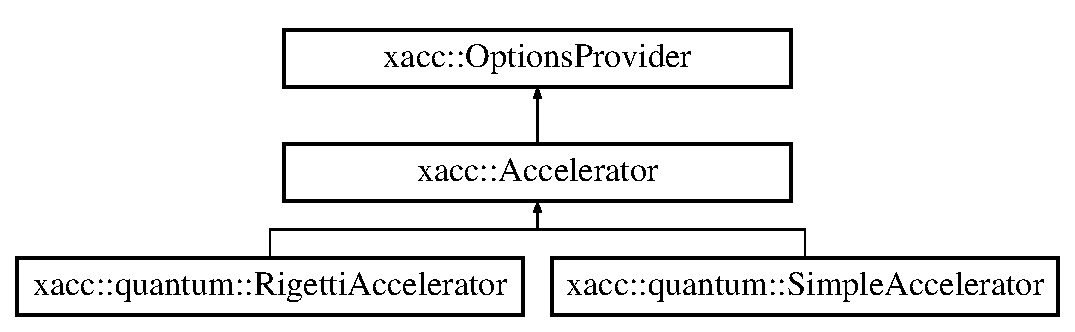
\includegraphics[height=2.679426cm]{a00011}
\end{center}
\end{figure}
\subsection*{Public Member Functions}
\begin{DoxyCompactItemize}
\item 
virtual void \hyperlink{a00011_a8cdc6f0c5a660013c29c07657a06303b}{initialize} ()=0
\item 
virtual Accelerator\+Type \hyperlink{a00011_aaffc3e4bb9880eb5041b1b58ee4c2665}{get\+Type} ()=0
\item 
virtual std\+::vector$<$ \hyperlink{a00051}{I\+R\+Transformation} $>$ \hyperlink{a00011_ad6e4a642dcb24e552675bcbeff1e1b04}{get\+I\+R\+Transformations} ()=0
\item 
virtual void \hyperlink{a00011_a89b3f3e6294f228abf03a410b0fb1674}{execute} (std\+::shared\+\_\+ptr$<$ \hyperlink{a00013}{Accelerator\+Buffer} $>$ buffer, const std\+::shared\+\_\+ptr$<$ \hyperlink{a00038}{Function} $>$ function)=0
\item 
virtual std\+::shared\+\_\+ptr$<$ \hyperlink{a00013}{Accelerator\+Buffer} $>$ \hyperlink{a00011_aab5046e8d83ab390302e0f49533e95fc}{create\+Buffer} (const std\+::string \&var\+Id)=0
\item 
virtual std\+::shared\+\_\+ptr$<$ \hyperlink{a00013}{Accelerator\+Buffer} $>$ \hyperlink{a00011_a064a2dbd58338364115c260267806945}{create\+Buffer} (const std\+::string \&var\+Id, const int size)=0
\item 
virtual std\+::shared\+\_\+ptr$<$ \hyperlink{a00013}{Accelerator\+Buffer} $>$ \hyperlink{a00011_ab3820be326e28a553fed1a824f4d41d0}{get\+Buffer} (const std\+::string \&varid)
\item 
virtual std\+::vector$<$ std\+::string $>$ \hyperlink{a00011_ae1463d7e405df89fa4af47e8922f4b82}{get\+Allocated\+Buffer\+Names} ()
\item 
virtual std\+::shared\+\_\+ptr$<$ \hyperlink{a00043}{Accelerator\+Graph} $>$ \hyperlink{a00011_adfed940ce1fa476b009344ddf5a4bbc3}{get\+Accelerator\+Connectivity} ()
\item 
virtual std\+::shared\+\_\+ptr$<$ options\+\_\+description $>$ \hyperlink{a00011_a98c9eda6b54367c75667ecfbbf167979}{get\+Options} ()
\item 
virtual \hyperlink{a00011_aed88ab0d71b765f0b0f512684ccd4b55}{$\sim$\+Accelerator} ()
\end{DoxyCompactItemize}
\subsection*{Protected Member Functions}
\begin{DoxyCompactItemize}
\item 
virtual bool \hyperlink{a00011_ae51584850faeec77299058383977ddeb}{is\+Valid\+Buffer\+Size} (const int N\+Bits)=0
\item 
void \hyperlink{a00011_ac3e781f42ec25e460174d4c41ea26b94}{store\+Buffer} (const std\+::string \&id, std\+::shared\+\_\+ptr$<$ \hyperlink{a00013}{Accelerator\+Buffer} $>$ b)
\end{DoxyCompactItemize}


\subsection{Detailed Description}
The \hyperlink{a00011}{Accelerator} class provides a high-\/level abstraction for X\+A\+CC\textquotesingle{}s interaction with attached post-\/exascale accelerators (quantum and neuromorphic processing units).

Derived Accelerators must provide a valid execute implementation that takes X\+A\+CC \hyperlink{a00050}{IR} and executes it on the attached hardware or simulator.

Derived Accelerators must provide a list of \hyperlink{a00051}{I\+R\+Transformation} instances that transform X\+A\+CC \hyperlink{a00050}{IR} to be amenable to execution on the hardware.

Derived Accelerators must provide implementations of create\+Buffer that provide a valid \hyperlink{a00013}{Accelerator\+Buffer} instance modeling the hardware memory or bits being computed on. Upon creating an \hyperlink{a00013}{Accelerator\+Buffer}, derived \hyperlink{a00011}{Accelerator} implementations must call the protected store\+Buffer method to store the \hyperlink{a00013}{Accelerator\+Buffer} for future reference by Compilers and clients of \hyperlink{a00011}{Accelerator}.

\begin{DoxyAuthor}{Author}
Alex Mc\+Caskey 
\end{DoxyAuthor}


\subsection{Constructor \& Destructor Documentation}
\index{xacc\+::\+Accelerator@{xacc\+::\+Accelerator}!````~Accelerator@{$\sim$\+Accelerator}}
\index{````~Accelerator@{$\sim$\+Accelerator}!xacc\+::\+Accelerator@{xacc\+::\+Accelerator}}
\subsubsection[{\texorpdfstring{$\sim$\+Accelerator()}{~Accelerator()}}]{\setlength{\rightskip}{0pt plus 5cm}virtual xacc\+::\+Accelerator\+::$\sim$\+Accelerator (
\begin{DoxyParamCaption}
{}
\end{DoxyParamCaption}
)\hspace{0.3cm}{\ttfamily [inline]}, {\ttfamily [virtual]}}\hypertarget{a00011_aed88ab0d71b765f0b0f512684ccd4b55}{}\label{a00011_aed88ab0d71b765f0b0f512684ccd4b55}
Destructor 

\subsection{Member Function Documentation}
\index{xacc\+::\+Accelerator@{xacc\+::\+Accelerator}!create\+Buffer@{create\+Buffer}}
\index{create\+Buffer@{create\+Buffer}!xacc\+::\+Accelerator@{xacc\+::\+Accelerator}}
\subsubsection[{\texorpdfstring{create\+Buffer(const std\+::string \&var\+Id)=0}{createBuffer(const std::string \&varId)=0}}]{\setlength{\rightskip}{0pt plus 5cm}virtual std\+::shared\+\_\+ptr$<${\bf Accelerator\+Buffer}$>$ xacc\+::\+Accelerator\+::create\+Buffer (
\begin{DoxyParamCaption}
\item[{const std\+::string \&}]{var\+Id}
\end{DoxyParamCaption}
)\hspace{0.3cm}{\ttfamily [pure virtual]}}\hypertarget{a00011_aab5046e8d83ab390302e0f49533e95fc}{}\label{a00011_aab5046e8d83ab390302e0f49533e95fc}
Create, store, and return an \hyperlink{a00013}{Accelerator\+Buffer} with the given variable id string. This method returns all available qubits for this \hyperlink{a00011}{Accelerator}. The string id serves as a unique identifier for future lookups and reuse of the \hyperlink{a00013}{Accelerator\+Buffer}.


\begin{DoxyParams}{Parameters}
{\em var\+Id} & The variable name of the created buffer \\
\hline
\end{DoxyParams}
\begin{DoxyReturn}{Returns}
buffer The buffer instance created. 
\end{DoxyReturn}


Implemented in \hyperlink{a00029_add60637a4b3c055e7f2ffa3bf8e320ac}{xacc\+::quantum\+::\+D\+W\+Accelerator}, \hyperlink{a00079_a46445d77d4b8ad2689571d0db6604380}{xacc\+::quantum\+::\+Simple\+Accelerator}, and \hyperlink{a00071_ada3ceb986e51ab5aa721f2a08e083cd6}{xacc\+::quantum\+::\+Rigetti\+Accelerator}.

\index{xacc\+::\+Accelerator@{xacc\+::\+Accelerator}!create\+Buffer@{create\+Buffer}}
\index{create\+Buffer@{create\+Buffer}!xacc\+::\+Accelerator@{xacc\+::\+Accelerator}}
\subsubsection[{\texorpdfstring{create\+Buffer(const std\+::string \&var\+Id, const int size)=0}{createBuffer(const std::string \&varId, const int size)=0}}]{\setlength{\rightskip}{0pt plus 5cm}virtual std\+::shared\+\_\+ptr$<${\bf Accelerator\+Buffer}$>$ xacc\+::\+Accelerator\+::create\+Buffer (
\begin{DoxyParamCaption}
\item[{const std\+::string \&}]{var\+Id, }
\item[{const int}]{size}
\end{DoxyParamCaption}
)\hspace{0.3cm}{\ttfamily [pure virtual]}}\hypertarget{a00011_a064a2dbd58338364115c260267806945}{}\label{a00011_a064a2dbd58338364115c260267806945}
Create, store, and return an \hyperlink{a00013}{Accelerator\+Buffer} with the given variable id string and of the given number of bits. The string id serves as a unique identifier for future lookups and reuse of the \hyperlink{a00013}{Accelerator\+Buffer}.


\begin{DoxyParams}{Parameters}
{\em var\+Id} & The variable name of the created buffer \\
\hline
{\em size} & The number of bits in the created buffer \\
\hline
\end{DoxyParams}
\begin{DoxyReturn}{Returns}
buffer The buffer instance created. 
\end{DoxyReturn}


Implemented in \hyperlink{a00029_a718d7cb51a35e694d960385e1ea2f99f}{xacc\+::quantum\+::\+D\+W\+Accelerator}, \hyperlink{a00071_a731551c94b1abef40d2cf032e8712df6}{xacc\+::quantum\+::\+Rigetti\+Accelerator}, and \hyperlink{a00079_adb9393692e9f484df241aa5d014030d1}{xacc\+::quantum\+::\+Simple\+Accelerator}.

\index{xacc\+::\+Accelerator@{xacc\+::\+Accelerator}!execute@{execute}}
\index{execute@{execute}!xacc\+::\+Accelerator@{xacc\+::\+Accelerator}}
\subsubsection[{\texorpdfstring{execute(std\+::shared\+\_\+ptr$<$ Accelerator\+Buffer $>$ buffer, const std\+::shared\+\_\+ptr$<$ Function $>$ function)=0}{execute(std::shared\_ptr< AcceleratorBuffer > buffer, const std::shared\_ptr< Function > function)=0}}]{\setlength{\rightskip}{0pt plus 5cm}virtual void xacc\+::\+Accelerator\+::execute (
\begin{DoxyParamCaption}
\item[{std\+::shared\+\_\+ptr$<$ {\bf Accelerator\+Buffer} $>$}]{buffer, }
\item[{const std\+::shared\+\_\+ptr$<$ {\bf Function} $>$}]{function}
\end{DoxyParamCaption}
)\hspace{0.3cm}{\ttfamily [pure virtual]}}\hypertarget{a00011_a89b3f3e6294f228abf03a410b0fb1674}{}\label{a00011_a89b3f3e6294f228abf03a410b0fb1674}
Execute the provided X\+A\+CC \hyperlink{a00050}{IR} \hyperlink{a00038}{Function} on the provided \hyperlink{a00013}{Accelerator\+Buffer}.


\begin{DoxyParams}{Parameters}
{\em buffer} & The buffer of bits this \hyperlink{a00011}{Accelerator} should operate on. \\
\hline
{\em function} & The kernel to execute. \\
\hline
\end{DoxyParams}
\index{xacc\+::\+Accelerator@{xacc\+::\+Accelerator}!get\+Accelerator\+Connectivity@{get\+Accelerator\+Connectivity}}
\index{get\+Accelerator\+Connectivity@{get\+Accelerator\+Connectivity}!xacc\+::\+Accelerator@{xacc\+::\+Accelerator}}
\subsubsection[{\texorpdfstring{get\+Accelerator\+Connectivity()}{getAcceleratorConnectivity()}}]{\setlength{\rightskip}{0pt plus 5cm}virtual std\+::shared\+\_\+ptr$<${\bf Accelerator\+Graph}$>$ xacc\+::\+Accelerator\+::get\+Accelerator\+Connectivity (
\begin{DoxyParamCaption}
{}
\end{DoxyParamCaption}
)\hspace{0.3cm}{\ttfamily [inline]}, {\ttfamily [virtual]}}\hypertarget{a00011_adfed940ce1fa476b009344ddf5a4bbc3}{}\label{a00011_adfed940ce1fa476b009344ddf5a4bbc3}
Return the graph structure for this \hyperlink{a00011}{Accelerator}.

\begin{DoxyReturn}{Returns}
connectivity\+Graph The graph structure of this \hyperlink{a00011}{Accelerator} 
\end{DoxyReturn}


Reimplemented in \hyperlink{a00029_a006afa60749790681fc76beddc254926}{xacc\+::quantum\+::\+D\+W\+Accelerator}.

\index{xacc\+::\+Accelerator@{xacc\+::\+Accelerator}!get\+Allocated\+Buffer\+Names@{get\+Allocated\+Buffer\+Names}}
\index{get\+Allocated\+Buffer\+Names@{get\+Allocated\+Buffer\+Names}!xacc\+::\+Accelerator@{xacc\+::\+Accelerator}}
\subsubsection[{\texorpdfstring{get\+Allocated\+Buffer\+Names()}{getAllocatedBufferNames()}}]{\setlength{\rightskip}{0pt plus 5cm}virtual std\+::vector$<$std\+::string$>$ xacc\+::\+Accelerator\+::get\+Allocated\+Buffer\+Names (
\begin{DoxyParamCaption}
{}
\end{DoxyParamCaption}
)\hspace{0.3cm}{\ttfamily [inline]}, {\ttfamily [virtual]}}\hypertarget{a00011_ae1463d7e405df89fa4af47e8922f4b82}{}\label{a00011_ae1463d7e405df89fa4af47e8922f4b82}
Return all allocated \hyperlink{a00013}{Accelerator\+Buffer} variable names.

\begin{DoxyReturn}{Returns}
var\+Names The buffer variable names 
\end{DoxyReturn}
\index{xacc\+::\+Accelerator@{xacc\+::\+Accelerator}!get\+Buffer@{get\+Buffer}}
\index{get\+Buffer@{get\+Buffer}!xacc\+::\+Accelerator@{xacc\+::\+Accelerator}}
\subsubsection[{\texorpdfstring{get\+Buffer(const std\+::string \&varid)}{getBuffer(const std::string \&varid)}}]{\setlength{\rightskip}{0pt plus 5cm}virtual std\+::shared\+\_\+ptr$<${\bf Accelerator\+Buffer}$>$ xacc\+::\+Accelerator\+::get\+Buffer (
\begin{DoxyParamCaption}
\item[{const std\+::string \&}]{varid}
\end{DoxyParamCaption}
)\hspace{0.3cm}{\ttfamily [inline]}, {\ttfamily [virtual]}}\hypertarget{a00011_ab3820be326e28a553fed1a824f4d41d0}{}\label{a00011_ab3820be326e28a553fed1a824f4d41d0}
Return the stored \hyperlink{a00013}{Accelerator\+Buffer} with the provided string id.


\begin{DoxyParams}{Parameters}
{\em varid} & The variable name of the created buffer \\
\hline
\end{DoxyParams}
\begin{DoxyReturn}{Returns}
buffer The buffer with given varid. 
\end{DoxyReturn}
\index{xacc\+::\+Accelerator@{xacc\+::\+Accelerator}!get\+I\+R\+Transformations@{get\+I\+R\+Transformations}}
\index{get\+I\+R\+Transformations@{get\+I\+R\+Transformations}!xacc\+::\+Accelerator@{xacc\+::\+Accelerator}}
\subsubsection[{\texorpdfstring{get\+I\+R\+Transformations()=0}{getIRTransformations()=0}}]{\setlength{\rightskip}{0pt plus 5cm}virtual std\+::vector$<${\bf I\+R\+Transformation}$>$ xacc\+::\+Accelerator\+::get\+I\+R\+Transformations (
\begin{DoxyParamCaption}
{}
\end{DoxyParamCaption}
)\hspace{0.3cm}{\ttfamily [pure virtual]}}\hypertarget{a00011_ad6e4a642dcb24e552675bcbeff1e1b04}{}\label{a00011_ad6e4a642dcb24e552675bcbeff1e1b04}
Return any \hyperlink{a00050}{IR} Transformations that must be applied to ensure the compiled \hyperlink{a00050}{IR} is amenable to execution on this \hyperlink{a00011}{Accelerator}.

\begin{DoxyReturn}{Returns}
transformations The \hyperlink{a00050}{IR} transformations this \hyperlink{a00011}{Accelerator} exposes 
\end{DoxyReturn}


Implemented in \hyperlink{a00029_a89da20bd079a22d6581ea2da2293b973}{xacc\+::quantum\+::\+D\+W\+Accelerator}, \hyperlink{a00071_a443683a1dfb000603c640b2ee303cf66}{xacc\+::quantum\+::\+Rigetti\+Accelerator}, and \hyperlink{a00079_afc49c9e7973ba6c6ff9761c36198323d}{xacc\+::quantum\+::\+Simple\+Accelerator}.

\index{xacc\+::\+Accelerator@{xacc\+::\+Accelerator}!get\+Options@{get\+Options}}
\index{get\+Options@{get\+Options}!xacc\+::\+Accelerator@{xacc\+::\+Accelerator}}
\subsubsection[{\texorpdfstring{get\+Options()}{getOptions()}}]{\setlength{\rightskip}{0pt plus 5cm}virtual std\+::shared\+\_\+ptr$<$options\+\_\+description$>$ xacc\+::\+Accelerator\+::get\+Options (
\begin{DoxyParamCaption}
{}
\end{DoxyParamCaption}
)\hspace{0.3cm}{\ttfamily [inline]}, {\ttfamily [virtual]}}\hypertarget{a00011_a98c9eda6b54367c75667ecfbbf167979}{}\label{a00011_a98c9eda6b54367c75667ecfbbf167979}
Return an empty options\+\_\+description, this is for subclasses to implement. 

Implements \hyperlink{a00056_a6d150954f852109bfe2c1ae90222926f}{xacc\+::\+Options\+Provider}.



Reimplemented in \hyperlink{a00029_a09926db9f99706307ae6ce5b56845bca}{xacc\+::quantum\+::\+D\+W\+Accelerator}, and \hyperlink{a00071_a9ee9e62aecbccf193894ca3388676f9f}{xacc\+::quantum\+::\+Rigetti\+Accelerator}.

\index{xacc\+::\+Accelerator@{xacc\+::\+Accelerator}!get\+Type@{get\+Type}}
\index{get\+Type@{get\+Type}!xacc\+::\+Accelerator@{xacc\+::\+Accelerator}}
\subsubsection[{\texorpdfstring{get\+Type()=0}{getType()=0}}]{\setlength{\rightskip}{0pt plus 5cm}virtual Accelerator\+Type xacc\+::\+Accelerator\+::get\+Type (
\begin{DoxyParamCaption}
{}
\end{DoxyParamCaption}
)\hspace{0.3cm}{\ttfamily [pure virtual]}}\hypertarget{a00011_aaffc3e4bb9880eb5041b1b58ee4c2665}{}\label{a00011_aaffc3e4bb9880eb5041b1b58ee4c2665}
Return the type of this \hyperlink{a00011}{Accelerator}.

\begin{DoxyReturn}{Returns}
type The \hyperlink{a00011}{Accelerator} type -\/ Gate or A\+QC Q\+PU, or N\+PU 
\end{DoxyReturn}


Implemented in \hyperlink{a00029_abe50e427b4bec0460cc238405cb569f9}{xacc\+::quantum\+::\+D\+W\+Accelerator}, \hyperlink{a00071_aab0d4674da5273d55407b9ab77cde890}{xacc\+::quantum\+::\+Rigetti\+Accelerator}, and \hyperlink{a00079_ad76eeb0bbd7de21aad5bd20d20970a98}{xacc\+::quantum\+::\+Simple\+Accelerator}.

\index{xacc\+::\+Accelerator@{xacc\+::\+Accelerator}!initialize@{initialize}}
\index{initialize@{initialize}!xacc\+::\+Accelerator@{xacc\+::\+Accelerator}}
\subsubsection[{\texorpdfstring{initialize()=0}{initialize()=0}}]{\setlength{\rightskip}{0pt plus 5cm}virtual void xacc\+::\+Accelerator\+::initialize (
\begin{DoxyParamCaption}
{}
\end{DoxyParamCaption}
)\hspace{0.3cm}{\ttfamily [pure virtual]}}\hypertarget{a00011_a8cdc6f0c5a660013c29c07657a06303b}{}\label{a00011_a8cdc6f0c5a660013c29c07657a06303b}
Initialize this \hyperlink{a00011}{Accelerator}. This method is called by the X\+A\+CC framework after an \hyperlink{a00011}{Accelerator} has been requested and created. Perform any work you need done before execution here. 

Implemented in \hyperlink{a00029_acaefd5747409f31cf5c3e42d98475ce2}{xacc\+::quantum\+::\+D\+W\+Accelerator}, \hyperlink{a00071_ab8b6af9bb9dcb110201e9ee5cac74b4f}{xacc\+::quantum\+::\+Rigetti\+Accelerator}, and \hyperlink{a00079_a392e3b30523f5f681127e7e98887108c}{xacc\+::quantum\+::\+Simple\+Accelerator}.

\index{xacc\+::\+Accelerator@{xacc\+::\+Accelerator}!is\+Valid\+Buffer\+Size@{is\+Valid\+Buffer\+Size}}
\index{is\+Valid\+Buffer\+Size@{is\+Valid\+Buffer\+Size}!xacc\+::\+Accelerator@{xacc\+::\+Accelerator}}
\subsubsection[{\texorpdfstring{is\+Valid\+Buffer\+Size(const int N\+Bits)=0}{isValidBufferSize(const int NBits)=0}}]{\setlength{\rightskip}{0pt plus 5cm}virtual bool xacc\+::\+Accelerator\+::is\+Valid\+Buffer\+Size (
\begin{DoxyParamCaption}
\item[{const int}]{N\+Bits}
\end{DoxyParamCaption}
)\hspace{0.3cm}{\ttfamily [protected]}, {\ttfamily [pure virtual]}}\hypertarget{a00011_ae51584850faeec77299058383977ddeb}{}\label{a00011_ae51584850faeec77299058383977ddeb}
Return true if this \hyperlink{a00011}{Accelerator} can allocated N\+Bits number of bits. This is meant to be implemented and used by subclasses.


\begin{DoxyParams}{Parameters}
{\em N\+Bits} & The number of bits to allocate \\
\hline
\end{DoxyParams}
\begin{DoxyReturn}{Returns}
valid True if size is valid. 
\end{DoxyReturn}


Implemented in \hyperlink{a00029_a4c2ee30212a919d8ddf7f9555df25195}{xacc\+::quantum\+::\+D\+W\+Accelerator}, \hyperlink{a00079_a60b9db2d6aed235857c45413a070338e}{xacc\+::quantum\+::\+Simple\+Accelerator}, and \hyperlink{a00071_a61352c07062597aad2393fbeed4cc025}{xacc\+::quantum\+::\+Rigetti\+Accelerator}.

\index{xacc\+::\+Accelerator@{xacc\+::\+Accelerator}!store\+Buffer@{store\+Buffer}}
\index{store\+Buffer@{store\+Buffer}!xacc\+::\+Accelerator@{xacc\+::\+Accelerator}}
\subsubsection[{\texorpdfstring{store\+Buffer(const std\+::string \&id, std\+::shared\+\_\+ptr$<$ Accelerator\+Buffer $>$ b)}{storeBuffer(const std::string \&id, std::shared\_ptr< AcceleratorBuffer > b)}}]{\setlength{\rightskip}{0pt plus 5cm}void xacc\+::\+Accelerator\+::store\+Buffer (
\begin{DoxyParamCaption}
\item[{const std\+::string \&}]{id, }
\item[{std\+::shared\+\_\+ptr$<$ {\bf Accelerator\+Buffer} $>$}]{b}
\end{DoxyParamCaption}
)\hspace{0.3cm}{\ttfamily [inline]}, {\ttfamily [protected]}}\hypertarget{a00011_ac3e781f42ec25e460174d4c41ea26b94}{}\label{a00011_ac3e781f42ec25e460174d4c41ea26b94}
This protected method is to be used by derived Accelerators to store any created \hyperlink{a00013}{Accelerator\+Buffer}.


\begin{DoxyParams}{Parameters}
{\em id} & The variable name of the buffer to store \\
\hline
{\em b} & The buffer to store \\
\hline
\end{DoxyParams}


The documentation for this class was generated from the following file\+:\begin{DoxyCompactItemize}
\item 
Accelerator.\+hpp\end{DoxyCompactItemize}

\hypertarget{a00012}{}\section{xacc\+:\+:Accelerator\+Bit Class Reference}
\label{a00012}\index{xacc\+::\+Accelerator\+Bit@{xacc\+::\+Accelerator\+Bit}}


{\ttfamily \#include $<$Accelerator\+Buffer.\+hpp$>$}

\subsection*{Public Member Functions}
\begin{DoxyCompactItemize}
\item 
\hyperlink{a00012_a9a124c230c5cabeab53bac0820c0221a}{Accelerator\+Bit} ()
\item 
void \hyperlink{a00012_aa63a24980e831b9325a36836ab1c5495}{update} (int zero\+Or\+One)
\item 
Accelerator\+Bit\+State \hyperlink{a00012_a4a8dcc4fa02a5619f583961460c77057}{get\+State} ()
\end{DoxyCompactItemize}
\subsection*{Protected Attributes}
\begin{DoxyCompactItemize}
\item 
Accelerator\+Bit\+State \hyperlink{a00012_a4632123ac31aeed0dc97c65f8c792a85}{state}
\end{DoxyCompactItemize}


\subsection{Detailed Description}
The \hyperlink{a00012}{Accelerator\+Bit} wraps an Accelerator\+Bit\+Sate and provides a mechanism for updating that state.

\begin{DoxyAuthor}{Author}
Alex Mc\+Caskey 
\end{DoxyAuthor}


\subsection{Constructor \& Destructor Documentation}
\index{xacc\+::\+Accelerator\+Bit@{xacc\+::\+Accelerator\+Bit}!Accelerator\+Bit@{Accelerator\+Bit}}
\index{Accelerator\+Bit@{Accelerator\+Bit}!xacc\+::\+Accelerator\+Bit@{xacc\+::\+Accelerator\+Bit}}
\subsubsection[{\texorpdfstring{Accelerator\+Bit()}{AcceleratorBit()}}]{\setlength{\rightskip}{0pt plus 5cm}xacc\+::\+Accelerator\+Bit\+::\+Accelerator\+Bit (
\begin{DoxyParamCaption}
{}
\end{DoxyParamCaption}
)\hspace{0.3cm}{\ttfamily [inline]}}\hypertarget{a00012_a9a124c230c5cabeab53bac0820c0221a}{}\label{a00012_a9a124c230c5cabeab53bac0820c0221a}
The constructor, all bits are initialized to unknown state 

\subsection{Member Function Documentation}
\index{xacc\+::\+Accelerator\+Bit@{xacc\+::\+Accelerator\+Bit}!get\+State@{get\+State}}
\index{get\+State@{get\+State}!xacc\+::\+Accelerator\+Bit@{xacc\+::\+Accelerator\+Bit}}
\subsubsection[{\texorpdfstring{get\+State()}{getState()}}]{\setlength{\rightskip}{0pt plus 5cm}Accelerator\+Bit\+State xacc\+::\+Accelerator\+Bit\+::get\+State (
\begin{DoxyParamCaption}
{}
\end{DoxyParamCaption}
)\hspace{0.3cm}{\ttfamily [inline]}}\hypertarget{a00012_a4a8dcc4fa02a5619f583961460c77057}{}\label{a00012_a4a8dcc4fa02a5619f583961460c77057}
Return the value of this state \index{xacc\+::\+Accelerator\+Bit@{xacc\+::\+Accelerator\+Bit}!update@{update}}
\index{update@{update}!xacc\+::\+Accelerator\+Bit@{xacc\+::\+Accelerator\+Bit}}
\subsubsection[{\texorpdfstring{update(int zero\+Or\+One)}{update(int zeroOrOne)}}]{\setlength{\rightskip}{0pt plus 5cm}void xacc\+::\+Accelerator\+Bit\+::update (
\begin{DoxyParamCaption}
\item[{int}]{zero\+Or\+One}
\end{DoxyParamCaption}
)\hspace{0.3cm}{\ttfamily [inline]}}\hypertarget{a00012_aa63a24980e831b9325a36836ab1c5495}{}\label{a00012_aa63a24980e831b9325a36836ab1c5495}
Update the Bit state to a one or zero 

\subsection{Member Data Documentation}
\index{xacc\+::\+Accelerator\+Bit@{xacc\+::\+Accelerator\+Bit}!state@{state}}
\index{state@{state}!xacc\+::\+Accelerator\+Bit@{xacc\+::\+Accelerator\+Bit}}
\subsubsection[{\texorpdfstring{state}{state}}]{\setlength{\rightskip}{0pt plus 5cm}Accelerator\+Bit\+State xacc\+::\+Accelerator\+Bit\+::state\hspace{0.3cm}{\ttfamily [protected]}}\hypertarget{a00012_a4632123ac31aeed0dc97c65f8c792a85}{}\label{a00012_a4632123ac31aeed0dc97c65f8c792a85}
The bit state 

The documentation for this class was generated from the following file\+:\begin{DoxyCompactItemize}
\item 
Accelerator\+Buffer.\+hpp\end{DoxyCompactItemize}

\hypertarget{a00013}{}\section{xacc\+:\+:Accelerator\+Buffer Class Reference}
\label{a00013}\index{xacc\+::\+Accelerator\+Buffer@{xacc\+::\+Accelerator\+Buffer}}


{\ttfamily \#include $<$Accelerator\+Buffer.\+hpp$>$}

Inheritance diagram for xacc\+:\+:Accelerator\+Buffer\+:\begin{figure}[H]
\begin{center}
\leavevmode
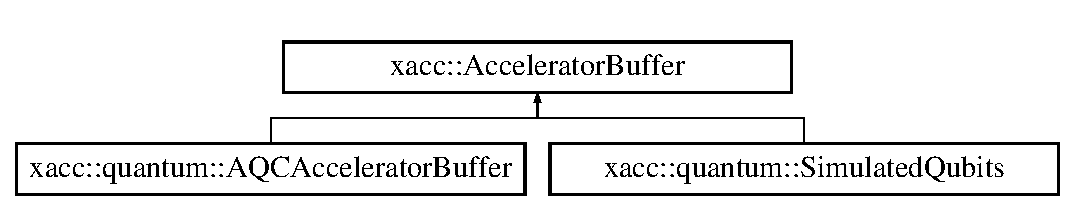
\includegraphics[height=2.000000cm]{a00013}
\end{center}
\end{figure}
\subsection*{Public Member Functions}
\begin{DoxyCompactItemize}
\item 
\hyperlink{a00013_ab606d8af942120d60b51a4fffcd75c98}{Accelerator\+Buffer} (const std\+::string \&str, const int N)
\item 
{\footnotesize template$<$typename... Indices$>$ }\\{\bfseries Accelerator\+Buffer} (const std\+::string \&str, int first\+Index, Indices...\+indices)\hypertarget{a00013_ac550d89390562095c56aa1b14ae85001}{}\label{a00013_ac550d89390562095c56aa1b14ae85001}

\item 
int {\bfseries size} ()\hypertarget{a00013_aa2a3101c2e3ae3550172bf49f9587f3b}{}\label{a00013_aa2a3101c2e3ae3550172bf49f9587f3b}

\item 
std\+::string {\bfseries name} ()\hypertarget{a00013_ad5b646e9efc21b6d0bcc22cd6f649c22}{}\label{a00013_ad5b646e9efc21b6d0bcc22cd6f649c22}

\item 
void {\bfseries reset\+Buffer} ()\hypertarget{a00013_aa6d6e9cfee6170333c1f03507345743f}{}\label{a00013_aa6d6e9cfee6170333c1f03507345743f}

\item 
void {\bfseries update\+Bit} (const int idx, int zero\+Or\+One)\hypertarget{a00013_a4bc0edbe9aa0d463f67ddcc38265066f}{}\label{a00013_a4bc0edbe9aa0d463f67ddcc38265066f}

\item 
void {\bfseries append\+Measurement} (const boost\+::dynamic\+\_\+bitset$<$$>$ \&measurement)\hypertarget{a00013_ac161c4f984f774d08197871094aabc67}{}\label{a00013_ac161c4f984f774d08197871094aabc67}

\item 
double {\bfseries get\+Average} () const \hypertarget{a00013_a97cf3cc4e1aaa8ac3cee7817860f77c1}{}\label{a00013_a97cf3cc4e1aaa8ac3cee7817860f77c1}

\item 
Accelerator\+Bit\+State {\bfseries get\+Accelerator\+Bit\+State} (const int idx)\hypertarget{a00013_aba6ef359f3117faa98f0eb8da90d909e}{}\label{a00013_aba6ef359f3117faa98f0eb8da90d909e}

\item 
virtual void {\bfseries print} ()\hypertarget{a00013_add0835e188f0eda4f1b68a28ddc79786}{}\label{a00013_add0835e188f0eda4f1b68a28ddc79786}

\item 
virtual void {\bfseries print} (std\+::ostream \&stream)\hypertarget{a00013_a7c59462451223772b41ef232b06a7dfa}{}\label{a00013_a7c59462451223772b41ef232b06a7dfa}

\end{DoxyCompactItemize}
\subsection*{Protected Attributes}
\begin{DoxyCompactItemize}
\item 
std\+::vector$<$ boost\+::dynamic\+\_\+bitset$<$$>$ $>$ {\bfseries measurements}\hypertarget{a00013_a5464b23a964985df2547f657877c9ea5}{}\label{a00013_a5464b23a964985df2547f657877c9ea5}

\item 
std\+::string {\bfseries buffer\+Id}\hypertarget{a00013_a3198e034d07d9b77b62da03e6592a221}{}\label{a00013_a3198e034d07d9b77b62da03e6592a221}

\item 
std\+::vector$<$ \hyperlink{a00012}{Accelerator\+Bit} $>$ {\bfseries bits}\hypertarget{a00013_ab6dbb8c22f8adc6aba34b00a84066854}{}\label{a00013_ab6dbb8c22f8adc6aba34b00a84066854}

\end{DoxyCompactItemize}


\subsection{Detailed Description}
The \hyperlink{a00013}{Accelerator\+Buffer} models an allocated buffer of bits that are operated on by a kernel. As such, the \hyperlink{a00013}{Accelerator\+Buffer}\textquotesingle{}s primary role is to store \hyperlink{a00011}{Accelerator} execution results.

\begin{DoxyAuthor}{Author}
Alex Mc\+Caskey 
\end{DoxyAuthor}


\subsection{Constructor \& Destructor Documentation}
\index{xacc\+::\+Accelerator\+Buffer@{xacc\+::\+Accelerator\+Buffer}!Accelerator\+Buffer@{Accelerator\+Buffer}}
\index{Accelerator\+Buffer@{Accelerator\+Buffer}!xacc\+::\+Accelerator\+Buffer@{xacc\+::\+Accelerator\+Buffer}}
\subsubsection[{\texorpdfstring{Accelerator\+Buffer(const std\+::string \&str, const int N)}{AcceleratorBuffer(const std::string \&str, const int N)}}]{\setlength{\rightskip}{0pt plus 5cm}xacc\+::\+Accelerator\+Buffer\+::\+Accelerator\+Buffer (
\begin{DoxyParamCaption}
\item[{const std\+::string \&}]{str, }
\item[{const int}]{N}
\end{DoxyParamCaption}
)\hspace{0.3cm}{\ttfamily [inline]}}\hypertarget{a00013_ab606d8af942120d60b51a4fffcd75c98}{}\label{a00013_ab606d8af942120d60b51a4fffcd75c98}
The Constructor 

The documentation for this class was generated from the following file\+:\begin{DoxyCompactItemize}
\item 
Accelerator\+Buffer.\+hpp\end{DoxyCompactItemize}

\hypertarget{a00014}{}\section{xacc\+:\+:quantum\+:\+:All\+Gate\+Visitor Class Reference}
\label{a00014}\index{xacc\+::quantum\+::\+All\+Gate\+Visitor@{xacc\+::quantum\+::\+All\+Gate\+Visitor}}


{\ttfamily \#include $<$All\+Gate\+Visitor.\+hpp$>$}

Inheritance diagram for xacc\+:\+:quantum\+:\+:All\+Gate\+Visitor\+:\begin{figure}[H]
\begin{center}
\leavevmode
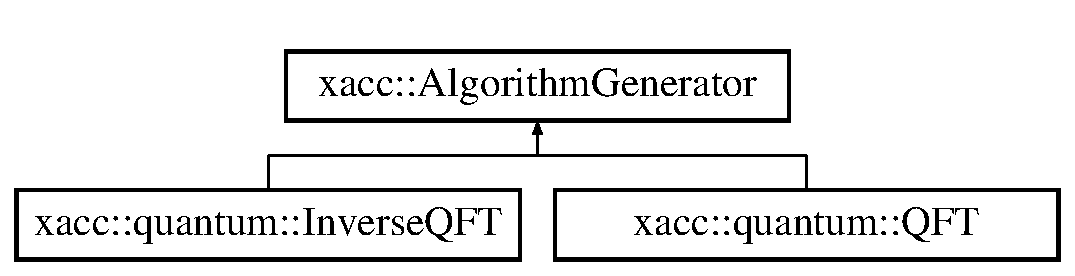
\includegraphics[height=9.201878cm]{a00014}
\end{center}
\end{figure}
\subsection*{Additional Inherited Members}


\subsection{Detailed Description}
F\+I\+X\+ME write this 

The documentation for this class was generated from the following file\+:\begin{DoxyCompactItemize}
\item 
All\+Gate\+Visitor.\+hpp\end{DoxyCompactItemize}



 layout\+: post title\+: Astrophysics Reactions \hyperlink{a00038}{A\+S\+C\+II} File Format permalink\+: /science/astrophysics/reactions-\/ascii-\/format \subsection*{category\+: science }

Simulations of thermonuclear networks in astrophysics require lists of reactions that describe how the species evolve over time. Fire supports a legacy \hyperlink{a00038}{A\+S\+C\+II} format with a 8-\/line specification for a reaction. Each entry in each line is separated by a space. See \hyperlink{a00678_source}{Reaction.\+h} for full details on each required value.

The first line for each reaction contains\+:


\begin{DoxyItemize}
\item Name/\+Label -\/ A string of the form \char`\"{}he4+he4+he4-\/-\/$>$c12\char`\"{} that describes the reaction.
\item Reaction Group Class -\/ an integer
\item Reaction Group Index -\/ an integer
\item R\+E\+A\+C\+L\+IB Class -\/ an integer
\item Number of reacting species -\/ an integer
\item Number of resulting products -\/ an integer
\item Electron capture flag -\/ a bool
\item Reverse reaction flag -\/ a bool
\item Statistical factor -\/ a double
\item Energy release -\/ a double
\end{DoxyItemize}

The second line contains the seven rate coefficients from the R\+E\+A\+C\+L\+IB library, all doubles. The third line contains the array of atomic numbers for the reactants in this reaction, which are integers. The fourth, fifth, and sixth lines are also integers for the reactant neutron number and product atomic and neutron numbers. Each of these four lines has one integer for each reactant and product in the system, but with no more than four entries per line. (See example below for more details.)

The seventh and eighth lines contain quantities that are used for {\itshape Partial Equilibrium} approximations. Each line contains up to three integers.


\begin{DoxyCode}
1 he4+he4+he4-->c12 3 0 8 3 1 0 0 0.16666667 7.27500
2 -24.99350000 -4.29702000 -6.69304000 15.59030000 -1.57387000 0.17058800 -9.02800000
3 2 2 2 // Since numReactants = 3 and he4 has Z=2, there are three values on this line equal to 2.
4 2 2 2 // Same, but for he4's neutron number
5 6 // There is only one product and Z=6 for C12.
6 6 // N=6 for C12
7 0 0 0 
8 1 
9 ne20-->he4+o16 2 3 2 1 2 0 1 1.00000000 -4.73400
10 109.31000000 -72.75840000 293.66400000 -384.97400000 20.23800000 -1.00379000 201.19300000
11 10 // Z for ne20
12 10 // N for ne20
13 2 8 // Z for he4 and o16
14 2 8 // N for he4 and o16
15 3 
16 0 2 
\end{DoxyCode}
 
\hypertarget{a00016}{}\section{xacc\+:\+:Base\+Instruction\+Visitor Class Reference}
\label{a00016}\index{xacc\+::\+Base\+Instruction\+Visitor@{xacc\+::\+Base\+Instruction\+Visitor}}


{\ttfamily \#include $<$Instruction\+Visitor.\+hpp$>$}

Inheritance diagram for xacc\+:\+:Base\+Instruction\+Visitor\+:\begin{figure}[H]
\begin{center}
\leavevmode
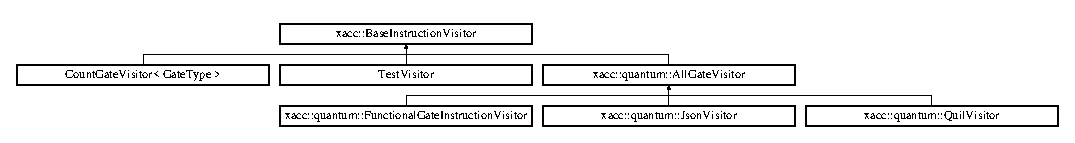
\includegraphics[height=1.478873cm]{a00016}
\end{center}
\end{figure}
\subsection*{Public Member Functions}
\begin{DoxyCompactItemize}
\item 
virtual \hyperlink{a00016_aa6f5104f5868fe1eca9be4dc4036eba4}{$\sim$\+Base\+Instruction\+Visitor} ()
\end{DoxyCompactItemize}


\subsection{Detailed Description}
The \hyperlink{a00016}{Base\+Instruction\+Visitor} is a base class for all classes that are \hyperlink{a00037}{Instruction} visitors. It basically provides a means for passing instruction visitor handles in a polymorphic manner. 

\subsection{Constructor \& Destructor Documentation}
\index{xacc\+::\+Base\+Instruction\+Visitor@{xacc\+::\+Base\+Instruction\+Visitor}!````~Base\+Instruction\+Visitor@{$\sim$\+Base\+Instruction\+Visitor}}
\index{````~Base\+Instruction\+Visitor@{$\sim$\+Base\+Instruction\+Visitor}!xacc\+::\+Base\+Instruction\+Visitor@{xacc\+::\+Base\+Instruction\+Visitor}}
\subsubsection[{\texorpdfstring{$\sim$\+Base\+Instruction\+Visitor()}{~BaseInstructionVisitor()}}]{\setlength{\rightskip}{0pt plus 5cm}virtual xacc\+::\+Base\+Instruction\+Visitor\+::$\sim$\+Base\+Instruction\+Visitor (
\begin{DoxyParamCaption}
{}
\end{DoxyParamCaption}
)\hspace{0.3cm}{\ttfamily [inline]}, {\ttfamily [virtual]}}\hypertarget{a00016_aa6f5104f5868fe1eca9be4dc4036eba4}{}\label{a00016_aa6f5104f5868fe1eca9be4dc4036eba4}
The destructor 

The documentation for this class was generated from the following file\+:\begin{DoxyCompactItemize}
\item 
Instruction\+Visitor.\+hpp\end{DoxyCompactItemize}

\hypertarget{a00017}{}\section{xacc\+:\+:Accelerator Class Reference}
\label{a00017}\index{xacc\+::\+Accelerator@{xacc\+::\+Accelerator}}


{\ttfamily \#include $<$Accelerator.\+hpp$>$}

Inheritance diagram for xacc\+:\+:Accelerator\+:\begin{figure}[H]
\begin{center}
\leavevmode
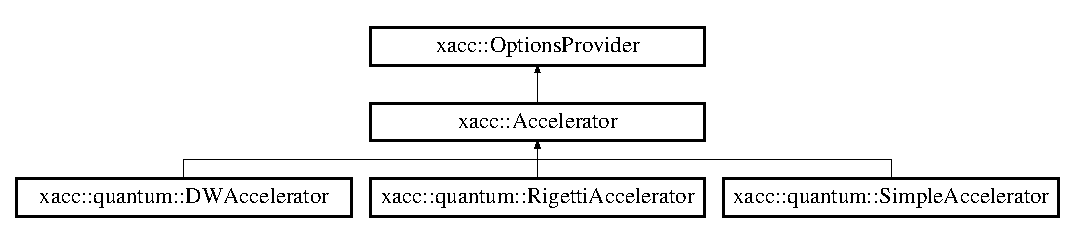
\includegraphics[height=2.679426cm]{a00017}
\end{center}
\end{figure}
\subsection*{Public Member Functions}
\begin{DoxyCompactItemize}
\item 
virtual void \hyperlink{a00017_a8cdc6f0c5a660013c29c07657a06303b}{initialize} ()=0
\item 
virtual Accelerator\+Type \hyperlink{a00017_aaffc3e4bb9880eb5041b1b58ee4c2665}{get\+Type} ()=0
\item 
virtual std\+::vector$<$ \hyperlink{a00078}{I\+R\+Transformation} $>$ \hyperlink{a00017_ad6e4a642dcb24e552675bcbeff1e1b04}{get\+I\+R\+Transformations} ()=0
\item 
virtual void \hyperlink{a00017_a89b3f3e6294f228abf03a410b0fb1674}{execute} (std\+::shared\+\_\+ptr$<$ \hyperlink{a00019}{Accelerator\+Buffer} $>$ buffer, const std\+::shared\+\_\+ptr$<$ \hyperlink{a00059}{Function} $>$ function)=0
\item 
virtual std\+::shared\+\_\+ptr$<$ \hyperlink{a00019}{Accelerator\+Buffer} $>$ \hyperlink{a00017_aab5046e8d83ab390302e0f49533e95fc}{create\+Buffer} (const std\+::string \&var\+Id)=0
\item 
virtual std\+::shared\+\_\+ptr$<$ \hyperlink{a00019}{Accelerator\+Buffer} $>$ \hyperlink{a00017_a064a2dbd58338364115c260267806945}{create\+Buffer} (const std\+::string \&var\+Id, const int size)=0
\item 
virtual std\+::shared\+\_\+ptr$<$ \hyperlink{a00019}{Accelerator\+Buffer} $>$ \hyperlink{a00017_ab3820be326e28a553fed1a824f4d41d0}{get\+Buffer} (const std\+::string \&varid)
\item 
virtual std\+::vector$<$ std\+::string $>$ \hyperlink{a00017_ae1463d7e405df89fa4af47e8922f4b82}{get\+Allocated\+Buffer\+Names} ()
\item 
virtual std\+::shared\+\_\+ptr$<$ \hyperlink{a00064}{Accelerator\+Graph} $>$ \hyperlink{a00017_adfed940ce1fa476b009344ddf5a4bbc3}{get\+Accelerator\+Connectivity} ()
\item 
virtual std\+::shared\+\_\+ptr$<$ options\+\_\+description $>$ \hyperlink{a00017_a98c9eda6b54367c75667ecfbbf167979}{get\+Options} ()
\item 
virtual \hyperlink{a00017_aed88ab0d71b765f0b0f512684ccd4b55}{$\sim$\+Accelerator} ()
\end{DoxyCompactItemize}
\subsection*{Protected Member Functions}
\begin{DoxyCompactItemize}
\item 
virtual bool \hyperlink{a00017_ae51584850faeec77299058383977ddeb}{is\+Valid\+Buffer\+Size} (const int N\+Bits)=0
\item 
void \hyperlink{a00017_ac3e781f42ec25e460174d4c41ea26b94}{store\+Buffer} (const std\+::string \&id, std\+::shared\+\_\+ptr$<$ \hyperlink{a00019}{Accelerator\+Buffer} $>$ b)
\end{DoxyCompactItemize}


\subsection{Detailed Description}
The \hyperlink{a00017}{Accelerator} class provides a high-\/level abstraction for X\+A\+CC\textquotesingle{}s interaction with attached post-\/exascale accelerators (quantum and neuromorphic processing units).

Derived Accelerators must provide a valid execute implementation that takes X\+A\+CC \hyperlink{a00077}{IR} and executes it on the attached hardware or simulator.

Derived Accelerators must provide a list of \hyperlink{a00078}{I\+R\+Transformation} instances that transform X\+A\+CC \hyperlink{a00077}{IR} to be amenable to execution on the hardware.

Derived Accelerators must provide implementations of create\+Buffer that provide a valid \hyperlink{a00019}{Accelerator\+Buffer} instance modeling the hardware memory or bits being computed on. Upon creating an \hyperlink{a00019}{Accelerator\+Buffer}, derived \hyperlink{a00017}{Accelerator} implementations must call the protected store\+Buffer method to store the \hyperlink{a00019}{Accelerator\+Buffer} for future reference by Compilers and clients of \hyperlink{a00017}{Accelerator}.

\begin{DoxyAuthor}{Author}
Alex Mc\+Caskey 
\end{DoxyAuthor}


\subsection{Constructor \& Destructor Documentation}
\index{xacc\+::\+Accelerator@{xacc\+::\+Accelerator}!````~Accelerator@{$\sim$\+Accelerator}}
\index{````~Accelerator@{$\sim$\+Accelerator}!xacc\+::\+Accelerator@{xacc\+::\+Accelerator}}
\subsubsection[{\texorpdfstring{$\sim$\+Accelerator()}{~Accelerator()}}]{\setlength{\rightskip}{0pt plus 5cm}virtual xacc\+::\+Accelerator\+::$\sim$\+Accelerator (
\begin{DoxyParamCaption}
{}
\end{DoxyParamCaption}
)\hspace{0.3cm}{\ttfamily [inline]}, {\ttfamily [virtual]}}\hypertarget{a00017_aed88ab0d71b765f0b0f512684ccd4b55}{}\label{a00017_aed88ab0d71b765f0b0f512684ccd4b55}
Destructor 

\subsection{Member Function Documentation}
\index{xacc\+::\+Accelerator@{xacc\+::\+Accelerator}!create\+Buffer@{create\+Buffer}}
\index{create\+Buffer@{create\+Buffer}!xacc\+::\+Accelerator@{xacc\+::\+Accelerator}}
\subsubsection[{\texorpdfstring{create\+Buffer(const std\+::string \&var\+Id)=0}{createBuffer(const std::string \&varId)=0}}]{\setlength{\rightskip}{0pt plus 5cm}virtual std\+::shared\+\_\+ptr$<${\bf Accelerator\+Buffer}$>$ xacc\+::\+Accelerator\+::create\+Buffer (
\begin{DoxyParamCaption}
\item[{const std\+::string \&}]{var\+Id}
\end{DoxyParamCaption}
)\hspace{0.3cm}{\ttfamily [pure virtual]}}\hypertarget{a00017_aab5046e8d83ab390302e0f49533e95fc}{}\label{a00017_aab5046e8d83ab390302e0f49533e95fc}
Create, store, and return an \hyperlink{a00019}{Accelerator\+Buffer} with the given variable id string. This method returns all available qubits for this \hyperlink{a00017}{Accelerator}. The string id serves as a unique identifier for future lookups and reuse of the \hyperlink{a00019}{Accelerator\+Buffer}.


\begin{DoxyParams}{Parameters}
{\em var\+Id} & The variable name of the created buffer \\
\hline
\end{DoxyParams}
\begin{DoxyReturn}{Returns}
buffer The buffer instance created. 
\end{DoxyReturn}


Implemented in \hyperlink{a00042_add60637a4b3c055e7f2ffa3bf8e320ac}{xacc\+::quantum\+::\+D\+W\+Accelerator}, \hyperlink{a00123_a46445d77d4b8ad2689571d0db6604380}{xacc\+::quantum\+::\+Simple\+Accelerator}, and \hyperlink{a00112_ada3ceb986e51ab5aa721f2a08e083cd6}{xacc\+::quantum\+::\+Rigetti\+Accelerator}.

\index{xacc\+::\+Accelerator@{xacc\+::\+Accelerator}!create\+Buffer@{create\+Buffer}}
\index{create\+Buffer@{create\+Buffer}!xacc\+::\+Accelerator@{xacc\+::\+Accelerator}}
\subsubsection[{\texorpdfstring{create\+Buffer(const std\+::string \&var\+Id, const int size)=0}{createBuffer(const std::string \&varId, const int size)=0}}]{\setlength{\rightskip}{0pt plus 5cm}virtual std\+::shared\+\_\+ptr$<${\bf Accelerator\+Buffer}$>$ xacc\+::\+Accelerator\+::create\+Buffer (
\begin{DoxyParamCaption}
\item[{const std\+::string \&}]{var\+Id, }
\item[{const int}]{size}
\end{DoxyParamCaption}
)\hspace{0.3cm}{\ttfamily [pure virtual]}}\hypertarget{a00017_a064a2dbd58338364115c260267806945}{}\label{a00017_a064a2dbd58338364115c260267806945}
Create, store, and return an \hyperlink{a00019}{Accelerator\+Buffer} with the given variable id string and of the given number of bits. The string id serves as a unique identifier for future lookups and reuse of the \hyperlink{a00019}{Accelerator\+Buffer}.


\begin{DoxyParams}{Parameters}
{\em var\+Id} & The variable name of the created buffer \\
\hline
{\em size} & The number of bits in the created buffer \\
\hline
\end{DoxyParams}
\begin{DoxyReturn}{Returns}
buffer The buffer instance created. 
\end{DoxyReturn}


Implemented in \hyperlink{a00042_a718d7cb51a35e694d960385e1ea2f99f}{xacc\+::quantum\+::\+D\+W\+Accelerator}, \hyperlink{a00112_a731551c94b1abef40d2cf032e8712df6}{xacc\+::quantum\+::\+Rigetti\+Accelerator}, and \hyperlink{a00123_adb9393692e9f484df241aa5d014030d1}{xacc\+::quantum\+::\+Simple\+Accelerator}.

\index{xacc\+::\+Accelerator@{xacc\+::\+Accelerator}!execute@{execute}}
\index{execute@{execute}!xacc\+::\+Accelerator@{xacc\+::\+Accelerator}}
\subsubsection[{\texorpdfstring{execute(std\+::shared\+\_\+ptr$<$ Accelerator\+Buffer $>$ buffer, const std\+::shared\+\_\+ptr$<$ Function $>$ function)=0}{execute(std::shared\_ptr< AcceleratorBuffer > buffer, const std::shared\_ptr< Function > function)=0}}]{\setlength{\rightskip}{0pt plus 5cm}virtual void xacc\+::\+Accelerator\+::execute (
\begin{DoxyParamCaption}
\item[{std\+::shared\+\_\+ptr$<$ {\bf Accelerator\+Buffer} $>$}]{buffer, }
\item[{const std\+::shared\+\_\+ptr$<$ {\bf Function} $>$}]{function}
\end{DoxyParamCaption}
)\hspace{0.3cm}{\ttfamily [pure virtual]}}\hypertarget{a00017_a89b3f3e6294f228abf03a410b0fb1674}{}\label{a00017_a89b3f3e6294f228abf03a410b0fb1674}
Execute the provided X\+A\+CC \hyperlink{a00077}{IR} \hyperlink{a00059}{Function} on the provided \hyperlink{a00019}{Accelerator\+Buffer}.


\begin{DoxyParams}{Parameters}
{\em buffer} & The buffer of bits this \hyperlink{a00017}{Accelerator} should operate on. \\
\hline
{\em function} & The kernel to execute. \\
\hline
\end{DoxyParams}
\index{xacc\+::\+Accelerator@{xacc\+::\+Accelerator}!get\+Accelerator\+Connectivity@{get\+Accelerator\+Connectivity}}
\index{get\+Accelerator\+Connectivity@{get\+Accelerator\+Connectivity}!xacc\+::\+Accelerator@{xacc\+::\+Accelerator}}
\subsubsection[{\texorpdfstring{get\+Accelerator\+Connectivity()}{getAcceleratorConnectivity()}}]{\setlength{\rightskip}{0pt plus 5cm}virtual std\+::shared\+\_\+ptr$<${\bf Accelerator\+Graph}$>$ xacc\+::\+Accelerator\+::get\+Accelerator\+Connectivity (
\begin{DoxyParamCaption}
{}
\end{DoxyParamCaption}
)\hspace{0.3cm}{\ttfamily [inline]}, {\ttfamily [virtual]}}\hypertarget{a00017_adfed940ce1fa476b009344ddf5a4bbc3}{}\label{a00017_adfed940ce1fa476b009344ddf5a4bbc3}
Return the graph structure for this \hyperlink{a00017}{Accelerator}.

\begin{DoxyReturn}{Returns}
connectivity\+Graph The graph structure of this \hyperlink{a00017}{Accelerator} 
\end{DoxyReturn}


Reimplemented in \hyperlink{a00042_a006afa60749790681fc76beddc254926}{xacc\+::quantum\+::\+D\+W\+Accelerator}.

\index{xacc\+::\+Accelerator@{xacc\+::\+Accelerator}!get\+Allocated\+Buffer\+Names@{get\+Allocated\+Buffer\+Names}}
\index{get\+Allocated\+Buffer\+Names@{get\+Allocated\+Buffer\+Names}!xacc\+::\+Accelerator@{xacc\+::\+Accelerator}}
\subsubsection[{\texorpdfstring{get\+Allocated\+Buffer\+Names()}{getAllocatedBufferNames()}}]{\setlength{\rightskip}{0pt plus 5cm}virtual std\+::vector$<$std\+::string$>$ xacc\+::\+Accelerator\+::get\+Allocated\+Buffer\+Names (
\begin{DoxyParamCaption}
{}
\end{DoxyParamCaption}
)\hspace{0.3cm}{\ttfamily [inline]}, {\ttfamily [virtual]}}\hypertarget{a00017_ae1463d7e405df89fa4af47e8922f4b82}{}\label{a00017_ae1463d7e405df89fa4af47e8922f4b82}
Return all allocated \hyperlink{a00019}{Accelerator\+Buffer} variable names.

\begin{DoxyReturn}{Returns}
var\+Names The buffer variable names 
\end{DoxyReturn}
\index{xacc\+::\+Accelerator@{xacc\+::\+Accelerator}!get\+Buffer@{get\+Buffer}}
\index{get\+Buffer@{get\+Buffer}!xacc\+::\+Accelerator@{xacc\+::\+Accelerator}}
\subsubsection[{\texorpdfstring{get\+Buffer(const std\+::string \&varid)}{getBuffer(const std::string \&varid)}}]{\setlength{\rightskip}{0pt plus 5cm}virtual std\+::shared\+\_\+ptr$<${\bf Accelerator\+Buffer}$>$ xacc\+::\+Accelerator\+::get\+Buffer (
\begin{DoxyParamCaption}
\item[{const std\+::string \&}]{varid}
\end{DoxyParamCaption}
)\hspace{0.3cm}{\ttfamily [inline]}, {\ttfamily [virtual]}}\hypertarget{a00017_ab3820be326e28a553fed1a824f4d41d0}{}\label{a00017_ab3820be326e28a553fed1a824f4d41d0}
Return the stored \hyperlink{a00019}{Accelerator\+Buffer} with the provided string id.


\begin{DoxyParams}{Parameters}
{\em varid} & The variable name of the created buffer \\
\hline
\end{DoxyParams}
\begin{DoxyReturn}{Returns}
buffer The buffer with given varid. 
\end{DoxyReturn}
\index{xacc\+::\+Accelerator@{xacc\+::\+Accelerator}!get\+I\+R\+Transformations@{get\+I\+R\+Transformations}}
\index{get\+I\+R\+Transformations@{get\+I\+R\+Transformations}!xacc\+::\+Accelerator@{xacc\+::\+Accelerator}}
\subsubsection[{\texorpdfstring{get\+I\+R\+Transformations()=0}{getIRTransformations()=0}}]{\setlength{\rightskip}{0pt plus 5cm}virtual std\+::vector$<${\bf I\+R\+Transformation}$>$ xacc\+::\+Accelerator\+::get\+I\+R\+Transformations (
\begin{DoxyParamCaption}
{}
\end{DoxyParamCaption}
)\hspace{0.3cm}{\ttfamily [pure virtual]}}\hypertarget{a00017_ad6e4a642dcb24e552675bcbeff1e1b04}{}\label{a00017_ad6e4a642dcb24e552675bcbeff1e1b04}
Return any \hyperlink{a00077}{IR} Transformations that must be applied to ensure the compiled \hyperlink{a00077}{IR} is amenable to execution on this \hyperlink{a00017}{Accelerator}.

\begin{DoxyReturn}{Returns}
transformations The \hyperlink{a00077}{IR} transformations this \hyperlink{a00017}{Accelerator} exposes 
\end{DoxyReturn}


Implemented in \hyperlink{a00042_a89da20bd079a22d6581ea2da2293b973}{xacc\+::quantum\+::\+D\+W\+Accelerator}, \hyperlink{a00112_a443683a1dfb000603c640b2ee303cf66}{xacc\+::quantum\+::\+Rigetti\+Accelerator}, and \hyperlink{a00123_afc49c9e7973ba6c6ff9761c36198323d}{xacc\+::quantum\+::\+Simple\+Accelerator}.

\index{xacc\+::\+Accelerator@{xacc\+::\+Accelerator}!get\+Options@{get\+Options}}
\index{get\+Options@{get\+Options}!xacc\+::\+Accelerator@{xacc\+::\+Accelerator}}
\subsubsection[{\texorpdfstring{get\+Options()}{getOptions()}}]{\setlength{\rightskip}{0pt plus 5cm}virtual std\+::shared\+\_\+ptr$<$options\+\_\+description$>$ xacc\+::\+Accelerator\+::get\+Options (
\begin{DoxyParamCaption}
{}
\end{DoxyParamCaption}
)\hspace{0.3cm}{\ttfamily [inline]}, {\ttfamily [virtual]}}\hypertarget{a00017_a98c9eda6b54367c75667ecfbbf167979}{}\label{a00017_a98c9eda6b54367c75667ecfbbf167979}
Return an empty options\+\_\+description, this is for subclasses to implement. 

Implements \hyperlink{a00091_a6d150954f852109bfe2c1ae90222926f}{xacc\+::\+Options\+Provider}.



Reimplemented in \hyperlink{a00042_a09926db9f99706307ae6ce5b56845bca}{xacc\+::quantum\+::\+D\+W\+Accelerator}, and \hyperlink{a00112_a9ee9e62aecbccf193894ca3388676f9f}{xacc\+::quantum\+::\+Rigetti\+Accelerator}.

\index{xacc\+::\+Accelerator@{xacc\+::\+Accelerator}!get\+Type@{get\+Type}}
\index{get\+Type@{get\+Type}!xacc\+::\+Accelerator@{xacc\+::\+Accelerator}}
\subsubsection[{\texorpdfstring{get\+Type()=0}{getType()=0}}]{\setlength{\rightskip}{0pt plus 5cm}virtual Accelerator\+Type xacc\+::\+Accelerator\+::get\+Type (
\begin{DoxyParamCaption}
{}
\end{DoxyParamCaption}
)\hspace{0.3cm}{\ttfamily [pure virtual]}}\hypertarget{a00017_aaffc3e4bb9880eb5041b1b58ee4c2665}{}\label{a00017_aaffc3e4bb9880eb5041b1b58ee4c2665}
Return the type of this \hyperlink{a00017}{Accelerator}.

\begin{DoxyReturn}{Returns}
type The \hyperlink{a00017}{Accelerator} type -\/ Gate or A\+QC Q\+PU, or N\+PU 
\end{DoxyReturn}


Implemented in \hyperlink{a00042_abe50e427b4bec0460cc238405cb569f9}{xacc\+::quantum\+::\+D\+W\+Accelerator}, \hyperlink{a00112_aab0d4674da5273d55407b9ab77cde890}{xacc\+::quantum\+::\+Rigetti\+Accelerator}, and \hyperlink{a00123_ad76eeb0bbd7de21aad5bd20d20970a98}{xacc\+::quantum\+::\+Simple\+Accelerator}.

\index{xacc\+::\+Accelerator@{xacc\+::\+Accelerator}!initialize@{initialize}}
\index{initialize@{initialize}!xacc\+::\+Accelerator@{xacc\+::\+Accelerator}}
\subsubsection[{\texorpdfstring{initialize()=0}{initialize()=0}}]{\setlength{\rightskip}{0pt plus 5cm}virtual void xacc\+::\+Accelerator\+::initialize (
\begin{DoxyParamCaption}
{}
\end{DoxyParamCaption}
)\hspace{0.3cm}{\ttfamily [pure virtual]}}\hypertarget{a00017_a8cdc6f0c5a660013c29c07657a06303b}{}\label{a00017_a8cdc6f0c5a660013c29c07657a06303b}
Initialize this \hyperlink{a00017}{Accelerator}. This method is called by the X\+A\+CC framework after an \hyperlink{a00017}{Accelerator} has been requested and created. Perform any work you need done before execution here. 

Implemented in \hyperlink{a00042_acaefd5747409f31cf5c3e42d98475ce2}{xacc\+::quantum\+::\+D\+W\+Accelerator}, \hyperlink{a00112_ab8b6af9bb9dcb110201e9ee5cac74b4f}{xacc\+::quantum\+::\+Rigetti\+Accelerator}, and \hyperlink{a00123_a392e3b30523f5f681127e7e98887108c}{xacc\+::quantum\+::\+Simple\+Accelerator}.

\index{xacc\+::\+Accelerator@{xacc\+::\+Accelerator}!is\+Valid\+Buffer\+Size@{is\+Valid\+Buffer\+Size}}
\index{is\+Valid\+Buffer\+Size@{is\+Valid\+Buffer\+Size}!xacc\+::\+Accelerator@{xacc\+::\+Accelerator}}
\subsubsection[{\texorpdfstring{is\+Valid\+Buffer\+Size(const int N\+Bits)=0}{isValidBufferSize(const int NBits)=0}}]{\setlength{\rightskip}{0pt plus 5cm}virtual bool xacc\+::\+Accelerator\+::is\+Valid\+Buffer\+Size (
\begin{DoxyParamCaption}
\item[{const int}]{N\+Bits}
\end{DoxyParamCaption}
)\hspace{0.3cm}{\ttfamily [protected]}, {\ttfamily [pure virtual]}}\hypertarget{a00017_ae51584850faeec77299058383977ddeb}{}\label{a00017_ae51584850faeec77299058383977ddeb}
Return true if this \hyperlink{a00017}{Accelerator} can allocated N\+Bits number of bits. This is meant to be implemented and used by subclasses.


\begin{DoxyParams}{Parameters}
{\em N\+Bits} & The number of bits to allocate \\
\hline
\end{DoxyParams}
\begin{DoxyReturn}{Returns}
valid True if size is valid. 
\end{DoxyReturn}


Implemented in \hyperlink{a00042_a4c2ee30212a919d8ddf7f9555df25195}{xacc\+::quantum\+::\+D\+W\+Accelerator}, \hyperlink{a00123_a60b9db2d6aed235857c45413a070338e}{xacc\+::quantum\+::\+Simple\+Accelerator}, and \hyperlink{a00112_a61352c07062597aad2393fbeed4cc025}{xacc\+::quantum\+::\+Rigetti\+Accelerator}.

\index{xacc\+::\+Accelerator@{xacc\+::\+Accelerator}!store\+Buffer@{store\+Buffer}}
\index{store\+Buffer@{store\+Buffer}!xacc\+::\+Accelerator@{xacc\+::\+Accelerator}}
\subsubsection[{\texorpdfstring{store\+Buffer(const std\+::string \&id, std\+::shared\+\_\+ptr$<$ Accelerator\+Buffer $>$ b)}{storeBuffer(const std::string \&id, std::shared\_ptr< AcceleratorBuffer > b)}}]{\setlength{\rightskip}{0pt plus 5cm}void xacc\+::\+Accelerator\+::store\+Buffer (
\begin{DoxyParamCaption}
\item[{const std\+::string \&}]{id, }
\item[{std\+::shared\+\_\+ptr$<$ {\bf Accelerator\+Buffer} $>$}]{b}
\end{DoxyParamCaption}
)\hspace{0.3cm}{\ttfamily [inline]}, {\ttfamily [protected]}}\hypertarget{a00017_ac3e781f42ec25e460174d4c41ea26b94}{}\label{a00017_ac3e781f42ec25e460174d4c41ea26b94}
This protected method is to be used by derived Accelerators to store any created \hyperlink{a00019}{Accelerator\+Buffer}.


\begin{DoxyParams}{Parameters}
{\em id} & The variable name of the buffer to store \\
\hline
{\em b} & The buffer to store \\
\hline
\end{DoxyParams}


The documentation for this class was generated from the following file\+:\begin{DoxyCompactItemize}
\item 
Accelerator.\+hpp\end{DoxyCompactItemize}

\hypertarget{a00018}{}\section{xacc\+:\+:Base\+Instruction\+Visitor Class Reference}
\label{a00018}\index{xacc\+::\+Base\+Instruction\+Visitor@{xacc\+::\+Base\+Instruction\+Visitor}}


{\ttfamily \#include $<$Instruction\+Visitor.\+hpp$>$}

Inheritance diagram for xacc\+:\+:Base\+Instruction\+Visitor\+:\begin{figure}[H]
\begin{center}
\leavevmode
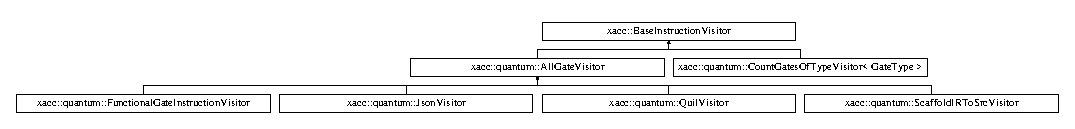
\includegraphics[height=1.288344cm]{a00018}
\end{center}
\end{figure}
\subsection*{Public Member Functions}
\begin{DoxyCompactItemize}
\item 
virtual \hyperlink{a00018_aa6f5104f5868fe1eca9be4dc4036eba4}{$\sim$\+Base\+Instruction\+Visitor} ()
\end{DoxyCompactItemize}


\subsection{Detailed Description}
The \hyperlink{a00018}{Base\+Instruction\+Visitor} is a base class for all classes that are \hyperlink{a00046}{Instruction} visitors. It basically provides a means for passing instruction visitor handles in a polymorphic manner. 

\subsection{Constructor \& Destructor Documentation}
\index{xacc\+::\+Base\+Instruction\+Visitor@{xacc\+::\+Base\+Instruction\+Visitor}!````~Base\+Instruction\+Visitor@{$\sim$\+Base\+Instruction\+Visitor}}
\index{````~Base\+Instruction\+Visitor@{$\sim$\+Base\+Instruction\+Visitor}!xacc\+::\+Base\+Instruction\+Visitor@{xacc\+::\+Base\+Instruction\+Visitor}}
\subsubsection[{\texorpdfstring{$\sim$\+Base\+Instruction\+Visitor()}{~BaseInstructionVisitor()}}]{\setlength{\rightskip}{0pt plus 5cm}virtual xacc\+::\+Base\+Instruction\+Visitor\+::$\sim$\+Base\+Instruction\+Visitor (
\begin{DoxyParamCaption}
{}
\end{DoxyParamCaption}
)\hspace{0.3cm}{\ttfamily [inline]}, {\ttfamily [virtual]}}\hypertarget{a00018_aa6f5104f5868fe1eca9be4dc4036eba4}{}\label{a00018_aa6f5104f5868fe1eca9be4dc4036eba4}
The destructor 

The documentation for this class was generated from the following file\+:\begin{DoxyCompactItemize}
\item 
Instruction\+Visitor.\+hpp\end{DoxyCompactItemize}

\hypertarget{a00019}{}\section{xacc\+:\+:Accelerator\+Buffer Class Reference}
\label{a00019}\index{xacc\+::\+Accelerator\+Buffer@{xacc\+::\+Accelerator\+Buffer}}


{\ttfamily \#include $<$Accelerator\+Buffer.\+hpp$>$}

Inheritance diagram for xacc\+:\+:Accelerator\+Buffer\+:\begin{figure}[H]
\begin{center}
\leavevmode
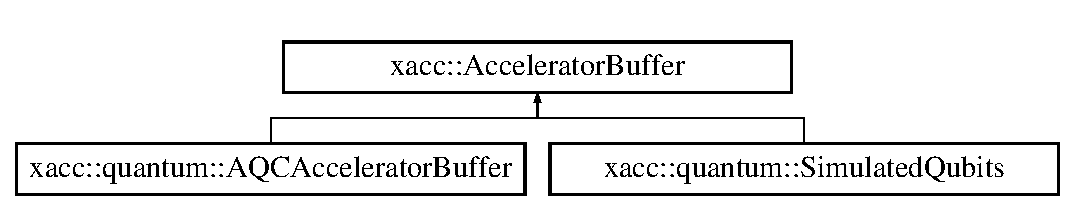
\includegraphics[height=2.000000cm]{a00019}
\end{center}
\end{figure}
\subsection*{Public Member Functions}
\begin{DoxyCompactItemize}
\item 
\hyperlink{a00019_ab606d8af942120d60b51a4fffcd75c98}{Accelerator\+Buffer} (const std\+::string \&str, const int N)
\item 
{\footnotesize template$<$typename... Indices$>$ }\\{\bfseries Accelerator\+Buffer} (const std\+::string \&str, int first\+Index, Indices...\+indices)\hypertarget{a00019_ac550d89390562095c56aa1b14ae85001}{}\label{a00019_ac550d89390562095c56aa1b14ae85001}

\item 
int {\bfseries size} ()\hypertarget{a00019_aa2a3101c2e3ae3550172bf49f9587f3b}{}\label{a00019_aa2a3101c2e3ae3550172bf49f9587f3b}

\item 
std\+::string {\bfseries name} ()\hypertarget{a00019_ad5b646e9efc21b6d0bcc22cd6f649c22}{}\label{a00019_ad5b646e9efc21b6d0bcc22cd6f649c22}

\item 
void {\bfseries reset\+Buffer} ()\hypertarget{a00019_aa6d6e9cfee6170333c1f03507345743f}{}\label{a00019_aa6d6e9cfee6170333c1f03507345743f}

\item 
void {\bfseries update\+Bit} (const int idx, int zero\+Or\+One)\hypertarget{a00019_a4bc0edbe9aa0d463f67ddcc38265066f}{}\label{a00019_a4bc0edbe9aa0d463f67ddcc38265066f}

\item 
void {\bfseries append\+Measurement} (const boost\+::dynamic\+\_\+bitset$<$$>$ \&measurement)\hypertarget{a00019_ac161c4f984f774d08197871094aabc67}{}\label{a00019_ac161c4f984f774d08197871094aabc67}

\item 
double {\bfseries get\+Average} () const \hypertarget{a00019_a97cf3cc4e1aaa8ac3cee7817860f77c1}{}\label{a00019_a97cf3cc4e1aaa8ac3cee7817860f77c1}

\item 
Accelerator\+Bit\+State {\bfseries get\+Accelerator\+Bit\+State} (const int idx)\hypertarget{a00019_aba6ef359f3117faa98f0eb8da90d909e}{}\label{a00019_aba6ef359f3117faa98f0eb8da90d909e}

\item 
virtual void {\bfseries print} ()\hypertarget{a00019_add0835e188f0eda4f1b68a28ddc79786}{}\label{a00019_add0835e188f0eda4f1b68a28ddc79786}

\item 
virtual void {\bfseries print} (std\+::ostream \&stream)\hypertarget{a00019_a7c59462451223772b41ef232b06a7dfa}{}\label{a00019_a7c59462451223772b41ef232b06a7dfa}

\end{DoxyCompactItemize}
\subsection*{Protected Attributes}
\begin{DoxyCompactItemize}
\item 
std\+::vector$<$ boost\+::dynamic\+\_\+bitset$<$$>$ $>$ {\bfseries measurements}\hypertarget{a00019_a5464b23a964985df2547f657877c9ea5}{}\label{a00019_a5464b23a964985df2547f657877c9ea5}

\item 
std\+::string {\bfseries buffer\+Id}\hypertarget{a00019_a3198e034d07d9b77b62da03e6592a221}{}\label{a00019_a3198e034d07d9b77b62da03e6592a221}

\item 
std\+::vector$<$ \hyperlink{a00018}{Accelerator\+Bit} $>$ {\bfseries bits}\hypertarget{a00019_ab6dbb8c22f8adc6aba34b00a84066854}{}\label{a00019_ab6dbb8c22f8adc6aba34b00a84066854}

\end{DoxyCompactItemize}


\subsection{Detailed Description}
The \hyperlink{a00019}{Accelerator\+Buffer} models an allocated buffer of bits that are operated on by a kernel. As such, the \hyperlink{a00019}{Accelerator\+Buffer}\textquotesingle{}s primary role is to store \hyperlink{a00017}{Accelerator} execution results.

\begin{DoxyAuthor}{Author}
Alex Mc\+Caskey 
\end{DoxyAuthor}


\subsection{Constructor \& Destructor Documentation}
\index{xacc\+::\+Accelerator\+Buffer@{xacc\+::\+Accelerator\+Buffer}!Accelerator\+Buffer@{Accelerator\+Buffer}}
\index{Accelerator\+Buffer@{Accelerator\+Buffer}!xacc\+::\+Accelerator\+Buffer@{xacc\+::\+Accelerator\+Buffer}}
\subsubsection[{\texorpdfstring{Accelerator\+Buffer(const std\+::string \&str, const int N)}{AcceleratorBuffer(const std::string \&str, const int N)}}]{\setlength{\rightskip}{0pt plus 5cm}xacc\+::\+Accelerator\+Buffer\+::\+Accelerator\+Buffer (
\begin{DoxyParamCaption}
\item[{const std\+::string \&}]{str, }
\item[{const int}]{N}
\end{DoxyParamCaption}
)\hspace{0.3cm}{\ttfamily [inline]}}\hypertarget{a00019_ab606d8af942120d60b51a4fffcd75c98}{}\label{a00019_ab606d8af942120d60b51a4fffcd75c98}
The Constructor 

The documentation for this class was generated from the following file\+:\begin{DoxyCompactItemize}
\item 
Accelerator\+Buffer.\+hpp\end{DoxyCompactItemize}

\hypertarget{a00020}{}\section{xacc\+:\+:Compiler Class Reference}
\label{a00020}\index{xacc\+::\+Compiler@{xacc\+::\+Compiler}}


{\ttfamily \#include $<$Compiler.\+hpp$>$}

Inheritance diagram for xacc\+:\+:Compiler\+:\begin{figure}[H]
\begin{center}
\leavevmode
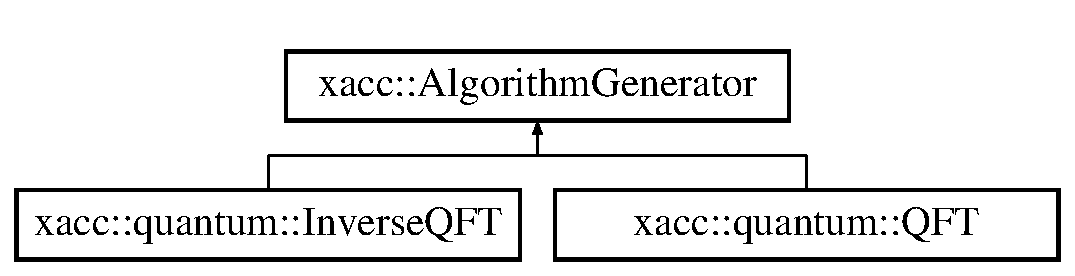
\includegraphics[height=2.772277cm]{a00020}
\end{center}
\end{figure}
\subsection*{Public Member Functions}
\begin{DoxyCompactItemize}
\item 
virtual std\+::shared\+\_\+ptr$<$ \hyperlink{a00041}{IR} $>$ \hyperlink{a00020_a546a40c95bb93af6a0c0ac48dbeaffc8}{compile} (const std\+::string \&src, std\+::shared\+\_\+ptr$<$ \hyperlink{a00011}{Accelerator} $>$ acc)=0
\item 
virtual std\+::shared\+\_\+ptr$<$ \hyperlink{a00041}{IR} $>$ \hyperlink{a00020_a9092f5f779b570c91569b59621280c04}{compile} (const std\+::string \&src)=0
\item 
virtual const std\+::string \hyperlink{a00020_a87fca9100e6462122f5b687c3a0fb3fb}{get\+Name} ()=0
\item 
virtual std\+::shared\+\_\+ptr$<$ options\+\_\+description $>$ \hyperlink{a00020_a9f5a8965c9c2dd895016d18264ebbe92}{get\+Options} ()
\item 
virtual \hyperlink{a00020_a5d0b012687d9b44893872eaa81e47b38}{$\sim$\+Compiler} ()
\end{DoxyCompactItemize}
\subsection*{Protected Attributes}
\begin{DoxyCompactItemize}
\item 
std\+::string \hyperlink{a00020_a0ad81c816c09e5113d03cdc02165c453}{kernel\+Source}
\item 
std\+::shared\+\_\+ptr$<$ \hyperlink{a00011}{Accelerator} $>$ \hyperlink{a00020_ad4cbb467fa7e377bac6c054ffcb22b7c}{accelerator}
\end{DoxyCompactItemize}


\subsection{Detailed Description}
The \hyperlink{a00020}{Compiler} class provides an extensible interface for injecting custom compilation mechanisms into the X\+A\+CC framework. Implementations provide a compile method that takes the kernel source code string, performs compiler-\/specific compilation mechanism, and returns a valid X\+A\+CC \hyperlink{a00041}{IR} instance modeling the result of the compilation. 

\subsection{Constructor \& Destructor Documentation}
\index{xacc\+::\+Compiler@{xacc\+::\+Compiler}!````~Compiler@{$\sim$\+Compiler}}
\index{````~Compiler@{$\sim$\+Compiler}!xacc\+::\+Compiler@{xacc\+::\+Compiler}}
\subsubsection[{\texorpdfstring{$\sim$\+Compiler()}{~Compiler()}}]{\setlength{\rightskip}{0pt plus 5cm}virtual xacc\+::\+Compiler\+::$\sim$\+Compiler (
\begin{DoxyParamCaption}
{}
\end{DoxyParamCaption}
)\hspace{0.3cm}{\ttfamily [inline]}, {\ttfamily [virtual]}}\hypertarget{a00020_a5d0b012687d9b44893872eaa81e47b38}{}\label{a00020_a5d0b012687d9b44893872eaa81e47b38}
The destructor 

\subsection{Member Function Documentation}
\index{xacc\+::\+Compiler@{xacc\+::\+Compiler}!compile@{compile}}
\index{compile@{compile}!xacc\+::\+Compiler@{xacc\+::\+Compiler}}
\subsubsection[{\texorpdfstring{compile(const std\+::string \&src, std\+::shared\+\_\+ptr$<$ Accelerator $>$ acc)=0}{compile(const std::string \&src, std::shared\_ptr< Accelerator > acc)=0}}]{\setlength{\rightskip}{0pt plus 5cm}virtual std\+::shared\+\_\+ptr$<${\bf IR}$>$ xacc\+::\+Compiler\+::compile (
\begin{DoxyParamCaption}
\item[{const std\+::string \&}]{src, }
\item[{std\+::shared\+\_\+ptr$<$ {\bf Accelerator} $>$}]{acc}
\end{DoxyParamCaption}
)\hspace{0.3cm}{\ttfamily [pure virtual]}}\hypertarget{a00020_a546a40c95bb93af6a0c0ac48dbeaffc8}{}\label{a00020_a546a40c95bb93af6a0c0ac48dbeaffc8}
This method is to be implemented by derived Compilers and is in charge of executing the compilation mechanism on the provided source string. Implementations also are given access to the \hyperlink{a00011}{Accelerator} that this source code is intended for.


\begin{DoxyParams}{Parameters}
{\em src} & The kernel source string. \\
\hline
{\em acc} & The \hyperlink{a00011}{Accelerator} this code will be executed on \\
\hline
\end{DoxyParams}
\begin{DoxyReturn}{Returns}
ir Intermediate representation for provided source kernel code. 
\end{DoxyReturn}


Implemented in \hyperlink{a00065_a7caede75bb2304ba405966651b115543}{xacc\+::quantum\+::\+Scaffold\+Compiler}, \hyperlink{a00050_a2421482415ca4e09963ea4ecddff8100}{xacc\+::quantum\+::\+Quil\+Compiler}, and \hyperlink{a00024_a0f7f6b10b4a881cb27b36eaa6d39e7b1}{xacc\+::quantum\+::\+D\+Wave\+Compiler}.

\index{xacc\+::\+Compiler@{xacc\+::\+Compiler}!compile@{compile}}
\index{compile@{compile}!xacc\+::\+Compiler@{xacc\+::\+Compiler}}
\subsubsection[{\texorpdfstring{compile(const std\+::string \&src)=0}{compile(const std::string \&src)=0}}]{\setlength{\rightskip}{0pt plus 5cm}virtual std\+::shared\+\_\+ptr$<${\bf IR}$>$ xacc\+::\+Compiler\+::compile (
\begin{DoxyParamCaption}
\item[{const std\+::string \&}]{src}
\end{DoxyParamCaption}
)\hspace{0.3cm}{\ttfamily [pure virtual]}}\hypertarget{a00020_a9092f5f779b570c91569b59621280c04}{}\label{a00020_a9092f5f779b570c91569b59621280c04}
This method is to be implemented by derived Compilers and is in charge of executing the compilation mechanism on the provided source string. 
\begin{DoxyParams}{Parameters}
{\em src} & \\
\hline
\end{DoxyParams}
\begin{DoxyReturn}{Returns}

\end{DoxyReturn}


Implemented in \hyperlink{a00065_a3736ecc229fe6acdd4c991e85d7a1f08}{xacc\+::quantum\+::\+Scaffold\+Compiler}, \hyperlink{a00050_adf4d321ecb0df3fa7728999f941c83b2}{xacc\+::quantum\+::\+Quil\+Compiler}, and \hyperlink{a00024_a893e1d1c81a8aaf6e2435c9bceab575e}{xacc\+::quantum\+::\+D\+Wave\+Compiler}.

\index{xacc\+::\+Compiler@{xacc\+::\+Compiler}!get\+Name@{get\+Name}}
\index{get\+Name@{get\+Name}!xacc\+::\+Compiler@{xacc\+::\+Compiler}}
\subsubsection[{\texorpdfstring{get\+Name()=0}{getName()=0}}]{\setlength{\rightskip}{0pt plus 5cm}virtual const std\+::string xacc\+::\+Compiler\+::get\+Name (
\begin{DoxyParamCaption}
{}
\end{DoxyParamCaption}
)\hspace{0.3cm}{\ttfamily [pure virtual]}}\hypertarget{a00020_a87fca9100e6462122f5b687c3a0fb3fb}{}\label{a00020_a87fca9100e6462122f5b687c3a0fb3fb}
Return the name of this \hyperlink{a00020}{Compiler} \begin{DoxyReturn}{Returns}
name \hyperlink{a00020}{Compiler} name 
\end{DoxyReturn}


Implemented in \hyperlink{a00065_a3f537054a3924a1d14f4ceb0f0181161}{xacc\+::quantum\+::\+Scaffold\+Compiler}, \hyperlink{a00050_ae7d52140b6dd52730edc6e38ae48f437}{xacc\+::quantum\+::\+Quil\+Compiler}, and \hyperlink{a00024_a8a180031ae563e1a9aac611e8066c181}{xacc\+::quantum\+::\+D\+Wave\+Compiler}.

\index{xacc\+::\+Compiler@{xacc\+::\+Compiler}!get\+Options@{get\+Options}}
\index{get\+Options@{get\+Options}!xacc\+::\+Compiler@{xacc\+::\+Compiler}}
\subsubsection[{\texorpdfstring{get\+Options()}{getOptions()}}]{\setlength{\rightskip}{0pt plus 5cm}virtual std\+::shared\+\_\+ptr$<$options\+\_\+description$>$ xacc\+::\+Compiler\+::get\+Options (
\begin{DoxyParamCaption}
{}
\end{DoxyParamCaption}
)\hspace{0.3cm}{\ttfamily [inline]}, {\ttfamily [virtual]}}\hypertarget{a00020_a9f5a8965c9c2dd895016d18264ebbe92}{}\label{a00020_a9f5a8965c9c2dd895016d18264ebbe92}
Return an empty options\+\_\+description, this is for subclasses to implement. 

Implements \hyperlink{a00046_a6d150954f852109bfe2c1ae90222926f}{xacc\+::\+Options\+Provider}.



\subsection{Member Data Documentation}
\index{xacc\+::\+Compiler@{xacc\+::\+Compiler}!accelerator@{accelerator}}
\index{accelerator@{accelerator}!xacc\+::\+Compiler@{xacc\+::\+Compiler}}
\subsubsection[{\texorpdfstring{accelerator}{accelerator}}]{\setlength{\rightskip}{0pt plus 5cm}std\+::shared\+\_\+ptr$<${\bf Accelerator}$>$ xacc\+::\+Compiler\+::accelerator\hspace{0.3cm}{\ttfamily [protected]}}\hypertarget{a00020_ad4cbb467fa7e377bac6c054ffcb22b7c}{}\label{a00020_ad4cbb467fa7e377bac6c054ffcb22b7c}
Reference to the \hyperlink{a00011}{Accelerator} that this compiler is targeting. \index{xacc\+::\+Compiler@{xacc\+::\+Compiler}!kernel\+Source@{kernel\+Source}}
\index{kernel\+Source@{kernel\+Source}!xacc\+::\+Compiler@{xacc\+::\+Compiler}}
\subsubsection[{\texorpdfstring{kernel\+Source}{kernelSource}}]{\setlength{\rightskip}{0pt plus 5cm}std\+::string xacc\+::\+Compiler\+::kernel\+Source\hspace{0.3cm}{\ttfamily [protected]}}\hypertarget{a00020_a0ad81c816c09e5113d03cdc02165c453}{}\label{a00020_a0ad81c816c09e5113d03cdc02165c453}
Reference to the provided kernel source code string 

The documentation for this class was generated from the following file\+:\begin{DoxyCompactItemize}
\item 
Compiler.\+hpp\end{DoxyCompactItemize}

\hypertarget{a00021}{}\section{xacc\+:\+:quantum\+:\+:All\+Gate\+Visitor Class Reference}
\label{a00021}\index{xacc\+::quantum\+::\+All\+Gate\+Visitor@{xacc\+::quantum\+::\+All\+Gate\+Visitor}}


{\ttfamily \#include $<$All\+Gate\+Visitor.\+hpp$>$}

Inheritance diagram for xacc\+:\+:quantum\+:\+:All\+Gate\+Visitor\+:\begin{figure}[H]
\begin{center}
\leavevmode
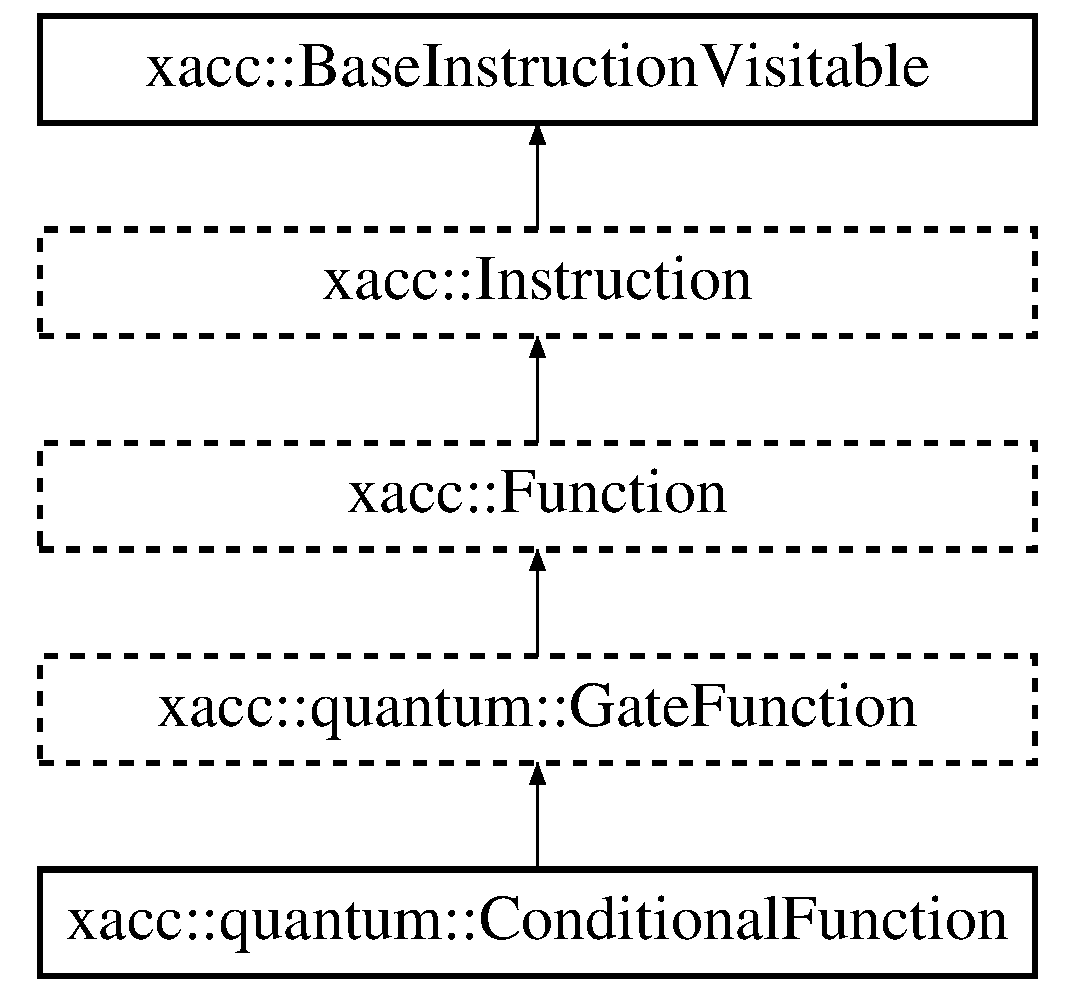
\includegraphics[height=7.887324cm]{a00021}
\end{center}
\end{figure}
\subsection*{Additional Inherited Members}


\subsection{Detailed Description}
F\+I\+X\+ME write this 

The documentation for this class was generated from the following file\+:\begin{DoxyCompactItemize}
\item 
All\+Gate\+Visitor.\+hpp\end{DoxyCompactItemize}

\hypertarget{a00022}{}\section{xacc\+:\+:quantum\+:\+:A\+Q\+C\+Accelerator\+Buffer Class Reference}
\label{a00022}\index{xacc\+::quantum\+::\+A\+Q\+C\+Accelerator\+Buffer@{xacc\+::quantum\+::\+A\+Q\+C\+Accelerator\+Buffer}}


{\ttfamily \#include $<$A\+Q\+C\+Accelerator\+Buffer.\+hpp$>$}

Inheritance diagram for xacc\+:\+:quantum\+:\+:A\+Q\+C\+Accelerator\+Buffer\+:\begin{figure}[H]
\begin{center}
\leavevmode
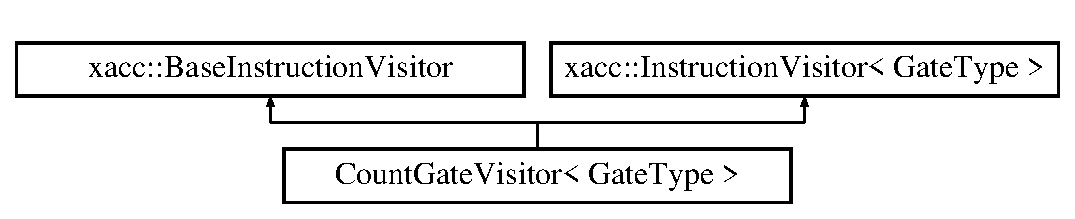
\includegraphics[height=2.000000cm]{a00022}
\end{center}
\end{figure}
\subsection*{Public Member Functions}
\begin{DoxyCompactItemize}
\item 
\hyperlink{a00022_ac2f9ea58140a27741b4dc8fceaa1ca5c}{A\+Q\+C\+Accelerator\+Buffer} (const std\+::string \&str, const int N)
\item 
{\footnotesize template$<$typename... Indices$>$ }\\\hyperlink{a00022_a628c742acf1d20fc8fe9b69f9be7b2c6}{A\+Q\+C\+Accelerator\+Buffer} (const std\+::string \&str, int first\+Index, Indices...\+indices)
\item 
void \hyperlink{a00022_a23992d11bdb6f093c0ce3f743677d4d9}{set\+Embedding} (std\+::map$<$ int, std\+::list$<$ int $>$$>$ emb)
\item 
std\+::map$<$ int, std\+::list$<$ int $>$ $>$ \hyperlink{a00022_ae98155c023d1b31b3b55a8c8e4ec6bc6}{get\+Embedding} ()
\end{DoxyCompactItemize}
\subsection*{Protected Attributes}
\begin{DoxyCompactItemize}
\item 
std\+::map$<$ int, std\+::list$<$ int $>$ $>$ \hyperlink{a00022_a26fd739244b0346cc3398eef31b11264}{embedding}
\item 
std\+::vector$<$ double $>$ \hyperlink{a00022_abe6d781724e197df449d8dfcde60e1a4}{energies}
\end{DoxyCompactItemize}


\subsection{Detailed Description}
The \hyperlink{a00022}{A\+Q\+C\+Accelerator\+Buffer} is an \hyperlink{a00019}{Accelerator\+Buffer} that keeps track of the problem-\/specific embedding into the hardware graph. It also tracks A\+QC Q\+PU computed energies. 

\subsection{Constructor \& Destructor Documentation}
\index{xacc\+::quantum\+::\+A\+Q\+C\+Accelerator\+Buffer@{xacc\+::quantum\+::\+A\+Q\+C\+Accelerator\+Buffer}!A\+Q\+C\+Accelerator\+Buffer@{A\+Q\+C\+Accelerator\+Buffer}}
\index{A\+Q\+C\+Accelerator\+Buffer@{A\+Q\+C\+Accelerator\+Buffer}!xacc\+::quantum\+::\+A\+Q\+C\+Accelerator\+Buffer@{xacc\+::quantum\+::\+A\+Q\+C\+Accelerator\+Buffer}}
\subsubsection[{\texorpdfstring{A\+Q\+C\+Accelerator\+Buffer(const std\+::string \&str, const int N)}{AQCAcceleratorBuffer(const std::string \&str, const int N)}}]{\setlength{\rightskip}{0pt plus 5cm}xacc\+::quantum\+::\+A\+Q\+C\+Accelerator\+Buffer\+::\+A\+Q\+C\+Accelerator\+Buffer (
\begin{DoxyParamCaption}
\item[{const std\+::string \&}]{str, }
\item[{const int}]{N}
\end{DoxyParamCaption}
)\hspace{0.3cm}{\ttfamily [inline]}}\hypertarget{a00022_ac2f9ea58140a27741b4dc8fceaa1ca5c}{}\label{a00022_ac2f9ea58140a27741b4dc8fceaa1ca5c}
The constructor 
\begin{DoxyParams}{Parameters}
{\em str} & The name of this buffer \\
\hline
{\em N} & The number of bits represented by this buffer \\
\hline
\end{DoxyParams}
\index{xacc\+::quantum\+::\+A\+Q\+C\+Accelerator\+Buffer@{xacc\+::quantum\+::\+A\+Q\+C\+Accelerator\+Buffer}!A\+Q\+C\+Accelerator\+Buffer@{A\+Q\+C\+Accelerator\+Buffer}}
\index{A\+Q\+C\+Accelerator\+Buffer@{A\+Q\+C\+Accelerator\+Buffer}!xacc\+::quantum\+::\+A\+Q\+C\+Accelerator\+Buffer@{xacc\+::quantum\+::\+A\+Q\+C\+Accelerator\+Buffer}}
\subsubsection[{\texorpdfstring{A\+Q\+C\+Accelerator\+Buffer(const std\+::string \&str, int first\+Index, Indices...\+indices)}{AQCAcceleratorBuffer(const std::string \&str, int firstIndex, Indices...indices)}}]{\setlength{\rightskip}{0pt plus 5cm}template$<$typename... Indices$>$ xacc\+::quantum\+::\+A\+Q\+C\+Accelerator\+Buffer\+::\+A\+Q\+C\+Accelerator\+Buffer (
\begin{DoxyParamCaption}
\item[{const std\+::string \&}]{str, }
\item[{int}]{first\+Index, }
\item[{Indices...}]{indices}
\end{DoxyParamCaption}
)\hspace{0.3cm}{\ttfamily [inline]}}\hypertarget{a00022_a628c742acf1d20fc8fe9b69f9be7b2c6}{}\label{a00022_a628c742acf1d20fc8fe9b69f9be7b2c6}
The constructor 
\begin{DoxyParams}{Parameters}
{\em str} & \\
\hline
{\em first\+Index} & \\
\hline
{\em indices} & \\
\hline
\end{DoxyParams}


\subsection{Member Function Documentation}
\index{xacc\+::quantum\+::\+A\+Q\+C\+Accelerator\+Buffer@{xacc\+::quantum\+::\+A\+Q\+C\+Accelerator\+Buffer}!get\+Embedding@{get\+Embedding}}
\index{get\+Embedding@{get\+Embedding}!xacc\+::quantum\+::\+A\+Q\+C\+Accelerator\+Buffer@{xacc\+::quantum\+::\+A\+Q\+C\+Accelerator\+Buffer}}
\subsubsection[{\texorpdfstring{get\+Embedding()}{getEmbedding()}}]{\setlength{\rightskip}{0pt plus 5cm}std\+::map$<$int, std\+::list$<$int$>$ $>$ xacc\+::quantum\+::\+A\+Q\+C\+Accelerator\+Buffer\+::get\+Embedding (
\begin{DoxyParamCaption}
{}
\end{DoxyParamCaption}
)\hspace{0.3cm}{\ttfamily [inline]}}\hypertarget{a00022_ae98155c023d1b31b3b55a8c8e4ec6bc6}{}\label{a00022_ae98155c023d1b31b3b55a8c8e4ec6bc6}
Return the minor graph embedding.

\begin{DoxyReturn}{Returns}
emb The minor graph embedding 
\end{DoxyReturn}
\index{xacc\+::quantum\+::\+A\+Q\+C\+Accelerator\+Buffer@{xacc\+::quantum\+::\+A\+Q\+C\+Accelerator\+Buffer}!set\+Embedding@{set\+Embedding}}
\index{set\+Embedding@{set\+Embedding}!xacc\+::quantum\+::\+A\+Q\+C\+Accelerator\+Buffer@{xacc\+::quantum\+::\+A\+Q\+C\+Accelerator\+Buffer}}
\subsubsection[{\texorpdfstring{set\+Embedding(std\+::map$<$ int, std\+::list$<$ int $>$$>$ emb)}{setEmbedding(std::map< int, std::list< int >> emb)}}]{\setlength{\rightskip}{0pt plus 5cm}void xacc\+::quantum\+::\+A\+Q\+C\+Accelerator\+Buffer\+::set\+Embedding (
\begin{DoxyParamCaption}
\item[{std\+::map$<$ int, std\+::list$<$ int $>$$>$}]{emb}
\end{DoxyParamCaption}
)\hspace{0.3cm}{\ttfamily [inline]}}\hypertarget{a00022_a23992d11bdb6f093c0ce3f743677d4d9}{}\label{a00022_a23992d11bdb6f093c0ce3f743677d4d9}
Set the minor graph embedding for the problem solved during this execution .


\begin{DoxyParams}{Parameters}
{\em emb} & The minor graph embedding \\
\hline
\end{DoxyParams}


\subsection{Member Data Documentation}
\index{xacc\+::quantum\+::\+A\+Q\+C\+Accelerator\+Buffer@{xacc\+::quantum\+::\+A\+Q\+C\+Accelerator\+Buffer}!embedding@{embedding}}
\index{embedding@{embedding}!xacc\+::quantum\+::\+A\+Q\+C\+Accelerator\+Buffer@{xacc\+::quantum\+::\+A\+Q\+C\+Accelerator\+Buffer}}
\subsubsection[{\texorpdfstring{embedding}{embedding}}]{\setlength{\rightskip}{0pt plus 5cm}std\+::map$<$int, std\+::list$<$int$>$ $>$ xacc\+::quantum\+::\+A\+Q\+C\+Accelerator\+Buffer\+::embedding\hspace{0.3cm}{\ttfamily [protected]}}\hypertarget{a00022_a26fd739244b0346cc3398eef31b11264}{}\label{a00022_a26fd739244b0346cc3398eef31b11264}
The minor graph embedding for the problem these results represent. \index{xacc\+::quantum\+::\+A\+Q\+C\+Accelerator\+Buffer@{xacc\+::quantum\+::\+A\+Q\+C\+Accelerator\+Buffer}!energies@{energies}}
\index{energies@{energies}!xacc\+::quantum\+::\+A\+Q\+C\+Accelerator\+Buffer@{xacc\+::quantum\+::\+A\+Q\+C\+Accelerator\+Buffer}}
\subsubsection[{\texorpdfstring{energies}{energies}}]{\setlength{\rightskip}{0pt plus 5cm}std\+::vector$<$double$>$ xacc\+::quantum\+::\+A\+Q\+C\+Accelerator\+Buffer\+::energies\hspace{0.3cm}{\ttfamily [protected]}}\hypertarget{a00022_abe6d781724e197df449d8dfcde60e1a4}{}\label{a00022_abe6d781724e197df449d8dfcde60e1a4}
The energies computed as part of this execution. 

The documentation for this class was generated from the following file\+:\begin{DoxyCompactItemize}
\item 
A\+Q\+C\+Accelerator\+Buffer.\+hpp\end{DoxyCompactItemize}

\hypertarget{a00023}{}\section{xacc\+:\+:Compiler Class Reference}
\label{a00023}\index{xacc\+::\+Compiler@{xacc\+::\+Compiler}}


{\ttfamily \#include $<$Compiler.\+hpp$>$}

Inheritance diagram for xacc\+:\+:Compiler\+:\begin{figure}[H]
\begin{center}
\leavevmode
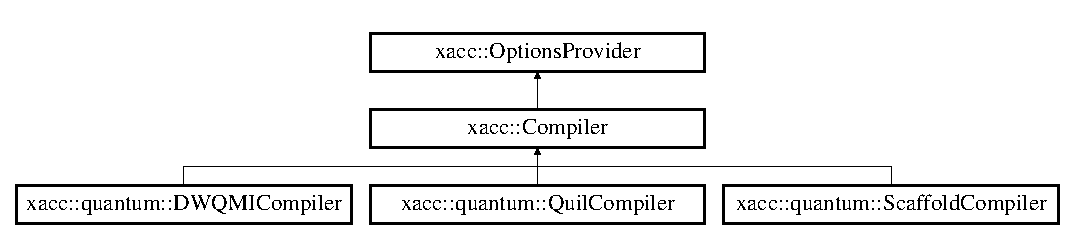
\includegraphics[height=2.772277cm]{a00023}
\end{center}
\end{figure}
\subsection*{Public Member Functions}
\begin{DoxyCompactItemize}
\item 
virtual std\+::shared\+\_\+ptr$<$ \hyperlink{a00051}{IR} $>$ \hyperlink{a00023_a546a40c95bb93af6a0c0ac48dbeaffc8}{compile} (const std\+::string \&src, std\+::shared\+\_\+ptr$<$ \hyperlink{a00011}{Accelerator} $>$ acc)=0
\item 
virtual std\+::shared\+\_\+ptr$<$ \hyperlink{a00051}{IR} $>$ \hyperlink{a00023_a9092f5f779b570c91569b59621280c04}{compile} (const std\+::string \&src)=0
\item 
virtual const std\+::string \hyperlink{a00023_aeedbe58a33fed29e4d7694ae743e25e7}{translate} (const std\+::string \&buffer\+Variable, std\+::shared\+\_\+ptr$<$ \hyperlink{a00039}{Function} $>$ function)=0
\item 
virtual const std\+::string \hyperlink{a00023_a87fca9100e6462122f5b687c3a0fb3fb}{get\+Name} ()=0
\item 
virtual std\+::shared\+\_\+ptr$<$ options\+\_\+description $>$ \hyperlink{a00023_a9f5a8965c9c2dd895016d18264ebbe92}{get\+Options} ()
\item 
virtual \hyperlink{a00023_a5d0b012687d9b44893872eaa81e47b38}{$\sim$\+Compiler} ()
\end{DoxyCompactItemize}
\subsection*{Protected Attributes}
\begin{DoxyCompactItemize}
\item 
std\+::string \hyperlink{a00023_a0ad81c816c09e5113d03cdc02165c453}{kernel\+Source}
\item 
std\+::shared\+\_\+ptr$<$ \hyperlink{a00011}{Accelerator} $>$ \hyperlink{a00023_ad4cbb467fa7e377bac6c054ffcb22b7c}{accelerator}
\end{DoxyCompactItemize}


\subsection{Detailed Description}
The \hyperlink{a00023}{Compiler} class provides an extensible interface for injecting custom compilation mechanisms into the X\+A\+CC framework. Implementations provide a compile method that takes the kernel source code string, performs compiler-\/specific compilation mechanism, and returns a valid X\+A\+CC \hyperlink{a00051}{IR} instance modeling the result of the compilation. 

\subsection{Constructor \& Destructor Documentation}
\index{xacc\+::\+Compiler@{xacc\+::\+Compiler}!````~Compiler@{$\sim$\+Compiler}}
\index{````~Compiler@{$\sim$\+Compiler}!xacc\+::\+Compiler@{xacc\+::\+Compiler}}
\subsubsection[{\texorpdfstring{$\sim$\+Compiler()}{~Compiler()}}]{\setlength{\rightskip}{0pt plus 5cm}virtual xacc\+::\+Compiler\+::$\sim$\+Compiler (
\begin{DoxyParamCaption}
{}
\end{DoxyParamCaption}
)\hspace{0.3cm}{\ttfamily [inline]}, {\ttfamily [virtual]}}\hypertarget{a00023_a5d0b012687d9b44893872eaa81e47b38}{}\label{a00023_a5d0b012687d9b44893872eaa81e47b38}
The destructor 

\subsection{Member Function Documentation}
\index{xacc\+::\+Compiler@{xacc\+::\+Compiler}!compile@{compile}}
\index{compile@{compile}!xacc\+::\+Compiler@{xacc\+::\+Compiler}}
\subsubsection[{\texorpdfstring{compile(const std\+::string \&src, std\+::shared\+\_\+ptr$<$ Accelerator $>$ acc)=0}{compile(const std::string \&src, std::shared\_ptr< Accelerator > acc)=0}}]{\setlength{\rightskip}{0pt plus 5cm}virtual std\+::shared\+\_\+ptr$<${\bf IR}$>$ xacc\+::\+Compiler\+::compile (
\begin{DoxyParamCaption}
\item[{const std\+::string \&}]{src, }
\item[{std\+::shared\+\_\+ptr$<$ {\bf Accelerator} $>$}]{acc}
\end{DoxyParamCaption}
)\hspace{0.3cm}{\ttfamily [pure virtual]}}\hypertarget{a00023_a546a40c95bb93af6a0c0ac48dbeaffc8}{}\label{a00023_a546a40c95bb93af6a0c0ac48dbeaffc8}
This method is to be implemented by derived Compilers and is in charge of executing the compilation mechanism on the provided source string. Implementations also are given access to the \hyperlink{a00011}{Accelerator} that this source code is intended for.


\begin{DoxyParams}{Parameters}
{\em src} & The kernel source string. \\
\hline
{\em acc} & The \hyperlink{a00011}{Accelerator} this code will be executed on \\
\hline
\end{DoxyParams}
\begin{DoxyReturn}{Returns}
ir Intermediate representation for provided source kernel code. 
\end{DoxyReturn}


Implemented in \hyperlink{a00034_a0df05642f1a6fd44ce7f1c0396d50c9c}{xacc\+::quantum\+::\+D\+W\+Q\+M\+I\+Compiler}, \hyperlink{a00078_a7caede75bb2304ba405966651b115543}{xacc\+::quantum\+::\+Scaffold\+Compiler}, and \hyperlink{a00063_a2421482415ca4e09963ea4ecddff8100}{xacc\+::quantum\+::\+Quil\+Compiler}.

\index{xacc\+::\+Compiler@{xacc\+::\+Compiler}!compile@{compile}}
\index{compile@{compile}!xacc\+::\+Compiler@{xacc\+::\+Compiler}}
\subsubsection[{\texorpdfstring{compile(const std\+::string \&src)=0}{compile(const std::string \&src)=0}}]{\setlength{\rightskip}{0pt plus 5cm}virtual std\+::shared\+\_\+ptr$<${\bf IR}$>$ xacc\+::\+Compiler\+::compile (
\begin{DoxyParamCaption}
\item[{const std\+::string \&}]{src}
\end{DoxyParamCaption}
)\hspace{0.3cm}{\ttfamily [pure virtual]}}\hypertarget{a00023_a9092f5f779b570c91569b59621280c04}{}\label{a00023_a9092f5f779b570c91569b59621280c04}
This method is to be implemented by derived Compilers and is in charge of executing the compilation mechanism on the provided source string. 
\begin{DoxyParams}{Parameters}
{\em src} & \\
\hline
\end{DoxyParams}
\begin{DoxyReturn}{Returns}

\end{DoxyReturn}


Implemented in \hyperlink{a00034_aa22591343b5509bf2c3a5820130ba906}{xacc\+::quantum\+::\+D\+W\+Q\+M\+I\+Compiler}, \hyperlink{a00078_a3736ecc229fe6acdd4c991e85d7a1f08}{xacc\+::quantum\+::\+Scaffold\+Compiler}, and \hyperlink{a00063_adf4d321ecb0df3fa7728999f941c83b2}{xacc\+::quantum\+::\+Quil\+Compiler}.

\index{xacc\+::\+Compiler@{xacc\+::\+Compiler}!get\+Name@{get\+Name}}
\index{get\+Name@{get\+Name}!xacc\+::\+Compiler@{xacc\+::\+Compiler}}
\subsubsection[{\texorpdfstring{get\+Name()=0}{getName()=0}}]{\setlength{\rightskip}{0pt plus 5cm}virtual const std\+::string xacc\+::\+Compiler\+::get\+Name (
\begin{DoxyParamCaption}
{}
\end{DoxyParamCaption}
)\hspace{0.3cm}{\ttfamily [pure virtual]}}\hypertarget{a00023_a87fca9100e6462122f5b687c3a0fb3fb}{}\label{a00023_a87fca9100e6462122f5b687c3a0fb3fb}
Return the name of this \hyperlink{a00023}{Compiler} \begin{DoxyReturn}{Returns}
name \hyperlink{a00023}{Compiler} name 
\end{DoxyReturn}


Implemented in \hyperlink{a00034_aed42de96f8e0dd94b6de183f28aee419}{xacc\+::quantum\+::\+D\+W\+Q\+M\+I\+Compiler}, \hyperlink{a00078_a3f537054a3924a1d14f4ceb0f0181161}{xacc\+::quantum\+::\+Scaffold\+Compiler}, and \hyperlink{a00063_ae7d52140b6dd52730edc6e38ae48f437}{xacc\+::quantum\+::\+Quil\+Compiler}.

\index{xacc\+::\+Compiler@{xacc\+::\+Compiler}!get\+Options@{get\+Options}}
\index{get\+Options@{get\+Options}!xacc\+::\+Compiler@{xacc\+::\+Compiler}}
\subsubsection[{\texorpdfstring{get\+Options()}{getOptions()}}]{\setlength{\rightskip}{0pt plus 5cm}virtual std\+::shared\+\_\+ptr$<$options\+\_\+description$>$ xacc\+::\+Compiler\+::get\+Options (
\begin{DoxyParamCaption}
{}
\end{DoxyParamCaption}
)\hspace{0.3cm}{\ttfamily [inline]}, {\ttfamily [virtual]}}\hypertarget{a00023_a9f5a8965c9c2dd895016d18264ebbe92}{}\label{a00023_a9f5a8965c9c2dd895016d18264ebbe92}
Return an empty options\+\_\+description, this is for subclasses to implement. 

Implements \hyperlink{a00057_a6d150954f852109bfe2c1ae90222926f}{xacc\+::\+Options\+Provider}.



Reimplemented in \hyperlink{a00034_a0851334cc33b5b1da2694150a0a1a43c}{xacc\+::quantum\+::\+D\+W\+Q\+M\+I\+Compiler}.

\index{xacc\+::\+Compiler@{xacc\+::\+Compiler}!translate@{translate}}
\index{translate@{translate}!xacc\+::\+Compiler@{xacc\+::\+Compiler}}
\subsubsection[{\texorpdfstring{translate(const std\+::string \&buffer\+Variable, std\+::shared\+\_\+ptr$<$ Function $>$ function)=0}{translate(const std::string \&bufferVariable, std::shared\_ptr< Function > function)=0}}]{\setlength{\rightskip}{0pt plus 5cm}virtual const std\+::string xacc\+::\+Compiler\+::translate (
\begin{DoxyParamCaption}
\item[{const std\+::string \&}]{buffer\+Variable, }
\item[{std\+::shared\+\_\+ptr$<$ {\bf Function} $>$}]{function}
\end{DoxyParamCaption}
)\hspace{0.3cm}{\ttfamily [pure virtual]}}\hypertarget{a00023_aeedbe58a33fed29e4d7694ae743e25e7}{}\label{a00023_aeedbe58a33fed29e4d7694ae743e25e7}
This method is to be implemented by derived Compilers and is in charge of taking the provided \hyperlink{a00039}{Function} \hyperlink{a00051}{IR} and converting it to source code in this \hyperlink{a00023}{Compiler}\textquotesingle{}s language.


\begin{DoxyParams}{Parameters}
{\em function} & The X\+A\+CC \hyperlink{a00051}{IR} \hyperlink{a00039}{Function} to translate \\
\hline
\end{DoxyParams}
\begin{DoxyReturn}{Returns}
src The source code as a string 
\end{DoxyReturn}


Implemented in \hyperlink{a00034_a56a345539665099329209b3b5f6810c9}{xacc\+::quantum\+::\+D\+W\+Q\+M\+I\+Compiler}, \hyperlink{a00063_a66ca00bbb1f30e7bc6dd86b1e267b93b}{xacc\+::quantum\+::\+Quil\+Compiler}, and \hyperlink{a00078_ac7ca2941e987ba579c6f50cfbd7fb0dc}{xacc\+::quantum\+::\+Scaffold\+Compiler}.



\subsection{Member Data Documentation}
\index{xacc\+::\+Compiler@{xacc\+::\+Compiler}!accelerator@{accelerator}}
\index{accelerator@{accelerator}!xacc\+::\+Compiler@{xacc\+::\+Compiler}}
\subsubsection[{\texorpdfstring{accelerator}{accelerator}}]{\setlength{\rightskip}{0pt plus 5cm}std\+::shared\+\_\+ptr$<${\bf Accelerator}$>$ xacc\+::\+Compiler\+::accelerator\hspace{0.3cm}{\ttfamily [protected]}}\hypertarget{a00023_ad4cbb467fa7e377bac6c054ffcb22b7c}{}\label{a00023_ad4cbb467fa7e377bac6c054ffcb22b7c}
Reference to the \hyperlink{a00011}{Accelerator} that this compiler is targeting. \index{xacc\+::\+Compiler@{xacc\+::\+Compiler}!kernel\+Source@{kernel\+Source}}
\index{kernel\+Source@{kernel\+Source}!xacc\+::\+Compiler@{xacc\+::\+Compiler}}
\subsubsection[{\texorpdfstring{kernel\+Source}{kernelSource}}]{\setlength{\rightskip}{0pt plus 5cm}std\+::string xacc\+::\+Compiler\+::kernel\+Source\hspace{0.3cm}{\ttfamily [protected]}}\hypertarget{a00023_a0ad81c816c09e5113d03cdc02165c453}{}\label{a00023_a0ad81c816c09e5113d03cdc02165c453}
Reference to the provided kernel source code string 

The documentation for this class was generated from the following file\+:\begin{DoxyCompactItemize}
\item 
Compiler.\+hpp\end{DoxyCompactItemize}

\hypertarget{a00024}{}\section{xacc\+:\+:Base\+Instruction\+Visitor Class Reference}
\label{a00024}\index{xacc\+::\+Base\+Instruction\+Visitor@{xacc\+::\+Base\+Instruction\+Visitor}}


{\ttfamily \#include $<$Instruction\+Visitor.\+hpp$>$}

Inheritance diagram for xacc\+:\+:Base\+Instruction\+Visitor\+:\begin{figure}[H]
\begin{center}
\leavevmode
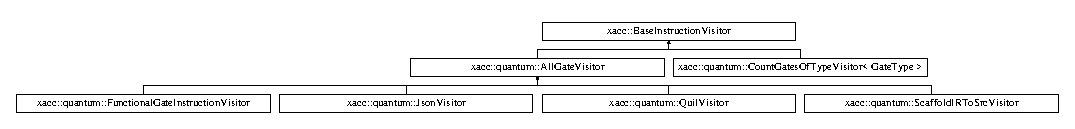
\includegraphics[height=1.288344cm]{a00024}
\end{center}
\end{figure}
\subsection*{Public Member Functions}
\begin{DoxyCompactItemize}
\item 
virtual \hyperlink{a00024_aa6f5104f5868fe1eca9be4dc4036eba4}{$\sim$\+Base\+Instruction\+Visitor} ()
\end{DoxyCompactItemize}


\subsection{Detailed Description}
The \hyperlink{a00024}{Base\+Instruction\+Visitor} is a base class for all classes that are \hyperlink{a00072}{Instruction} visitors. It basically provides a means for passing instruction visitor handles in a polymorphic manner. 

\subsection{Constructor \& Destructor Documentation}
\index{xacc\+::\+Base\+Instruction\+Visitor@{xacc\+::\+Base\+Instruction\+Visitor}!````~Base\+Instruction\+Visitor@{$\sim$\+Base\+Instruction\+Visitor}}
\index{````~Base\+Instruction\+Visitor@{$\sim$\+Base\+Instruction\+Visitor}!xacc\+::\+Base\+Instruction\+Visitor@{xacc\+::\+Base\+Instruction\+Visitor}}
\subsubsection[{\texorpdfstring{$\sim$\+Base\+Instruction\+Visitor()}{~BaseInstructionVisitor()}}]{\setlength{\rightskip}{0pt plus 5cm}virtual xacc\+::\+Base\+Instruction\+Visitor\+::$\sim$\+Base\+Instruction\+Visitor (
\begin{DoxyParamCaption}
{}
\end{DoxyParamCaption}
)\hspace{0.3cm}{\ttfamily [inline]}, {\ttfamily [virtual]}}\hypertarget{a00024_aa6f5104f5868fe1eca9be4dc4036eba4}{}\label{a00024_aa6f5104f5868fe1eca9be4dc4036eba4}
The destructor 

The documentation for this class was generated from the following file\+:\begin{DoxyCompactItemize}
\item 
Instruction\+Visitor.\+hpp\end{DoxyCompactItemize}

\hypertarget{a00025}{}\section{xacc\+:\+:quantum\+:\+:Conditional\+Function Class Reference}
\label{a00025}\index{xacc\+::quantum\+::\+Conditional\+Function@{xacc\+::quantum\+::\+Conditional\+Function}}
Inheritance diagram for xacc\+:\+:quantum\+:\+:Conditional\+Function\+:\begin{figure}[H]
\begin{center}
\leavevmode
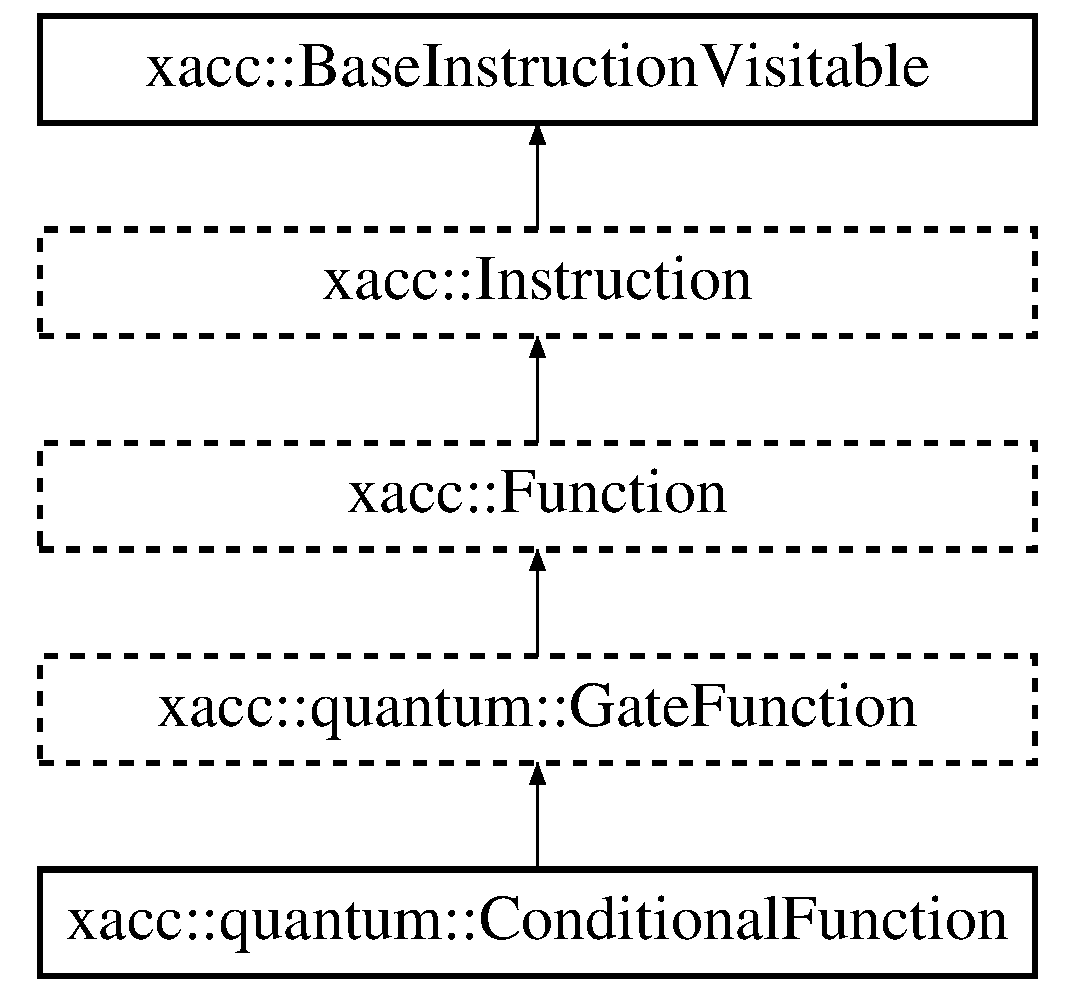
\includegraphics[height=5.000000cm]{a00025}
\end{center}
\end{figure}
\subsection*{Public Member Functions}
\begin{DoxyCompactItemize}
\item 
{\bfseries Conditional\+Function} (int qbit)\hypertarget{a00025_aa28610a08ae04d62ccdd8359433100c3}{}\label{a00025_aa28610a08ae04d62ccdd8359433100c3}

\item 
virtual void \hyperlink{a00025_a6aedad20f96390880efdc0a476b3273f}{add\+Instruction} (Inst\+Ptr instruction)
\item 
const int {\bfseries get\+Conditional\+Qubit} ()\hypertarget{a00025_a804317333b6677a041a3071b5108c0df}{}\label{a00025_a804317333b6677a041a3071b5108c0df}

\item 
void {\bfseries evaluate} (const int acc\+Bit\+State)\hypertarget{a00025_a709c236a5beb62d9a3bd5265196fb6c9}{}\label{a00025_a709c236a5beb62d9a3bd5265196fb6c9}

\item 
virtual const std\+::string \hyperlink{a00025_aca7a5f849fece6fc28a904efee9a3370}{to\+String} (const std\+::string \&buffer\+Var\+Name)
\end{DoxyCompactItemize}
\subsection*{Protected Attributes}
\begin{DoxyCompactItemize}
\item 
int {\bfseries qbit\+Idx}\hypertarget{a00025_a0310536801417c0eded28a4dea1efa44}{}\label{a00025_a0310536801417c0eded28a4dea1efa44}

\end{DoxyCompactItemize}
\subsection*{Additional Inherited Members}


\subsection{Member Function Documentation}
\index{xacc\+::quantum\+::\+Conditional\+Function@{xacc\+::quantum\+::\+Conditional\+Function}!add\+Instruction@{add\+Instruction}}
\index{add\+Instruction@{add\+Instruction}!xacc\+::quantum\+::\+Conditional\+Function@{xacc\+::quantum\+::\+Conditional\+Function}}
\subsubsection[{\texorpdfstring{add\+Instruction(\+Inst\+Ptr instruction)}{addInstruction(InstPtr instruction)}}]{\setlength{\rightskip}{0pt plus 5cm}void xacc\+::quantum\+::\+Conditional\+Function\+::add\+Instruction (
\begin{DoxyParamCaption}
\item[{Inst\+Ptr}]{instruction}
\end{DoxyParamCaption}
)\hspace{0.3cm}{\ttfamily [virtual]}}\hypertarget{a00025_a6aedad20f96390880efdc0a476b3273f}{}\label{a00025_a6aedad20f96390880efdc0a476b3273f}
Add an instruction to this quantum intermediate representation.


\begin{DoxyParams}{Parameters}
{\em instruction} & \\
\hline
\end{DoxyParams}


Reimplemented from \hyperlink{a00040_a892fb69a10f0a7cb5abdab4cca61b80a}{xacc\+::quantum\+::\+Gate\+Function}.

\index{xacc\+::quantum\+::\+Conditional\+Function@{xacc\+::quantum\+::\+Conditional\+Function}!to\+String@{to\+String}}
\index{to\+String@{to\+String}!xacc\+::quantum\+::\+Conditional\+Function@{xacc\+::quantum\+::\+Conditional\+Function}}
\subsubsection[{\texorpdfstring{to\+String(const std\+::string \&buffer\+Var\+Name)}{toString(const std::string \&bufferVarName)}}]{\setlength{\rightskip}{0pt plus 5cm}const std\+::string xacc\+::quantum\+::\+Conditional\+Function\+::to\+String (
\begin{DoxyParamCaption}
\item[{const std\+::string \&}]{buffer\+Var\+Name}
\end{DoxyParamCaption}
)\hspace{0.3cm}{\ttfamily [virtual]}}\hypertarget{a00025_aca7a5f849fece6fc28a904efee9a3370}{}\label{a00025_aca7a5f849fece6fc28a904efee9a3370}
Return an assembly-\/like string representation for this function . 
\begin{DoxyParams}{Parameters}
{\em buffer\+Var\+Name} & \\
\hline
\end{DoxyParams}
\begin{DoxyReturn}{Returns}

\end{DoxyReturn}


Reimplemented from \hyperlink{a00040_aa1950776ae84bad2d0795a0441f910e7}{xacc\+::quantum\+::\+Gate\+Function}.



The documentation for this class was generated from the following files\+:\begin{DoxyCompactItemize}
\item 
Conditional\+Function.\+hpp\item 
Conditional\+Function.\+cpp\end{DoxyCompactItemize}

\hypertarget{a00026}{}\section{xacc\+:\+:quantum\+:\+:D\+Wave\+Vertex Class Reference}
\label{a00026}\index{xacc\+::quantum\+::\+D\+Wave\+Vertex@{xacc\+::quantum\+::\+D\+Wave\+Vertex}}


{\ttfamily \#include $<$Embedding\+Algorithm.\+hpp$>$}

Inheritance diagram for xacc\+:\+:quantum\+:\+:D\+Wave\+Vertex\+:\begin{figure}[H]
\begin{center}
\leavevmode
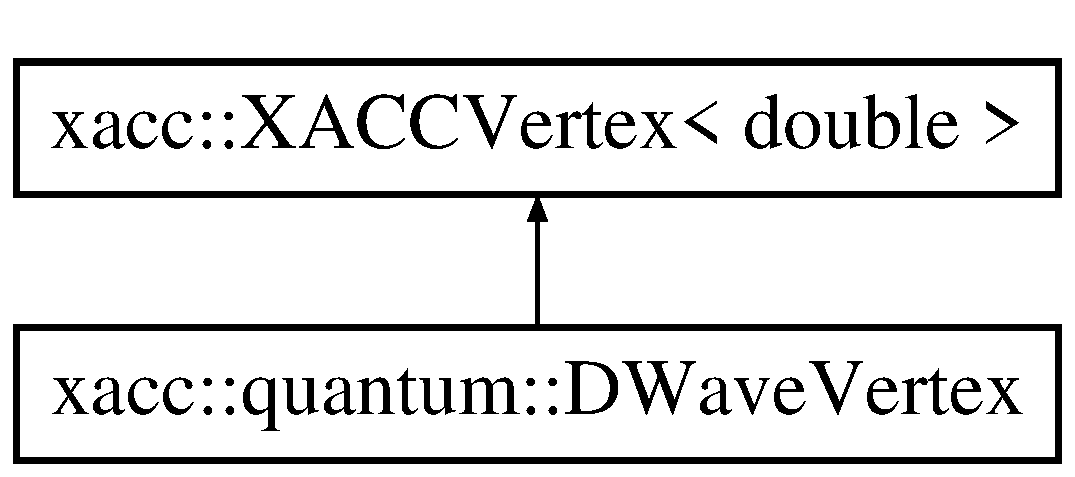
\includegraphics[height=2.000000cm]{a00026}
\end{center}
\end{figure}
\subsection*{Additional Inherited Members}


\subsection{Detailed Description}
The \hyperlink{a00026}{D\+Wave\+Vertex} is a subclass of the \hyperlink{a00073}{X\+A\+C\+C\+Vertex} that keeps track of one vertex parameter -\/ the qubit bias parameter. \hyperlink{a00073}{X\+A\+C\+C\+Vertex} already keeps track of edge weights. 

The documentation for this class was generated from the following file\+:\begin{DoxyCompactItemize}
\item 
Embedding\+Algorithm.\+hpp\end{DoxyCompactItemize}

\hypertarget{a00027}{}\section{xacc\+:\+:quantum\+:\+:Embedding\+Algorithm Class Reference}
\label{a00027}\index{xacc\+::quantum\+::\+Embedding\+Algorithm@{xacc\+::quantum\+::\+Embedding\+Algorithm}}


{\ttfamily \#include $<$Embedding\+Algorithm.\+hpp$>$}

\subsection*{Public Member Functions}
\begin{DoxyCompactItemize}
\item 
\hyperlink{a00027_abad06507eef6b63af0884e3a96145c69}{Embedding\+Algorithm} ()
\item 
virtual \hyperlink{a00027_aa43660ad5d4c4b3ac67863892c33dc51}{$\sim$\+Embedding\+Algorithm} ()
\item 
virtual std\+::map$<$ int, std\+::list$<$ int $>$ $>$ \hyperlink{a00027_a67158c0f4925ff6b85698efec61e1175}{embed} (std\+::shared\+\_\+ptr$<$ \hyperlink{a00035}{D\+Wave\+Graph} $>$ problem, std\+::shared\+\_\+ptr$<$ \hyperlink{a00035}{D\+Wave\+Graph} $>$ hardware, std\+::map$<$ std\+::string, std\+::string $>$ params=std\+::map$<$ std\+::string, std\+::string $>$())=0
\item 
virtual std\+::string \hyperlink{a00027_a21079dc8ee37792977f5fd209e3f3b19}{name} ()=0
\end{DoxyCompactItemize}


\subsection{Detailed Description}
The \hyperlink{a00027}{Embedding\+Algorithm} class provides an interface for minor graph embedding algorithms. 

\subsection{Constructor \& Destructor Documentation}
\index{xacc\+::quantum\+::\+Embedding\+Algorithm@{xacc\+::quantum\+::\+Embedding\+Algorithm}!Embedding\+Algorithm@{Embedding\+Algorithm}}
\index{Embedding\+Algorithm@{Embedding\+Algorithm}!xacc\+::quantum\+::\+Embedding\+Algorithm@{xacc\+::quantum\+::\+Embedding\+Algorithm}}
\subsubsection[{\texorpdfstring{Embedding\+Algorithm()}{EmbeddingAlgorithm()}}]{\setlength{\rightskip}{0pt plus 5cm}xacc\+::quantum\+::\+Embedding\+Algorithm\+::\+Embedding\+Algorithm (
\begin{DoxyParamCaption}
{}
\end{DoxyParamCaption}
)\hspace{0.3cm}{\ttfamily [inline]}}\hypertarget{a00027_abad06507eef6b63af0884e3a96145c69}{}\label{a00027_abad06507eef6b63af0884e3a96145c69}
The Constructor \index{xacc\+::quantum\+::\+Embedding\+Algorithm@{xacc\+::quantum\+::\+Embedding\+Algorithm}!````~Embedding\+Algorithm@{$\sim$\+Embedding\+Algorithm}}
\index{````~Embedding\+Algorithm@{$\sim$\+Embedding\+Algorithm}!xacc\+::quantum\+::\+Embedding\+Algorithm@{xacc\+::quantum\+::\+Embedding\+Algorithm}}
\subsubsection[{\texorpdfstring{$\sim$\+Embedding\+Algorithm()}{~EmbeddingAlgorithm()}}]{\setlength{\rightskip}{0pt plus 5cm}virtual xacc\+::quantum\+::\+Embedding\+Algorithm\+::$\sim$\+Embedding\+Algorithm (
\begin{DoxyParamCaption}
{}
\end{DoxyParamCaption}
)\hspace{0.3cm}{\ttfamily [inline]}, {\ttfamily [virtual]}}\hypertarget{a00027_aa43660ad5d4c4b3ac67863892c33dc51}{}\label{a00027_aa43660ad5d4c4b3ac67863892c33dc51}
The Destructor 

\subsection{Member Function Documentation}
\index{xacc\+::quantum\+::\+Embedding\+Algorithm@{xacc\+::quantum\+::\+Embedding\+Algorithm}!embed@{embed}}
\index{embed@{embed}!xacc\+::quantum\+::\+Embedding\+Algorithm@{xacc\+::quantum\+::\+Embedding\+Algorithm}}
\subsubsection[{\texorpdfstring{embed(std\+::shared\+\_\+ptr$<$ D\+Wave\+Graph $>$ problem, std\+::shared\+\_\+ptr$<$ D\+Wave\+Graph $>$ hardware, std\+::map$<$ std\+::string, std\+::string $>$ params=std\+::map$<$ std\+::string, std\+::string $>$())=0}{embed(std::shared\_ptr< DWaveGraph > problem, std::shared\_ptr< DWaveGraph > hardware, std::map< std::string, std::string > params=std::map< std::string, std::string >())=0}}]{\setlength{\rightskip}{0pt plus 5cm}virtual std\+::map$<$int, std\+::list$<$int$>$ $>$ xacc\+::quantum\+::\+Embedding\+Algorithm\+::embed (
\begin{DoxyParamCaption}
\item[{std\+::shared\+\_\+ptr$<$ {\bf D\+Wave\+Graph} $>$}]{problem, }
\item[{std\+::shared\+\_\+ptr$<$ {\bf D\+Wave\+Graph} $>$}]{hardware, }
\item[{std\+::map$<$ std\+::string, std\+::string $>$}]{params = {\ttfamily std\+:\+:map$<$~std\+:\+:string,~std\+:\+:string~$>$()}}
\end{DoxyParamCaption}
)\hspace{0.3cm}{\ttfamily [pure virtual]}}\hypertarget{a00027_a67158c0f4925ff6b85698efec61e1175}{}\label{a00027_a67158c0f4925ff6b85698efec61e1175}
Implementations of \hyperlink{a00027}{Embedding\+Algorithm} implement this method to provide a valid minor graph embedding of the given problem graph into the given hardware graph.


\begin{DoxyParams}{Parameters}
{\em problem} & The problem graph to be embedded into the hardware graph \\
\hline
{\em hardware} & The hardware graph. \\
\hline
{\em params} & Any key-\/value string parameters to influence the algorithm. \\
\hline
\end{DoxyParams}
\begin{DoxyReturn}{Returns}
embedding A mapping of problem vertex indices to the list of hardware vertices they map to 
\end{DoxyReturn}
\index{xacc\+::quantum\+::\+Embedding\+Algorithm@{xacc\+::quantum\+::\+Embedding\+Algorithm}!name@{name}}
\index{name@{name}!xacc\+::quantum\+::\+Embedding\+Algorithm@{xacc\+::quantum\+::\+Embedding\+Algorithm}}
\subsubsection[{\texorpdfstring{name()=0}{name()=0}}]{\setlength{\rightskip}{0pt plus 5cm}virtual std\+::string xacc\+::quantum\+::\+Embedding\+Algorithm\+::name (
\begin{DoxyParamCaption}
{}
\end{DoxyParamCaption}
)\hspace{0.3cm}{\ttfamily [pure virtual]}}\hypertarget{a00027_a21079dc8ee37792977f5fd209e3f3b19}{}\label{a00027_a21079dc8ee37792977f5fd209e3f3b19}
Return the name of this Embedding Algorithm \begin{DoxyReturn}{Returns}

\end{DoxyReturn}


The documentation for this class was generated from the following file\+:\begin{DoxyCompactItemize}
\item 
Embedding\+Algorithm.\+hpp\end{DoxyCompactItemize}

\hypertarget{a00028}{}\section{xacc\+:\+:quantum\+:\+:Chimera\+Graph Class Reference}
\label{a00028}\index{xacc\+::quantum\+::\+Chimera\+Graph@{xacc\+::quantum\+::\+Chimera\+Graph}}
Inheritance diagram for xacc\+:\+:quantum\+:\+:Chimera\+Graph\+:\begin{figure}[H]
\begin{center}
\leavevmode
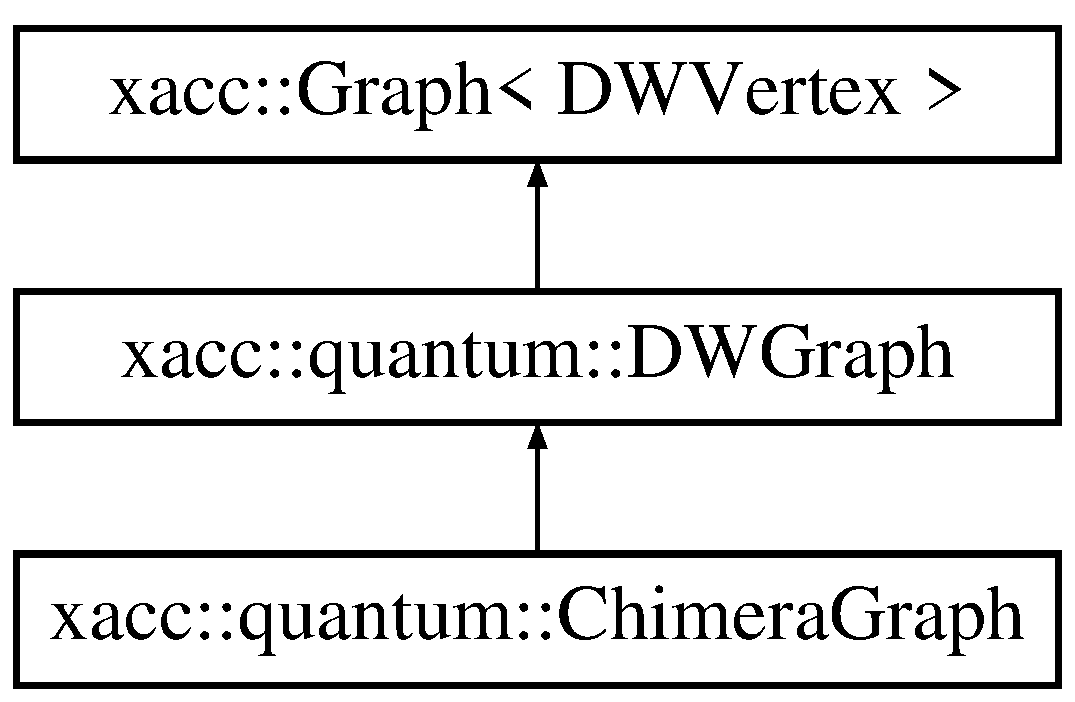
\includegraphics[height=3.000000cm]{a00028}
\end{center}
\end{figure}
\subsection*{Public Member Functions}
\begin{DoxyCompactItemize}
\item 
{\bfseries Chimera\+Graph} (int grid\+Size)\hypertarget{a00028_a64f23e464ba85d6625fe1fc2d2608052}{}\label{a00028_a64f23e464ba85d6625fe1fc2d2608052}

\end{DoxyCompactItemize}
\subsection*{Additional Inherited Members}


The documentation for this class was generated from the following file\+:\begin{DoxyCompactItemize}
\item 
D\+W\+Graph.\+hpp\end{DoxyCompactItemize}

\hypertarget{a00029}{}\section{Fake\+Http\+Client Class Reference}
\label{a00029}\index{Fake\+Http\+Client@{Fake\+Http\+Client}}
Inheritance diagram for Fake\+Http\+Client\+:\begin{figure}[H]
\begin{center}
\leavevmode
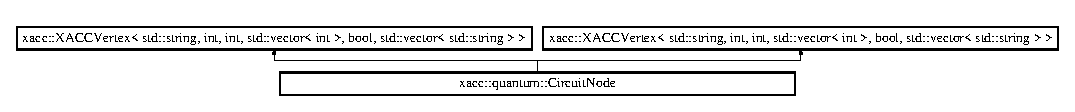
\includegraphics[height=2.000000cm]{a00029}
\end{center}
\end{figure}
\subsection*{Public Member Functions}
\begin{DoxyCompactItemize}
\item 
virtual fire\+::util\+::\+Http\+Response {\bfseries get} (const std\+::string \&relative\+Path, const std\+::map$<$ std\+::string, std\+::string $>$ \&header=std\+::map$<$ std\+::string, std\+::string $>$())\hypertarget{a00029_aa69081dbfa2351dbc9d01434df577568}{}\label{a00029_aa69081dbfa2351dbc9d01434df577568}

\item 
virtual fire\+::util\+::\+Http\+Response \hyperlink{a00029_af775ada9f2a4e0939f06b733acb5e8ed}{post} (const std\+::string \&relative\+Path, const std\+::string \&message, const std\+::map$<$ std\+::string, std\+::string $>$ \&header=std\+::map$<$ std\+::string, std\+::string $>$())
\end{DoxyCompactItemize}
\subsection*{Public Attributes}
\begin{DoxyCompactItemize}
\item 
bool {\bfseries post\+Occured} = false\hypertarget{a00029_aa4f56c4906c5c5654f05778b97860441}{}\label{a00029_aa4f56c4906c5c5654f05778b97860441}

\end{DoxyCompactItemize}


\subsection{Member Function Documentation}
\index{Fake\+Http\+Client@{Fake\+Http\+Client}!post@{post}}
\index{post@{post}!Fake\+Http\+Client@{Fake\+Http\+Client}}
\subsubsection[{\texorpdfstring{post(const std\+::string \&relative\+Path, const std\+::string \&message, const std\+::map$<$ std\+::string, std\+::string $>$ \&header=std\+::map$<$ std\+::string, std\+::string $>$())}{post(const std::string \&relativePath, const std::string \&message, const std::map< std::string, std::string > \&header=std::map< std::string, std::string >())}}]{\setlength{\rightskip}{0pt plus 5cm}virtual fire\+::util\+::\+Http\+Response Fake\+Http\+Client\+::post (
\begin{DoxyParamCaption}
\item[{const std\+::string \&}]{relative\+Path, }
\item[{const std\+::string \&}]{message, }
\item[{const std\+::map$<$ std\+::string, std\+::string $>$ \&}]{header = {\ttfamily std\+:\+:map$<$~std\+:\+:string,~std\+:\+:string$>$()}}
\end{DoxyParamCaption}
)\hspace{0.3cm}{\ttfamily [inline]}, {\ttfamily [virtual]}}\hypertarget{a00029_af775ada9f2a4e0939f06b733acb5e8ed}{}\label{a00029_af775ada9f2a4e0939f06b733acb5e8ed}
Issue an H\+T\+TP Post command at the given relative path with the provided message. Clients can provide a map of header key values to modify the P\+O\+ST request.


\begin{DoxyParams}{Parameters}
{\em relative\+Path} & The path relative to the hostname/port provided to this Networking\+Tool \\
\hline
{\em message} & The message to post \\
\hline
{\em header} & The map of additional H\+T\+TP P\+O\+ST header information \\
\hline
\end{DoxyParams}
\begin{DoxyReturn}{Returns}
success Boolean indicating if post was successful 
\end{DoxyReturn}


The documentation for this class was generated from the following file\+:\begin{DoxyCompactItemize}
\item 
Rigetti\+Accelerator\+Tester.\+cpp\end{DoxyCompactItemize}

\hypertarget{a00030}{}\section{xacc\+:\+:C\+L\+I\+Parser Class Reference}
\label{a00030}\index{xacc\+::\+C\+L\+I\+Parser@{xacc\+::\+C\+L\+I\+Parser}}


{\ttfamily \#include $<$C\+L\+I\+Parser.\+hpp$>$}

\subsection*{Public Member Functions}
\begin{DoxyCompactItemize}
\item 
\hyperlink{a00030_a041f8ba22cf5e1dd1fdcdc6c9223b405}{C\+L\+I\+Parser} ()
\item 
void \hyperlink{a00030_ae6499c8c7da9b4f453757dd86028a14f}{parse} (int argc, char $\ast$$\ast$argv)
\item 
void {\bfseries add\+String\+Option} (const std\+::string key, const std\+::string description=\char`\"{}\char`\"{})\hypertarget{a00030_a793192114817fb3a9221232eab0307fd}{}\label{a00030_a793192114817fb3a9221232eab0307fd}

\end{DoxyCompactItemize}
\subsection*{Protected Attributes}
\begin{DoxyCompactItemize}
\item 
std\+::shared\+\_\+ptr$<$ options\+\_\+description $>$ \hyperlink{a00030_a0f1564966cc40c340027aecb386c4469}{xacc\+Options}
\end{DoxyCompactItemize}


\subsection{Detailed Description}
The role of the \hyperlink{a00030}{C\+L\+I\+Parser} is to parse all command line options provided to an X\+A\+C\+C-\/enabled program. It takes upon construction to available argc and argv variables from the command line, and parses them to fill the \hyperlink{a00113}{Runtime\+Options} singleton and load any X\+A\+CC \hyperlink{a00034}{Compiler} or \hyperlink{a00017}{Accelerator} plugins.

It also queries all available Option\+Providers to display all available options to the X\+A\+CC user. 

\subsection{Constructor \& Destructor Documentation}
\index{xacc\+::\+C\+L\+I\+Parser@{xacc\+::\+C\+L\+I\+Parser}!C\+L\+I\+Parser@{C\+L\+I\+Parser}}
\index{C\+L\+I\+Parser@{C\+L\+I\+Parser}!xacc\+::\+C\+L\+I\+Parser@{xacc\+::\+C\+L\+I\+Parser}}
\subsubsection[{\texorpdfstring{C\+L\+I\+Parser()}{CLIParser()}}]{\setlength{\rightskip}{0pt plus 5cm}xacc\+::\+C\+L\+I\+Parser\+::\+C\+L\+I\+Parser (
\begin{DoxyParamCaption}
{}
\end{DoxyParamCaption}
)\hspace{0.3cm}{\ttfamily [inline]}}\hypertarget{a00030_a041f8ba22cf5e1dd1fdcdc6c9223b405}{}\label{a00030_a041f8ba22cf5e1dd1fdcdc6c9223b405}
The constructor 

\subsection{Member Function Documentation}
\index{xacc\+::\+C\+L\+I\+Parser@{xacc\+::\+C\+L\+I\+Parser}!parse@{parse}}
\index{parse@{parse}!xacc\+::\+C\+L\+I\+Parser@{xacc\+::\+C\+L\+I\+Parser}}
\subsubsection[{\texorpdfstring{parse(int argc, char $\ast$$\ast$argv)}{parse(int argc, char **argv)}}]{\setlength{\rightskip}{0pt plus 5cm}void xacc\+::\+C\+L\+I\+Parser\+::parse (
\begin{DoxyParamCaption}
\item[{int}]{argc, }
\item[{char $\ast$$\ast$}]{argv}
\end{DoxyParamCaption}
)\hspace{0.3cm}{\ttfamily [inline]}}\hypertarget{a00030_ae6499c8c7da9b4f453757dd86028a14f}{}\label{a00030_ae6499c8c7da9b4f453757dd86028a14f}
Parse the command line options. Provide a Boost options\+\_\+description built up and provided by all available Options\+Providers. This method also loads all Compilers and Accelerators available in the X\+A\+C\+C\+\_\+\+I\+N\+S\+T\+A\+L\+L\+\_\+\+D\+IR. 

\subsection{Member Data Documentation}
\index{xacc\+::\+C\+L\+I\+Parser@{xacc\+::\+C\+L\+I\+Parser}!xacc\+Options@{xacc\+Options}}
\index{xacc\+Options@{xacc\+Options}!xacc\+::\+C\+L\+I\+Parser@{xacc\+::\+C\+L\+I\+Parser}}
\subsubsection[{\texorpdfstring{xacc\+Options}{xaccOptions}}]{\setlength{\rightskip}{0pt plus 5cm}std\+::shared\+\_\+ptr$<$options\+\_\+description$>$ xacc\+::\+C\+L\+I\+Parser\+::xacc\+Options\hspace{0.3cm}{\ttfamily [protected]}}\hypertarget{a00030_a0f1564966cc40c340027aecb386c4469}{}\label{a00030_a0f1564966cc40c340027aecb386c4469}
Argc, number of arguments Argv, the command line arguments 

The documentation for this class was generated from the following file\+:\begin{DoxyCompactItemize}
\item 
C\+L\+I\+Parser.\+hpp\end{DoxyCompactItemize}

\hypertarget{a00031}{}\section{xacc\+:\+:quantum\+:\+:Functional\+Gate\+Instruction\+Visitor Class Reference}
\label{a00031}\index{xacc\+::quantum\+::\+Functional\+Gate\+Instruction\+Visitor@{xacc\+::quantum\+::\+Functional\+Gate\+Instruction\+Visitor}}
Inheritance diagram for xacc\+:\+:quantum\+:\+:Functional\+Gate\+Instruction\+Visitor\+:\begin{figure}[H]
\begin{center}
\leavevmode
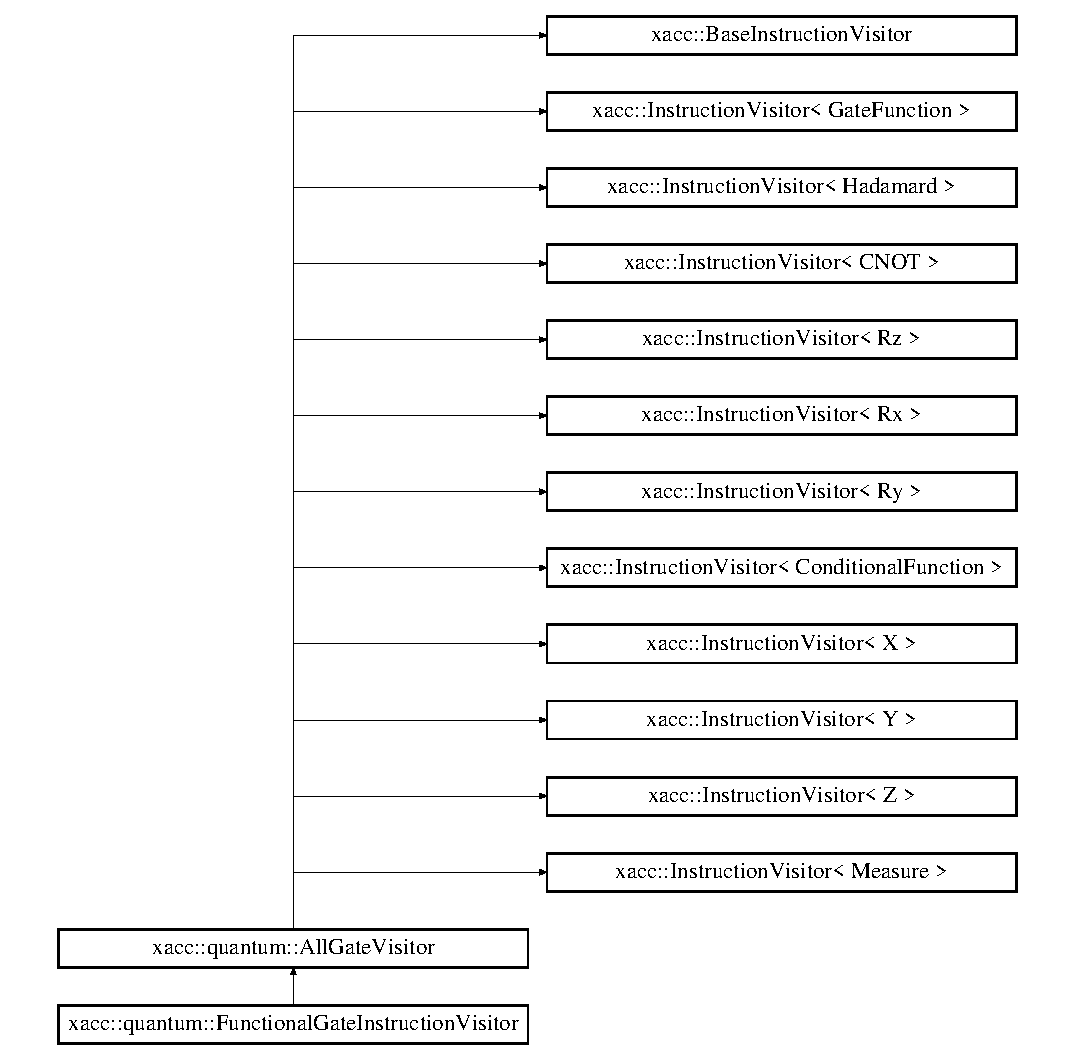
\includegraphics[height=12.000000cm]{a00031}
\end{center}
\end{figure}
\subsection*{Public Member Functions}
\begin{DoxyCompactItemize}
\item 
{\footnotesize template$<$typename HF , typename C\+NF , typename XF , typename YF , typename ZF , typename R\+XF , typename R\+YF , typename R\+ZF , typename MF , typename CF $>$ }\\{\bfseries Functional\+Gate\+Instruction\+Visitor} (HF h, C\+NF cn, XF x, YF y, ZF z, R\+XF rx, R\+YF ry, R\+ZF rz, MF m, CF c)\hypertarget{a00031_ab9e838d9bedab46a5ea54c9a0b99ef8a}{}\label{a00031_ab9e838d9bedab46a5ea54c9a0b99ef8a}

\item 
void {\bfseries visit} (\hyperlink{a00036}{Hadamard} \&h)\hypertarget{a00031_ac5245d34429dc112e7cd0e371108fcb5}{}\label{a00031_ac5245d34429dc112e7cd0e371108fcb5}

\item 
void {\bfseries visit} (\hyperlink{a00019}{C\+N\+OT} \&cn)\hypertarget{a00031_ad4eddafe8ca3906cd4aa5b98087a789a}{}\label{a00031_ad4eddafe8ca3906cd4aa5b98087a789a}

\item 
void {\bfseries visit} (\hyperlink{a00070}{X} \&x)\hypertarget{a00031_ac5d184daee7e755c9ede67b34bc2d091}{}\label{a00031_ac5d184daee7e755c9ede67b34bc2d091}

\item 
void {\bfseries visit} (\hyperlink{a00075}{Y} \&y)\hypertarget{a00031_a11dfa753a155346a45d7116a78c8f39f}{}\label{a00031_a11dfa753a155346a45d7116a78c8f39f}

\item 
void {\bfseries visit} (\hyperlink{a00076}{Z} \&z)\hypertarget{a00031_a4baf19da581fa9875739a227aba9cf60}{}\label{a00031_a4baf19da581fa9875739a227aba9cf60}

\item 
void {\bfseries visit} (\hyperlink{a00045}{Measure} \&m)\hypertarget{a00031_ad946faf8e2b6eff3e9e142907ec8e05a}{}\label{a00031_ad946faf8e2b6eff3e9e142907ec8e05a}

\item 
void {\bfseries visit} (\hyperlink{a00021}{Conditional\+Function} \&c)\hypertarget{a00031_a5cdb38902c241e7ae672a2631f1d61f3}{}\label{a00031_a5cdb38902c241e7ae672a2631f1d61f3}

\item 
void {\bfseries visit} (\hyperlink{a00061}{Rx} \&rx)\hypertarget{a00031_a6eb99e4b488773c750b7d9734ac1e885}{}\label{a00031_a6eb99e4b488773c750b7d9734ac1e885}

\item 
void {\bfseries visit} (\hyperlink{a00062}{Ry} \&ry)\hypertarget{a00031_aa22aad7b316386f5ef35672337c05ffc}{}\label{a00031_aa22aad7b316386f5ef35672337c05ffc}

\item 
void {\bfseries visit} (\hyperlink{a00063}{Rz} \&rz)\hypertarget{a00031_a8857ecf8f8f1b6143da8f31a722fe03e}{}\label{a00031_a8857ecf8f8f1b6143da8f31a722fe03e}

\item 
void {\bfseries visit} (\hyperlink{a00032}{Gate\+Function} \&f)\hypertarget{a00031_ad7d15225cf258fe59660ba828baff357}{}\label{a00031_ad7d15225cf258fe59660ba828baff357}

\end{DoxyCompactItemize}
\subsection*{Protected Attributes}
\begin{DoxyCompactItemize}
\item 
std\+::function$<$ void(\hyperlink{a00036}{Hadamard} \&)$>$ {\bfseries h\+Action}\hypertarget{a00031_a02f1401c9b0d1da801027f3bc0b5227e}{}\label{a00031_a02f1401c9b0d1da801027f3bc0b5227e}

\item 
std\+::function$<$ void(\hyperlink{a00019}{C\+N\+OT} \&)$>$ {\bfseries cnot\+Action}\hypertarget{a00031_a4d6bd8c2fd1af775ed08946942f60a0b}{}\label{a00031_a4d6bd8c2fd1af775ed08946942f60a0b}

\item 
std\+::function$<$ void(\hyperlink{a00070}{X} \&)$>$ {\bfseries x\+Action}\hypertarget{a00031_a9e0295434a2224b776609b057147a9af}{}\label{a00031_a9e0295434a2224b776609b057147a9af}

\item 
std\+::function$<$ void(\hyperlink{a00075}{Y} \&)$>$ {\bfseries y\+Action}\hypertarget{a00031_ae78f91a5cc9a7006f6bb1acee1c00501}{}\label{a00031_ae78f91a5cc9a7006f6bb1acee1c00501}

\item 
std\+::function$<$ void(\hyperlink{a00076}{Z} \&)$>$ {\bfseries z\+Action}\hypertarget{a00031_ae197f358e3d0777feb3656455e2ee672}{}\label{a00031_ae197f358e3d0777feb3656455e2ee672}

\item 
std\+::function$<$ void(\hyperlink{a00045}{Measure} \&)$>$ {\bfseries measure\+Action}\hypertarget{a00031_a239748abedd67c7b30cad12e545d1926}{}\label{a00031_a239748abedd67c7b30cad12e545d1926}

\item 
std\+::function$<$ void(\hyperlink{a00021}{Conditional\+Function} \&)$>$ {\bfseries cond\+Action}\hypertarget{a00031_a5c0595a70b1f7ae50f3e29a985e249e9}{}\label{a00031_a5c0595a70b1f7ae50f3e29a985e249e9}

\item 
std\+::function$<$ void(\hyperlink{a00061}{Rx} \&)$>$ {\bfseries rx\+Action}\hypertarget{a00031_ab79bb3eb3050d1c599061863bb2e219e}{}\label{a00031_ab79bb3eb3050d1c599061863bb2e219e}

\item 
std\+::function$<$ void(\hyperlink{a00062}{Ry} \&)$>$ {\bfseries ry\+Action}\hypertarget{a00031_a229b7d9aae52638c6eff04bd16bb9973}{}\label{a00031_a229b7d9aae52638c6eff04bd16bb9973}

\item 
std\+::function$<$ void(\hyperlink{a00063}{Rz} \&)$>$ {\bfseries rz\+Action}\hypertarget{a00031_a586ab5721150c67ad3ced46e2a236b44}{}\label{a00031_a586ab5721150c67ad3ced46e2a236b44}

\end{DoxyCompactItemize}


The documentation for this class was generated from the following file\+:\begin{DoxyCompactItemize}
\item 
Functional\+Gate\+Instruction\+Visitor.\+hpp\end{DoxyCompactItemize}

\hypertarget{a00032}{}\section{Accelerator\+Buffer Class Reference}
\label{a00032}\index{Accelerator\+Buffer@{Accelerator\+Buffer}}


{\ttfamily \#include $<$Accelerator\+Buffer.\+hpp$>$}

Inheritance diagram for Accelerator\+Buffer\+:\begin{figure}[H]
\begin{center}
\leavevmode
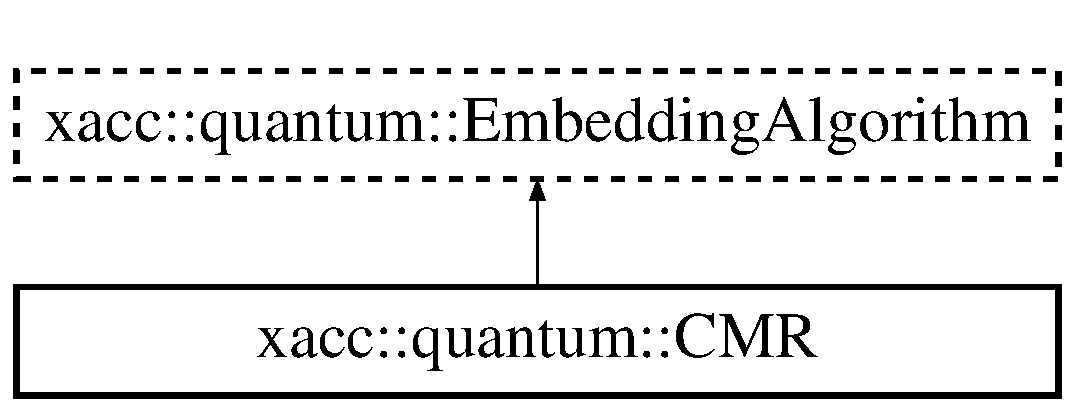
\includegraphics[height=2.000000cm]{a00032}
\end{center}
\end{figure}
\subsection*{Public Member Functions}
\begin{DoxyCompactItemize}
\item 
{\bfseries Accelerator\+Buffer} (const std\+::string \&str)\hypertarget{a00032_a5115079c3f3f8d32e713f78a91c93a7a}{}\label{a00032_a5115079c3f3f8d32e713f78a91c93a7a}

\item 
{\bfseries Accelerator\+Buffer} (const std\+::string \&str, const int N)\hypertarget{a00032_a6947082735241791c5170d677042da4a}{}\label{a00032_a6947082735241791c5170d677042da4a}

\item 
{\footnotesize template$<$typename... Indices$>$ }\\{\bfseries Accelerator\+Buffer} (const std\+::string \&str, int first\+Index, Indices...\+indices)\hypertarget{a00032_afe8b2a7e0b7b7992f45fe7021d106b66}{}\label{a00032_afe8b2a7e0b7b7992f45fe7021d106b66}

\item 
int {\bfseries size} ()\hypertarget{a00032_a249eae9f3b83072e5b101ba23f900e81}{}\label{a00032_a249eae9f3b83072e5b101ba23f900e81}

\item 
std\+::string {\bfseries name} ()\hypertarget{a00032_a3373218e4d430d061ba75135bf14ede3}{}\label{a00032_a3373218e4d430d061ba75135bf14ede3}

\item 
void {\bfseries reset\+Buffer} ()\hypertarget{a00032_aa5080c9a975871858b39d3394e867e77}{}\label{a00032_aa5080c9a975871858b39d3394e867e77}

\item 
void {\bfseries update\+Bit} (const int idx, int zero\+Or\+One)\hypertarget{a00032_a689855524e630049db6120a1493a3c45}{}\label{a00032_a689855524e630049db6120a1493a3c45}

\item 
Accelerator\+Bit\+State {\bfseries get\+Accelerator\+Bit\+State} (const int idx)\hypertarget{a00032_a29ece4f7b671308b89c06f3ac8e74b9e}{}\label{a00032_a29ece4f7b671308b89c06f3ac8e74b9e}

\item 
virtual void {\bfseries print} ()\hypertarget{a00032_a3776733a3196bca276988d4cc50a135a}{}\label{a00032_a3776733a3196bca276988d4cc50a135a}

\item 
virtual void {\bfseries print} (std\+::ostream \&stream)\hypertarget{a00032_a6f2cf905960a528fc829904a3c176c6e}{}\label{a00032_a6f2cf905960a528fc829904a3c176c6e}

\end{DoxyCompactItemize}
\subsection*{Protected Attributes}
\begin{DoxyCompactItemize}
\item 
std\+::string {\bfseries buffer\+Id}\hypertarget{a00032_adca17dc5025c067a927aefd6a5cbe51b}{}\label{a00032_adca17dc5025c067a927aefd6a5cbe51b}

\item 
std\+::vector$<$ \hyperlink{a00031}{Accelerator\+Bit} $>$ {\bfseries bits}\hypertarget{a00032_a36b3300cbada4e54e9e68d1c7c135c9b}{}\label{a00032_a36b3300cbada4e54e9e68d1c7c135c9b}

\end{DoxyCompactItemize}


\subsection{Detailed Description}
\begin{DoxyAuthor}{Author}
Alex Mc\+Caskey 
\end{DoxyAuthor}


The documentation for this class was generated from the following file\+:\begin{DoxyCompactItemize}
\item 
Accelerator\+Buffer.\+hpp\end{DoxyCompactItemize}

\hypertarget{a00033}{}\section{xacc\+:\+:quantum\+:\+:C\+N\+OT Class Reference}
\label{a00033}\index{xacc\+::quantum\+::\+C\+N\+OT@{xacc\+::quantum\+::\+C\+N\+OT}}
Inheritance diagram for xacc\+:\+:quantum\+:\+:C\+N\+OT\+:\begin{figure}[H]
\begin{center}
\leavevmode
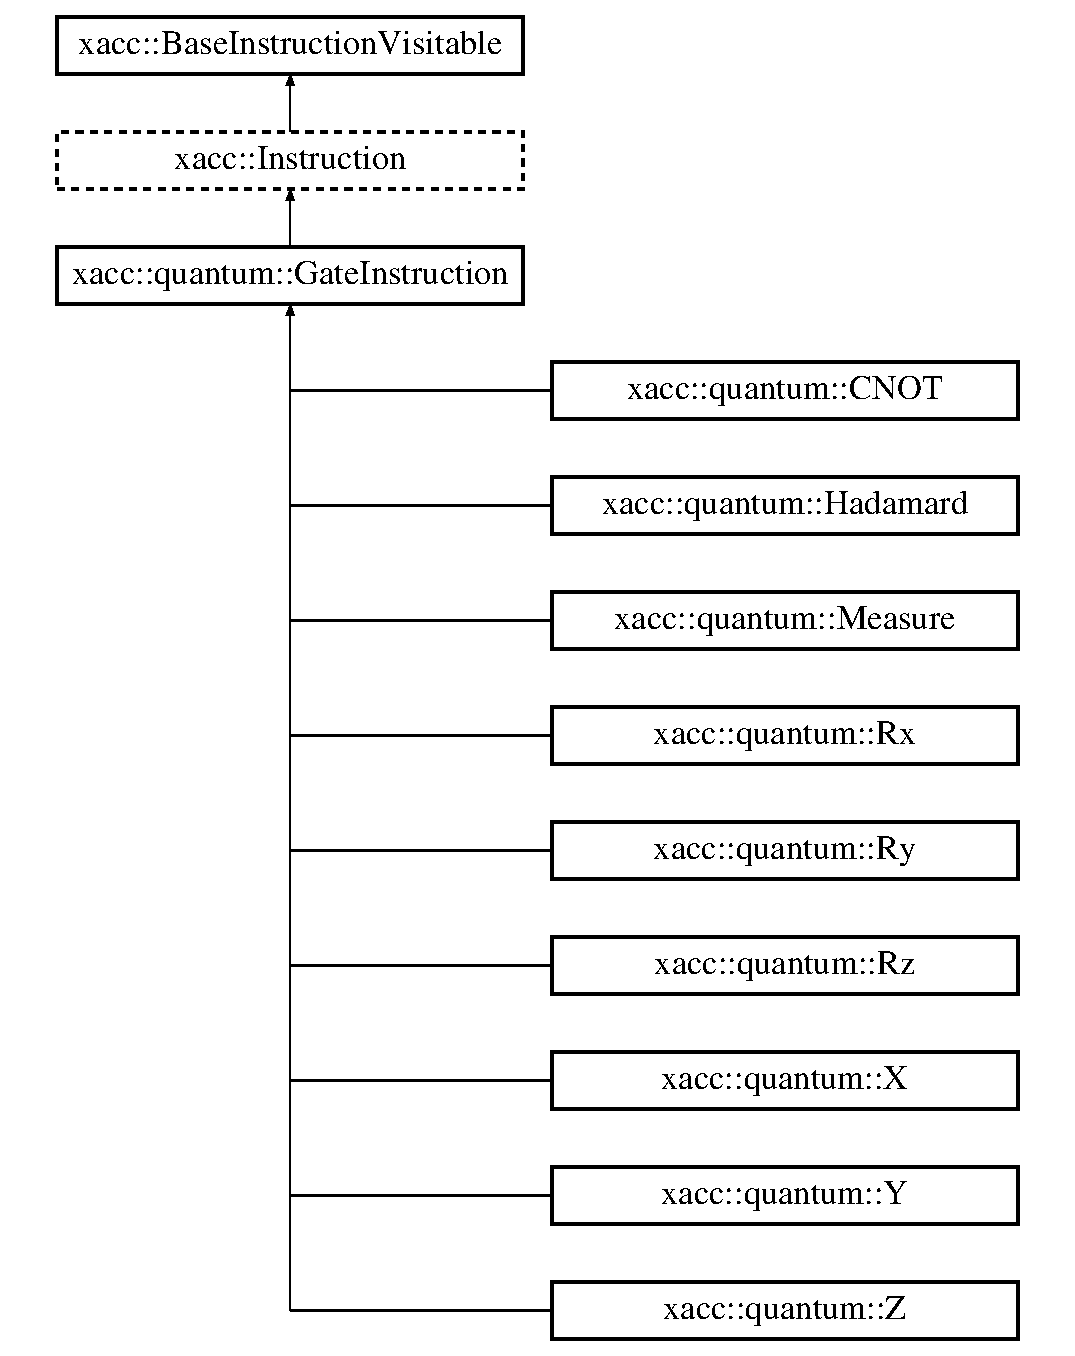
\includegraphics[height=4.000000cm]{a00033}
\end{center}
\end{figure}
\subsection*{Public Member Functions}
\begin{DoxyCompactItemize}
\item 
{\bfseries C\+N\+OT} (std\+::vector$<$ int $>$ \hyperlink{a00062_a2a56be6c2519ea65df4d06f4abae1393}{qbits})\hypertarget{a00033_ad3d460779a27affa317dd4f3a88268b3}{}\label{a00033_ad3d460779a27affa317dd4f3a88268b3}

\item 
{\bfseries C\+N\+OT} (int srcqbit, int tgtqbit)\hypertarget{a00033_a15efcb44477dde4b6151fe1776a73ddc}{}\label{a00033_a15efcb44477dde4b6151fe1776a73ddc}

\end{DoxyCompactItemize}
\subsection*{Additional Inherited Members}


The documentation for this class was generated from the following files\+:\begin{DoxyCompactItemize}
\item 
C\+N\+O\+T.\+hpp\item 
C\+N\+O\+T.\+cpp\end{DoxyCompactItemize}

\hypertarget{a00034}{}\section{xacc\+:\+:quantum\+:\+:D\+W\+Q\+M\+I\+Compiler Class Reference}
\label{a00034}\index{xacc\+::quantum\+::\+D\+W\+Q\+M\+I\+Compiler@{xacc\+::quantum\+::\+D\+W\+Q\+M\+I\+Compiler}}


{\ttfamily \#include $<$D\+W\+Q\+M\+I\+Compiler.\+hpp$>$}

Inheritance diagram for xacc\+:\+:quantum\+:\+:D\+W\+Q\+M\+I\+Compiler\+:\begin{figure}[H]
\begin{center}
\leavevmode
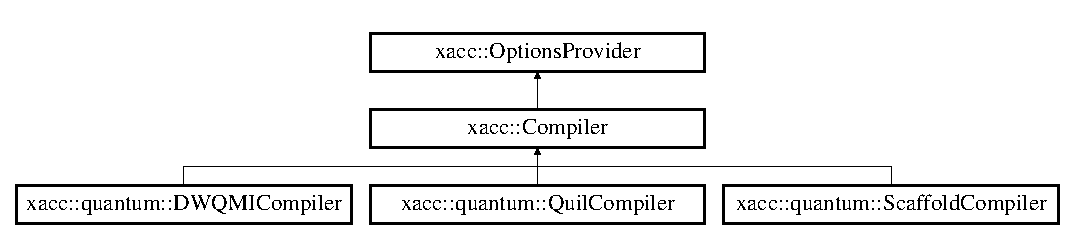
\includegraphics[height=3.000000cm]{a00034}
\end{center}
\end{figure}
\subsection*{Public Member Functions}
\begin{DoxyCompactItemize}
\item 
\hyperlink{a00034_a1f285f3eaec09363d9439676dbdfbd6a}{D\+W\+Q\+M\+I\+Compiler} ()
\item 
virtual std\+::shared\+\_\+ptr$<$ \hyperlink{a00050}{xacc\+::\+IR} $>$ \hyperlink{a00034_a0df05642f1a6fd44ce7f1c0396d50c9c}{compile} (const std\+::string \&src, std\+::shared\+\_\+ptr$<$ \hyperlink{a00011}{Accelerator} $>$ acc)
\item 
virtual std\+::shared\+\_\+ptr$<$ \hyperlink{a00050}{xacc\+::\+IR} $>$ \hyperlink{a00034_aa22591343b5509bf2c3a5820130ba906}{compile} (const std\+::string \&src)
\item 
virtual const std\+::string \hyperlink{a00034_aed42de96f8e0dd94b6de183f28aee419}{get\+Name} ()
\item 
virtual std\+::shared\+\_\+ptr$<$ options\+\_\+description $>$ \hyperlink{a00034_a0851334cc33b5b1da2694150a0a1a43c}{get\+Options} ()
\item 
virtual const std\+::string \hyperlink{a00034_a56a345539665099329209b3b5f6810c9}{translate} (const std\+::string \&buffer\+Variable, std\+::shared\+\_\+ptr$<$ \hyperlink{a00038}{Function} $>$ function)
\item 
virtual \hyperlink{a00034_a86f9135f7dc1c3246970e2a7f6540b5c}{$\sim$\+D\+W\+Q\+M\+I\+Compiler} ()
\end{DoxyCompactItemize}
\subsection*{Static Public Member Functions}
\begin{DoxyCompactItemize}
\item 
static void \hyperlink{a00034_a421daa5286f31e2b5ab4c141a34c94cd}{register\+Compiler} ()
\end{DoxyCompactItemize}
\subsection*{Additional Inherited Members}


\subsection{Detailed Description}
The \hyperlink{a00034}{D\+W\+Q\+M\+I\+Compiler} is an X\+A\+CC \hyperlink{a00023}{Compiler} that compiles D-\/\+Wave quantum machine instructions to produce an appropriate Ising form for execution on the D-\/\+Wave Q\+PU.

This compilation leverages X\+A\+CC Embedding\+Algorithms to compute the minor graph embedding represented by the input source kernel code to output the embedded Ising graph for D-\/\+Wave execution. 

\subsection{Constructor \& Destructor Documentation}
\index{xacc\+::quantum\+::\+D\+W\+Q\+M\+I\+Compiler@{xacc\+::quantum\+::\+D\+W\+Q\+M\+I\+Compiler}!D\+W\+Q\+M\+I\+Compiler@{D\+W\+Q\+M\+I\+Compiler}}
\index{D\+W\+Q\+M\+I\+Compiler@{D\+W\+Q\+M\+I\+Compiler}!xacc\+::quantum\+::\+D\+W\+Q\+M\+I\+Compiler@{xacc\+::quantum\+::\+D\+W\+Q\+M\+I\+Compiler}}
\subsubsection[{\texorpdfstring{D\+W\+Q\+M\+I\+Compiler()}{DWQMICompiler()}}]{\setlength{\rightskip}{0pt plus 5cm}xacc\+::quantum\+::\+D\+W\+Q\+M\+I\+Compiler\+::\+D\+W\+Q\+M\+I\+Compiler (
\begin{DoxyParamCaption}
{}
\end{DoxyParamCaption}
)\hspace{0.3cm}{\ttfamily [inline]}}\hypertarget{a00034_a1f285f3eaec09363d9439676dbdfbd6a}{}\label{a00034_a1f285f3eaec09363d9439676dbdfbd6a}
The \hyperlink{a00023}{Compiler}. \index{xacc\+::quantum\+::\+D\+W\+Q\+M\+I\+Compiler@{xacc\+::quantum\+::\+D\+W\+Q\+M\+I\+Compiler}!````~D\+W\+Q\+M\+I\+Compiler@{$\sim$\+D\+W\+Q\+M\+I\+Compiler}}
\index{````~D\+W\+Q\+M\+I\+Compiler@{$\sim$\+D\+W\+Q\+M\+I\+Compiler}!xacc\+::quantum\+::\+D\+W\+Q\+M\+I\+Compiler@{xacc\+::quantum\+::\+D\+W\+Q\+M\+I\+Compiler}}
\subsubsection[{\texorpdfstring{$\sim$\+D\+W\+Q\+M\+I\+Compiler()}{~DWQMICompiler()}}]{\setlength{\rightskip}{0pt plus 5cm}virtual xacc\+::quantum\+::\+D\+W\+Q\+M\+I\+Compiler\+::$\sim$\+D\+W\+Q\+M\+I\+Compiler (
\begin{DoxyParamCaption}
{}
\end{DoxyParamCaption}
)\hspace{0.3cm}{\ttfamily [inline]}, {\ttfamily [virtual]}}\hypertarget{a00034_a86f9135f7dc1c3246970e2a7f6540b5c}{}\label{a00034_a86f9135f7dc1c3246970e2a7f6540b5c}
The destructor 

\subsection{Member Function Documentation}
\index{xacc\+::quantum\+::\+D\+W\+Q\+M\+I\+Compiler@{xacc\+::quantum\+::\+D\+W\+Q\+M\+I\+Compiler}!compile@{compile}}
\index{compile@{compile}!xacc\+::quantum\+::\+D\+W\+Q\+M\+I\+Compiler@{xacc\+::quantum\+::\+D\+W\+Q\+M\+I\+Compiler}}
\subsubsection[{\texorpdfstring{compile(const std\+::string \&src, std\+::shared\+\_\+ptr$<$ Accelerator $>$ acc)}{compile(const std::string \&src, std::shared\_ptr< Accelerator > acc)}}]{\setlength{\rightskip}{0pt plus 5cm}std\+::shared\+\_\+ptr$<$ {\bf IR} $>$ xacc\+::quantum\+::\+D\+W\+Q\+M\+I\+Compiler\+::compile (
\begin{DoxyParamCaption}
\item[{const std\+::string \&}]{src, }
\item[{std\+::shared\+\_\+ptr$<$ {\bf Accelerator} $>$}]{acc}
\end{DoxyParamCaption}
)\hspace{0.3cm}{\ttfamily [virtual]}}\hypertarget{a00034_a0df05642f1a6fd44ce7f1c0396d50c9c}{}\label{a00034_a0df05642f1a6fd44ce7f1c0396d50c9c}
Compile the given kernel code for the given D-\/\+Wave \hyperlink{a00011}{Accelerator}.


\begin{DoxyParams}{Parameters}
{\em src} & The Q\+MI source code \\
\hline
{\em acc} & Reference to the D-\/\+Wave \hyperlink{a00011}{Accelerator} \\
\hline
\end{DoxyParams}
\begin{DoxyReturn}{Returns}

\end{DoxyReturn}


Implements \hyperlink{a00023_a546a40c95bb93af6a0c0ac48dbeaffc8}{xacc\+::\+Compiler}.

\index{xacc\+::quantum\+::\+D\+W\+Q\+M\+I\+Compiler@{xacc\+::quantum\+::\+D\+W\+Q\+M\+I\+Compiler}!compile@{compile}}
\index{compile@{compile}!xacc\+::quantum\+::\+D\+W\+Q\+M\+I\+Compiler@{xacc\+::quantum\+::\+D\+W\+Q\+M\+I\+Compiler}}
\subsubsection[{\texorpdfstring{compile(const std\+::string \&src)}{compile(const std::string \&src)}}]{\setlength{\rightskip}{0pt plus 5cm}std\+::shared\+\_\+ptr$<$ {\bf IR} $>$ xacc\+::quantum\+::\+D\+W\+Q\+M\+I\+Compiler\+::compile (
\begin{DoxyParamCaption}
\item[{const std\+::string \&}]{src}
\end{DoxyParamCaption}
)\hspace{0.3cm}{\ttfamily [virtual]}}\hypertarget{a00034_aa22591343b5509bf2c3a5820130ba906}{}\label{a00034_aa22591343b5509bf2c3a5820130ba906}
This method is not implemented -\/ we must always have D-\/\+Wave \hyperlink{a00011}{Accelerator} connectivity information for compilation.

\begin{DoxyReturn}{Returns}

\end{DoxyReturn}


Implements \hyperlink{a00023_a9092f5f779b570c91569b59621280c04}{xacc\+::\+Compiler}.

\index{xacc\+::quantum\+::\+D\+W\+Q\+M\+I\+Compiler@{xacc\+::quantum\+::\+D\+W\+Q\+M\+I\+Compiler}!get\+Name@{get\+Name}}
\index{get\+Name@{get\+Name}!xacc\+::quantum\+::\+D\+W\+Q\+M\+I\+Compiler@{xacc\+::quantum\+::\+D\+W\+Q\+M\+I\+Compiler}}
\subsubsection[{\texorpdfstring{get\+Name()}{getName()}}]{\setlength{\rightskip}{0pt plus 5cm}virtual const std\+::string xacc\+::quantum\+::\+D\+W\+Q\+M\+I\+Compiler\+::get\+Name (
\begin{DoxyParamCaption}
{}
\end{DoxyParamCaption}
)\hspace{0.3cm}{\ttfamily [inline]}, {\ttfamily [virtual]}}\hypertarget{a00034_aed42de96f8e0dd94b6de183f28aee419}{}\label{a00034_aed42de96f8e0dd94b6de183f28aee419}
Return the name of this \hyperlink{a00023}{Compiler} \begin{DoxyReturn}{Returns}
name \hyperlink{a00023}{Compiler} name 
\end{DoxyReturn}


Implements \hyperlink{a00023_a87fca9100e6462122f5b687c3a0fb3fb}{xacc\+::\+Compiler}.

\index{xacc\+::quantum\+::\+D\+W\+Q\+M\+I\+Compiler@{xacc\+::quantum\+::\+D\+W\+Q\+M\+I\+Compiler}!get\+Options@{get\+Options}}
\index{get\+Options@{get\+Options}!xacc\+::quantum\+::\+D\+W\+Q\+M\+I\+Compiler@{xacc\+::quantum\+::\+D\+W\+Q\+M\+I\+Compiler}}
\subsubsection[{\texorpdfstring{get\+Options()}{getOptions()}}]{\setlength{\rightskip}{0pt plus 5cm}virtual std\+::shared\+\_\+ptr$<$options\+\_\+description$>$ xacc\+::quantum\+::\+D\+W\+Q\+M\+I\+Compiler\+::get\+Options (
\begin{DoxyParamCaption}
{}
\end{DoxyParamCaption}
)\hspace{0.3cm}{\ttfamily [inline]}, {\ttfamily [virtual]}}\hypertarget{a00034_a0851334cc33b5b1da2694150a0a1a43c}{}\label{a00034_a0851334cc33b5b1da2694150a0a1a43c}
Return the command line options for this compiler

\begin{DoxyReturn}{Returns}
options Description of command line options. 
\end{DoxyReturn}


Reimplemented from \hyperlink{a00023_a9f5a8965c9c2dd895016d18264ebbe92}{xacc\+::\+Compiler}.

\index{xacc\+::quantum\+::\+D\+W\+Q\+M\+I\+Compiler@{xacc\+::quantum\+::\+D\+W\+Q\+M\+I\+Compiler}!register\+Compiler@{register\+Compiler}}
\index{register\+Compiler@{register\+Compiler}!xacc\+::quantum\+::\+D\+W\+Q\+M\+I\+Compiler@{xacc\+::quantum\+::\+D\+W\+Q\+M\+I\+Compiler}}
\subsubsection[{\texorpdfstring{register\+Compiler()}{registerCompiler()}}]{\setlength{\rightskip}{0pt plus 5cm}static void xacc\+::quantum\+::\+D\+W\+Q\+M\+I\+Compiler\+::register\+Compiler (
\begin{DoxyParamCaption}
{}
\end{DoxyParamCaption}
)\hspace{0.3cm}{\ttfamily [inline]}, {\ttfamily [static]}}\hypertarget{a00034_a421daa5286f31e2b5ab4c141a34c94cd}{}\label{a00034_a421daa5286f31e2b5ab4c141a34c94cd}
Register this \hyperlink{a00023}{Compiler} with the framework. \index{xacc\+::quantum\+::\+D\+W\+Q\+M\+I\+Compiler@{xacc\+::quantum\+::\+D\+W\+Q\+M\+I\+Compiler}!translate@{translate}}
\index{translate@{translate}!xacc\+::quantum\+::\+D\+W\+Q\+M\+I\+Compiler@{xacc\+::quantum\+::\+D\+W\+Q\+M\+I\+Compiler}}
\subsubsection[{\texorpdfstring{translate(const std\+::string \&buffer\+Variable, std\+::shared\+\_\+ptr$<$ Function $>$ function)}{translate(const std::string \&bufferVariable, std::shared\_ptr< Function > function)}}]{\setlength{\rightskip}{0pt plus 5cm}virtual const std\+::string xacc\+::quantum\+::\+D\+W\+Q\+M\+I\+Compiler\+::translate (
\begin{DoxyParamCaption}
\item[{const std\+::string \&}]{buffer\+Variable, }
\item[{std\+::shared\+\_\+ptr$<$ {\bf Function} $>$}]{function}
\end{DoxyParamCaption}
)\hspace{0.3cm}{\ttfamily [inline]}, {\ttfamily [virtual]}}\hypertarget{a00034_a56a345539665099329209b3b5f6810c9}{}\label{a00034_a56a345539665099329209b3b5f6810c9}
We don\textquotesingle{}t allow translations for the DW \hyperlink{a00023}{Compiler}. 
\begin{DoxyParams}{Parameters}
{\em buffer\+Variable} & \\
\hline
{\em function} & \\
\hline
\end{DoxyParams}
\begin{DoxyReturn}{Returns}

\end{DoxyReturn}


Implements \hyperlink{a00023_aeedbe58a33fed29e4d7694ae743e25e7}{xacc\+::\+Compiler}.



The documentation for this class was generated from the following files\+:\begin{DoxyCompactItemize}
\item 
D\+W\+Q\+M\+I\+Compiler.\+hpp\item 
D\+W\+Q\+M\+I\+Compiler.\+cpp\end{DoxyCompactItemize}

\hypertarget{a00035}{}\section{xacc\+:\+:quantum\+:\+:D\+W\+Solver Struct Reference}
\label{a00035}\index{xacc\+::quantum\+::\+D\+W\+Solver@{xacc\+::quantum\+::\+D\+W\+Solver}}


{\ttfamily \#include $<$D\+W\+Accelerator.\+hpp$>$}

\subsection*{Public Attributes}
\begin{DoxyCompactItemize}
\item 
std\+::string {\bfseries name}\hypertarget{a00035_a8a5b629dc83790a855d429c82266b772}{}\label{a00035_a8a5b629dc83790a855d429c82266b772}

\item 
std\+::string {\bfseries description}\hypertarget{a00035_a9bb9449a6ea09e11892f910a4bfd2e08}{}\label{a00035_a9bb9449a6ea09e11892f910a4bfd2e08}

\item 
double {\bfseries j\+Range\+Min}\hypertarget{a00035_a45fc23af53f44759afec0257d9878ba0}{}\label{a00035_a45fc23af53f44759afec0257d9878ba0}

\item 
double {\bfseries j\+Range\+Max}\hypertarget{a00035_aa881af1344ff55a4991c152f768ed9d6}{}\label{a00035_aa881af1344ff55a4991c152f768ed9d6}

\item 
double {\bfseries h\+Range\+Min}\hypertarget{a00035_abf475612dac8f64a7f88cfa976c393f0}{}\label{a00035_abf475612dac8f64a7f88cfa976c393f0}

\item 
double {\bfseries h\+Range\+Max}\hypertarget{a00035_a13dd875ceb06c7545fe20cde15ffac70}{}\label{a00035_a13dd875ceb06c7545fe20cde15ffac70}

\item 
int {\bfseries n\+Qubits}\hypertarget{a00035_a2908c913f5c5e3ade6551056aaadafbf}{}\label{a00035_a2908c913f5c5e3ade6551056aaadafbf}

\item 
std\+::vector$<$ std\+::pair$<$ int, int $>$ $>$ {\bfseries edges}\hypertarget{a00035_ae02cbfe68c982e50e80bcd2612c8c148}{}\label{a00035_ae02cbfe68c982e50e80bcd2612c8c148}

\end{DoxyCompactItemize}


\subsection{Detailed Description}
Wrapper for information related to the remote D-\/\+Wave solver. 

The documentation for this struct was generated from the following file\+:\begin{DoxyCompactItemize}
\item 
D\+W\+Accelerator.\+hpp\end{DoxyCompactItemize}

\hypertarget{a00036}{}\section{fire\+:\+:array\+\_\+size$<$ std\+:\+:array$<$ T, N $>$ $>$ Struct Template Reference}
\label{a00036}\index{fire\+::array\+\_\+size$<$ std\+::array$<$ T, N $>$ $>$@{fire\+::array\+\_\+size$<$ std\+::array$<$ T, N $>$ $>$}}
\subsection*{Static Public Attributes}
\begin{DoxyCompactItemize}
\item 
static const size\+\_\+t {\bfseries value} = N\hypertarget{a00036_ab92887f3c176f5d68d76c67b4db2f112}{}\label{a00036_ab92887f3c176f5d68d76c67b4db2f112}

\end{DoxyCompactItemize}


The documentation for this struct was generated from the following file\+:\begin{DoxyCompactItemize}
\item 
Tensor\+Utils.\+hpp\end{DoxyCompactItemize}

\hypertarget{a00037}{}\section{Generic\+Value$<$ Encoding, Allocator $>$\+:\+:Array\+Data Struct Reference}
\label{a00037}\index{Generic\+Value$<$ Encoding, Allocator $>$\+::\+Array\+Data@{Generic\+Value$<$ Encoding, Allocator $>$\+::\+Array\+Data}}
\subsection*{Public Attributes}
\begin{DoxyCompactItemize}
\item 
\hyperlink{a00677_a5ed6e6e67250fadbd041127e6386dcb5}{Size\+Type} {\bfseries size}\hypertarget{a00037_a5306856f64aea8ec53abf263ed2a35e2}{}\label{a00037_a5306856f64aea8ec53abf263ed2a35e2}

\item 
\hyperlink{a00677_a5ed6e6e67250fadbd041127e6386dcb5}{Size\+Type} {\bfseries capacity}\hypertarget{a00037_a0c6fe03c00e13d14b95abd31048aa1f5}{}\label{a00037_a0c6fe03c00e13d14b95abd31048aa1f5}

\item 
\hyperlink{a00130}{Generic\+Value} $\ast$ {\bfseries elements}\hypertarget{a00037_a86df976cb6f65924aca20eb9bd35553e}{}\label{a00037_a86df976cb6f65924aca20eb9bd35553e}

\end{DoxyCompactItemize}


The documentation for this struct was generated from the following file\+:\begin{DoxyCompactItemize}
\item 
\hyperlink{a00473}{document.\+h}\end{DoxyCompactItemize}

\hypertarget{a00038}{}\section{nlohmann\+:\+:basic\+\_\+json$<$ Object\+Type, Array\+Type, String\+Type, Boolean\+Type, Number\+Integer\+Type, Number\+Unsigned\+Type, Number\+Float\+Type, Allocator\+Type $>$\+:\+:const\+\_\+iterator Class Reference}
\label{a00038}\index{nlohmann\+::basic\+\_\+json$<$ Object\+Type, Array\+Type, String\+Type, Boolean\+Type, Number\+Integer\+Type, Number\+Unsigned\+Type, Number\+Float\+Type, Allocator\+Type $>$\+::const\+\_\+iterator@{nlohmann\+::basic\+\_\+json$<$ Object\+Type, Array\+Type, String\+Type, Boolean\+Type, Number\+Integer\+Type, Number\+Unsigned\+Type, Number\+Float\+Type, Allocator\+Type $>$\+::const\+\_\+iterator}}


a const random access iterator for the \hyperlink{a00025}{basic\+\_\+json} class  




{\ttfamily \#include $<$json.\+hpp$>$}

Inheritance diagram for nlohmann\+:\+:basic\+\_\+json$<$ Object\+Type, Array\+Type, String\+Type, Boolean\+Type, Number\+Integer\+Type, Number\+Unsigned\+Type, Number\+Float\+Type, Allocator\+Type $>$\+:\+:const\+\_\+iterator\+:\begin{figure}[H]
\begin{center}
\leavevmode
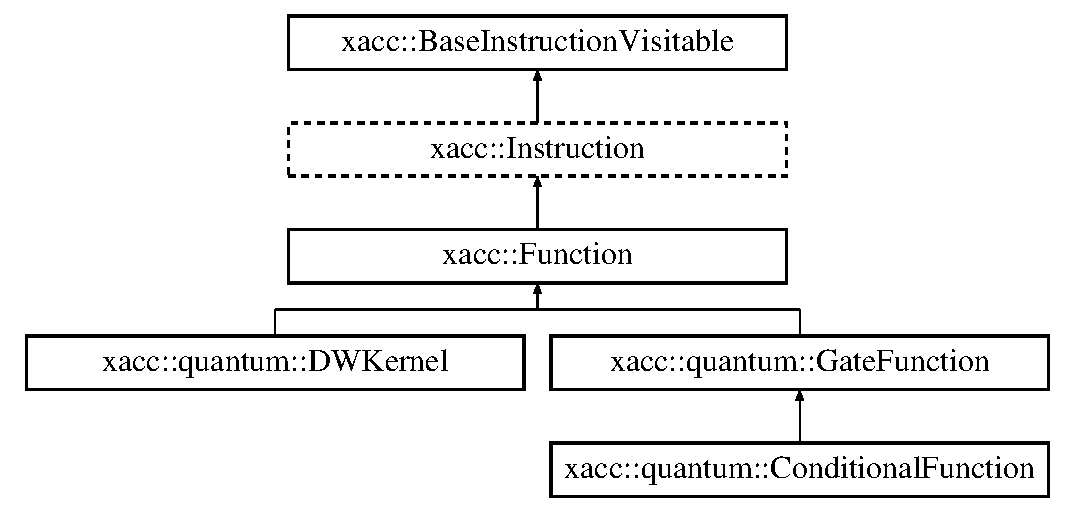
\includegraphics[height=1.705584cm]{a00038}
\end{center}
\end{figure}
\subsection*{Public Types}
\begin{DoxyCompactItemize}
\item 
using \hyperlink{a00038_a9ea0497199b1e96ce9cadd1f202ec343}{value\+\_\+type} = typename \hyperlink{a00025_ac8d45b57874b4a6e9c07f7d3b5daa1f9}{basic\+\_\+json\+::value\+\_\+type}\hypertarget{a00038_a9ea0497199b1e96ce9cadd1f202ec343}{}\label{a00038_a9ea0497199b1e96ce9cadd1f202ec343}

\begin{DoxyCompactList}\small\item\em the type of the values when the iterator is dereferenced \end{DoxyCompactList}\item 
using \hyperlink{a00038_a49d7c3e9ef3280df03052cce988b792f}{difference\+\_\+type} = typename \hyperlink{a00025_aec316934a555dd1acdd3600e5d4a4cdf}{basic\+\_\+json\+::difference\+\_\+type}\hypertarget{a00038_a49d7c3e9ef3280df03052cce988b792f}{}\label{a00038_a49d7c3e9ef3280df03052cce988b792f}

\begin{DoxyCompactList}\small\item\em a type to represent differences between iterators \end{DoxyCompactList}\item 
using \hyperlink{a00038_a1da96fc3054d547e7706d3a2f073f389}{pointer} = typename \hyperlink{a00025_a06efb200b69942eacd1ea22d0f6ccebb}{basic\+\_\+json\+::const\+\_\+pointer}\hypertarget{a00038_a1da96fc3054d547e7706d3a2f073f389}{}\label{a00038_a1da96fc3054d547e7706d3a2f073f389}

\begin{DoxyCompactList}\small\item\em defines a pointer to the type iterated over (value\+\_\+type) \end{DoxyCompactList}\item 
using \hyperlink{a00038_aefd248cac6493eed1e6ff53ba6a63eb2}{reference} = typename \hyperlink{a00025_af677a29b0e66edc9f66e5167e4667071}{basic\+\_\+json\+::const\+\_\+reference}\hypertarget{a00038_aefd248cac6493eed1e6ff53ba6a63eb2}{}\label{a00038_aefd248cac6493eed1e6ff53ba6a63eb2}

\begin{DoxyCompactList}\small\item\em defines a reference to the type iterated over (value\+\_\+type) \end{DoxyCompactList}\item 
using \hyperlink{a00038_a821560d64f50525162097f19b1392e7f}{iterator\+\_\+category} = std\+::bidirectional\+\_\+iterator\+\_\+tag\hypertarget{a00038_a821560d64f50525162097f19b1392e7f}{}\label{a00038_a821560d64f50525162097f19b1392e7f}

\begin{DoxyCompactList}\small\item\em the category of the iterator \end{DoxyCompactList}\end{DoxyCompactItemize}
\subsection*{Public Member Functions}
\begin{DoxyCompactItemize}
\item 
\hyperlink{a00038_ac6fdaff67857f82a623e5cc253917639}{const\+\_\+iterator} ()=default\hypertarget{a00038_ac6fdaff67857f82a623e5cc253917639}{}\label{a00038_ac6fdaff67857f82a623e5cc253917639}

\begin{DoxyCompactList}\small\item\em default constructor \end{DoxyCompactList}\item 
\hyperlink{a00038_a23de834b11bd895209aa65c100ab9ceb}{const\+\_\+iterator} (\hyperlink{a00038_a1da96fc3054d547e7706d3a2f073f389}{pointer} \hyperlink{a00025_ad25b2f8c21e241e2d63455537a9294ff}{object}) noexcept\hypertarget{a00038_a23de834b11bd895209aa65c100ab9ceb}{}\label{a00038_a23de834b11bd895209aa65c100ab9ceb}

\begin{DoxyCompactList}\small\item\em constructor for a given J\+S\+ON instance \end{DoxyCompactList}\item 
\hyperlink{a00038_a6b950c6bc081ac1ec1540ec05ceb2603}{const\+\_\+iterator} (const \hyperlink{a00079}{iterator} \&other) noexcept\hypertarget{a00038_a6b950c6bc081ac1ec1540ec05ceb2603}{}\label{a00038_a6b950c6bc081ac1ec1540ec05ceb2603}

\begin{DoxyCompactList}\small\item\em copy constructor given a nonconst iterator \end{DoxyCompactList}\item 
\hyperlink{a00038_a18c35a6735d3da96b4fc026421c05dd8}{const\+\_\+iterator} (const \hyperlink{a00038}{const\+\_\+iterator} \&other) noexcept\hypertarget{a00038_a18c35a6735d3da96b4fc026421c05dd8}{}\label{a00038_a18c35a6735d3da96b4fc026421c05dd8}

\begin{DoxyCompactList}\small\item\em copy constructor \end{DoxyCompactList}\item 
\hyperlink{a00038}{const\+\_\+iterator} \& \hyperlink{a00038_a5521515067b6597cb0b55a9c547a7a2b}{operator=} (\hyperlink{a00038}{const\+\_\+iterator} other) noexcept(                                       std\+::is\+\_\+nothrow\+\_\+move\+\_\+constructible$<$ \hyperlink{a00038_a1da96fc3054d547e7706d3a2f073f389}{pointer} $>$\+::\hyperlink{a00038_ac75e80d30b6169ee2a29ec93fb4d2acd}{value} and                                       std\+::is\+\_\+nothrow\+\_\+move\+\_\+assignable$<$ \hyperlink{a00038_a1da96fc3054d547e7706d3a2f073f389}{pointer} $>$\+::\hyperlink{a00038_ac75e80d30b6169ee2a29ec93fb4d2acd}{value} and                                       std\+::is\+\_\+nothrow\+\_\+move\+\_\+constructible$<$ internal\+\_\+iterator $>$\+::\hyperlink{a00038_ac75e80d30b6169ee2a29ec93fb4d2acd}{value} and                                       std\+::is\+\_\+nothrow\+\_\+move\+\_\+assignable$<$ internal\+\_\+iterator $>$\+::\hyperlink{a00038_ac75e80d30b6169ee2a29ec93fb4d2acd}{value}                       )\hypertarget{a00038_a5521515067b6597cb0b55a9c547a7a2b}{}\label{a00038_a5521515067b6597cb0b55a9c547a7a2b}

\begin{DoxyCompactList}\small\item\em copy assignment \end{DoxyCompactList}\item 
\hyperlink{a00038_aefd248cac6493eed1e6ff53ba6a63eb2}{reference} \hyperlink{a00038_ab3029a1a83cf46dc28ad443bbad0c74d}{operator$\ast$} () const \hypertarget{a00038_ab3029a1a83cf46dc28ad443bbad0c74d}{}\label{a00038_ab3029a1a83cf46dc28ad443bbad0c74d}

\begin{DoxyCompactList}\small\item\em return a reference to the value pointed to by the iterator \end{DoxyCompactList}\item 
\hyperlink{a00038_a1da96fc3054d547e7706d3a2f073f389}{pointer} \hyperlink{a00038_a8be837e4d902887676dd837abe9098d3}{operator-\/$>$} () const \hypertarget{a00038_a8be837e4d902887676dd837abe9098d3}{}\label{a00038_a8be837e4d902887676dd837abe9098d3}

\begin{DoxyCompactList}\small\item\em dereference the iterator \end{DoxyCompactList}\item 
\hyperlink{a00038}{const\+\_\+iterator} \hyperlink{a00038_a8dbaec5bf8ccba3225520356629061cb}{operator++} (int)\hypertarget{a00038_a8dbaec5bf8ccba3225520356629061cb}{}\label{a00038_a8dbaec5bf8ccba3225520356629061cb}

\begin{DoxyCompactList}\small\item\em post-\/increment (it++) \end{DoxyCompactList}\item 
\hyperlink{a00038}{const\+\_\+iterator} \& \hyperlink{a00038_a8fbb15efd97599209a7def77af8e748e}{operator++} ()\hypertarget{a00038_a8fbb15efd97599209a7def77af8e748e}{}\label{a00038_a8fbb15efd97599209a7def77af8e748e}

\begin{DoxyCompactList}\small\item\em pre-\/increment (++it) \end{DoxyCompactList}\item 
\hyperlink{a00038}{const\+\_\+iterator} \hyperlink{a00038_a6cab1c2ed7e2a014980e2a5717f43a64}{operator-\/-\/} (int)\hypertarget{a00038_a6cab1c2ed7e2a014980e2a5717f43a64}{}\label{a00038_a6cab1c2ed7e2a014980e2a5717f43a64}

\begin{DoxyCompactList}\small\item\em post-\/decrement (it--) \end{DoxyCompactList}\item 
\hyperlink{a00038}{const\+\_\+iterator} \& \hyperlink{a00038_adeb2ff3fdf3cc301b72db109934c9199}{operator-\/-\/} ()\hypertarget{a00038_adeb2ff3fdf3cc301b72db109934c9199}{}\label{a00038_adeb2ff3fdf3cc301b72db109934c9199}

\begin{DoxyCompactList}\small\item\em pre-\/decrement (--it) \end{DoxyCompactList}\item 
bool \hyperlink{a00038_ab4c0b9baaec9ebc4837158e272f6c803}{operator==} (const \hyperlink{a00038}{const\+\_\+iterator} \&other) const \hypertarget{a00038_ab4c0b9baaec9ebc4837158e272f6c803}{}\label{a00038_ab4c0b9baaec9ebc4837158e272f6c803}

\begin{DoxyCompactList}\small\item\em comparison\+: equal \end{DoxyCompactList}\item 
bool \hyperlink{a00038_a9e4c6e48e3c2f3ff357ef8215b8c8fca}{operator!=} (const \hyperlink{a00038}{const\+\_\+iterator} \&other) const \hypertarget{a00038_a9e4c6e48e3c2f3ff357ef8215b8c8fca}{}\label{a00038_a9e4c6e48e3c2f3ff357ef8215b8c8fca}

\begin{DoxyCompactList}\small\item\em comparison\+: not equal \end{DoxyCompactList}\item 
bool \hyperlink{a00038_a65f491b515e5967e9c0b40289e3c0ff3}{operator$<$} (const \hyperlink{a00038}{const\+\_\+iterator} \&other) const \hypertarget{a00038_a65f491b515e5967e9c0b40289e3c0ff3}{}\label{a00038_a65f491b515e5967e9c0b40289e3c0ff3}

\begin{DoxyCompactList}\small\item\em comparison\+: smaller \end{DoxyCompactList}\item 
bool \hyperlink{a00038_a6b682f09787eff62f03493d45aa05902}{operator$<$=} (const \hyperlink{a00038}{const\+\_\+iterator} \&other) const \hypertarget{a00038_a6b682f09787eff62f03493d45aa05902}{}\label{a00038_a6b682f09787eff62f03493d45aa05902}

\begin{DoxyCompactList}\small\item\em comparison\+: less than or equal \end{DoxyCompactList}\item 
bool \hyperlink{a00038_acb6cd0ff760933afeb7f93e5207f3646}{operator$>$} (const \hyperlink{a00038}{const\+\_\+iterator} \&other) const \hypertarget{a00038_acb6cd0ff760933afeb7f93e5207f3646}{}\label{a00038_acb6cd0ff760933afeb7f93e5207f3646}

\begin{DoxyCompactList}\small\item\em comparison\+: greater than \end{DoxyCompactList}\item 
bool \hyperlink{a00038_af6941c3711dabb2e64960dd57e00d201}{operator$>$=} (const \hyperlink{a00038}{const\+\_\+iterator} \&other) const \hypertarget{a00038_af6941c3711dabb2e64960dd57e00d201}{}\label{a00038_af6941c3711dabb2e64960dd57e00d201}

\begin{DoxyCompactList}\small\item\em comparison\+: greater than or equal \end{DoxyCompactList}\item 
\hyperlink{a00038}{const\+\_\+iterator} \& \hyperlink{a00038_a0d5820d1dda9dea3bbeb029cacf68522}{operator+=} (\hyperlink{a00038_a49d7c3e9ef3280df03052cce988b792f}{difference\+\_\+type} i)\hypertarget{a00038_a0d5820d1dda9dea3bbeb029cacf68522}{}\label{a00038_a0d5820d1dda9dea3bbeb029cacf68522}

\begin{DoxyCompactList}\small\item\em add to iterator \end{DoxyCompactList}\item 
\hyperlink{a00038}{const\+\_\+iterator} \& \hyperlink{a00038_aefac8f3e390ac917f021761f4a8f8e71}{operator-\/=} (\hyperlink{a00038_a49d7c3e9ef3280df03052cce988b792f}{difference\+\_\+type} i)\hypertarget{a00038_aefac8f3e390ac917f021761f4a8f8e71}{}\label{a00038_aefac8f3e390ac917f021761f4a8f8e71}

\begin{DoxyCompactList}\small\item\em subtract from iterator \end{DoxyCompactList}\item 
\hyperlink{a00038}{const\+\_\+iterator} \hyperlink{a00038_a7a80257f2303210b0a5d056fc0b30b40}{operator+} (\hyperlink{a00038_a49d7c3e9ef3280df03052cce988b792f}{difference\+\_\+type} i)\hypertarget{a00038_a7a80257f2303210b0a5d056fc0b30b40}{}\label{a00038_a7a80257f2303210b0a5d056fc0b30b40}

\begin{DoxyCompactList}\small\item\em add to iterator \end{DoxyCompactList}\item 
\hyperlink{a00038}{const\+\_\+iterator} \hyperlink{a00038_abc4552ba2fe39e7901a83dd6d4dec151}{operator-\/} (\hyperlink{a00038_a49d7c3e9ef3280df03052cce988b792f}{difference\+\_\+type} i)\hypertarget{a00038_abc4552ba2fe39e7901a83dd6d4dec151}{}\label{a00038_abc4552ba2fe39e7901a83dd6d4dec151}

\begin{DoxyCompactList}\small\item\em subtract from iterator \end{DoxyCompactList}\item 
\hyperlink{a00038_a49d7c3e9ef3280df03052cce988b792f}{difference\+\_\+type} \hyperlink{a00038_a5e4d98a8f95e2eccde8cd48c19efa196}{operator-\/} (const \hyperlink{a00038}{const\+\_\+iterator} \&other) const \hypertarget{a00038_a5e4d98a8f95e2eccde8cd48c19efa196}{}\label{a00038_a5e4d98a8f95e2eccde8cd48c19efa196}

\begin{DoxyCompactList}\small\item\em return difference \end{DoxyCompactList}\item 
\hyperlink{a00038_aefd248cac6493eed1e6ff53ba6a63eb2}{reference} \hyperlink{a00038_a7bd530bfbbc58ac77308c087120c21fa}{operator\mbox{[}$\,$\mbox{]}} (\hyperlink{a00038_a49d7c3e9ef3280df03052cce988b792f}{difference\+\_\+type} n) const \hypertarget{a00038_a7bd530bfbbc58ac77308c087120c21fa}{}\label{a00038_a7bd530bfbbc58ac77308c087120c21fa}

\begin{DoxyCompactList}\small\item\em access to successor \end{DoxyCompactList}\item 
object\+\_\+t\+::key\+\_\+type \hyperlink{a00038_a5d4320e24fcb7df041ff2c95d976dba0}{key} () const \hypertarget{a00038_a5d4320e24fcb7df041ff2c95d976dba0}{}\label{a00038_a5d4320e24fcb7df041ff2c95d976dba0}

\begin{DoxyCompactList}\small\item\em return the key of an object iterator \end{DoxyCompactList}\item 
\hyperlink{a00038_aefd248cac6493eed1e6ff53ba6a63eb2}{reference} \hyperlink{a00038_ac75e80d30b6169ee2a29ec93fb4d2acd}{value} () const \hypertarget{a00038_ac75e80d30b6169ee2a29ec93fb4d2acd}{}\label{a00038_ac75e80d30b6169ee2a29ec93fb4d2acd}

\begin{DoxyCompactList}\small\item\em return the value of an iterator \end{DoxyCompactList}\end{DoxyCompactItemize}
\subsection*{Friends}
\begin{DoxyCompactItemize}
\item 
class \hyperlink{a00038_ada3100cdb8700566051828f1355fa745}{basic\+\_\+json}\hypertarget{a00038_ada3100cdb8700566051828f1355fa745}{}\label{a00038_ada3100cdb8700566051828f1355fa745}

\begin{DoxyCompactList}\small\item\em allow \hyperlink{a00025}{basic\+\_\+json} to access private members \end{DoxyCompactList}\end{DoxyCompactItemize}


\subsection{Detailed Description}
\subsubsection*{template$<$template$<$ typename U, typename V, typename...\+Args $>$ class Object\+Type = std\+::map, template$<$ typename U, typename...\+Args $>$ class Array\+Type = std\+::vector, class String\+Type = std\+::string, class Boolean\+Type = bool, class Number\+Integer\+Type = int64\+\_\+t, class Number\+Unsigned\+Type = uint64\+\_\+t, class Number\+Float\+Type = double, template$<$ typename U $>$ class Allocator\+Type = std\+::allocator$>$\\*
class nlohmann\+::basic\+\_\+json$<$ Object\+Type, Array\+Type, String\+Type, Boolean\+Type, Number\+Integer\+Type, Number\+Unsigned\+Type, Number\+Float\+Type, Allocator\+Type $>$\+::const\+\_\+iterator}

a const random access iterator for the \hyperlink{a00025}{basic\+\_\+json} class 

This class implements a const iterator for the \hyperlink{a00025}{basic\+\_\+json} class. From this class, the \hyperlink{a00079}{iterator} class is derived.

The class satisfies the following concept requirements\+:
\begin{DoxyItemize}
\item \href{http://en.cppreference.com/w/cpp/concept/RandomAccessIterator}{\tt Random\+Access\+Iterator}\+: The iterator that can be moved to point (forward and backward) to any element in constant time.
\end{DoxyItemize}

\begin{DoxySince}{Since}
version 1.\+0.\+0 
\end{DoxySince}


The documentation for this class was generated from the following file\+:\begin{DoxyCompactItemize}
\item 
json.\+hpp\end{DoxyCompactItemize}

\hypertarget{a00039}{}\section{xacc\+:\+:quantum\+:\+:Functional\+Gate\+Instruction\+Visitor Class Reference}
\label{a00039}\index{xacc\+::quantum\+::\+Functional\+Gate\+Instruction\+Visitor@{xacc\+::quantum\+::\+Functional\+Gate\+Instruction\+Visitor}}
Inheritance diagram for xacc\+:\+:quantum\+:\+:Functional\+Gate\+Instruction\+Visitor\+:\begin{figure}[H]
\begin{center}
\leavevmode
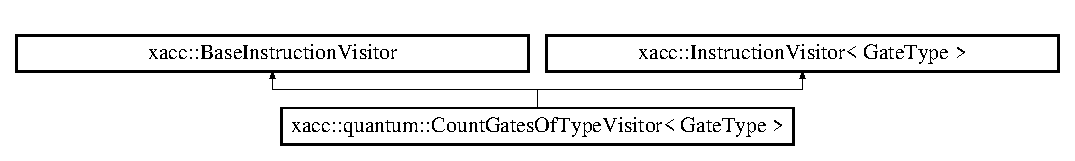
\includegraphics[height=12.000000cm]{a00039}
\end{center}
\end{figure}
\subsection*{Public Member Functions}
\begin{DoxyCompactItemize}
\item 
{\footnotesize template$<$typename HF , typename C\+NF , typename XF , typename YF , typename ZF , typename R\+XF , typename R\+YF , typename R\+ZF , typename MF , typename CF , typename C\+PF , typename S\+W\+A\+PF $>$ }\\{\bfseries Functional\+Gate\+Instruction\+Visitor} (HF h, C\+NF cn, XF x, YF y, ZF z, R\+XF rx, R\+YF ry, R\+ZF rz, MF m, CF c, C\+PF cp, S\+W\+A\+PF sw)\hypertarget{a00039_a4e3c27cd6b1acf063967b7b09a1eca09}{}\label{a00039_a4e3c27cd6b1acf063967b7b09a1eca09}

\item 
void {\bfseries visit} (\hyperlink{a00044}{Hadamard} \&h)\hypertarget{a00039_ac5245d34429dc112e7cd0e371108fcb5}{}\label{a00039_ac5245d34429dc112e7cd0e371108fcb5}

\item 
void {\bfseries visit} (\hyperlink{a00022}{C\+N\+OT} \&cn)\hypertarget{a00039_ad4eddafe8ca3906cd4aa5b98087a789a}{}\label{a00039_ad4eddafe8ca3906cd4aa5b98087a789a}

\item 
void {\bfseries visit} (\hyperlink{a00084}{X} \&x)\hypertarget{a00039_ac5d184daee7e755c9ede67b34bc2d091}{}\label{a00039_ac5d184daee7e755c9ede67b34bc2d091}

\item 
void {\bfseries visit} (\hyperlink{a00087}{Y} \&y)\hypertarget{a00039_a11dfa753a155346a45d7116a78c8f39f}{}\label{a00039_a11dfa753a155346a45d7116a78c8f39f}

\item 
void {\bfseries visit} (\hyperlink{a00088}{Z} \&z)\hypertarget{a00039_a4baf19da581fa9875739a227aba9cf60}{}\label{a00039_a4baf19da581fa9875739a227aba9cf60}

\item 
void {\bfseries visit} (\hyperlink{a00055}{Measure} \&m)\hypertarget{a00039_ad946faf8e2b6eff3e9e142907ec8e05a}{}\label{a00039_ad946faf8e2b6eff3e9e142907ec8e05a}

\item 
void {\bfseries visit} (\hyperlink{a00025}{Conditional\+Function} \&c)\hypertarget{a00039_a5cdb38902c241e7ae672a2631f1d61f3}{}\label{a00039_a5cdb38902c241e7ae672a2631f1d61f3}

\item 
void {\bfseries visit} (\hyperlink{a00073}{Rx} \&rx)\hypertarget{a00039_a6eb99e4b488773c750b7d9734ac1e885}{}\label{a00039_a6eb99e4b488773c750b7d9734ac1e885}

\item 
void {\bfseries visit} (\hyperlink{a00074}{Ry} \&ry)\hypertarget{a00039_aa22aad7b316386f5ef35672337c05ffc}{}\label{a00039_aa22aad7b316386f5ef35672337c05ffc}

\item 
void {\bfseries visit} (\hyperlink{a00027}{C\+Phase} \&cp)\hypertarget{a00039_a5475eece7afe380512a1a0215b92d302}{}\label{a00039_a5475eece7afe380512a1a0215b92d302}

\item 
void {\bfseries visit} (\hyperlink{a00075}{Rz} \&rz)\hypertarget{a00039_a8857ecf8f8f1b6143da8f31a722fe03e}{}\label{a00039_a8857ecf8f8f1b6143da8f31a722fe03e}

\item 
void {\bfseries visit} (\hyperlink{a00040}{Gate\+Function} \&f)\hypertarget{a00039_ad7d15225cf258fe59660ba828baff357}{}\label{a00039_ad7d15225cf258fe59660ba828baff357}

\item 
void {\bfseries visit} (\hyperlink{a00082}{Swap} \&s)\hypertarget{a00039_a30f46be43607813996c9cc090c1a5a16}{}\label{a00039_a30f46be43607813996c9cc090c1a5a16}

\end{DoxyCompactItemize}
\subsection*{Protected Attributes}
\begin{DoxyCompactItemize}
\item 
std\+::function$<$ void(\hyperlink{a00044}{Hadamard} \&)$>$ {\bfseries h\+Action}\hypertarget{a00039_a02f1401c9b0d1da801027f3bc0b5227e}{}\label{a00039_a02f1401c9b0d1da801027f3bc0b5227e}

\item 
std\+::function$<$ void(\hyperlink{a00022}{C\+N\+OT} \&)$>$ {\bfseries cnot\+Action}\hypertarget{a00039_a4d6bd8c2fd1af775ed08946942f60a0b}{}\label{a00039_a4d6bd8c2fd1af775ed08946942f60a0b}

\item 
std\+::function$<$ void(\hyperlink{a00084}{X} \&)$>$ {\bfseries x\+Action}\hypertarget{a00039_a9e0295434a2224b776609b057147a9af}{}\label{a00039_a9e0295434a2224b776609b057147a9af}

\item 
std\+::function$<$ void(\hyperlink{a00087}{Y} \&)$>$ {\bfseries y\+Action}\hypertarget{a00039_ae78f91a5cc9a7006f6bb1acee1c00501}{}\label{a00039_ae78f91a5cc9a7006f6bb1acee1c00501}

\item 
std\+::function$<$ void(\hyperlink{a00088}{Z} \&)$>$ {\bfseries z\+Action}\hypertarget{a00039_ae197f358e3d0777feb3656455e2ee672}{}\label{a00039_ae197f358e3d0777feb3656455e2ee672}

\item 
std\+::function$<$ void(\hyperlink{a00055}{Measure} \&)$>$ {\bfseries measure\+Action}\hypertarget{a00039_a239748abedd67c7b30cad12e545d1926}{}\label{a00039_a239748abedd67c7b30cad12e545d1926}

\item 
std\+::function$<$ void(\hyperlink{a00025}{Conditional\+Function} \&)$>$ {\bfseries cond\+Action}\hypertarget{a00039_a5c0595a70b1f7ae50f3e29a985e249e9}{}\label{a00039_a5c0595a70b1f7ae50f3e29a985e249e9}

\item 
std\+::function$<$ void(\hyperlink{a00073}{Rx} \&)$>$ {\bfseries rx\+Action}\hypertarget{a00039_ab79bb3eb3050d1c599061863bb2e219e}{}\label{a00039_ab79bb3eb3050d1c599061863bb2e219e}

\item 
std\+::function$<$ void(\hyperlink{a00074}{Ry} \&)$>$ {\bfseries ry\+Action}\hypertarget{a00039_a229b7d9aae52638c6eff04bd16bb9973}{}\label{a00039_a229b7d9aae52638c6eff04bd16bb9973}

\item 
std\+::function$<$ void(\hyperlink{a00075}{Rz} \&)$>$ {\bfseries rz\+Action}\hypertarget{a00039_a586ab5721150c67ad3ced46e2a236b44}{}\label{a00039_a586ab5721150c67ad3ced46e2a236b44}

\item 
std\+::function$<$ void(\hyperlink{a00027}{C\+Phase} \&)$>$ {\bfseries cp\+Action}\hypertarget{a00039_a5b88a0c9789e7b6d44527b2df6819ac5}{}\label{a00039_a5b88a0c9789e7b6d44527b2df6819ac5}

\item 
std\+::function$<$ void(\hyperlink{a00082}{Swap} \&)$>$ {\bfseries sw\+Action}\hypertarget{a00039_a5060cd4c2b1b259e32bda0e7ecc78e85}{}\label{a00039_a5060cd4c2b1b259e32bda0e7ecc78e85}

\end{DoxyCompactItemize}


The documentation for this class was generated from the following file\+:\begin{DoxyCompactItemize}
\item 
Functional\+Gate\+Instruction\+Visitor.\+hpp\end{DoxyCompactItemize}

\hypertarget{a00040}{}\section{Auto\+U\+TF$<$ Char\+Type $>$ Struct Template Reference}
\label{a00040}\index{Auto\+U\+T\+F$<$ Char\+Type $>$@{Auto\+U\+T\+F$<$ Char\+Type $>$}}


Dynamically select encoding according to stream\textquotesingle{}s runtime-\/specified U\+TF encoding type.  




{\ttfamily \#include $<$encodings.\+h$>$}

\subsection*{Public Types}
\begin{DoxyCompactItemize}
\item 
enum \{ {\bfseries support\+Unicode} = 1
 \}\hypertarget{a00040_aacfa2cfd9ad903c9c7110803c4037a7d}{}\label{a00040_aacfa2cfd9ad903c9c7110803c4037a7d}

\item 
typedef Char\+Type {\bfseries Ch}\hypertarget{a00040_a0609343de776df3bc31b4c980eb3cf1c}{}\label{a00040_a0609343de776df3bc31b4c980eb3cf1c}

\end{DoxyCompactItemize}
\subsection*{Static Public Member Functions}
\begin{DoxyCompactItemize}
\item 
{\footnotesize template$<$typename Output\+Stream $>$ }\\static R\+A\+P\+I\+D\+J\+S\+O\+N\+\_\+\+F\+O\+R\+C\+E\+I\+N\+L\+I\+NE void {\bfseries Encode} (Output\+Stream \&os, unsigned codepoint)\hypertarget{a00040_a414946115261f886e74dd42cb4b98781}{}\label{a00040_a414946115261f886e74dd42cb4b98781}

\item 
{\footnotesize template$<$typename Output\+Stream $>$ }\\static R\+A\+P\+I\+D\+J\+S\+O\+N\+\_\+\+F\+O\+R\+C\+E\+I\+N\+L\+I\+NE void {\bfseries Encode\+Unsafe} (Output\+Stream \&os, unsigned codepoint)\hypertarget{a00040_a05f5dcd1f153b61b763e44ed452de251}{}\label{a00040_a05f5dcd1f153b61b763e44ed452de251}

\item 
{\footnotesize template$<$typename Input\+Stream $>$ }\\static R\+A\+P\+I\+D\+J\+S\+O\+N\+\_\+\+F\+O\+R\+C\+E\+I\+N\+L\+I\+NE bool {\bfseries Decode} (Input\+Stream \&is, unsigned $\ast$codepoint)\hypertarget{a00040_aa5e3c1dc23dbb75f6442ff69500a35b0}{}\label{a00040_aa5e3c1dc23dbb75f6442ff69500a35b0}

\item 
{\footnotesize template$<$typename Input\+Stream , typename Output\+Stream $>$ }\\static R\+A\+P\+I\+D\+J\+S\+O\+N\+\_\+\+F\+O\+R\+C\+E\+I\+N\+L\+I\+NE bool {\bfseries Validate} (Input\+Stream \&is, Output\+Stream \&os)\hypertarget{a00040_a36dd6f226d6a07c12161e21c0aff20b1}{}\label{a00040_a36dd6f226d6a07c12161e21c0aff20b1}

\end{DoxyCompactItemize}


\subsection{Detailed Description}
\subsubsection*{template$<$typename Char\+Type$>$\\*
struct Auto\+U\+T\+F$<$ Char\+Type $>$}

Dynamically select encoding according to stream\textquotesingle{}s runtime-\/specified U\+TF encoding type. 

\begin{DoxyNote}{Note}
This class can be used with Auto\+U\+T\+F\+Inputt\+Stream and \hyperlink{a00042}{Auto\+U\+T\+F\+Output\+Stream}, which provides Get\+Type(). 
\end{DoxyNote}


The documentation for this struct was generated from the following file\+:\begin{DoxyCompactItemize}
\item 
encodings.\+h\end{DoxyCompactItemize}

\hypertarget{a00041}{}\section{xacc\+:\+:IR Class Reference}
\label{a00041}\index{xacc\+::\+IR@{xacc\+::\+IR}}


{\ttfamily \#include $<$I\+R.\+hpp$>$}

Inheritance diagram for xacc\+:\+:IR\+:\begin{figure}[H]
\begin{center}
\leavevmode
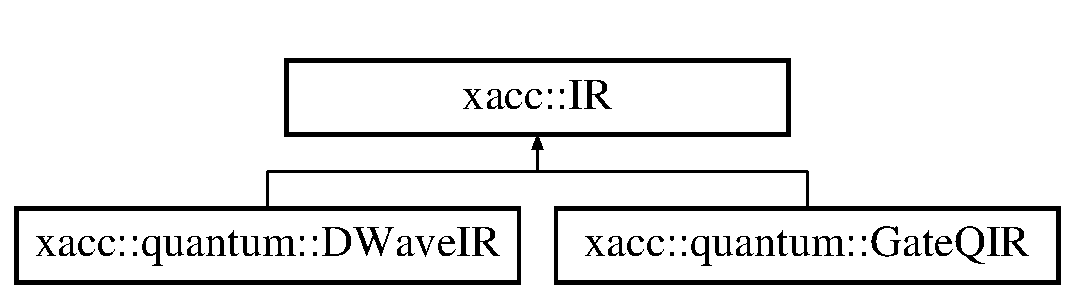
\includegraphics[height=2.000000cm]{a00041}
\end{center}
\end{figure}
\subsection*{Public Member Functions}
\begin{DoxyCompactItemize}
\item 
virtual std\+::string \hyperlink{a00041_a8356cdff1919b88eabeb84fd7450cdb6}{to\+Assembly\+String} (const std\+::string \&kernel\+Name, const std\+::string \&acc\+Buffer\+Var\+Name)=0
\item 
virtual void \hyperlink{a00041_a414b72224d88473ad6190bb88102a3ea}{persist} (std\+::ostream \&out\+Stream)=0
\item 
virtual void \hyperlink{a00041_a444c2e4dc0faac500fb70fa93997e9bc}{load} (std\+::istream \&in\+Stream)=0
\item 
virtual void \hyperlink{a00041_abbbf8e6993c518597de32cd05d49d737}{add\+Kernel} (std\+::shared\+\_\+ptr$<$ \hyperlink{a00030}{Function} $>$ kernel)=0
\item 
virtual bool \hyperlink{a00041_afc9ccf5126f3fed19c2e879133b2f6d8}{kernel\+Exists} (const std\+::string \&name)=0
\item 
virtual std\+::shared\+\_\+ptr$<$ \hyperlink{a00030}{Function} $>$ \hyperlink{a00041_a6f49b4ba4b3a15142b04873284885f0d}{get\+Kernel} (const std\+::string \&name)=0
\item 
virtual \hyperlink{a00041_a09a76d71092254acae07e19fa2f34921}{$\sim$\+IR} ()
\end{DoxyCompactItemize}


\subsection{Detailed Description}
The \hyperlink{a00041}{IR} interface is the base interface for derived accelerator-\/specific intermediate representations. At this level, an intermediate representation can be persisted to an assembly-\/like string, can be read in from file, and can be persisted to file. Since all X\+A\+CC intermediate representations operate on an \hyperlink{a00011}{Accelerator} Buffer, the \hyperlink{a00041}{IR} interface also provides a setter for such a buffer. 

\subsection{Constructor \& Destructor Documentation}
\index{xacc\+::\+IR@{xacc\+::\+IR}!````~IR@{$\sim$\+IR}}
\index{````~IR@{$\sim$\+IR}!xacc\+::\+IR@{xacc\+::\+IR}}
\subsubsection[{\texorpdfstring{$\sim$\+I\+R()}{~IR()}}]{\setlength{\rightskip}{0pt plus 5cm}virtual xacc\+::\+I\+R\+::$\sim$\+IR (
\begin{DoxyParamCaption}
{}
\end{DoxyParamCaption}
)\hspace{0.3cm}{\ttfamily [inline]}, {\ttfamily [virtual]}}\hypertarget{a00041_a09a76d71092254acae07e19fa2f34921}{}\label{a00041_a09a76d71092254acae07e19fa2f34921}
The destructor 

\subsection{Member Function Documentation}
\index{xacc\+::\+IR@{xacc\+::\+IR}!add\+Kernel@{add\+Kernel}}
\index{add\+Kernel@{add\+Kernel}!xacc\+::\+IR@{xacc\+::\+IR}}
\subsubsection[{\texorpdfstring{add\+Kernel(std\+::shared\+\_\+ptr$<$ Function $>$ kernel)=0}{addKernel(std::shared\_ptr< Function > kernel)=0}}]{\setlength{\rightskip}{0pt plus 5cm}virtual void xacc\+::\+I\+R\+::add\+Kernel (
\begin{DoxyParamCaption}
\item[{std\+::shared\+\_\+ptr$<$ {\bf Function} $>$}]{kernel}
\end{DoxyParamCaption}
)\hspace{0.3cm}{\ttfamily [pure virtual]}}\hypertarget{a00041_abbbf8e6993c518597de32cd05d49d737}{}\label{a00041_abbbf8e6993c518597de32cd05d49d737}
Add a new kernel to this \hyperlink{a00041}{IR} instance.


\begin{DoxyParams}{Parameters}
{\em kernel} & The \hyperlink{a00030}{Function} instance to add as a new kernel \\
\hline
\end{DoxyParams}


Implemented in \hyperlink{a00034_aa6ed2cf2cbcfec8105c327a4fa95346f}{xacc\+::quantum\+::\+Gate\+Q\+IR}, and \hyperlink{a00025_a7e1ddff2771233dc45f60a6b7e15ef63}{xacc\+::quantum\+::\+D\+Wave\+IR}.

\index{xacc\+::\+IR@{xacc\+::\+IR}!get\+Kernel@{get\+Kernel}}
\index{get\+Kernel@{get\+Kernel}!xacc\+::\+IR@{xacc\+::\+IR}}
\subsubsection[{\texorpdfstring{get\+Kernel(const std\+::string \&name)=0}{getKernel(const std::string \&name)=0}}]{\setlength{\rightskip}{0pt plus 5cm}virtual std\+::shared\+\_\+ptr$<${\bf Function}$>$ xacc\+::\+I\+R\+::get\+Kernel (
\begin{DoxyParamCaption}
\item[{const std\+::string \&}]{name}
\end{DoxyParamCaption}
)\hspace{0.3cm}{\ttfamily [pure virtual]}}\hypertarget{a00041_a6f49b4ba4b3a15142b04873284885f0d}{}\label{a00041_a6f49b4ba4b3a15142b04873284885f0d}
Return the kernel with the given name.


\begin{DoxyParams}{Parameters}
{\em name} & The name of the kernel to return. \\
\hline
\end{DoxyParams}
\begin{DoxyReturn}{Returns}
kernel The kernel with given name. 
\end{DoxyReturn}


Implemented in \hyperlink{a00034_a194758b6edcc3ae0c7fe8004f9bfe690}{xacc\+::quantum\+::\+Gate\+Q\+IR}, and \hyperlink{a00025_ac4295dfef98c94d7154a4fd39a6e5d1c}{xacc\+::quantum\+::\+D\+Wave\+IR}.

\index{xacc\+::\+IR@{xacc\+::\+IR}!kernel\+Exists@{kernel\+Exists}}
\index{kernel\+Exists@{kernel\+Exists}!xacc\+::\+IR@{xacc\+::\+IR}}
\subsubsection[{\texorpdfstring{kernel\+Exists(const std\+::string \&name)=0}{kernelExists(const std::string \&name)=0}}]{\setlength{\rightskip}{0pt plus 5cm}virtual bool xacc\+::\+I\+R\+::kernel\+Exists (
\begin{DoxyParamCaption}
\item[{const std\+::string \&}]{name}
\end{DoxyParamCaption}
)\hspace{0.3cm}{\ttfamily [pure virtual]}}\hypertarget{a00041_afc9ccf5126f3fed19c2e879133b2f6d8}{}\label{a00041_afc9ccf5126f3fed19c2e879133b2f6d8}
Return true if the kernel with given name exists in this \hyperlink{a00041}{IR}.


\begin{DoxyParams}{Parameters}
{\em name} & The name of the kernel to return. \\
\hline
\end{DoxyParams}
\begin{DoxyReturn}{Returns}
exists True if kernel exists. 
\end{DoxyReturn}


Implemented in \hyperlink{a00034_a692f95099caa7c024110a3f035941dca}{xacc\+::quantum\+::\+Gate\+Q\+IR}, and \hyperlink{a00025_ace9b8c6f4f29e32c8482fec4eacb637a}{xacc\+::quantum\+::\+D\+Wave\+IR}.

\index{xacc\+::\+IR@{xacc\+::\+IR}!load@{load}}
\index{load@{load}!xacc\+::\+IR@{xacc\+::\+IR}}
\subsubsection[{\texorpdfstring{load(std\+::istream \&in\+Stream)=0}{load(std::istream \&inStream)=0}}]{\setlength{\rightskip}{0pt plus 5cm}virtual void xacc\+::\+I\+R\+::load (
\begin{DoxyParamCaption}
\item[{std\+::istream \&}]{in\+Stream}
\end{DoxyParamCaption}
)\hspace{0.3cm}{\ttfamily [pure virtual]}}\hypertarget{a00041_a444c2e4dc0faac500fb70fa93997e9bc}{}\label{a00041_a444c2e4dc0faac500fb70fa93997e9bc}
Create this \hyperlink{a00041}{IR} instance from the given input stream.


\begin{DoxyParams}{Parameters}
{\em in\+Stream} & The input stream to read from. \\
\hline
\end{DoxyParams}


Implemented in \hyperlink{a00034_a07f26eeb362ac480d20da6cdc8c8fb39}{xacc\+::quantum\+::\+Gate\+Q\+IR}, and \hyperlink{a00025_a94d814172ec30c7ed32e6ab52bc2a41a}{xacc\+::quantum\+::\+D\+Wave\+IR}.

\index{xacc\+::\+IR@{xacc\+::\+IR}!persist@{persist}}
\index{persist@{persist}!xacc\+::\+IR@{xacc\+::\+IR}}
\subsubsection[{\texorpdfstring{persist(std\+::ostream \&out\+Stream)=0}{persist(std::ostream \&outStream)=0}}]{\setlength{\rightskip}{0pt plus 5cm}virtual void xacc\+::\+I\+R\+::persist (
\begin{DoxyParamCaption}
\item[{std\+::ostream \&}]{out\+Stream}
\end{DoxyParamCaption}
)\hspace{0.3cm}{\ttfamily [pure virtual]}}\hypertarget{a00041_a414b72224d88473ad6190bb88102a3ea}{}\label{a00041_a414b72224d88473ad6190bb88102a3ea}
Persist this \hyperlink{a00041}{IR} instance to the given output stream.


\begin{DoxyParams}{Parameters}
{\em out\+Stream} & The output stream to persist to. \\
\hline
\end{DoxyParams}


Implemented in \hyperlink{a00034_a40e1d07e4dfd3794ef53fca3cdbdca61}{xacc\+::quantum\+::\+Gate\+Q\+IR}, and \hyperlink{a00025_adac268c6fa2234902efeb9b3c07c0ac2}{xacc\+::quantum\+::\+D\+Wave\+IR}.

\index{xacc\+::\+IR@{xacc\+::\+IR}!to\+Assembly\+String@{to\+Assembly\+String}}
\index{to\+Assembly\+String@{to\+Assembly\+String}!xacc\+::\+IR@{xacc\+::\+IR}}
\subsubsection[{\texorpdfstring{to\+Assembly\+String(const std\+::string \&kernel\+Name, const std\+::string \&acc\+Buffer\+Var\+Name)=0}{toAssemblyString(const std::string \&kernelName, const std::string \&accBufferVarName)=0}}]{\setlength{\rightskip}{0pt plus 5cm}virtual std\+::string xacc\+::\+I\+R\+::to\+Assembly\+String (
\begin{DoxyParamCaption}
\item[{const std\+::string \&}]{kernel\+Name, }
\item[{const std\+::string \&}]{acc\+Buffer\+Var\+Name}
\end{DoxyParamCaption}
)\hspace{0.3cm}{\ttfamily [pure virtual]}}\hypertarget{a00041_a8356cdff1919b88eabeb84fd7450cdb6}{}\label{a00041_a8356cdff1919b88eabeb84fd7450cdb6}
Return a assembly-\/like string representation of this intermediate representation


\begin{DoxyParams}{Parameters}
{\em kernel\+Name} & The name of hte kernel to persist to string \\
\hline
{\em acc\+Buffer\+Var\+Name} & The name of the \hyperlink{a00013}{Accelerator\+Buffer} \\
\hline
\end{DoxyParams}
\begin{DoxyReturn}{Returns}

\end{DoxyReturn}


Implemented in \hyperlink{a00034_a7153f7e9f516d43af3d5d4f95d60bd86}{xacc\+::quantum\+::\+Gate\+Q\+IR}, and \hyperlink{a00025_ac19ad098d5bbfe769809c10e26ebebc6}{xacc\+::quantum\+::\+D\+Wave\+IR}.



The documentation for this class was generated from the following file\+:\begin{DoxyCompactItemize}
\item 
I\+R.\+hpp\end{DoxyCompactItemize}

\hypertarget{a00042}{}\section{xacc\+:\+:I\+R\+Transformation Class Reference}
\label{a00042}\index{xacc\+::\+I\+R\+Transformation@{xacc\+::\+I\+R\+Transformation}}
\subsection*{Public Member Functions}
\begin{DoxyCompactItemize}
\item 
virtual void {\bfseries transform} (\hyperlink{a00041}{IR} \&ir)=0\hypertarget{a00042_accc69cba97f39aa3e51f81fec3ccf258}{}\label{a00042_accc69cba97f39aa3e51f81fec3ccf258}

\end{DoxyCompactItemize}


The documentation for this class was generated from the following file\+:\begin{DoxyCompactItemize}
\item 
I\+R\+Transformation.\+hpp\end{DoxyCompactItemize}

\hypertarget{a00043}{}\section{xacc\+:\+:is\+\_\+valid\+\_\+vertex$<$ T, typename $>$ Struct Template Reference}
\label{a00043}\index{xacc\+::is\+\_\+valid\+\_\+vertex$<$ T, typename $>$@{xacc\+::is\+\_\+valid\+\_\+vertex$<$ T, typename $>$}}


{\ttfamily \#include $<$Graph.\+hpp$>$}

Inheritance diagram for xacc\+:\+:is\+\_\+valid\+\_\+vertex$<$ T, typename $>$\+:\begin{figure}[H]
\begin{center}
\leavevmode
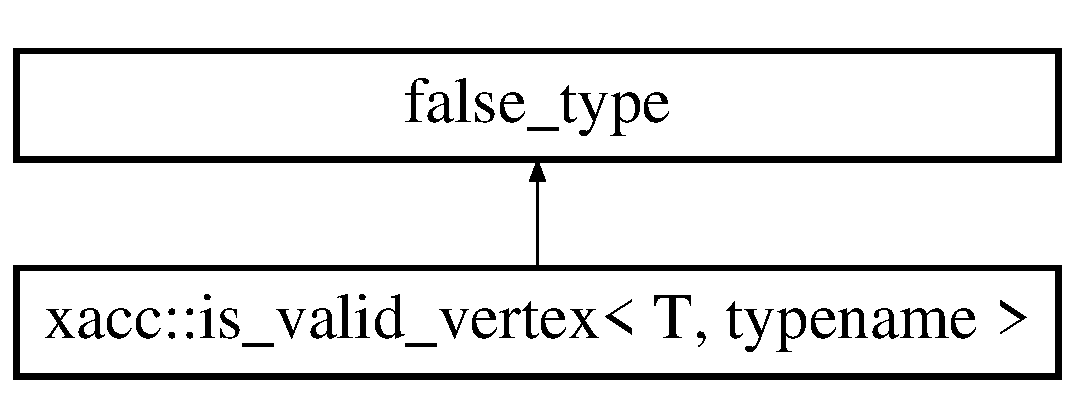
\includegraphics[height=2.000000cm]{a00043}
\end{center}
\end{figure}


\subsection{Detailed Description}
\subsubsection*{template$<$typename T, typename = void$>$\\*
struct xacc\+::is\+\_\+valid\+\_\+vertex$<$ T, typename $>$}

Utility structs to help determine if we have been given valid Vertices. 

The documentation for this struct was generated from the following file\+:\begin{DoxyCompactItemize}
\item 
Graph.\+hpp\end{DoxyCompactItemize}

\hypertarget{a00044}{}\section{xacc\+:\+:quantum\+:\+:D\+W\+IR Class Reference}
\label{a00044}\index{xacc\+::quantum\+::\+D\+W\+IR@{xacc\+::quantum\+::\+D\+W\+IR}}
Inheritance diagram for xacc\+:\+:quantum\+:\+:D\+W\+IR\+:\begin{figure}[H]
\begin{center}
\leavevmode
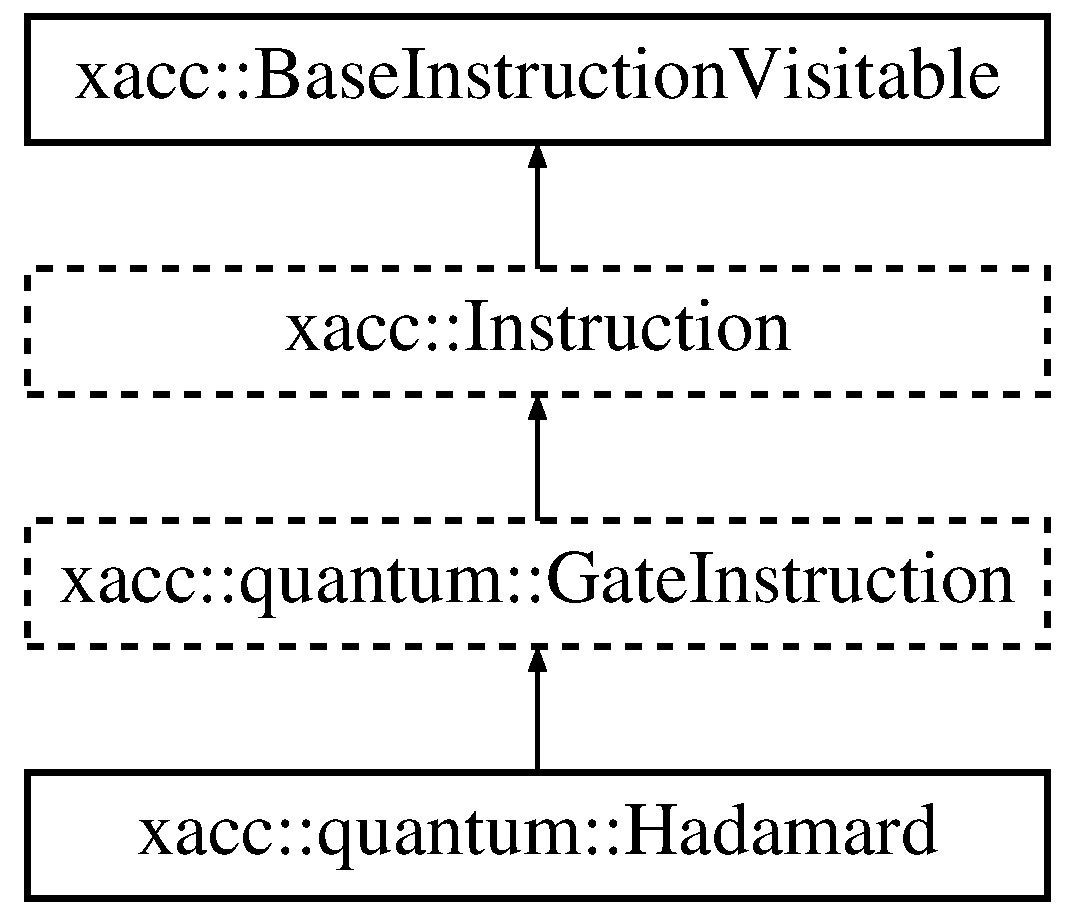
\includegraphics[height=2.000000cm]{a00044}
\end{center}
\end{figure}
\subsection*{Public Member Functions}
\begin{DoxyCompactItemize}
\item 
virtual std\+::string \hyperlink{a00044_a880cb60197577ea31115331e3a030e3e}{to\+Assembly\+String} (const std\+::string \&kernel\+Name, const std\+::string \&acc\+Buffer\+Var\+Name)
\item 
virtual void \hyperlink{a00044_abcbfd0a4cf697843391c65cbd9a82080}{persist} (std\+::ostream \&out\+Stream)
\item 
virtual void \hyperlink{a00044_a8b388d719d565bb902c979807d3d0d47}{load} (std\+::istream \&in\+Stream)
\item 
virtual void \hyperlink{a00044_af1bef18e1e9568d1313b03149aab8c1b}{add\+Kernel} (std\+::shared\+\_\+ptr$<$ \hyperlink{a00059}{Function} $>$ kernel)
\item 
virtual bool \hyperlink{a00044_ab5e8861d3bc0845bb015af6208f5f396}{kernel\+Exists} (const std\+::string \&name)
\item 
virtual std\+::shared\+\_\+ptr$<$ \hyperlink{a00059}{Function} $>$ \hyperlink{a00044_a38d8bdd24250749bc38ad31f8512fcfc}{get\+Kernel} (const std\+::string \&name)
\item 
virtual std\+::vector$<$ std\+::shared\+\_\+ptr$<$ \hyperlink{a00059}{Function} $>$ $>$ \hyperlink{a00044_a66e22c5dc95ec46045476864012ad08f}{get\+Kernels} ()
\end{DoxyCompactItemize}
\subsection*{Protected Attributes}
\begin{DoxyCompactItemize}
\item 
std\+::vector$<$ std\+::shared\+\_\+ptr$<$ \hyperlink{a00059}{Function} $>$ $>$ \hyperlink{a00044_abcb04ec3a152c3f22e5a757a9aecabf2}{kernels}
\end{DoxyCompactItemize}


\subsection{Member Function Documentation}
\index{xacc\+::quantum\+::\+D\+W\+IR@{xacc\+::quantum\+::\+D\+W\+IR}!add\+Kernel@{add\+Kernel}}
\index{add\+Kernel@{add\+Kernel}!xacc\+::quantum\+::\+D\+W\+IR@{xacc\+::quantum\+::\+D\+W\+IR}}
\subsubsection[{\texorpdfstring{add\+Kernel(std\+::shared\+\_\+ptr$<$ Function $>$ kernel)}{addKernel(std::shared\_ptr< Function > kernel)}}]{\setlength{\rightskip}{0pt plus 5cm}virtual void xacc\+::quantum\+::\+D\+W\+I\+R\+::add\+Kernel (
\begin{DoxyParamCaption}
\item[{std\+::shared\+\_\+ptr$<$ {\bf Function} $>$}]{kernel}
\end{DoxyParamCaption}
)\hspace{0.3cm}{\ttfamily [inline]}, {\ttfamily [virtual]}}\hypertarget{a00044_af1bef18e1e9568d1313b03149aab8c1b}{}\label{a00044_af1bef18e1e9568d1313b03149aab8c1b}
Add a new kernel to this \hyperlink{a00077}{IR} instance.


\begin{DoxyParams}{Parameters}
{\em kernel} & The \hyperlink{a00059}{Function} instance to add as a new kernel \\
\hline
\end{DoxyParams}


Implements \hyperlink{a00077_abbbf8e6993c518597de32cd05d49d737}{xacc\+::\+IR}.

\index{xacc\+::quantum\+::\+D\+W\+IR@{xacc\+::quantum\+::\+D\+W\+IR}!get\+Kernel@{get\+Kernel}}
\index{get\+Kernel@{get\+Kernel}!xacc\+::quantum\+::\+D\+W\+IR@{xacc\+::quantum\+::\+D\+W\+IR}}
\subsubsection[{\texorpdfstring{get\+Kernel(const std\+::string \&name)}{getKernel(const std::string \&name)}}]{\setlength{\rightskip}{0pt plus 5cm}virtual std\+::shared\+\_\+ptr$<${\bf Function}$>$ xacc\+::quantum\+::\+D\+W\+I\+R\+::get\+Kernel (
\begin{DoxyParamCaption}
\item[{const std\+::string \&}]{name}
\end{DoxyParamCaption}
)\hspace{0.3cm}{\ttfamily [inline]}, {\ttfamily [virtual]}}\hypertarget{a00044_a38d8bdd24250749bc38ad31f8512fcfc}{}\label{a00044_a38d8bdd24250749bc38ad31f8512fcfc}
Return the kernel with the given name.


\begin{DoxyParams}{Parameters}
{\em name} & The name of the kernel to return. \\
\hline
\end{DoxyParams}
\begin{DoxyReturn}{Returns}
kernel The kernel with given name. 
\end{DoxyReturn}


Implements \hyperlink{a00077_a6f49b4ba4b3a15142b04873284885f0d}{xacc\+::\+IR}.

\index{xacc\+::quantum\+::\+D\+W\+IR@{xacc\+::quantum\+::\+D\+W\+IR}!get\+Kernels@{get\+Kernels}}
\index{get\+Kernels@{get\+Kernels}!xacc\+::quantum\+::\+D\+W\+IR@{xacc\+::quantum\+::\+D\+W\+IR}}
\subsubsection[{\texorpdfstring{get\+Kernels()}{getKernels()}}]{\setlength{\rightskip}{0pt plus 5cm}virtual std\+::vector$<$std\+::shared\+\_\+ptr$<${\bf Function}$>$ $>$ xacc\+::quantum\+::\+D\+W\+I\+R\+::get\+Kernels (
\begin{DoxyParamCaption}
{}
\end{DoxyParamCaption}
)\hspace{0.3cm}{\ttfamily [inline]}, {\ttfamily [virtual]}}\hypertarget{a00044_a66e22c5dc95ec46045476864012ad08f}{}\label{a00044_a66e22c5dc95ec46045476864012ad08f}
Return all of this \hyperlink{a00077}{IR} instance\textquotesingle{}s kernels.

\begin{DoxyReturn}{Returns}
kernels The kernels this \hyperlink{a00077}{IR} contains. 
\end{DoxyReturn}


Implements \hyperlink{a00077_a88c50bfc5b279145360ddc0c3a703b9b}{xacc\+::\+IR}.

\index{xacc\+::quantum\+::\+D\+W\+IR@{xacc\+::quantum\+::\+D\+W\+IR}!kernel\+Exists@{kernel\+Exists}}
\index{kernel\+Exists@{kernel\+Exists}!xacc\+::quantum\+::\+D\+W\+IR@{xacc\+::quantum\+::\+D\+W\+IR}}
\subsubsection[{\texorpdfstring{kernel\+Exists(const std\+::string \&name)}{kernelExists(const std::string \&name)}}]{\setlength{\rightskip}{0pt plus 5cm}virtual bool xacc\+::quantum\+::\+D\+W\+I\+R\+::kernel\+Exists (
\begin{DoxyParamCaption}
\item[{const std\+::string \&}]{name}
\end{DoxyParamCaption}
)\hspace{0.3cm}{\ttfamily [inline]}, {\ttfamily [virtual]}}\hypertarget{a00044_ab5e8861d3bc0845bb015af6208f5f396}{}\label{a00044_ab5e8861d3bc0845bb015af6208f5f396}
Return true if the kernel with given name exists in this \hyperlink{a00077}{IR}.


\begin{DoxyParams}{Parameters}
{\em name} & The name of the kernel to return. \\
\hline
\end{DoxyParams}
\begin{DoxyReturn}{Returns}
exists True if kernel exists. 
\end{DoxyReturn}


Implements \hyperlink{a00077_afc9ccf5126f3fed19c2e879133b2f6d8}{xacc\+::\+IR}.

\index{xacc\+::quantum\+::\+D\+W\+IR@{xacc\+::quantum\+::\+D\+W\+IR}!load@{load}}
\index{load@{load}!xacc\+::quantum\+::\+D\+W\+IR@{xacc\+::quantum\+::\+D\+W\+IR}}
\subsubsection[{\texorpdfstring{load(std\+::istream \&in\+Stream)}{load(std::istream \&inStream)}}]{\setlength{\rightskip}{0pt plus 5cm}virtual void xacc\+::quantum\+::\+D\+W\+I\+R\+::load (
\begin{DoxyParamCaption}
\item[{std\+::istream \&}]{in\+Stream}
\end{DoxyParamCaption}
)\hspace{0.3cm}{\ttfamily [inline]}, {\ttfamily [virtual]}}\hypertarget{a00044_a8b388d719d565bb902c979807d3d0d47}{}\label{a00044_a8b388d719d565bb902c979807d3d0d47}
Create this \hyperlink{a00077}{IR} instance from the given input stream.


\begin{DoxyParams}{Parameters}
{\em in\+Stream} & \\
\hline
\end{DoxyParams}


Implements \hyperlink{a00077_a444c2e4dc0faac500fb70fa93997e9bc}{xacc\+::\+IR}.

\index{xacc\+::quantum\+::\+D\+W\+IR@{xacc\+::quantum\+::\+D\+W\+IR}!persist@{persist}}
\index{persist@{persist}!xacc\+::quantum\+::\+D\+W\+IR@{xacc\+::quantum\+::\+D\+W\+IR}}
\subsubsection[{\texorpdfstring{persist(std\+::ostream \&out\+Stream)}{persist(std::ostream \&outStream)}}]{\setlength{\rightskip}{0pt plus 5cm}virtual void xacc\+::quantum\+::\+D\+W\+I\+R\+::persist (
\begin{DoxyParamCaption}
\item[{std\+::ostream \&}]{out\+Stream}
\end{DoxyParamCaption}
)\hspace{0.3cm}{\ttfamily [inline]}, {\ttfamily [virtual]}}\hypertarget{a00044_abcbfd0a4cf697843391c65cbd9a82080}{}\label{a00044_abcbfd0a4cf697843391c65cbd9a82080}
Persist this \hyperlink{a00077}{IR} instance to the given output stream.


\begin{DoxyParams}{Parameters}
{\em out\+Stream} & \\
\hline
\end{DoxyParams}


Implements \hyperlink{a00077_a414b72224d88473ad6190bb88102a3ea}{xacc\+::\+IR}.

\index{xacc\+::quantum\+::\+D\+W\+IR@{xacc\+::quantum\+::\+D\+W\+IR}!to\+Assembly\+String@{to\+Assembly\+String}}
\index{to\+Assembly\+String@{to\+Assembly\+String}!xacc\+::quantum\+::\+D\+W\+IR@{xacc\+::quantum\+::\+D\+W\+IR}}
\subsubsection[{\texorpdfstring{to\+Assembly\+String(const std\+::string \&kernel\+Name, const std\+::string \&acc\+Buffer\+Var\+Name)}{toAssemblyString(const std::string \&kernelName, const std::string \&accBufferVarName)}}]{\setlength{\rightskip}{0pt plus 5cm}virtual std\+::string xacc\+::quantum\+::\+D\+W\+I\+R\+::to\+Assembly\+String (
\begin{DoxyParamCaption}
\item[{const std\+::string \&}]{kernel\+Name, }
\item[{const std\+::string \&}]{acc\+Buffer\+Var\+Name}
\end{DoxyParamCaption}
)\hspace{0.3cm}{\ttfamily [inline]}, {\ttfamily [virtual]}}\hypertarget{a00044_a880cb60197577ea31115331e3a030e3e}{}\label{a00044_a880cb60197577ea31115331e3a030e3e}
Return a assembly-\/like string representation of this intermediate representation \begin{DoxyReturn}{Returns}

\end{DoxyReturn}


Implements \hyperlink{a00077_a8356cdff1919b88eabeb84fd7450cdb6}{xacc\+::\+IR}.



\subsection{Member Data Documentation}
\index{xacc\+::quantum\+::\+D\+W\+IR@{xacc\+::quantum\+::\+D\+W\+IR}!kernels@{kernels}}
\index{kernels@{kernels}!xacc\+::quantum\+::\+D\+W\+IR@{xacc\+::quantum\+::\+D\+W\+IR}}
\subsubsection[{\texorpdfstring{kernels}{kernels}}]{\setlength{\rightskip}{0pt plus 5cm}std\+::vector$<$std\+::shared\+\_\+ptr$<${\bf Function}$>$ $>$ xacc\+::quantum\+::\+D\+W\+I\+R\+::kernels\hspace{0.3cm}{\ttfamily [protected]}}\hypertarget{a00044_abcb04ec3a152c3f22e5a757a9aecabf2}{}\label{a00044_abcb04ec3a152c3f22e5a757a9aecabf2}
Reference to this Q\+IR\textquotesingle{}s list of quantum functions 

The documentation for this class was generated from the following file\+:\begin{DoxyCompactItemize}
\item 
D\+W\+I\+R.\+hpp\end{DoxyCompactItemize}

\hypertarget{a00045}{}\section{xacc\+:\+:quantum\+:\+:D\+W\+Kernel Class Reference}
\label{a00045}\index{xacc\+::quantum\+::\+D\+W\+Kernel@{xacc\+::quantum\+::\+D\+W\+Kernel}}


{\ttfamily \#include $<$D\+W\+Kernel.\+hpp$>$}

Inheritance diagram for xacc\+:\+:quantum\+:\+:D\+W\+Kernel\+:\begin{figure}[H]
\begin{center}
\leavevmode
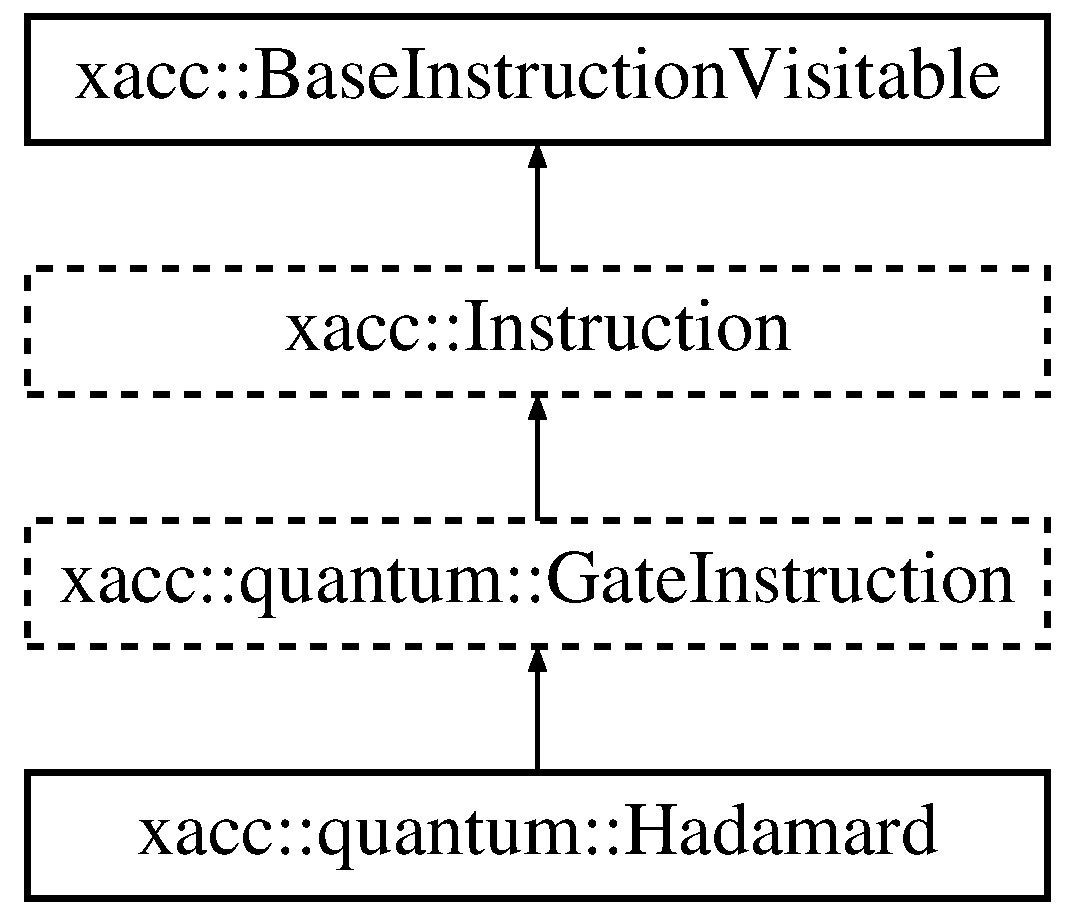
\includegraphics[height=4.000000cm]{a00045}
\end{center}
\end{figure}
\subsection*{Public Member Functions}
\begin{DoxyCompactItemize}
\item 
\hyperlink{a00045_a76a4dfadb973abbc93d1afefc6839ad8}{D\+W\+Kernel} (std\+::string kernel\+Name)
\item 
virtual const int \hyperlink{a00045_a79aecc7419a20b8779372ef36fc24806}{n\+Instructions} ()
\item 
virtual Inst\+Ptr \hyperlink{a00045_a00f23cd2e15ea6b9d00d4f3dbe1540f8}{get\+Instruction} (const int idx)
\item 
virtual std\+::list$<$ Inst\+Ptr $>$ \hyperlink{a00045_abbb8f2b1c78623c377524e45d581d018}{get\+Instructions} ()
\item 
virtual void \hyperlink{a00045_af2bcfd679e6cb89194f3f0bff8622b99}{remove\+Instruction} (const int idx)
\item 
virtual void \hyperlink{a00045_a4c3043d6971999c3a09e797fc55deb6c}{add\+Instruction} (Inst\+Ptr instruction)
\item 
virtual void \hyperlink{a00045_a75eb3560d2f81c9a5ae1cf765deb0e83}{replace\+Instruction} (const int idx, Inst\+Ptr replacing\+Inst)
\item 
virtual void \hyperlink{a00045_a1627af0141f70fc4a3cd500a13fb31b8}{insert\+Instruction} (const int idx, Inst\+Ptr new\+Inst)
\item 
virtual const std\+::string \hyperlink{a00045_a7f0c4d3c73029566561cf56a474bcbbd}{get\+Name} ()
\item 
virtual const std\+::vector$<$ int $>$ \hyperlink{a00045_adae68964db6acd8b4c2267c270a8ec58}{bits} ()
\item 
virtual const std\+::string \hyperlink{a00045_adbc3fdd080ebba20bc620b8832979f16}{to\+String} (const std\+::string \&buffer\+Var\+Name)
\item 
std\+::vector$<$ double $>$ {\bfseries get\+All\+Biases} ()\hypertarget{a00045_a9ee05b3d7689bbf837bdb7737f9745f4}{}\label{a00045_a9ee05b3d7689bbf837bdb7737f9745f4}

\item 
std\+::vector$<$ double $>$ {\bfseries get\+All\+Couplers} ()\hypertarget{a00045_a7df03ecec9c1821433daa3aa092cbd4d}{}\label{a00045_a7df03ecec9c1821433daa3aa092cbd4d}

\item 
virtual Instruction\+Parameter \hyperlink{a00045_a81711b7db284aba35d6952e4d1d15d41}{get\+Parameter} (const int idx)
\item 
virtual void \hyperlink{a00045_adf89cdd1f54e183c4cff36b338b2be8d}{set\+Parameter} (const int idx, Instruction\+Parameter \&p)
\item 
virtual std\+::vector$<$ Instruction\+Parameter $>$ \hyperlink{a00045_a829462cff34e2257da06afd8a2051a8e}{get\+Parameters} ()
\item 
virtual bool \hyperlink{a00045_a8957ea368244ed4a4ebd85f6bfecb785}{is\+Parameterized} ()
\item 
virtual const int \hyperlink{a00045_a029429948329b94c1d89f32cf5c486d4}{n\+Parameters} ()
\item 
virtual void \hyperlink{a00045_a09ffac417d4ecbbd82d7a680ad8dfcce}{evaluate\+Variable\+Parameters} (std\+::vector$<$ Instruction\+Parameter $>$ parameters)
\end{DoxyCompactItemize}
\subsection*{Protected Attributes}
\begin{DoxyCompactItemize}
\item 
std\+::list$<$ Inst\+Ptr $>$ {\bfseries instructions}\hypertarget{a00045_a38e434be6ef46a1ff43744632ae59ea8}{}\label{a00045_a38e434be6ef46a1ff43744632ae59ea8}

\item 
std\+::string {\bfseries name}\hypertarget{a00045_a0df03f85cc3b8a4cd1a7fc839d4d303c}{}\label{a00045_a0df03f85cc3b8a4cd1a7fc839d4d303c}

\end{DoxyCompactItemize}
\subsection*{Additional Inherited Members}


\subsection{Detailed Description}
The \hyperlink{a00045}{D\+W\+Kernel} is an X\+A\+CC \hyperlink{a00059}{Function} that contains \hyperlink{a00046}{D\+W\+Q\+MI} Instructions. 

\subsection{Constructor \& Destructor Documentation}
\index{xacc\+::quantum\+::\+D\+W\+Kernel@{xacc\+::quantum\+::\+D\+W\+Kernel}!D\+W\+Kernel@{D\+W\+Kernel}}
\index{D\+W\+Kernel@{D\+W\+Kernel}!xacc\+::quantum\+::\+D\+W\+Kernel@{xacc\+::quantum\+::\+D\+W\+Kernel}}
\subsubsection[{\texorpdfstring{D\+W\+Kernel(std\+::string kernel\+Name)}{DWKernel(std::string kernelName)}}]{\setlength{\rightskip}{0pt plus 5cm}xacc\+::quantum\+::\+D\+W\+Kernel\+::\+D\+W\+Kernel (
\begin{DoxyParamCaption}
\item[{std\+::string}]{kernel\+Name}
\end{DoxyParamCaption}
)\hspace{0.3cm}{\ttfamily [inline]}}\hypertarget{a00045_a76a4dfadb973abbc93d1afefc6839ad8}{}\label{a00045_a76a4dfadb973abbc93d1afefc6839ad8}
The constructor, takes the function unique id and its name.


\begin{DoxyParams}{Parameters}
{\em id} & \\
\hline
{\em name} & \\
\hline
\end{DoxyParams}


\subsection{Member Function Documentation}
\index{xacc\+::quantum\+::\+D\+W\+Kernel@{xacc\+::quantum\+::\+D\+W\+Kernel}!add\+Instruction@{add\+Instruction}}
\index{add\+Instruction@{add\+Instruction}!xacc\+::quantum\+::\+D\+W\+Kernel@{xacc\+::quantum\+::\+D\+W\+Kernel}}
\subsubsection[{\texorpdfstring{add\+Instruction(\+Inst\+Ptr instruction)}{addInstruction(InstPtr instruction)}}]{\setlength{\rightskip}{0pt plus 5cm}virtual void xacc\+::quantum\+::\+D\+W\+Kernel\+::add\+Instruction (
\begin{DoxyParamCaption}
\item[{Inst\+Ptr}]{instruction}
\end{DoxyParamCaption}
)\hspace{0.3cm}{\ttfamily [inline]}, {\ttfamily [virtual]}}\hypertarget{a00045_a4c3043d6971999c3a09e797fc55deb6c}{}\label{a00045_a4c3043d6971999c3a09e797fc55deb6c}
Add an instruction to this quantum intermediate representation.


\begin{DoxyParams}{Parameters}
{\em instruction} & \\
\hline
\end{DoxyParams}


Implements \hyperlink{a00059_aa8c9ec2d08be75c69399d4254b0216f5}{xacc\+::\+Function}.

\index{xacc\+::quantum\+::\+D\+W\+Kernel@{xacc\+::quantum\+::\+D\+W\+Kernel}!bits@{bits}}
\index{bits@{bits}!xacc\+::quantum\+::\+D\+W\+Kernel@{xacc\+::quantum\+::\+D\+W\+Kernel}}
\subsubsection[{\texorpdfstring{bits()}{bits()}}]{\setlength{\rightskip}{0pt plus 5cm}virtual const std\+::vector$<$int$>$ xacc\+::quantum\+::\+D\+W\+Kernel\+::bits (
\begin{DoxyParamCaption}
{}
\end{DoxyParamCaption}
)\hspace{0.3cm}{\ttfamily [inline]}, {\ttfamily [virtual]}}\hypertarget{a00045_adae68964db6acd8b4c2267c270a8ec58}{}\label{a00045_adae68964db6acd8b4c2267c270a8ec58}
Return the qubits this function acts on. \begin{DoxyReturn}{Returns}

\end{DoxyReturn}


Implements \hyperlink{a00072_a819f32e94c3e1c9e69a0061aaf8d86dc}{xacc\+::\+Instruction}.

\index{xacc\+::quantum\+::\+D\+W\+Kernel@{xacc\+::quantum\+::\+D\+W\+Kernel}!evaluate\+Variable\+Parameters@{evaluate\+Variable\+Parameters}}
\index{evaluate\+Variable\+Parameters@{evaluate\+Variable\+Parameters}!xacc\+::quantum\+::\+D\+W\+Kernel@{xacc\+::quantum\+::\+D\+W\+Kernel}}
\subsubsection[{\texorpdfstring{evaluate\+Variable\+Parameters(std\+::vector$<$ Instruction\+Parameter $>$ parameters)}{evaluateVariableParameters(std::vector< InstructionParameter > parameters)}}]{\setlength{\rightskip}{0pt plus 5cm}virtual void xacc\+::quantum\+::\+D\+W\+Kernel\+::evaluate\+Variable\+Parameters (
\begin{DoxyParamCaption}
\item[{std\+::vector$<$ Instruction\+Parameter $>$}]{parameters}
\end{DoxyParamCaption}
)\hspace{0.3cm}{\ttfamily [inline]}, {\ttfamily [virtual]}}\hypertarget{a00045_a09ffac417d4ecbbd82d7a680ad8dfcce}{}\label{a00045_a09ffac417d4ecbbd82d7a680ad8dfcce}
This method is used to evaluate this \hyperlink{a00059}{Function}\textquotesingle{}s parameterized Instructions that have string variable Instruction\+Parameters. These parameters are updated with the given runtime parameters.


\begin{DoxyParams}{Parameters}
{\em parameters} & The runtime parameters \\
\hline
\end{DoxyParams}


Implements \hyperlink{a00059_af6ae9453027789a2aaec30e59c9e45e3}{xacc\+::\+Function}.

\index{xacc\+::quantum\+::\+D\+W\+Kernel@{xacc\+::quantum\+::\+D\+W\+Kernel}!get\+Instruction@{get\+Instruction}}
\index{get\+Instruction@{get\+Instruction}!xacc\+::quantum\+::\+D\+W\+Kernel@{xacc\+::quantum\+::\+D\+W\+Kernel}}
\subsubsection[{\texorpdfstring{get\+Instruction(const int idx)}{getInstruction(const int idx)}}]{\setlength{\rightskip}{0pt plus 5cm}virtual Inst\+Ptr xacc\+::quantum\+::\+D\+W\+Kernel\+::get\+Instruction (
\begin{DoxyParamCaption}
\item[{const int}]{idx}
\end{DoxyParamCaption}
)\hspace{0.3cm}{\ttfamily [inline]}, {\ttfamily [virtual]}}\hypertarget{a00045_a00f23cd2e15ea6b9d00d4f3dbe1540f8}{}\label{a00045_a00f23cd2e15ea6b9d00d4f3dbe1540f8}
Return the \hyperlink{a00072}{Instruction} at the given index.


\begin{DoxyParams}{Parameters}
{\em idx} & The desired \hyperlink{a00072}{Instruction} index \\
\hline
\end{DoxyParams}
\begin{DoxyReturn}{Returns}
inst The instruction at the given index. 
\end{DoxyReturn}


Implements \hyperlink{a00059_afa549fc91b5a05f26d8139954a7e0ed5}{xacc\+::\+Function}.

\index{xacc\+::quantum\+::\+D\+W\+Kernel@{xacc\+::quantum\+::\+D\+W\+Kernel}!get\+Instructions@{get\+Instructions}}
\index{get\+Instructions@{get\+Instructions}!xacc\+::quantum\+::\+D\+W\+Kernel@{xacc\+::quantum\+::\+D\+W\+Kernel}}
\subsubsection[{\texorpdfstring{get\+Instructions()}{getInstructions()}}]{\setlength{\rightskip}{0pt plus 5cm}virtual std\+::list$<$Inst\+Ptr$>$ xacc\+::quantum\+::\+D\+W\+Kernel\+::get\+Instructions (
\begin{DoxyParamCaption}
{}
\end{DoxyParamCaption}
)\hspace{0.3cm}{\ttfamily [inline]}, {\ttfamily [virtual]}}\hypertarget{a00045_abbb8f2b1c78623c377524e45d581d018}{}\label{a00045_abbb8f2b1c78623c377524e45d581d018}
Return all Instructions in this \hyperlink{a00059}{Function}

\begin{DoxyReturn}{Returns}
insts The list of this \hyperlink{a00059}{Function}\textquotesingle{}s Instructions 
\end{DoxyReturn}


Implements \hyperlink{a00059_aaf80bd3d49113a92b520785572663032}{xacc\+::\+Function}.

\index{xacc\+::quantum\+::\+D\+W\+Kernel@{xacc\+::quantum\+::\+D\+W\+Kernel}!get\+Name@{get\+Name}}
\index{get\+Name@{get\+Name}!xacc\+::quantum\+::\+D\+W\+Kernel@{xacc\+::quantum\+::\+D\+W\+Kernel}}
\subsubsection[{\texorpdfstring{get\+Name()}{getName()}}]{\setlength{\rightskip}{0pt plus 5cm}virtual const std\+::string xacc\+::quantum\+::\+D\+W\+Kernel\+::get\+Name (
\begin{DoxyParamCaption}
{}
\end{DoxyParamCaption}
)\hspace{0.3cm}{\ttfamily [inline]}, {\ttfamily [virtual]}}\hypertarget{a00045_a7f0c4d3c73029566561cf56a474bcbbd}{}\label{a00045_a7f0c4d3c73029566561cf56a474bcbbd}
Return the name of this function \begin{DoxyReturn}{Returns}

\end{DoxyReturn}


Implements \hyperlink{a00072_ac7ff23f693e2276edbf3fdac5452792c}{xacc\+::\+Instruction}.

\index{xacc\+::quantum\+::\+D\+W\+Kernel@{xacc\+::quantum\+::\+D\+W\+Kernel}!get\+Parameter@{get\+Parameter}}
\index{get\+Parameter@{get\+Parameter}!xacc\+::quantum\+::\+D\+W\+Kernel@{xacc\+::quantum\+::\+D\+W\+Kernel}}
\subsubsection[{\texorpdfstring{get\+Parameter(const int idx)}{getParameter(const int idx)}}]{\setlength{\rightskip}{0pt plus 5cm}virtual Instruction\+Parameter xacc\+::quantum\+::\+D\+W\+Kernel\+::get\+Parameter (
\begin{DoxyParamCaption}
\item[{const int}]{idx}
\end{DoxyParamCaption}
)\hspace{0.3cm}{\ttfamily [inline]}, {\ttfamily [virtual]}}\hypertarget{a00045_a81711b7db284aba35d6952e4d1d15d41}{}\label{a00045_a81711b7db284aba35d6952e4d1d15d41}
Return this \hyperlink{a00072}{Instruction}\textquotesingle{}s parameter at the given index.


\begin{DoxyParams}{Parameters}
{\em idx} & The index of the parameter. \\
\hline
\end{DoxyParams}
\begin{DoxyReturn}{Returns}
param The Instruction\+Parameter at the given index. 
\end{DoxyReturn}


Implements \hyperlink{a00072_aa0d9de97a4833a042379647f83c33ab6}{xacc\+::\+Instruction}.

\index{xacc\+::quantum\+::\+D\+W\+Kernel@{xacc\+::quantum\+::\+D\+W\+Kernel}!get\+Parameters@{get\+Parameters}}
\index{get\+Parameters@{get\+Parameters}!xacc\+::quantum\+::\+D\+W\+Kernel@{xacc\+::quantum\+::\+D\+W\+Kernel}}
\subsubsection[{\texorpdfstring{get\+Parameters()}{getParameters()}}]{\setlength{\rightskip}{0pt plus 5cm}virtual std\+::vector$<$Instruction\+Parameter$>$ xacc\+::quantum\+::\+D\+W\+Kernel\+::get\+Parameters (
\begin{DoxyParamCaption}
{}
\end{DoxyParamCaption}
)\hspace{0.3cm}{\ttfamily [inline]}, {\ttfamily [virtual]}}\hypertarget{a00045_a829462cff34e2257da06afd8a2051a8e}{}\label{a00045_a829462cff34e2257da06afd8a2051a8e}
Return all of this \hyperlink{a00072}{Instruction}\textquotesingle{}s parameters.

\begin{DoxyReturn}{Returns}
params This instructions parameters. 
\end{DoxyReturn}


Implements \hyperlink{a00072_aeb67c67713896e8f27a5c7dd531f3340}{xacc\+::\+Instruction}.

\index{xacc\+::quantum\+::\+D\+W\+Kernel@{xacc\+::quantum\+::\+D\+W\+Kernel}!insert\+Instruction@{insert\+Instruction}}
\index{insert\+Instruction@{insert\+Instruction}!xacc\+::quantum\+::\+D\+W\+Kernel@{xacc\+::quantum\+::\+D\+W\+Kernel}}
\subsubsection[{\texorpdfstring{insert\+Instruction(const int idx, Inst\+Ptr new\+Inst)}{insertInstruction(const int idx, InstPtr newInst)}}]{\setlength{\rightskip}{0pt plus 5cm}virtual void xacc\+::quantum\+::\+D\+W\+Kernel\+::insert\+Instruction (
\begin{DoxyParamCaption}
\item[{const int}]{idx, }
\item[{Inst\+Ptr}]{new\+Inst}
\end{DoxyParamCaption}
)\hspace{0.3cm}{\ttfamily [inline]}, {\ttfamily [virtual]}}\hypertarget{a00045_a1627af0141f70fc4a3cd500a13fb31b8}{}\label{a00045_a1627af0141f70fc4a3cd500a13fb31b8}
Insert a new \hyperlink{a00072}{Instruction} at the given index. All previous instructions are pushed back, ie their new indices are current\+Index + 1.


\begin{DoxyParams}{Parameters}
{\em idx} & The index where the new instruction should be inserted \\
\hline
{\em new\+Inst} & The new \hyperlink{a00072}{Instruction} to insert. \\
\hline
\end{DoxyParams}


Implements \hyperlink{a00059_acde702e44bdbc2759b338365218d7ebe}{xacc\+::\+Function}.

\index{xacc\+::quantum\+::\+D\+W\+Kernel@{xacc\+::quantum\+::\+D\+W\+Kernel}!is\+Parameterized@{is\+Parameterized}}
\index{is\+Parameterized@{is\+Parameterized}!xacc\+::quantum\+::\+D\+W\+Kernel@{xacc\+::quantum\+::\+D\+W\+Kernel}}
\subsubsection[{\texorpdfstring{is\+Parameterized()}{isParameterized()}}]{\setlength{\rightskip}{0pt plus 5cm}virtual bool xacc\+::quantum\+::\+D\+W\+Kernel\+::is\+Parameterized (
\begin{DoxyParamCaption}
{}
\end{DoxyParamCaption}
)\hspace{0.3cm}{\ttfamily [inline]}, {\ttfamily [virtual]}}\hypertarget{a00045_a8957ea368244ed4a4ebd85f6bfecb785}{}\label{a00045_a8957ea368244ed4a4ebd85f6bfecb785}
Return true if this \hyperlink{a00072}{Instruction} is parameterized.

\begin{DoxyReturn}{Returns}
parameterized True if this \hyperlink{a00072}{Instruction} has parameters. 
\end{DoxyReturn}


Reimplemented from \hyperlink{a00072_a7b24d8ae485369fc2b2df7a3224a5e26}{xacc\+::\+Instruction}.

\index{xacc\+::quantum\+::\+D\+W\+Kernel@{xacc\+::quantum\+::\+D\+W\+Kernel}!n\+Instructions@{n\+Instructions}}
\index{n\+Instructions@{n\+Instructions}!xacc\+::quantum\+::\+D\+W\+Kernel@{xacc\+::quantum\+::\+D\+W\+Kernel}}
\subsubsection[{\texorpdfstring{n\+Instructions()}{nInstructions()}}]{\setlength{\rightskip}{0pt plus 5cm}virtual const int xacc\+::quantum\+::\+D\+W\+Kernel\+::n\+Instructions (
\begin{DoxyParamCaption}
{}
\end{DoxyParamCaption}
)\hspace{0.3cm}{\ttfamily [inline]}, {\ttfamily [virtual]}}\hypertarget{a00045_a79aecc7419a20b8779372ef36fc24806}{}\label{a00045_a79aecc7419a20b8779372ef36fc24806}
Return the number of Instructions that this \hyperlink{a00059}{Function} contains.

\begin{DoxyReturn}{Returns}
n\+Inst The number of instructions 
\end{DoxyReturn}


Implements \hyperlink{a00059_a8901985525f59713e14c61713e07c086}{xacc\+::\+Function}.

\index{xacc\+::quantum\+::\+D\+W\+Kernel@{xacc\+::quantum\+::\+D\+W\+Kernel}!n\+Parameters@{n\+Parameters}}
\index{n\+Parameters@{n\+Parameters}!xacc\+::quantum\+::\+D\+W\+Kernel@{xacc\+::quantum\+::\+D\+W\+Kernel}}
\subsubsection[{\texorpdfstring{n\+Parameters()}{nParameters()}}]{\setlength{\rightskip}{0pt plus 5cm}virtual const int xacc\+::quantum\+::\+D\+W\+Kernel\+::n\+Parameters (
\begin{DoxyParamCaption}
{}
\end{DoxyParamCaption}
)\hspace{0.3cm}{\ttfamily [inline]}, {\ttfamily [virtual]}}\hypertarget{a00045_a029429948329b94c1d89f32cf5c486d4}{}\label{a00045_a029429948329b94c1d89f32cf5c486d4}
Return the number of Instruction\+Parameters this \hyperlink{a00072}{Instruction} contains.

\begin{DoxyReturn}{Returns}
n\+Insts The number of instructions. 
\end{DoxyReturn}


Implements \hyperlink{a00072_ad54585d13c04ffd20296fff7ab8107ff}{xacc\+::\+Instruction}.

\index{xacc\+::quantum\+::\+D\+W\+Kernel@{xacc\+::quantum\+::\+D\+W\+Kernel}!remove\+Instruction@{remove\+Instruction}}
\index{remove\+Instruction@{remove\+Instruction}!xacc\+::quantum\+::\+D\+W\+Kernel@{xacc\+::quantum\+::\+D\+W\+Kernel}}
\subsubsection[{\texorpdfstring{remove\+Instruction(const int idx)}{removeInstruction(const int idx)}}]{\setlength{\rightskip}{0pt plus 5cm}virtual void xacc\+::quantum\+::\+D\+W\+Kernel\+::remove\+Instruction (
\begin{DoxyParamCaption}
\item[{const int}]{idx}
\end{DoxyParamCaption}
)\hspace{0.3cm}{\ttfamily [inline]}, {\ttfamily [virtual]}}\hypertarget{a00045_af2bcfd679e6cb89194f3f0bff8622b99}{}\label{a00045_af2bcfd679e6cb89194f3f0bff8622b99}
Remove the \hyperlink{a00072}{Instruction} at the given index.


\begin{DoxyParams}{Parameters}
{\em idx} & The index of the \hyperlink{a00072}{Instruction} to remove. \\
\hline
\end{DoxyParams}


Implements \hyperlink{a00059_ab6478b09bb28e194bb555b3180737733}{xacc\+::\+Function}.

\index{xacc\+::quantum\+::\+D\+W\+Kernel@{xacc\+::quantum\+::\+D\+W\+Kernel}!replace\+Instruction@{replace\+Instruction}}
\index{replace\+Instruction@{replace\+Instruction}!xacc\+::quantum\+::\+D\+W\+Kernel@{xacc\+::quantum\+::\+D\+W\+Kernel}}
\subsubsection[{\texorpdfstring{replace\+Instruction(const int idx, Inst\+Ptr replacing\+Inst)}{replaceInstruction(const int idx, InstPtr replacingInst)}}]{\setlength{\rightskip}{0pt plus 5cm}virtual void xacc\+::quantum\+::\+D\+W\+Kernel\+::replace\+Instruction (
\begin{DoxyParamCaption}
\item[{const int}]{idx, }
\item[{Inst\+Ptr}]{replacing\+Inst}
\end{DoxyParamCaption}
)\hspace{0.3cm}{\ttfamily [inline]}, {\ttfamily [virtual]}}\hypertarget{a00045_a75eb3560d2f81c9a5ae1cf765deb0e83}{}\label{a00045_a75eb3560d2f81c9a5ae1cf765deb0e83}
Replace the given current quantum instruction with the new replacing\+Inst quantum \hyperlink{a00072}{Instruction}.


\begin{DoxyParams}{Parameters}
{\em current\+Inst} & \\
\hline
{\em replacing\+Inst} & \\
\hline
\end{DoxyParams}


Implements \hyperlink{a00059_a2ef6a4923a6734f90f6ee3d94d263af0}{xacc\+::\+Function}.

\index{xacc\+::quantum\+::\+D\+W\+Kernel@{xacc\+::quantum\+::\+D\+W\+Kernel}!set\+Parameter@{set\+Parameter}}
\index{set\+Parameter@{set\+Parameter}!xacc\+::quantum\+::\+D\+W\+Kernel@{xacc\+::quantum\+::\+D\+W\+Kernel}}
\subsubsection[{\texorpdfstring{set\+Parameter(const int idx, Instruction\+Parameter \&p)}{setParameter(const int idx, InstructionParameter \&p)}}]{\setlength{\rightskip}{0pt plus 5cm}virtual void xacc\+::quantum\+::\+D\+W\+Kernel\+::set\+Parameter (
\begin{DoxyParamCaption}
\item[{const int}]{idx, }
\item[{Instruction\+Parameter \&}]{isnt}
\end{DoxyParamCaption}
)\hspace{0.3cm}{\ttfamily [inline]}, {\ttfamily [virtual]}}\hypertarget{a00045_adf89cdd1f54e183c4cff36b338b2be8d}{}\label{a00045_adf89cdd1f54e183c4cff36b338b2be8d}
Set this \hyperlink{a00072}{Instruction}\textquotesingle{}s parameter at the given index.


\begin{DoxyParams}{Parameters}
{\em idx} & The index of the parameter \\
\hline
{\em inst} & The instruction. \\
\hline
\end{DoxyParams}


Implements \hyperlink{a00072_a407a0ac662fa0b1ec3e301e8ff9bade7}{xacc\+::\+Instruction}.

\index{xacc\+::quantum\+::\+D\+W\+Kernel@{xacc\+::quantum\+::\+D\+W\+Kernel}!to\+String@{to\+String}}
\index{to\+String@{to\+String}!xacc\+::quantum\+::\+D\+W\+Kernel@{xacc\+::quantum\+::\+D\+W\+Kernel}}
\subsubsection[{\texorpdfstring{to\+String(const std\+::string \&buffer\+Var\+Name)}{toString(const std::string \&bufferVarName)}}]{\setlength{\rightskip}{0pt plus 5cm}virtual const std\+::string xacc\+::quantum\+::\+D\+W\+Kernel\+::to\+String (
\begin{DoxyParamCaption}
\item[{const std\+::string \&}]{buffer\+Var\+Name}
\end{DoxyParamCaption}
)\hspace{0.3cm}{\ttfamily [inline]}, {\ttfamily [virtual]}}\hypertarget{a00045_adbc3fdd080ebba20bc620b8832979f16}{}\label{a00045_adbc3fdd080ebba20bc620b8832979f16}
Return an assembly-\/like string representation for this function . 
\begin{DoxyParams}{Parameters}
{\em buffer\+Var\+Name} & \\
\hline
\end{DoxyParams}
\begin{DoxyReturn}{Returns}

\end{DoxyReturn}


Implements \hyperlink{a00072_ae94c2d089908294c1d410b14c96817ae}{xacc\+::\+Instruction}.



The documentation for this class was generated from the following file\+:\begin{DoxyCompactItemize}
\item 
D\+W\+Kernel.\+hpp\end{DoxyCompactItemize}

\hypertarget{a00046}{}\section{Basic\+I\+Stream\+Wrapper$<$ Stream\+Type $>$ Class Template Reference}
\label{a00046}\index{Basic\+I\+Stream\+Wrapper$<$ Stream\+Type $>$@{Basic\+I\+Stream\+Wrapper$<$ Stream\+Type $>$}}


Wrapper of {\ttfamily std\+::basic\+\_\+istream} into Rapid\+J\+S\+ON\textquotesingle{}s Stream concept.  




{\ttfamily \#include $<$istreamwrapper.\+h$>$}

\subsection*{Public Types}
\begin{DoxyCompactItemize}
\item 
typedef Stream\+Type\+::char\+\_\+type {\bfseries Ch}\hypertarget{a00046_a88e4288ecdaa0d31ddf4e5917b9aa8d7}{}\label{a00046_a88e4288ecdaa0d31ddf4e5917b9aa8d7}

\end{DoxyCompactItemize}
\subsection*{Public Member Functions}
\begin{DoxyCompactItemize}
\item 
{\bfseries Basic\+I\+Stream\+Wrapper} (Stream\+Type \&stream)\hypertarget{a00046_a3e9a2dd2b6b28243f8f2a911f67cdf56}{}\label{a00046_a3e9a2dd2b6b28243f8f2a911f67cdf56}

\item 
Ch {\bfseries Peek} () const \hypertarget{a00046_ae0c3f22e0955034c3dc90c2398ff4742}{}\label{a00046_ae0c3f22e0955034c3dc90c2398ff4742}

\item 
Ch {\bfseries Take} ()\hypertarget{a00046_afb71f0329d0abbbc9b22ebeb5c1464d1}{}\label{a00046_afb71f0329d0abbbc9b22ebeb5c1464d1}

\item 
size\+\_\+t {\bfseries Tell} () const \hypertarget{a00046_a7da87efb1177bfaa131f33c0cb2873fc}{}\label{a00046_a7da87efb1177bfaa131f33c0cb2873fc}

\item 
Ch $\ast$ {\bfseries Put\+Begin} ()\hypertarget{a00046_a62a3fc10b009ea231fb9d2dc958c539c}{}\label{a00046_a62a3fc10b009ea231fb9d2dc958c539c}

\item 
void {\bfseries Put} (Ch)\hypertarget{a00046_afa71cb2f5b7668837d0a81e3bce55e69}{}\label{a00046_afa71cb2f5b7668837d0a81e3bce55e69}

\item 
void {\bfseries Flush} ()\hypertarget{a00046_a37d5e4cd8fdf3c83dad50737e95886a9}{}\label{a00046_a37d5e4cd8fdf3c83dad50737e95886a9}

\item 
size\+\_\+t {\bfseries Put\+End} (Ch $\ast$)\hypertarget{a00046_ab2ead53490207a1cb0bdd674a03957f3}{}\label{a00046_ab2ead53490207a1cb0bdd674a03957f3}

\item 
const Ch $\ast$ {\bfseries Peek4} () const \hypertarget{a00046_aaae0c7e7f2d06eb1638cce33ed664f31}{}\label{a00046_aaae0c7e7f2d06eb1638cce33ed664f31}

\end{DoxyCompactItemize}


\subsection{Detailed Description}
\subsubsection*{template$<$typename Stream\+Type$>$\\*
class Basic\+I\+Stream\+Wrapper$<$ Stream\+Type $>$}

Wrapper of {\ttfamily std\+::basic\+\_\+istream} into Rapid\+J\+S\+ON\textquotesingle{}s Stream concept. 

The classes can be wrapped including but not limited to\+:


\begin{DoxyItemize}
\item {\ttfamily std\+::istringstream} 
\item {\ttfamily std\+::stringstream} 
\item {\ttfamily std\+::wistringstream} 
\item {\ttfamily std\+::wstringstream} 
\item {\ttfamily std\+::ifstream} 
\item {\ttfamily std\+::fstream} 
\item {\ttfamily std\+::wifstream} 
\item {\ttfamily std\+::wfstream} 
\end{DoxyItemize}


\begin{DoxyTemplParams}{Template Parameters}
{\em Stream\+Type} & Class derived from {\ttfamily std\+::basic\+\_\+istream}. \\
\hline
\end{DoxyTemplParams}


The documentation for this class was generated from the following file\+:\begin{DoxyCompactItemize}
\item 
istreamwrapper.\+h\end{DoxyCompactItemize}

\hypertarget{a00047}{}\section{xacc\+:\+:Instruction\+Iterator Class Reference}
\label{a00047}\index{xacc\+::\+Instruction\+Iterator@{xacc\+::\+Instruction\+Iterator}}


{\ttfamily \#include $<$Instruction\+Iterator.\+hpp$>$}

\subsection*{Public Member Functions}
\begin{DoxyCompactItemize}
\item 
\hyperlink{a00047_af61abf612341ab1454a1c43239b2da16}{Instruction\+Iterator} (std\+::shared\+\_\+ptr$<$ \hyperlink{a00046}{Instruction} $>$ r)
\item 
bool \hyperlink{a00047_a7fa6c8cff43e7b224211d4f7954a4152}{has\+Next} ()
\item 
std\+::shared\+\_\+ptr$<$ \hyperlink{a00046}{Instruction} $>$ \hyperlink{a00047_a0a2e2b1543650760a869460ebcd4382b}{next} ()
\end{DoxyCompactItemize}
\subsection*{Protected Attributes}
\begin{DoxyCompactItemize}
\item 
std\+::shared\+\_\+ptr$<$ \hyperlink{a00046}{Instruction} $>$ \hyperlink{a00047_a9d7aee1cb9058dd4a29c8fc71eeda57d}{root}
\item 
std\+::stack$<$ std\+::shared\+\_\+ptr$<$ \hyperlink{a00046}{Instruction} $>$ $>$ \hyperlink{a00047_a7af48509e563e8865131692c3b71edf0}{inst\+Stack}
\end{DoxyCompactItemize}


\subsection{Detailed Description}
The \hyperlink{a00047}{Instruction\+Iterator} provides a mechanism for a pre-\/order traversal of an \hyperlink{a00046}{Instruction} tree. 

\subsection{Constructor \& Destructor Documentation}
\index{xacc\+::\+Instruction\+Iterator@{xacc\+::\+Instruction\+Iterator}!Instruction\+Iterator@{Instruction\+Iterator}}
\index{Instruction\+Iterator@{Instruction\+Iterator}!xacc\+::\+Instruction\+Iterator@{xacc\+::\+Instruction\+Iterator}}
\subsubsection[{\texorpdfstring{Instruction\+Iterator(std\+::shared\+\_\+ptr$<$ Instruction $>$ r)}{InstructionIterator(std::shared\_ptr< Instruction > r)}}]{\setlength{\rightskip}{0pt plus 5cm}xacc\+::\+Instruction\+Iterator\+::\+Instruction\+Iterator (
\begin{DoxyParamCaption}
\item[{std\+::shared\+\_\+ptr$<$ {\bf Instruction} $>$}]{r}
\end{DoxyParamCaption}
)\hspace{0.3cm}{\ttfamily [inline]}}\hypertarget{a00047_af61abf612341ab1454a1c43239b2da16}{}\label{a00047_af61abf612341ab1454a1c43239b2da16}
The constructor, takes the root of the tree as input.


\begin{DoxyParams}{Parameters}
{\em r} & \\
\hline
\end{DoxyParams}


\subsection{Member Function Documentation}
\index{xacc\+::\+Instruction\+Iterator@{xacc\+::\+Instruction\+Iterator}!has\+Next@{has\+Next}}
\index{has\+Next@{has\+Next}!xacc\+::\+Instruction\+Iterator@{xacc\+::\+Instruction\+Iterator}}
\subsubsection[{\texorpdfstring{has\+Next()}{hasNext()}}]{\setlength{\rightskip}{0pt plus 5cm}bool xacc\+::\+Instruction\+Iterator\+::has\+Next (
\begin{DoxyParamCaption}
{}
\end{DoxyParamCaption}
)\hspace{0.3cm}{\ttfamily [inline]}}\hypertarget{a00047_a7fa6c8cff43e7b224211d4f7954a4152}{}\label{a00047_a7fa6c8cff43e7b224211d4f7954a4152}
Return true if there are still instructions left to traverse. \begin{DoxyReturn}{Returns}

\end{DoxyReturn}
\index{xacc\+::\+Instruction\+Iterator@{xacc\+::\+Instruction\+Iterator}!next@{next}}
\index{next@{next}!xacc\+::\+Instruction\+Iterator@{xacc\+::\+Instruction\+Iterator}}
\subsubsection[{\texorpdfstring{next()}{next()}}]{\setlength{\rightskip}{0pt plus 5cm}std\+::shared\+\_\+ptr$<${\bf Instruction}$>$ xacc\+::\+Instruction\+Iterator\+::next (
\begin{DoxyParamCaption}
{}
\end{DoxyParamCaption}
)\hspace{0.3cm}{\ttfamily [inline]}}\hypertarget{a00047_a0a2e2b1543650760a869460ebcd4382b}{}\label{a00047_a0a2e2b1543650760a869460ebcd4382b}
Return the next \hyperlink{a00046}{Instruction} in the tree. \begin{DoxyReturn}{Returns}

\end{DoxyReturn}


\subsection{Member Data Documentation}
\index{xacc\+::\+Instruction\+Iterator@{xacc\+::\+Instruction\+Iterator}!inst\+Stack@{inst\+Stack}}
\index{inst\+Stack@{inst\+Stack}!xacc\+::\+Instruction\+Iterator@{xacc\+::\+Instruction\+Iterator}}
\subsubsection[{\texorpdfstring{inst\+Stack}{instStack}}]{\setlength{\rightskip}{0pt plus 5cm}std\+::stack$<$std\+::shared\+\_\+ptr$<${\bf Instruction}$>$ $>$ xacc\+::\+Instruction\+Iterator\+::inst\+Stack\hspace{0.3cm}{\ttfamily [protected]}}\hypertarget{a00047_a7af48509e563e8865131692c3b71edf0}{}\label{a00047_a7af48509e563e8865131692c3b71edf0}
A stack used to implement the tree traversal \index{xacc\+::\+Instruction\+Iterator@{xacc\+::\+Instruction\+Iterator}!root@{root}}
\index{root@{root}!xacc\+::\+Instruction\+Iterator@{xacc\+::\+Instruction\+Iterator}}
\subsubsection[{\texorpdfstring{root}{root}}]{\setlength{\rightskip}{0pt plus 5cm}std\+::shared\+\_\+ptr$<${\bf Instruction}$>$ xacc\+::\+Instruction\+Iterator\+::root\hspace{0.3cm}{\ttfamily [protected]}}\hypertarget{a00047_a9d7aee1cb9058dd4a29c8fc71eeda57d}{}\label{a00047_a9d7aee1cb9058dd4a29c8fc71eeda57d}
The root of the tree, a function 

The documentation for this class was generated from the following file\+:\begin{DoxyCompactItemize}
\item 
Instruction\+Iterator.\+hpp\end{DoxyCompactItemize}

\hypertarget{a00048}{}\section{xacc\+:\+:quantum\+:\+:Qasm\+To\+Graph Class Reference}
\label{a00048}\index{xacc\+::quantum\+::\+Qasm\+To\+Graph@{xacc\+::quantum\+::\+Qasm\+To\+Graph}}


{\ttfamily \#include $<$Qasm\+To\+Graph.\+hpp$>$}

\subsection*{Static Public Member Functions}
\begin{DoxyCompactItemize}
\item 
static \hyperlink{a00049}{Quantum\+Circuit} \hyperlink{a00048_afb1504dc99595be4e15f9094bce1656c}{get\+Circuit\+Graph} (const std\+::string \&flat\+Qasm\+Str)
\item 
static void \hyperlink{a00048_a902304cac3a5a6126b982e9dc9585428}{link\+Conditional\+Qasm} (\hyperlink{a00049}{Quantum\+Circuit} \&main\+Graph, std\+::vector$<$ \hyperlink{a00049}{Quantum\+Circuit} $>$ \&conditional\+Graphs, std\+::vector$<$ int $>$ \&conditional\+Qubits)
\end{DoxyCompactItemize}


\subsection{Detailed Description}
The \hyperlink{a00048}{Qasm\+To\+Graph} class provides a static utility method that maps a flat qasm string to a Q\+CI Common \hyperlink{a00035}{Graph} data structure. 

\subsection{Member Function Documentation}
\index{xacc\+::quantum\+::\+Qasm\+To\+Graph@{xacc\+::quantum\+::\+Qasm\+To\+Graph}!get\+Circuit\+Graph@{get\+Circuit\+Graph}}
\index{get\+Circuit\+Graph@{get\+Circuit\+Graph}!xacc\+::quantum\+::\+Qasm\+To\+Graph@{xacc\+::quantum\+::\+Qasm\+To\+Graph}}
\subsubsection[{\texorpdfstring{get\+Circuit\+Graph(const std\+::string \&flat\+Qasm\+Str)}{getCircuitGraph(const std::string \&flatQasmStr)}}]{\setlength{\rightskip}{0pt plus 5cm}static {\bf Quantum\+Circuit} xacc\+::quantum\+::\+Qasm\+To\+Graph\+::get\+Circuit\+Graph (
\begin{DoxyParamCaption}
\item[{const std\+::string \&}]{flat\+Qasm\+Str}
\end{DoxyParamCaption}
)\hspace{0.3cm}{\ttfamily [inline]}, {\ttfamily [static]}}\hypertarget{a00048_afb1504dc99595be4e15f9094bce1656c}{}\label{a00048_afb1504dc99595be4e15f9094bce1656c}
Create a \hyperlink{a00035}{Graph} data structure that models a quantum circuit from the provided qasm string.


\begin{DoxyParams}{Parameters}
{\em flat\+Qasm\+Str} & The qasm to be converted to a \hyperlink{a00035}{Graph}. \\
\hline
\end{DoxyParams}
\begin{DoxyReturn}{Returns}
graph \hyperlink{a00035}{Graph} modeling a quantum circuit. 
\end{DoxyReturn}
\index{xacc\+::quantum\+::\+Qasm\+To\+Graph@{xacc\+::quantum\+::\+Qasm\+To\+Graph}!link\+Conditional\+Qasm@{link\+Conditional\+Qasm}}
\index{link\+Conditional\+Qasm@{link\+Conditional\+Qasm}!xacc\+::quantum\+::\+Qasm\+To\+Graph@{xacc\+::quantum\+::\+Qasm\+To\+Graph}}
\subsubsection[{\texorpdfstring{link\+Conditional\+Qasm(\+Quantum\+Circuit \&main\+Graph, std\+::vector$<$ Quantum\+Circuit $>$ \&conditional\+Graphs, std\+::vector$<$ int $>$ \&conditional\+Qubits)}{linkConditionalQasm(QuantumCircuit \&mainGraph, std::vector< QuantumCircuit > \&conditionalGraphs, std::vector< int > \&conditionalQubits)}}]{\setlength{\rightskip}{0pt plus 5cm}static void xacc\+::quantum\+::\+Qasm\+To\+Graph\+::link\+Conditional\+Qasm (
\begin{DoxyParamCaption}
\item[{{\bf Quantum\+Circuit} \&}]{main\+Graph, }
\item[{std\+::vector$<$ {\bf Quantum\+Circuit} $>$ \&}]{conditional\+Graphs, }
\item[{std\+::vector$<$ int $>$ \&}]{conditional\+Qubits}
\end{DoxyParamCaption}
)\hspace{0.3cm}{\ttfamily [inline]}, {\ttfamily [static]}}\hypertarget{a00048_a902304cac3a5a6126b982e9dc9585428}{}\label{a00048_a902304cac3a5a6126b982e9dc9585428}
Create connecting conditional nodes that link the main circuit graph to subsequent conditional graphs. The conditional nodes can be used by Accelerators to figure out if the condition code should be executed or not. s 
\begin{DoxyParams}{Parameters}
{\em main\+Graph} & \\
\hline
{\em conditional\+Graphs} & \\
\hline
\end{DoxyParams}


The documentation for this class was generated from the following file\+:\begin{DoxyCompactItemize}
\item 
Qasm\+To\+Graph.\+hpp\end{DoxyCompactItemize}

\hypertarget{a00049}{}\section{xacc\+:\+:quantum\+:\+:Inverse\+Q\+FT Class Reference}
\label{a00049}\index{xacc\+::quantum\+::\+Inverse\+Q\+FT@{xacc\+::quantum\+::\+Inverse\+Q\+FT}}


{\ttfamily \#include $<$Inverse\+Q\+F\+T.\+hpp$>$}

Inheritance diagram for xacc\+:\+:quantum\+:\+:Inverse\+Q\+FT\+:\begin{figure}[H]
\begin{center}
\leavevmode
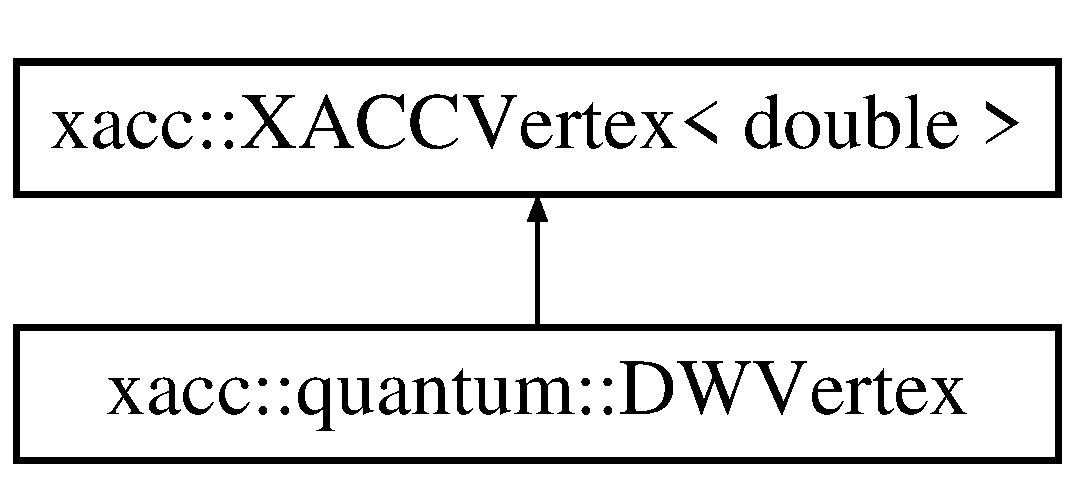
\includegraphics[height=2.000000cm]{a00049}
\end{center}
\end{figure}
\subsection*{Public Member Functions}
\begin{DoxyCompactItemize}
\item 
virtual std\+::shared\+\_\+ptr$<$ \hyperlink{a00038}{Function} $>$ \hyperlink{a00049_af42e466bf02dbd60670d20aa55cfb08d}{generate\+Algorithm} (std\+::vector$<$ int $>$ qubits)
\item 
virtual \hyperlink{a00049_a731c10d28046424be74e4c0daa31d016}{$\sim$\+Inverse\+Q\+FT} ()
\end{DoxyCompactItemize}


\subsection{Detailed Description}
\hyperlink{a00049}{Inverse\+Q\+FT} is a realization of the \hyperlink{a00014}{Algorithm\+Generator} interface that produces an X\+A\+CC \hyperlink{a00050}{IR} representation of the Inverse Quantum Fourier Transform. 

\subsection{Constructor \& Destructor Documentation}
\index{xacc\+::quantum\+::\+Inverse\+Q\+FT@{xacc\+::quantum\+::\+Inverse\+Q\+FT}!````~Inverse\+Q\+FT@{$\sim$\+Inverse\+Q\+FT}}
\index{````~Inverse\+Q\+FT@{$\sim$\+Inverse\+Q\+FT}!xacc\+::quantum\+::\+Inverse\+Q\+FT@{xacc\+::quantum\+::\+Inverse\+Q\+FT}}
\subsubsection[{\texorpdfstring{$\sim$\+Inverse\+Q\+F\+T()}{~InverseQFT()}}]{\setlength{\rightskip}{0pt plus 5cm}virtual xacc\+::quantum\+::\+Inverse\+Q\+F\+T\+::$\sim$\+Inverse\+Q\+FT (
\begin{DoxyParamCaption}
{}
\end{DoxyParamCaption}
)\hspace{0.3cm}{\ttfamily [inline]}, {\ttfamily [virtual]}}\hypertarget{a00049_a731c10d28046424be74e4c0daa31d016}{}\label{a00049_a731c10d28046424be74e4c0daa31d016}
The destructor 

\subsection{Member Function Documentation}
\index{xacc\+::quantum\+::\+Inverse\+Q\+FT@{xacc\+::quantum\+::\+Inverse\+Q\+FT}!generate\+Algorithm@{generate\+Algorithm}}
\index{generate\+Algorithm@{generate\+Algorithm}!xacc\+::quantum\+::\+Inverse\+Q\+FT@{xacc\+::quantum\+::\+Inverse\+Q\+FT}}
\subsubsection[{\texorpdfstring{generate\+Algorithm(std\+::vector$<$ int $>$ qubits)}{generateAlgorithm(std::vector< int > qubits)}}]{\setlength{\rightskip}{0pt plus 5cm}std\+::shared\+\_\+ptr$<$ {\bf Function} $>$ xacc\+::quantum\+::\+Inverse\+Q\+F\+T\+::generate\+Algorithm (
\begin{DoxyParamCaption}
\item[{std\+::vector$<$ int $>$}]{qubits}
\end{DoxyParamCaption}
)\hspace{0.3cm}{\ttfamily [virtual]}}\hypertarget{a00049_af42e466bf02dbd60670d20aa55cfb08d}{}\label{a00049_af42e466bf02dbd60670d20aa55cfb08d}
This implementation returns a \hyperlink{a00038}{Function} \hyperlink{a00050}{IR} representation of the inverse quantum fourier transform.


\begin{DoxyParams}{Parameters}
{\em bits} & The bits this algorithm operates on \\
\hline
\end{DoxyParams}
\begin{DoxyReturn}{Returns}
function The algorithm represented as an \hyperlink{a00050}{IR} \hyperlink{a00038}{Function} 
\end{DoxyReturn}


Implements \hyperlink{a00014_a73023c06f0f0c62ad56ab4187b18b096}{xacc\+::\+Algorithm\+Generator}.



The documentation for this class was generated from the following files\+:\begin{DoxyCompactItemize}
\item 
Inverse\+Q\+F\+T.\+hpp\item 
Inverse\+Q\+F\+T.\+cpp\end{DoxyCompactItemize}

\hypertarget{a00050}{}\section{case\+\_\+insensitive\+\_\+equals Class Reference}
\label{a00050}\index{case\+\_\+insensitive\+\_\+equals@{case\+\_\+insensitive\+\_\+equals}}
\subsection*{Public Member Functions}
\begin{DoxyCompactItemize}
\item 
bool {\bfseries operator()} (const std\+::string \&key1, const std\+::string \&key2) const \hypertarget{a00050_a4110d72a3ecfd3bd8ab698dd13c877d3}{}\label{a00050_a4110d72a3ecfd3bd8ab698dd13c877d3}

\item 
bool {\bfseries operator()} (const std\+::string \&key1, const std\+::string \&key2) const \hypertarget{a00050_a4110d72a3ecfd3bd8ab698dd13c877d3}{}\label{a00050_a4110d72a3ecfd3bd8ab698dd13c877d3}

\end{DoxyCompactItemize}


The documentation for this class was generated from the following files\+:\begin{DoxyCompactItemize}
\item 
client\+\_\+http.\+hpp\item 
server\+\_\+http.\+hpp\end{DoxyCompactItemize}

\hypertarget{a00051}{}\section{case\+\_\+insensitive\+\_\+hash Class Reference}
\label{a00051}\index{case\+\_\+insensitive\+\_\+hash@{case\+\_\+insensitive\+\_\+hash}}
\subsection*{Public Member Functions}
\begin{DoxyCompactItemize}
\item 
std\+::size\+\_\+t {\bfseries operator()} (const std\+::string \&key) const \hypertarget{a00051_a9969b2f956909125d5a83864a15736f4}{}\label{a00051_a9969b2f956909125d5a83864a15736f4}

\item 
size\+\_\+t {\bfseries operator()} (const std\+::string \&key) const \hypertarget{a00051_a1c9bbdf416c7580c3f9716abf5269746}{}\label{a00051_a1c9bbdf416c7580c3f9716abf5269746}

\end{DoxyCompactItemize}


The documentation for this class was generated from the following files\+:\begin{DoxyCompactItemize}
\item 
client\+\_\+http.\+hpp\item 
server\+\_\+http.\+hpp\end{DoxyCompactItemize}

\hypertarget{a00052}{}\section{xacc\+:\+:quantum\+:\+:Embedding\+Algorithm Class Reference}
\label{a00052}\index{xacc\+::quantum\+::\+Embedding\+Algorithm@{xacc\+::quantum\+::\+Embedding\+Algorithm}}


{\ttfamily \#include $<$Embedding\+Algorithm.\+hpp$>$}

Inheritance diagram for xacc\+:\+:quantum\+:\+:Embedding\+Algorithm\+:\begin{figure}[H]
\begin{center}
\leavevmode
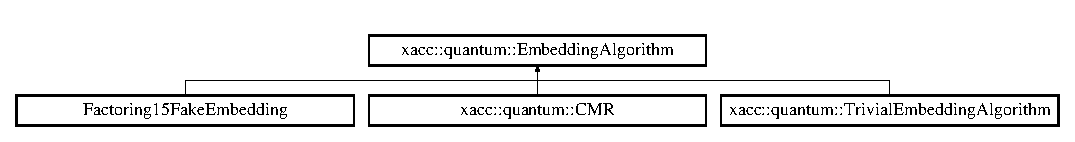
\includegraphics[height=1.464052cm]{a00052}
\end{center}
\end{figure}
\subsection*{Public Member Functions}
\begin{DoxyCompactItemize}
\item 
\hyperlink{a00052_abad06507eef6b63af0884e3a96145c69}{Embedding\+Algorithm} ()
\item 
virtual \hyperlink{a00052_aa43660ad5d4c4b3ac67863892c33dc51}{$\sim$\+Embedding\+Algorithm} ()
\item 
virtual std\+::map$<$ int, std\+::list$<$ int $>$ $>$ \hyperlink{a00052_a6fca277e217884ff79802770189276fe}{embed} (std\+::shared\+\_\+ptr$<$ \hyperlink{a00043}{D\+W\+Graph} $>$ problem, std\+::shared\+\_\+ptr$<$ \hyperlink{a00064}{Accelerator\+Graph} $>$ hardware, std\+::map$<$ std\+::string, std\+::string $>$ params=std\+::map$<$ std\+::string, std\+::string $>$())=0
\item 
virtual std\+::string \hyperlink{a00052_a21079dc8ee37792977f5fd209e3f3b19}{name} ()=0
\end{DoxyCompactItemize}


\subsection{Detailed Description}
The \hyperlink{a00052}{Embedding\+Algorithm} class provides an interface for minor graph embedding algorithms. 

\subsection{Constructor \& Destructor Documentation}
\index{xacc\+::quantum\+::\+Embedding\+Algorithm@{xacc\+::quantum\+::\+Embedding\+Algorithm}!Embedding\+Algorithm@{Embedding\+Algorithm}}
\index{Embedding\+Algorithm@{Embedding\+Algorithm}!xacc\+::quantum\+::\+Embedding\+Algorithm@{xacc\+::quantum\+::\+Embedding\+Algorithm}}
\subsubsection[{\texorpdfstring{Embedding\+Algorithm()}{EmbeddingAlgorithm()}}]{\setlength{\rightskip}{0pt plus 5cm}xacc\+::quantum\+::\+Embedding\+Algorithm\+::\+Embedding\+Algorithm (
\begin{DoxyParamCaption}
{}
\end{DoxyParamCaption}
)\hspace{0.3cm}{\ttfamily [inline]}}\hypertarget{a00052_abad06507eef6b63af0884e3a96145c69}{}\label{a00052_abad06507eef6b63af0884e3a96145c69}
The Constructor \index{xacc\+::quantum\+::\+Embedding\+Algorithm@{xacc\+::quantum\+::\+Embedding\+Algorithm}!````~Embedding\+Algorithm@{$\sim$\+Embedding\+Algorithm}}
\index{````~Embedding\+Algorithm@{$\sim$\+Embedding\+Algorithm}!xacc\+::quantum\+::\+Embedding\+Algorithm@{xacc\+::quantum\+::\+Embedding\+Algorithm}}
\subsubsection[{\texorpdfstring{$\sim$\+Embedding\+Algorithm()}{~EmbeddingAlgorithm()}}]{\setlength{\rightskip}{0pt plus 5cm}virtual xacc\+::quantum\+::\+Embedding\+Algorithm\+::$\sim$\+Embedding\+Algorithm (
\begin{DoxyParamCaption}
{}
\end{DoxyParamCaption}
)\hspace{0.3cm}{\ttfamily [inline]}, {\ttfamily [virtual]}}\hypertarget{a00052_aa43660ad5d4c4b3ac67863892c33dc51}{}\label{a00052_aa43660ad5d4c4b3ac67863892c33dc51}
The Destructor 

\subsection{Member Function Documentation}
\index{xacc\+::quantum\+::\+Embedding\+Algorithm@{xacc\+::quantum\+::\+Embedding\+Algorithm}!embed@{embed}}
\index{embed@{embed}!xacc\+::quantum\+::\+Embedding\+Algorithm@{xacc\+::quantum\+::\+Embedding\+Algorithm}}
\subsubsection[{\texorpdfstring{embed(std\+::shared\+\_\+ptr$<$ D\+W\+Graph $>$ problem, std\+::shared\+\_\+ptr$<$ Accelerator\+Graph $>$ hardware, std\+::map$<$ std\+::string, std\+::string $>$ params=std\+::map$<$ std\+::string, std\+::string $>$())=0}{embed(std::shared\_ptr< DWGraph > problem, std::shared\_ptr< AcceleratorGraph > hardware, std::map< std::string, std::string > params=std::map< std::string, std::string >())=0}}]{\setlength{\rightskip}{0pt plus 5cm}virtual std\+::map$<$int, std\+::list$<$int$>$ $>$ xacc\+::quantum\+::\+Embedding\+Algorithm\+::embed (
\begin{DoxyParamCaption}
\item[{std\+::shared\+\_\+ptr$<$ {\bf D\+W\+Graph} $>$}]{problem, }
\item[{std\+::shared\+\_\+ptr$<$ {\bf Accelerator\+Graph} $>$}]{hardware, }
\item[{std\+::map$<$ std\+::string, std\+::string $>$}]{params = {\ttfamily std\+:\+:map$<$~std\+:\+:string,~std\+:\+:string~$>$()}}
\end{DoxyParamCaption}
)\hspace{0.3cm}{\ttfamily [pure virtual]}}\hypertarget{a00052_a6fca277e217884ff79802770189276fe}{}\label{a00052_a6fca277e217884ff79802770189276fe}
Implementations of \hyperlink{a00052}{Embedding\+Algorithm} implement this method to provide a valid minor graph embedding of the given problem graph into the given hardware graph.


\begin{DoxyParams}{Parameters}
{\em problem} & The problem graph to be embedded into the hardware graph \\
\hline
{\em hardware} & The hardware graph. \\
\hline
{\em params} & Any key-\/value string parameters to influence the algorithm. \\
\hline
\end{DoxyParams}
\begin{DoxyReturn}{Returns}
embedding A mapping of problem vertex indices to the list of hardware vertices they map to 
\end{DoxyReturn}


Implemented in \hyperlink{a00127_a09e162a745528ffa3ea847dd5afee45b}{xacc\+::quantum\+::\+Trivial\+Embedding\+Algorithm}, and \hyperlink{a00032_a3408b5b72c426b4733ea4b0a19feb2f4}{xacc\+::quantum\+::\+C\+MR}.

\index{xacc\+::quantum\+::\+Embedding\+Algorithm@{xacc\+::quantum\+::\+Embedding\+Algorithm}!name@{name}}
\index{name@{name}!xacc\+::quantum\+::\+Embedding\+Algorithm@{xacc\+::quantum\+::\+Embedding\+Algorithm}}
\subsubsection[{\texorpdfstring{name()=0}{name()=0}}]{\setlength{\rightskip}{0pt plus 5cm}virtual std\+::string xacc\+::quantum\+::\+Embedding\+Algorithm\+::name (
\begin{DoxyParamCaption}
{}
\end{DoxyParamCaption}
)\hspace{0.3cm}{\ttfamily [pure virtual]}}\hypertarget{a00052_a21079dc8ee37792977f5fd209e3f3b19}{}\label{a00052_a21079dc8ee37792977f5fd209e3f3b19}
Return the name of this \hyperlink{a00051}{Embedding} Algorithm \begin{DoxyReturn}{Returns}

\end{DoxyReturn}


Implemented in \hyperlink{a00058_a2fc78d2c2960cb0900b9224c8a2baf61}{Factoring15\+Fake\+Embedding}, \hyperlink{a00127_a5d3e8c56b53cda9c682dedc534bf38fb}{xacc\+::quantum\+::\+Trivial\+Embedding\+Algorithm}, and \hyperlink{a00032_a06abf96899ccbfb4e2e0b2c72f978854}{xacc\+::quantum\+::\+C\+MR}.



The documentation for this class was generated from the following file\+:\begin{DoxyCompactItemize}
\item 
Embedding\+Algorithm.\+hpp\end{DoxyCompactItemize}

\hypertarget{a00053}{}\section{Embedding\+Algorithm\+Factory Class Reference}
\label{a00053}\index{Embedding\+Algorithm\+Factory@{Embedding\+Algorithm\+Factory}}


{\ttfamily \#include $<$Embedding\+Algorithm\+Factory.\+hpp$>$}

\subsection*{Public Member Functions}
\begin{DoxyCompactItemize}
\item 
std\+::shared\+\_\+ptr$<$ \hyperlink{a00071}{I\+Embedding\+Algorithm} $>$ \hyperlink{a00053_a19e9ec2636073705e65c1039c8879be7}{create\+Embedding\+Algorithm} (std\+::string type, \hyperlink{a00076}{I\+Quell\+E\+Graph} \&prob, \hyperlink{a00076}{I\+Quell\+E\+Graph} \&hardware)
\item 
{\footnotesize template$<$typename T $>$ }\\void \hyperlink{a00053_aec39e8d4edc3715f3980db5d13252f3b}{reg} (const std\+::string \&name)
\item 
std\+::vector$<$ std\+::string $>$ {\bfseries list\+Embedding\+Algorithms} ()\hypertarget{a00053_ab19e4f507f0ac05a0b37ae75c68b6df4}{}\label{a00053_ab19e4f507f0ac05a0b37ae75c68b6df4}

\end{DoxyCompactItemize}
\subsection*{Static Public Member Functions}
\begin{DoxyCompactItemize}
\item 
static std\+::shared\+\_\+ptr$<$ \hyperlink{a00053}{Embedding\+Algorithm\+Factory} $>$ \hyperlink{a00053_a1fccee9971df2df4870cd1333798b3da}{instance} ()
\end{DoxyCompactItemize}
\subsection*{Protected Member Functions}
\begin{DoxyCompactItemize}
\item 
\hyperlink{a00053_ac19af2c293caa47ea46a0122f3e81e28}{Embedding\+Algorithm\+Factory} ()
\end{DoxyCompactItemize}
\subsection*{Protected Attributes}
\begin{DoxyCompactItemize}
\item 
std\+::map$<$ std\+::string, build\+Ptr $>$ \hyperlink{a00053_aa3bbf5d1683ddd7194f981f0af67e95a}{registration\+Map}
\end{DoxyCompactItemize}
\subsection*{Static Protected Attributes}
\begin{DoxyCompactItemize}
\item 
static std\+::shared\+\_\+ptr$<$ \hyperlink{a00053}{Embedding\+Algorithm\+Factory} $>$ \hyperlink{a00053_ad675ae385b8ffb8fb4eafe0253967ed9}{factory\+Instance} = 0
\end{DoxyCompactItemize}


\subsection{Detailed Description}
The \hyperlink{a00053}{Embedding\+Algorithm\+Factory} is a singleton that dynamically registers I\+Embedding\+Algorithms and provides a mechanism for clients to create them by just knowing the string name of the class. 

\subsection{Constructor \& Destructor Documentation}
\index{Embedding\+Algorithm\+Factory@{Embedding\+Algorithm\+Factory}!Embedding\+Algorithm\+Factory@{Embedding\+Algorithm\+Factory}}
\index{Embedding\+Algorithm\+Factory@{Embedding\+Algorithm\+Factory}!Embedding\+Algorithm\+Factory@{Embedding\+Algorithm\+Factory}}
\subsubsection[{\texorpdfstring{Embedding\+Algorithm\+Factory()}{EmbeddingAlgorithmFactory()}}]{\setlength{\rightskip}{0pt plus 5cm}Embedding\+Algorithm\+Factory\+::\+Embedding\+Algorithm\+Factory (
\begin{DoxyParamCaption}
{}
\end{DoxyParamCaption}
)\hspace{0.3cm}{\ttfamily [inline]}, {\ttfamily [protected]}}\hypertarget{a00053_ac19af2c293caa47ea46a0122f3e81e28}{}\label{a00053_ac19af2c293caa47ea46a0122f3e81e28}
The Constructor 

\subsection{Member Function Documentation}
\index{Embedding\+Algorithm\+Factory@{Embedding\+Algorithm\+Factory}!create\+Embedding\+Algorithm@{create\+Embedding\+Algorithm}}
\index{create\+Embedding\+Algorithm@{create\+Embedding\+Algorithm}!Embedding\+Algorithm\+Factory@{Embedding\+Algorithm\+Factory}}
\subsubsection[{\texorpdfstring{create\+Embedding\+Algorithm(std\+::string type, I\+Quell\+E\+Graph \&prob, I\+Quell\+E\+Graph \&hardware)}{createEmbeddingAlgorithm(std::string type, IQuellEGraph \&prob, IQuellEGraph \&hardware)}}]{\setlength{\rightskip}{0pt plus 5cm}std\+::shared\+\_\+ptr$<${\bf I\+Embedding\+Algorithm}$>$ Embedding\+Algorithm\+Factory\+::create\+Embedding\+Algorithm (
\begin{DoxyParamCaption}
\item[{std\+::string}]{type, }
\item[{{\bf I\+Quell\+E\+Graph} \&}]{prob, }
\item[{{\bf I\+Quell\+E\+Graph} \&}]{hardware}
\end{DoxyParamCaption}
)\hspace{0.3cm}{\ttfamily [inline]}}\hypertarget{a00053_a19e9ec2636073705e65c1039c8879be7}{}\label{a00053_a19e9ec2636073705e65c1039c8879be7}
Create the \hyperlink{a00071}{I\+Embedding\+Algorithm} corresponding to the provided string type and problem/hardware graphs.


\begin{DoxyParams}{Parameters}
{\em type} & \\
\hline
{\em prob} & \\
\hline
{\em hardware} & \\
\hline
\end{DoxyParams}
\begin{DoxyReturn}{Returns}

\end{DoxyReturn}
\index{Embedding\+Algorithm\+Factory@{Embedding\+Algorithm\+Factory}!instance@{instance}}
\index{instance@{instance}!Embedding\+Algorithm\+Factory@{Embedding\+Algorithm\+Factory}}
\subsubsection[{\texorpdfstring{instance()}{instance()}}]{\setlength{\rightskip}{0pt plus 5cm}static std\+::shared\+\_\+ptr$<${\bf Embedding\+Algorithm\+Factory}$>$ Embedding\+Algorithm\+Factory\+::instance (
\begin{DoxyParamCaption}
{}
\end{DoxyParamCaption}
)\hspace{0.3cm}{\ttfamily [inline]}, {\ttfamily [static]}}\hypertarget{a00053_a1fccee9971df2df4870cd1333798b3da}{}\label{a00053_a1fccee9971df2df4870cd1333798b3da}
Return the singleton instance for this factory.

\begin{DoxyReturn}{Returns}

\end{DoxyReturn}
\index{Embedding\+Algorithm\+Factory@{Embedding\+Algorithm\+Factory}!reg@{reg}}
\index{reg@{reg}!Embedding\+Algorithm\+Factory@{Embedding\+Algorithm\+Factory}}
\subsubsection[{\texorpdfstring{reg(const std\+::string \&name)}{reg(const std::string \&name)}}]{\setlength{\rightskip}{0pt plus 5cm}template$<$typename T $>$ void Embedding\+Algorithm\+Factory\+::reg (
\begin{DoxyParamCaption}
\item[{const std\+::string \&}]{name}
\end{DoxyParamCaption}
)\hspace{0.3cm}{\ttfamily [inline]}}\hypertarget{a00053_aec39e8d4edc3715f3980db5d13252f3b}{}\label{a00053_aec39e8d4edc3715f3980db5d13252f3b}
Register a new \hyperlink{a00071}{I\+Embedding\+Algorithm} with the factory.


\begin{DoxyParams}{Parameters}
{\em name} & \\
\hline
\end{DoxyParams}


\subsection{Member Data Documentation}
\index{Embedding\+Algorithm\+Factory@{Embedding\+Algorithm\+Factory}!factory\+Instance@{factory\+Instance}}
\index{factory\+Instance@{factory\+Instance}!Embedding\+Algorithm\+Factory@{Embedding\+Algorithm\+Factory}}
\subsubsection[{\texorpdfstring{factory\+Instance}{factoryInstance}}]{\setlength{\rightskip}{0pt plus 5cm}std\+::shared\+\_\+ptr$<$ {\bf Embedding\+Algorithm\+Factory} $>$ Embedding\+Algorithm\+Factory\+::factory\+Instance = 0\hspace{0.3cm}{\ttfamily [static]}, {\ttfamily [protected]}}\hypertarget{a00053_ad675ae385b8ffb8fb4eafe0253967ed9}{}\label{a00053_ad675ae385b8ffb8fb4eafe0253967ed9}
Reference to the singleton instance \index{Embedding\+Algorithm\+Factory@{Embedding\+Algorithm\+Factory}!registration\+Map@{registration\+Map}}
\index{registration\+Map@{registration\+Map}!Embedding\+Algorithm\+Factory@{Embedding\+Algorithm\+Factory}}
\subsubsection[{\texorpdfstring{registration\+Map}{registrationMap}}]{\setlength{\rightskip}{0pt plus 5cm}std\+::map$<$std\+::string, build\+Ptr$>$ Embedding\+Algorithm\+Factory\+::registration\+Map\hspace{0.3cm}{\ttfamily [protected]}}\hypertarget{a00053_aa3bbf5d1683ddd7194f981f0af67e95a}{}\label{a00053_aa3bbf5d1683ddd7194f981f0af67e95a}
Reference to the registration map. 

The documentation for this class was generated from the following files\+:\begin{DoxyCompactItemize}
\item 
Embedding\+Algorithm\+Factory.\+hpp\item 
Embedding\+Algorithm\+Factory.\+cpp\end{DoxyCompactItemize}

\hypertarget{a00054}{}\section{xacc\+:\+:quantum\+:\+:K44\+Bipartite Class Reference}
\label{a00054}\index{xacc\+::quantum\+::\+K44\+Bipartite@{xacc\+::quantum\+::\+K44\+Bipartite}}
Inheritance diagram for xacc\+:\+:quantum\+:\+:K44\+Bipartite\+:\begin{figure}[H]
\begin{center}
\leavevmode
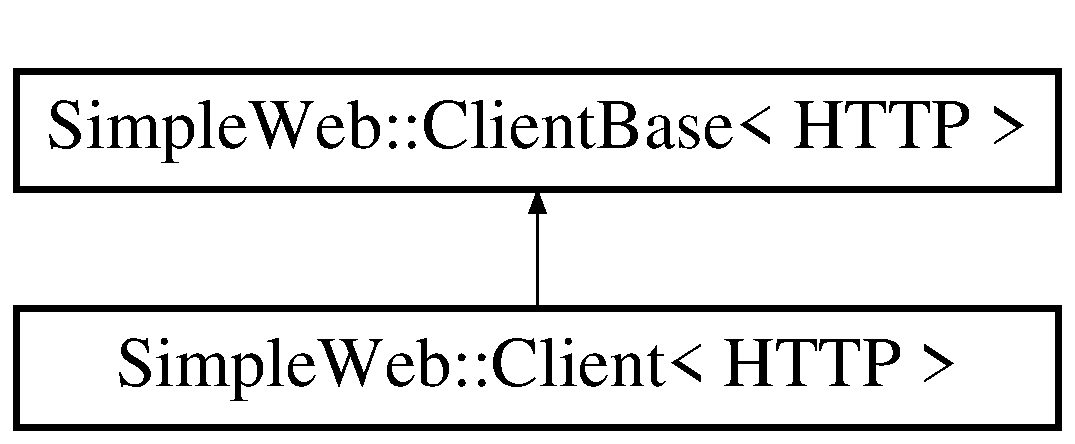
\includegraphics[height=3.000000cm]{a00054}
\end{center}
\end{figure}
\subsection*{Additional Inherited Members}


The documentation for this class was generated from the following file\+:\begin{DoxyCompactItemize}
\item 
D\+W\+Graph.\+hpp\end{DoxyCompactItemize}

\hypertarget{a00055}{}\section{xacc\+:\+:quantum\+:\+:Register\+Gate\+Instruction$<$ T $>$ Class Template Reference}
\label{a00055}\index{xacc\+::quantum\+::\+Register\+Gate\+Instruction$<$ T $>$@{xacc\+::quantum\+::\+Register\+Gate\+Instruction$<$ T $>$}}
\subsection*{Public Member Functions}
\begin{DoxyCompactItemize}
\item 
{\bfseries Register\+Gate\+Instruction} (const std\+::string \&name)\hypertarget{a00055_aad394924e098f0cc8da5cc7f211acd7a}{}\label{a00055_aad394924e098f0cc8da5cc7f211acd7a}

\end{DoxyCompactItemize}


The documentation for this class was generated from the following file\+:\begin{DoxyCompactItemize}
\item 
Gate\+Instruction.\+hpp\end{DoxyCompactItemize}

\hypertarget{a00056}{}\section{xacc\+:\+:Registry$<$ T, T\+Args $>$ Class Template Reference}
\label{a00056}\index{xacc\+::\+Registry$<$ T, T\+Args $>$@{xacc\+::\+Registry$<$ T, T\+Args $>$}}


{\ttfamily \#include $<$Registry.\+hpp$>$}

Inheritance diagram for xacc\+:\+:Registry$<$ T, T\+Args $>$\+:\begin{figure}[H]
\begin{center}
\leavevmode
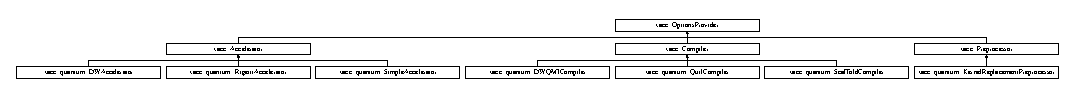
\includegraphics[height=2.000000cm]{a00056}
\end{center}
\end{figure}
\subsection*{Public Member Functions}
\begin{DoxyCompactItemize}
\item 
bool \hyperlink{a00056_a9aa172c2603171db067b40bd62ba53c6}{add} (const std\+::string \&id, std\+::function$<$ std\+::shared\+\_\+ptr$<$ T $>$(T\+Args...)$>$ f)
\item 
std\+::shared\+\_\+ptr$<$ T $>$ \hyperlink{a00056_aecccbd5534276cbdd1553e43c942219b}{create} (const std\+::string \&id, T\+Args...\+args)
\item 
std\+::vector$<$ std\+::string $>$ \hyperlink{a00056_a8bff6f5c50534375abc4026662d69d2e}{get\+Registered\+Ids} ()
\item 
std\+::size\+\_\+t \hyperlink{a00056_a2352dd7c6c85ae5c5e232b577dfa2544}{size} ()
\end{DoxyCompactItemize}
\subsection*{Protected Attributes}
\begin{DoxyCompactItemize}
\item 
std\+::map$<$ std\+::string, std\+::function$<$ std\+::shared\+\_\+ptr$<$ T $>$T\+Args...)$>$ $>$ \hyperlink{a00056_a46460ecacc7facb6936b3c1ec6d618d7}{registry}
\end{DoxyCompactItemize}
\subsection*{Additional Inherited Members}


\subsection{Detailed Description}
\subsubsection*{template$<$typename T, typename... T\+Args$>$\\*
class xacc\+::\+Registry$<$ T, T\+Args $>$}

\hyperlink{a00056}{Registry} is a \hyperlink{a00068}{Singleton} that provides a mapping of string ids to creation functions that create and return the provided \hyperlink{a00056}{Registry} template parameter T.

Clients can add new creation functions to be placed in the map with a unique name key, and can request that the \hyperlink{a00056}{Registry} return a new created instance of the template parameter T. 

\subsection{Member Function Documentation}
\index{xacc\+::\+Registry@{xacc\+::\+Registry}!add@{add}}
\index{add@{add}!xacc\+::\+Registry@{xacc\+::\+Registry}}
\subsubsection[{\texorpdfstring{add(const std\+::string \&id, std\+::function$<$ std\+::shared\+\_\+ptr$<$ T $>$(\+T\+Args...)$>$ f)}{add(const std::string \&id, std::function< std::shared\_ptr< T >(TArgs...)> f)}}]{\setlength{\rightskip}{0pt plus 5cm}template$<$typename T, typename... T\+Args$>$ bool {\bf xacc\+::\+Registry}$<$ T, T\+Args $>$\+::add (
\begin{DoxyParamCaption}
\item[{const std\+::string \&}]{id, }
\item[{std\+::function$<$ std\+::shared\+\_\+ptr$<$ T $>$(T\+Args...)$>$}]{f}
\end{DoxyParamCaption}
)\hspace{0.3cm}{\ttfamily [inline]}}\hypertarget{a00056_a9aa172c2603171db067b40bd62ba53c6}{}\label{a00056_a9aa172c2603171db067b40bd62ba53c6}
Add a new creation function to the \hyperlink{a00056}{Registry}, keyed on the provided string id.


\begin{DoxyParams}{Parameters}
{\em id} & The Id of the creation function \\
\hline
{\em f} & The object\textquotesingle{}s creation function \\
\hline
\end{DoxyParams}
\begin{DoxyReturn}{Returns}
success Bool indicating if this creator was added successfully. 
\end{DoxyReturn}
\index{xacc\+::\+Registry@{xacc\+::\+Registry}!create@{create}}
\index{create@{create}!xacc\+::\+Registry@{xacc\+::\+Registry}}
\subsubsection[{\texorpdfstring{create(const std\+::string \&id, T\+Args...\+args)}{create(const std::string \&id, TArgs...args)}}]{\setlength{\rightskip}{0pt plus 5cm}template$<$typename T, typename... T\+Args$>$ std\+::shared\+\_\+ptr$<$T$>$ {\bf xacc\+::\+Registry}$<$ T, T\+Args $>$\+::create (
\begin{DoxyParamCaption}
\item[{const std\+::string \&}]{id, }
\item[{T\+Args...}]{args}
\end{DoxyParamCaption}
)\hspace{0.3cm}{\ttfamily [inline]}}\hypertarget{a00056_aecccbd5534276cbdd1553e43c942219b}{}\label{a00056_aecccbd5534276cbdd1553e43c942219b}
Create an instance of T by using the creation function found at the given key string id.


\begin{DoxyParams}{Parameters}
{\em id} & The Id of the creation function \\
\hline
\end{DoxyParams}
\begin{DoxyReturn}{Returns}
object Shared Pointer for the created object. 
\end{DoxyReturn}
\index{xacc\+::\+Registry@{xacc\+::\+Registry}!get\+Registered\+Ids@{get\+Registered\+Ids}}
\index{get\+Registered\+Ids@{get\+Registered\+Ids}!xacc\+::\+Registry@{xacc\+::\+Registry}}
\subsubsection[{\texorpdfstring{get\+Registered\+Ids()}{getRegisteredIds()}}]{\setlength{\rightskip}{0pt plus 5cm}template$<$typename T, typename... T\+Args$>$ std\+::vector$<$std\+::string$>$ {\bf xacc\+::\+Registry}$<$ T, T\+Args $>$\+::get\+Registered\+Ids (
\begin{DoxyParamCaption}
{}
\end{DoxyParamCaption}
)\hspace{0.3cm}{\ttfamily [inline]}}\hypertarget{a00056_a8bff6f5c50534375abc4026662d69d2e}{}\label{a00056_a8bff6f5c50534375abc4026662d69d2e}
Return the keys from the registry map.

\begin{DoxyReturn}{Returns}
ids The registered creator Ids 
\end{DoxyReturn}
\index{xacc\+::\+Registry@{xacc\+::\+Registry}!size@{size}}
\index{size@{size}!xacc\+::\+Registry@{xacc\+::\+Registry}}
\subsubsection[{\texorpdfstring{size()}{size()}}]{\setlength{\rightskip}{0pt plus 5cm}template$<$typename T, typename... T\+Args$>$ std\+::size\+\_\+t {\bf xacc\+::\+Registry}$<$ T, T\+Args $>$\+::size (
\begin{DoxyParamCaption}
{}
\end{DoxyParamCaption}
)\hspace{0.3cm}{\ttfamily [inline]}}\hypertarget{a00056_a2352dd7c6c85ae5c5e232b577dfa2544}{}\label{a00056_a2352dd7c6c85ae5c5e232b577dfa2544}
Return the number of creation functions this registry contains.

\begin{DoxyReturn}{Returns}
size The number of creators in this \hyperlink{a00056}{Registry} 
\end{DoxyReturn}


\subsection{Member Data Documentation}
\index{xacc\+::\+Registry@{xacc\+::\+Registry}!registry@{registry}}
\index{registry@{registry}!xacc\+::\+Registry@{xacc\+::\+Registry}}
\subsubsection[{\texorpdfstring{registry}{registry}}]{\setlength{\rightskip}{0pt plus 5cm}template$<$typename T, typename... T\+Args$>$ std\+::map$<$std\+::string, std\+::function$<$std\+::shared\+\_\+ptr$<$T$>$T\+Args...)$>$ $>$ {\bf xacc\+::\+Registry}$<$ T, T\+Args $>$\+::registry\hspace{0.3cm}{\ttfamily [protected]}}\hypertarget{a00056_a46460ecacc7facb6936b3c1ec6d618d7}{}\label{a00056_a46460ecacc7facb6936b3c1ec6d618d7}
Reference to the database of creation functions for classes of superclass type T. 

The documentation for this class was generated from the following file\+:\begin{DoxyCompactItemize}
\item 
Registry.\+hpp\end{DoxyCompactItemize}

\hypertarget{a00057}{}\section{xacc\+:\+:Options\+Provider Class Reference}
\label{a00057}\index{xacc\+::\+Options\+Provider@{xacc\+::\+Options\+Provider}}


{\ttfamily \#include $<$Options\+Provider.\+hpp$>$}

Inheritance diagram for xacc\+:\+:Options\+Provider\+:\begin{figure}[H]
\begin{center}
\leavevmode
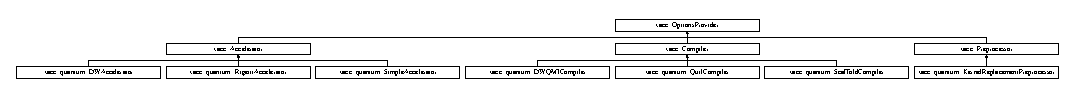
\includegraphics[height=0.824742cm]{a00057}
\end{center}
\end{figure}
\subsection*{Public Member Functions}
\begin{DoxyCompactItemize}
\item 
virtual std\+::shared\+\_\+ptr$<$ options\+\_\+description $>$ \hyperlink{a00057_a6d150954f852109bfe2c1ae90222926f}{get\+Options} ()=0
\item 
virtual \hyperlink{a00057_a7782757b419792ff346f563517eed8b8}{$\sim$\+Options\+Provider} ()
\end{DoxyCompactItemize}


\subsection{Detailed Description}
The \hyperlink{a00057}{Options\+Provider} interface enables derived subclasses to provide a description of any and all command line options that they can take to drive and control their execution and behavior. 

\subsection{Constructor \& Destructor Documentation}
\index{xacc\+::\+Options\+Provider@{xacc\+::\+Options\+Provider}!````~Options\+Provider@{$\sim$\+Options\+Provider}}
\index{````~Options\+Provider@{$\sim$\+Options\+Provider}!xacc\+::\+Options\+Provider@{xacc\+::\+Options\+Provider}}
\subsubsection[{\texorpdfstring{$\sim$\+Options\+Provider()}{~OptionsProvider()}}]{\setlength{\rightskip}{0pt plus 5cm}virtual xacc\+::\+Options\+Provider\+::$\sim$\+Options\+Provider (
\begin{DoxyParamCaption}
{}
\end{DoxyParamCaption}
)\hspace{0.3cm}{\ttfamily [inline]}, {\ttfamily [virtual]}}\hypertarget{a00057_a7782757b419792ff346f563517eed8b8}{}\label{a00057_a7782757b419792ff346f563517eed8b8}
The destructor 

\subsection{Member Function Documentation}
\index{xacc\+::\+Options\+Provider@{xacc\+::\+Options\+Provider}!get\+Options@{get\+Options}}
\index{get\+Options@{get\+Options}!xacc\+::\+Options\+Provider@{xacc\+::\+Options\+Provider}}
\subsubsection[{\texorpdfstring{get\+Options()=0}{getOptions()=0}}]{\setlength{\rightskip}{0pt plus 5cm}virtual std\+::shared\+\_\+ptr$<$options\+\_\+description$>$ xacc\+::\+Options\+Provider\+::get\+Options (
\begin{DoxyParamCaption}
{}
\end{DoxyParamCaption}
)\hspace{0.3cm}{\ttfamily [pure virtual]}}\hypertarget{a00057_a6d150954f852109bfe2c1ae90222926f}{}\label{a00057_a6d150954f852109bfe2c1ae90222926f}
Return a Boost options\+\_\+description instance that describes the options available for this derived subclass. 

Implemented in \hyperlink{a00011_a98c9eda6b54367c75667ecfbbf167979}{xacc\+::\+Accelerator}, \hyperlink{a00029_a09926db9f99706307ae6ce5b56845bca}{xacc\+::quantum\+::\+D\+W\+Accelerator}, \hyperlink{a00072_a9ee9e62aecbccf193894ca3388676f9f}{xacc\+::quantum\+::\+Rigetti\+Accelerator}, \hyperlink{a00023_a9f5a8965c9c2dd895016d18264ebbe92}{xacc\+::\+Compiler}, \hyperlink{a00034_a0851334cc33b5b1da2694150a0a1a43c}{xacc\+::quantum\+::\+D\+W\+Q\+M\+I\+Compiler}, and \hyperlink{a00058_a96f5600ea47628b66917c7b90250e7f1}{xacc\+::\+Preprocessor}.



The documentation for this class was generated from the following file\+:\begin{DoxyCompactItemize}
\item 
Options\+Provider.\+hpp\end{DoxyCompactItemize}

\hypertarget{a00058}{}\section{xacc\+:\+:Program Class Reference}
\label{a00058}\index{xacc\+::\+Program@{xacc\+::\+Program}}


{\ttfamily \#include $<$Program.\+hpp$>$}

\subsection*{Public Member Functions}
\begin{DoxyCompactItemize}
\item 
\hyperlink{a00058_a6d20079fde67a3ef145315e762249115}{Program} (std\+::shared\+\_\+ptr$<$ \hyperlink{a00011}{Accelerator} $>$ acc, const std\+::string \&source\+File)
\item 
{\footnotesize template$<$typename... Runtime\+Args$>$ }\\std\+::function$<$ void(std\+::shared\+\_\+ptr$<$ \hyperlink{a00013}{Accelerator\+Buffer} $>$, Runtime\+Args...)$>$ \hyperlink{a00058_abf5023c9f01cac8a506bdef86760e8f1}{get\+Kernel} (const std\+::string \&kernel\+Name)
\end{DoxyCompactItemize}
\subsection*{Protected Member Functions}
\begin{DoxyCompactItemize}
\item 
void \hyperlink{a00058_a53079c7886c0be065968bcf6674d1516}{build} ()
\end{DoxyCompactItemize}
\subsection*{Protected Attributes}
\begin{DoxyCompactItemize}
\item 
std\+::string \hyperlink{a00058_aae78160f9f9e52a3e0c9b342996a7202}{src}
\item 
std\+::shared\+\_\+ptr$<$ \hyperlink{a00011}{Accelerator} $>$ \hyperlink{a00058_a10c948629c84f23dd426c04a9a518155}{accelerator}
\item 
std\+::shared\+\_\+ptr$<$ \hyperlink{a00050}{IR} $>$ \hyperlink{a00058_a5681f0989fc1c3fced8e30e815d6511c}{xacc\+IR}
\item 
std\+::shared\+\_\+ptr$<$ \hyperlink{a00023}{Compiler} $>$ \hyperlink{a00058_a0d2ae2522bb0daad0eea7871fc4e2061}{compiler}
\end{DoxyCompactItemize}


\subsection{Detailed Description}
The \hyperlink{a00058}{Program} is the main entrypoint for the X\+A\+CC A\+PI. Users with accelerator kernels must construct a valid \hyperlink{a00058}{Program} to be compiled and executed on the attached accelerator. Programs must be given the \hyperlink{a00011}{Accelerator} reference to be used and kernel source code at construction time. 

\subsection{Constructor \& Destructor Documentation}
\index{xacc\+::\+Program@{xacc\+::\+Program}!Program@{Program}}
\index{Program@{Program}!xacc\+::\+Program@{xacc\+::\+Program}}
\subsubsection[{\texorpdfstring{Program(std\+::shared\+\_\+ptr$<$ Accelerator $>$ acc, const std\+::string \&source\+File)}{Program(std::shared\_ptr< Accelerator > acc, const std::string \&sourceFile)}}]{\setlength{\rightskip}{0pt plus 5cm}xacc\+::\+Program\+::\+Program (
\begin{DoxyParamCaption}
\item[{std\+::shared\+\_\+ptr$<$ {\bf Accelerator} $>$}]{acc, }
\item[{const std\+::string \&}]{source\+File}
\end{DoxyParamCaption}
)\hspace{0.3cm}{\ttfamily [inline]}}\hypertarget{a00058_a6d20079fde67a3ef145315e762249115}{}\label{a00058_a6d20079fde67a3ef145315e762249115}
The Constructor, takes the \hyperlink{a00011}{Accelerator} to execute on, and the source to compile and execute


\begin{DoxyParams}{Parameters}
{\em acc} & Attached \hyperlink{a00011}{Accelerator} to execute \\
\hline
{\em source\+File} & The kernel source code \\
\hline
\end{DoxyParams}


\subsection{Member Function Documentation}
\index{xacc\+::\+Program@{xacc\+::\+Program}!build@{build}}
\index{build@{build}!xacc\+::\+Program@{xacc\+::\+Program}}
\subsubsection[{\texorpdfstring{build()}{build()}}]{\setlength{\rightskip}{0pt plus 5cm}void xacc\+::\+Program\+::build (
\begin{DoxyParamCaption}
{}
\end{DoxyParamCaption}
)\hspace{0.3cm}{\ttfamily [inline]}, {\ttfamily [protected]}}\hypertarget{a00058_a53079c7886c0be065968bcf6674d1516}{}\label{a00058_a53079c7886c0be065968bcf6674d1516}
Execute the compilation mechanism on the provided program source kernel code to produce X\+A\+CC \hyperlink{a00050}{IR} that can be executed on the attached \hyperlink{a00011}{Accelerator}. \index{xacc\+::\+Program@{xacc\+::\+Program}!get\+Kernel@{get\+Kernel}}
\index{get\+Kernel@{get\+Kernel}!xacc\+::\+Program@{xacc\+::\+Program}}
\subsubsection[{\texorpdfstring{get\+Kernel(const std\+::string \&kernel\+Name)}{getKernel(const std::string \&kernelName)}}]{\setlength{\rightskip}{0pt plus 5cm}template$<$typename... Runtime\+Args$>$ std\+::function$<$void(std\+::shared\+\_\+ptr$<${\bf Accelerator\+Buffer}$>$, Runtime\+Args...)$>$ xacc\+::\+Program\+::get\+Kernel (
\begin{DoxyParamCaption}
\item[{const std\+::string \&}]{kernel\+Name}
\end{DoxyParamCaption}
)\hspace{0.3cm}{\ttfamily [inline]}}\hypertarget{a00058_abf5023c9f01cac8a506bdef86760e8f1}{}\label{a00058_abf5023c9f01cac8a506bdef86760e8f1}
Return an executable version of the quantum kernel referenced by the kernel\+Name string.


\begin{DoxyParams}{Parameters}
{\em name} & \\
\hline
{\em args} & \\
\hline
\end{DoxyParams}
\begin{DoxyReturn}{Returns}

\end{DoxyReturn}


\subsection{Member Data Documentation}
\index{xacc\+::\+Program@{xacc\+::\+Program}!accelerator@{accelerator}}
\index{accelerator@{accelerator}!xacc\+::\+Program@{xacc\+::\+Program}}
\subsubsection[{\texorpdfstring{accelerator}{accelerator}}]{\setlength{\rightskip}{0pt plus 5cm}std\+::shared\+\_\+ptr$<${\bf Accelerator}$>$ xacc\+::\+Program\+::accelerator\hspace{0.3cm}{\ttfamily [protected]}}\hypertarget{a00058_a10c948629c84f23dd426c04a9a518155}{}\label{a00058_a10c948629c84f23dd426c04a9a518155}
Reference to the attached \hyperlink{a00011}{Accelerator} to use in this compilation and execution \index{xacc\+::\+Program@{xacc\+::\+Program}!compiler@{compiler}}
\index{compiler@{compiler}!xacc\+::\+Program@{xacc\+::\+Program}}
\subsubsection[{\texorpdfstring{compiler}{compiler}}]{\setlength{\rightskip}{0pt plus 5cm}std\+::shared\+\_\+ptr$<${\bf Compiler}$>$ xacc\+::\+Program\+::compiler\hspace{0.3cm}{\ttfamily [protected]}}\hypertarget{a00058_a0d2ae2522bb0daad0eea7871fc4e2061}{}\label{a00058_a0d2ae2522bb0daad0eea7871fc4e2061}
Reference to the compiler \index{xacc\+::\+Program@{xacc\+::\+Program}!src@{src}}
\index{src@{src}!xacc\+::\+Program@{xacc\+::\+Program}}
\subsubsection[{\texorpdfstring{src}{src}}]{\setlength{\rightskip}{0pt plus 5cm}std\+::string xacc\+::\+Program\+::src\hspace{0.3cm}{\ttfamily [protected]}}\hypertarget{a00058_aae78160f9f9e52a3e0c9b342996a7202}{}\label{a00058_aae78160f9f9e52a3e0c9b342996a7202}
Reference to the source accelerator kernel code to be compiled and executed \index{xacc\+::\+Program@{xacc\+::\+Program}!xacc\+IR@{xacc\+IR}}
\index{xacc\+IR@{xacc\+IR}!xacc\+::\+Program@{xacc\+::\+Program}}
\subsubsection[{\texorpdfstring{xacc\+IR}{xaccIR}}]{\setlength{\rightskip}{0pt plus 5cm}std\+::shared\+\_\+ptr$<${\bf IR}$>$ xacc\+::\+Program\+::xacc\+IR\hspace{0.3cm}{\ttfamily [protected]}}\hypertarget{a00058_a5681f0989fc1c3fced8e30e815d6511c}{}\label{a00058_a5681f0989fc1c3fced8e30e815d6511c}
Reference to the X\+A\+CC \hyperlink{a00050}{IR} instance that is created by the \hyperlink{a00023}{Compiler} 

The documentation for this class was generated from the following file\+:\begin{DoxyCompactItemize}
\item 
Program.\+hpp\end{DoxyCompactItemize}

\hypertarget{a00059}{}\section{xacc\+:\+:runtime\+\_\+get\+\_\+func\+\_\+table$<$ Tuple, std\+:\+:index\+\_\+sequence$<$ Indices... $>$ $>$ Struct Template Reference}
\label{a00059}\index{xacc\+::runtime\+\_\+get\+\_\+func\+\_\+table$<$ Tuple, std\+::index\+\_\+sequence$<$ Indices... $>$ $>$@{xacc\+::runtime\+\_\+get\+\_\+func\+\_\+table$<$ Tuple, std\+::index\+\_\+sequence$<$ Indices... $>$ $>$}}
\subsection*{Public Types}
\begin{DoxyCompactItemize}
\item 
using {\bfseries return\+\_\+type} = typename std\+::tuple\+\_\+element$<$ 0, Tuple $>$\+::type \&\hypertarget{a00059_a1d2e9cd7910527e3c4f0162500f067a7}{}\label{a00059_a1d2e9cd7910527e3c4f0162500f067a7}

\item 
using {\bfseries get\+\_\+func\+\_\+ptr} = return\+\_\+type($\ast$)(Tuple \&) noexcept\hypertarget{a00059_afba5cf89694dc07b12aaabf6388a4427}{}\label{a00059_afba5cf89694dc07b12aaabf6388a4427}

\end{DoxyCompactItemize}
\subsection*{Static Public Attributes}
\begin{DoxyCompactItemize}
\item 
static constexpr get\+\_\+func\+\_\+ptr {\bfseries table} \mbox{[}std\+::tuple\+\_\+size$<$ Tuple $>$\+::value\mbox{]}
\end{DoxyCompactItemize}


\subsection{Member Data Documentation}
\index{xacc\+::runtime\+\_\+get\+\_\+func\+\_\+table$<$ Tuple, std\+::index\+\_\+sequence$<$ Indices... $>$ $>$@{xacc\+::runtime\+\_\+get\+\_\+func\+\_\+table$<$ Tuple, std\+::index\+\_\+sequence$<$ Indices... $>$ $>$}!table@{table}}
\index{table@{table}!xacc\+::runtime\+\_\+get\+\_\+func\+\_\+table$<$ Tuple, std\+::index\+\_\+sequence$<$ Indices... $>$ $>$@{xacc\+::runtime\+\_\+get\+\_\+func\+\_\+table$<$ Tuple, std\+::index\+\_\+sequence$<$ Indices... $>$ $>$}}
\subsubsection[{\texorpdfstring{table}{table}}]{\setlength{\rightskip}{0pt plus 5cm}template$<$typename Tuple , size\+\_\+t... Indices$>$ constexpr {\bf runtime\+\_\+get\+\_\+func\+\_\+table}$<$ Tuple, std\+::index\+\_\+sequence$<$ Indices... $>$ $>$\+::get\+\_\+func\+\_\+ptr {\bf xacc\+::runtime\+\_\+get\+\_\+func\+\_\+table}$<$ Tuple, std\+::index\+\_\+sequence$<$ Indices... $>$ $>$\+::table\hspace{0.3cm}{\ttfamily [static]}}\hypertarget{a00059_a80921470cc04db92bab9127ae768d759}{}\label{a00059_a80921470cc04db92bab9127ae768d759}
{\bfseries Initial value\+:}
\begin{DoxyCode}
=\{
        &std::get<Indices>...
    \}
\end{DoxyCode}


The documentation for this struct was generated from the following file\+:\begin{DoxyCompactItemize}
\item 
Utils.\+hpp\end{DoxyCompactItemize}

\hypertarget{a00060}{}\section{xacc\+:\+:quantum\+:\+:Functional\+Gate\+Instruction\+Visitor Class Reference}
\label{a00060}\index{xacc\+::quantum\+::\+Functional\+Gate\+Instruction\+Visitor@{xacc\+::quantum\+::\+Functional\+Gate\+Instruction\+Visitor}}
Inheritance diagram for xacc\+:\+:quantum\+:\+:Functional\+Gate\+Instruction\+Visitor\+:\begin{figure}[H]
\begin{center}
\leavevmode
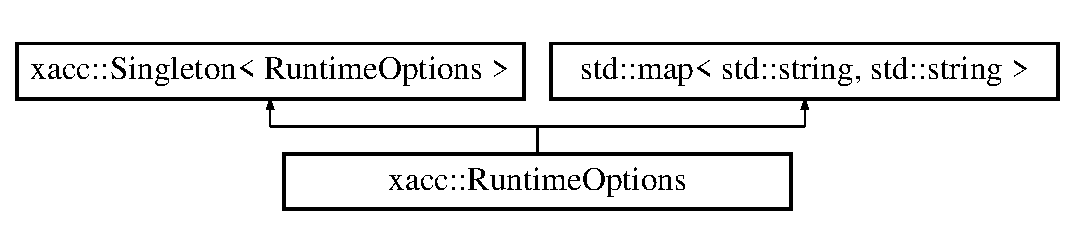
\includegraphics[height=12.000000cm]{a00060}
\end{center}
\end{figure}
\subsection*{Public Member Functions}
\begin{DoxyCompactItemize}
\item 
{\footnotesize template$<$typename HF , typename C\+NF , typename XF , typename YF , typename ZF , typename R\+XF , typename R\+YF , typename R\+ZF , typename MF , typename CF , typename C\+PF , typename S\+W\+A\+PF $>$ }\\{\bfseries Functional\+Gate\+Instruction\+Visitor} (HF h, C\+NF cn, XF x, YF y, ZF z, R\+XF rx, R\+YF ry, R\+ZF rz, MF m, CF c, C\+PF cp, S\+W\+A\+PF sw)\hypertarget{a00060_a4e3c27cd6b1acf063967b7b09a1eca09}{}\label{a00060_a4e3c27cd6b1acf063967b7b09a1eca09}

\item 
void {\bfseries visit} (\hyperlink{a00066}{Hadamard} \&h)\hypertarget{a00060_ac5245d34429dc112e7cd0e371108fcb5}{}\label{a00060_ac5245d34429dc112e7cd0e371108fcb5}

\item 
void {\bfseries visit} (\hyperlink{a00033}{C\+N\+OT} \&cn)\hypertarget{a00060_ad4eddafe8ca3906cd4aa5b98087a789a}{}\label{a00060_ad4eddafe8ca3906cd4aa5b98087a789a}

\item 
void {\bfseries visit} (\hyperlink{a00131}{X} \&x)\hypertarget{a00060_ac5d184daee7e755c9ede67b34bc2d091}{}\label{a00060_ac5d184daee7e755c9ede67b34bc2d091}

\item 
void {\bfseries visit} (\hyperlink{a00134}{Y} \&y)\hypertarget{a00060_a11dfa753a155346a45d7116a78c8f39f}{}\label{a00060_a11dfa753a155346a45d7116a78c8f39f}

\item 
void {\bfseries visit} (\hyperlink{a00135}{Z} \&z)\hypertarget{a00060_a4baf19da581fa9875739a227aba9cf60}{}\label{a00060_a4baf19da581fa9875739a227aba9cf60}

\item 
void {\bfseries visit} (\hyperlink{a00085}{Measure} \&m)\hypertarget{a00060_ad946faf8e2b6eff3e9e142907ec8e05a}{}\label{a00060_ad946faf8e2b6eff3e9e142907ec8e05a}

\item 
void {\bfseries visit} (\hyperlink{a00037}{Conditional\+Function} \&c)\hypertarget{a00060_a5cdb38902c241e7ae672a2631f1d61f3}{}\label{a00060_a5cdb38902c241e7ae672a2631f1d61f3}

\item 
void {\bfseries visit} (\hyperlink{a00114}{Rx} \&rx)\hypertarget{a00060_a6eb99e4b488773c750b7d9734ac1e885}{}\label{a00060_a6eb99e4b488773c750b7d9734ac1e885}

\item 
void {\bfseries visit} (\hyperlink{a00115}{Ry} \&ry)\hypertarget{a00060_aa22aad7b316386f5ef35672337c05ffc}{}\label{a00060_aa22aad7b316386f5ef35672337c05ffc}

\item 
void {\bfseries visit} (\hyperlink{a00040}{C\+Phase} \&cp)\hypertarget{a00060_a5475eece7afe380512a1a0215b92d302}{}\label{a00060_a5475eece7afe380512a1a0215b92d302}

\item 
void {\bfseries visit} (\hyperlink{a00116}{Rz} \&rz)\hypertarget{a00060_a8857ecf8f8f1b6143da8f31a722fe03e}{}\label{a00060_a8857ecf8f8f1b6143da8f31a722fe03e}

\item 
void {\bfseries visit} (\hyperlink{a00061}{Gate\+Function} \&f)\hypertarget{a00060_ad7d15225cf258fe59660ba828baff357}{}\label{a00060_ad7d15225cf258fe59660ba828baff357}

\item 
void {\bfseries visit} (\hyperlink{a00126}{Swap} \&s)\hypertarget{a00060_a30f46be43607813996c9cc090c1a5a16}{}\label{a00060_a30f46be43607813996c9cc090c1a5a16}

\end{DoxyCompactItemize}
\subsection*{Protected Attributes}
\begin{DoxyCompactItemize}
\item 
std\+::function$<$ void(\hyperlink{a00066}{Hadamard} \&)$>$ {\bfseries h\+Action}\hypertarget{a00060_a02f1401c9b0d1da801027f3bc0b5227e}{}\label{a00060_a02f1401c9b0d1da801027f3bc0b5227e}

\item 
std\+::function$<$ void(\hyperlink{a00033}{C\+N\+OT} \&)$>$ {\bfseries cnot\+Action}\hypertarget{a00060_a4d6bd8c2fd1af775ed08946942f60a0b}{}\label{a00060_a4d6bd8c2fd1af775ed08946942f60a0b}

\item 
std\+::function$<$ void(\hyperlink{a00131}{X} \&)$>$ {\bfseries x\+Action}\hypertarget{a00060_a9e0295434a2224b776609b057147a9af}{}\label{a00060_a9e0295434a2224b776609b057147a9af}

\item 
std\+::function$<$ void(\hyperlink{a00134}{Y} \&)$>$ {\bfseries y\+Action}\hypertarget{a00060_ae78f91a5cc9a7006f6bb1acee1c00501}{}\label{a00060_ae78f91a5cc9a7006f6bb1acee1c00501}

\item 
std\+::function$<$ void(\hyperlink{a00135}{Z} \&)$>$ {\bfseries z\+Action}\hypertarget{a00060_ae197f358e3d0777feb3656455e2ee672}{}\label{a00060_ae197f358e3d0777feb3656455e2ee672}

\item 
std\+::function$<$ void(\hyperlink{a00085}{Measure} \&)$>$ {\bfseries measure\+Action}\hypertarget{a00060_a239748abedd67c7b30cad12e545d1926}{}\label{a00060_a239748abedd67c7b30cad12e545d1926}

\item 
std\+::function$<$ void(\hyperlink{a00037}{Conditional\+Function} \&)$>$ {\bfseries cond\+Action}\hypertarget{a00060_a5c0595a70b1f7ae50f3e29a985e249e9}{}\label{a00060_a5c0595a70b1f7ae50f3e29a985e249e9}

\item 
std\+::function$<$ void(\hyperlink{a00114}{Rx} \&)$>$ {\bfseries rx\+Action}\hypertarget{a00060_ab79bb3eb3050d1c599061863bb2e219e}{}\label{a00060_ab79bb3eb3050d1c599061863bb2e219e}

\item 
std\+::function$<$ void(\hyperlink{a00115}{Ry} \&)$>$ {\bfseries ry\+Action}\hypertarget{a00060_a229b7d9aae52638c6eff04bd16bb9973}{}\label{a00060_a229b7d9aae52638c6eff04bd16bb9973}

\item 
std\+::function$<$ void(\hyperlink{a00116}{Rz} \&)$>$ {\bfseries rz\+Action}\hypertarget{a00060_a586ab5721150c67ad3ced46e2a236b44}{}\label{a00060_a586ab5721150c67ad3ced46e2a236b44}

\item 
std\+::function$<$ void(\hyperlink{a00040}{C\+Phase} \&)$>$ {\bfseries cp\+Action}\hypertarget{a00060_a5b88a0c9789e7b6d44527b2df6819ac5}{}\label{a00060_a5b88a0c9789e7b6d44527b2df6819ac5}

\item 
std\+::function$<$ void(\hyperlink{a00126}{Swap} \&)$>$ {\bfseries sw\+Action}\hypertarget{a00060_a5060cd4c2b1b259e32bda0e7ecc78e85}{}\label{a00060_a5060cd4c2b1b259e32bda0e7ecc78e85}

\end{DoxyCompactItemize}


The documentation for this class was generated from the following file\+:\begin{DoxyCompactItemize}
\item 
Functional\+Gate\+Instruction\+Visitor.\+hpp\end{DoxyCompactItemize}

\hypertarget{a00061}{}\section{xacc\+:\+:quantum\+:\+:Q\+FT Class Reference}
\label{a00061}\index{xacc\+::quantum\+::\+Q\+FT@{xacc\+::quantum\+::\+Q\+FT}}


{\ttfamily \#include $<$Q\+F\+T.\+hpp$>$}

Inheritance diagram for xacc\+:\+:quantum\+:\+:Q\+FT\+:\begin{figure}[H]
\begin{center}
\leavevmode
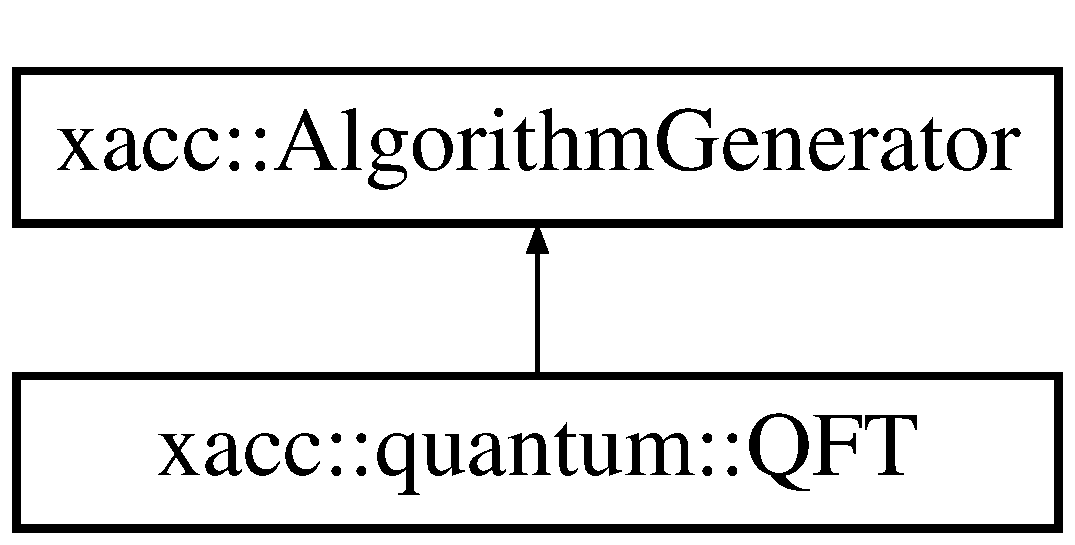
\includegraphics[height=2.000000cm]{a00061}
\end{center}
\end{figure}
\subsection*{Public Member Functions}
\begin{DoxyCompactItemize}
\item 
virtual std\+::shared\+\_\+ptr$<$ \hyperlink{a00039}{Function} $>$ \hyperlink{a00061_ac093c288bc9fc069464fc3fd2cc0ac21}{generate\+Algorithm} (std\+::vector$<$ int $>$ qubits)
\item 
virtual \hyperlink{a00061_a2f585738386f9a3744498983cd1f094e}{$\sim$\+Q\+FT} ()
\end{DoxyCompactItemize}


\subsection{Detailed Description}
\hyperlink{a00061}{Q\+FT} is a realization of the \hyperlink{a00014}{Algorithm\+Generator} interface that produces an X\+A\+CC \hyperlink{a00051}{IR} representation of the Quantum Fourier Transform.

\begin{DoxyAuthor}{Author}
Alex Mc\+Caskey 
\end{DoxyAuthor}


\subsection{Constructor \& Destructor Documentation}
\index{xacc\+::quantum\+::\+Q\+FT@{xacc\+::quantum\+::\+Q\+FT}!````~Q\+FT@{$\sim$\+Q\+FT}}
\index{````~Q\+FT@{$\sim$\+Q\+FT}!xacc\+::quantum\+::\+Q\+FT@{xacc\+::quantum\+::\+Q\+FT}}
\subsubsection[{\texorpdfstring{$\sim$\+Q\+F\+T()}{~QFT()}}]{\setlength{\rightskip}{0pt plus 5cm}virtual xacc\+::quantum\+::\+Q\+F\+T\+::$\sim$\+Q\+FT (
\begin{DoxyParamCaption}
{}
\end{DoxyParamCaption}
)\hspace{0.3cm}{\ttfamily [inline]}, {\ttfamily [virtual]}}\hypertarget{a00061_a2f585738386f9a3744498983cd1f094e}{}\label{a00061_a2f585738386f9a3744498983cd1f094e}
The destructor 

\subsection{Member Function Documentation}
\index{xacc\+::quantum\+::\+Q\+FT@{xacc\+::quantum\+::\+Q\+FT}!generate\+Algorithm@{generate\+Algorithm}}
\index{generate\+Algorithm@{generate\+Algorithm}!xacc\+::quantum\+::\+Q\+FT@{xacc\+::quantum\+::\+Q\+FT}}
\subsubsection[{\texorpdfstring{generate\+Algorithm(std\+::vector$<$ int $>$ qubits)}{generateAlgorithm(std::vector< int > qubits)}}]{\setlength{\rightskip}{0pt plus 5cm}std\+::shared\+\_\+ptr$<$ {\bf Function} $>$ xacc\+::quantum\+::\+Q\+F\+T\+::generate\+Algorithm (
\begin{DoxyParamCaption}
\item[{std\+::vector$<$ int $>$}]{qubits}
\end{DoxyParamCaption}
)\hspace{0.3cm}{\ttfamily [virtual]}}\hypertarget{a00061_ac093c288bc9fc069464fc3fd2cc0ac21}{}\label{a00061_ac093c288bc9fc069464fc3fd2cc0ac21}
This implementation returns a \hyperlink{a00039}{Function} \hyperlink{a00051}{IR} representation of the quantum fourier transform.


\begin{DoxyParams}{Parameters}
{\em bits} & The bits this algorithm operates on \\
\hline
\end{DoxyParams}
\begin{DoxyReturn}{Returns}
function The algorithm represented as an \hyperlink{a00051}{IR} \hyperlink{a00039}{Function} 
\end{DoxyReturn}


Implements \hyperlink{a00014_a73023c06f0f0c62ad56ab4187b18b096}{xacc\+::\+Algorithm\+Generator}.



The documentation for this class was generated from the following files\+:\begin{DoxyCompactItemize}
\item 
Q\+F\+T.\+hpp\item 
Q\+F\+T.\+cpp\end{DoxyCompactItemize}

\hypertarget{a00062}{}\section{xacc\+:\+:quantum\+:\+:Quantum\+Circuit Class Reference}
\label{a00062}\index{xacc\+::quantum\+::\+Quantum\+Circuit@{xacc\+::quantum\+::\+Quantum\+Circuit}}


{\ttfamily \#include $<$Quantum\+Circuit.\+hpp$>$}

Inheritance diagram for xacc\+:\+:quantum\+:\+:Quantum\+Circuit\+:\begin{figure}[H]
\begin{center}
\leavevmode
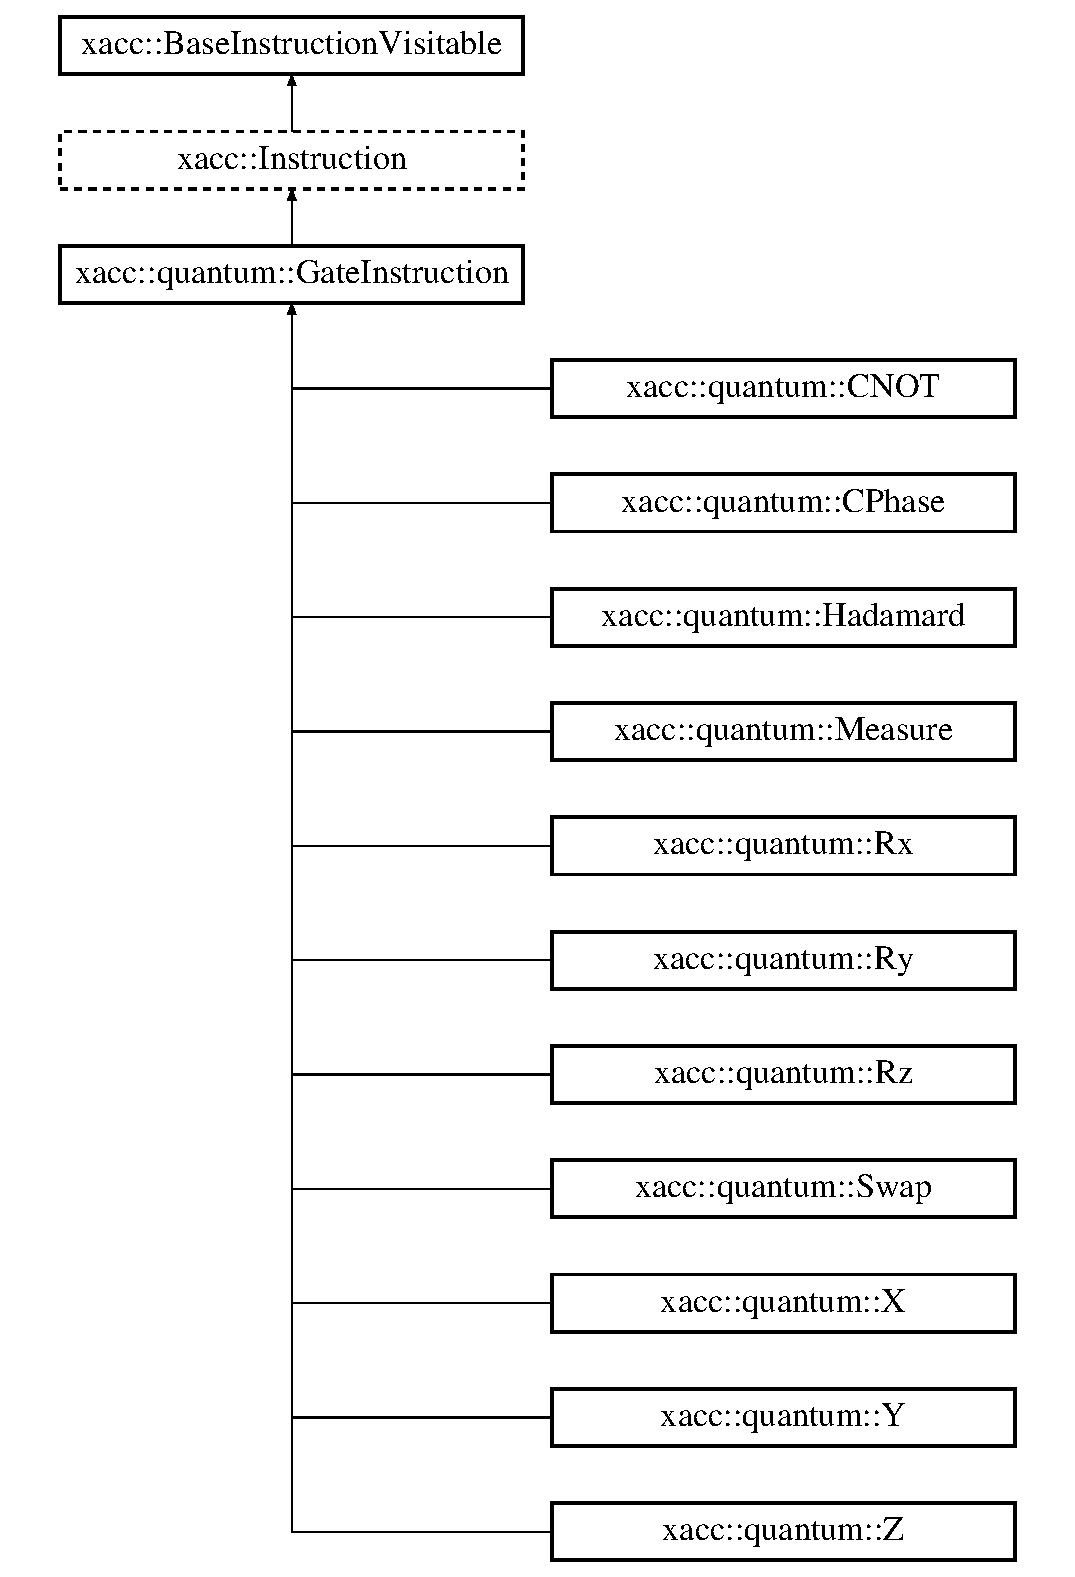
\includegraphics[height=2.000000cm]{a00062}
\end{center}
\end{figure}
\subsection*{Public Member Functions}
\begin{DoxyCompactItemize}
\item 
virtual void \hyperlink{a00062_af7a7f4a487d493fe8a4ed1f76cefd731}{read} (std\+::istream \&stream)
\end{DoxyCompactItemize}
\subsection*{Additional Inherited Members}


\subsection{Detailed Description}
The \hyperlink{a00062}{Quantum\+Circuit} is a subclass of \hyperlink{a00044}{Graph} that provides its Vertex template parameter as a \hyperlink{a00020}{Circuit\+Node}. It adds the ability to read Quantum\+Circuits from a graphviz dot file. 

\subsection{Member Function Documentation}
\index{xacc\+::quantum\+::\+Quantum\+Circuit@{xacc\+::quantum\+::\+Quantum\+Circuit}!read@{read}}
\index{read@{read}!xacc\+::quantum\+::\+Quantum\+Circuit@{xacc\+::quantum\+::\+Quantum\+Circuit}}
\subsubsection[{\texorpdfstring{read(std\+::istream \&stream)}{read(std::istream \&stream)}}]{\setlength{\rightskip}{0pt plus 5cm}virtual void xacc\+::quantum\+::\+Quantum\+Circuit\+::read (
\begin{DoxyParamCaption}
\item[{std\+::istream \&}]{stream}
\end{DoxyParamCaption}
)\hspace{0.3cm}{\ttfamily [inline]}, {\ttfamily [virtual]}}\hypertarget{a00062_af7a7f4a487d493fe8a4ed1f76cefd731}{}\label{a00062_af7a7f4a487d493fe8a4ed1f76cefd731}
Read in a graphviz dot graph from the given input stream. This is left for subclasses.


\begin{DoxyParams}{Parameters}
{\em stream} & \\
\hline
\end{DoxyParams}


Reimplemented from \hyperlink{a00044_abdd3e67dc08c223821d809bc8914164a}{xacc\+::\+Graph$<$ Circuit\+Node $>$}.



The documentation for this class was generated from the following file\+:\begin{DoxyCompactItemize}
\item 
Quantum\+Circuit.\+hpp\end{DoxyCompactItemize}

\hypertarget{a00063}{}\section{xacc\+:\+:quantum\+:\+:Quil\+Compiler Class Reference}
\label{a00063}\index{xacc\+::quantum\+::\+Quil\+Compiler@{xacc\+::quantum\+::\+Quil\+Compiler}}
Inheritance diagram for xacc\+:\+:quantum\+:\+:Quil\+Compiler\+:\begin{figure}[H]
\begin{center}
\leavevmode
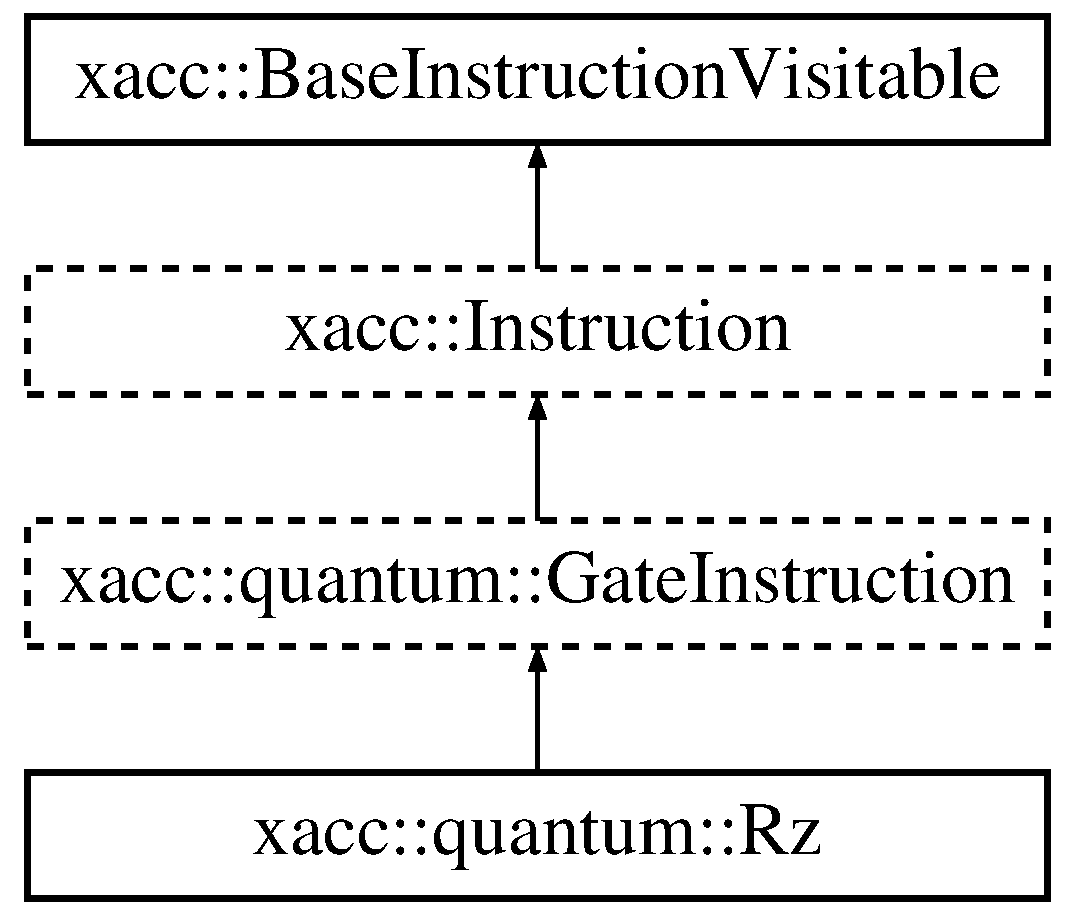
\includegraphics[height=3.000000cm]{a00063}
\end{center}
\end{figure}
\subsection*{Public Member Functions}
\begin{DoxyCompactItemize}
\item 
virtual std\+::shared\+\_\+ptr$<$ \hyperlink{a00051}{xacc\+::\+IR} $>$ \hyperlink{a00063_a2421482415ca4e09963ea4ecddff8100}{compile} (const std\+::string \&src, std\+::shared\+\_\+ptr$<$ \hyperlink{a00011}{Accelerator} $>$ acc)
\item 
virtual std\+::shared\+\_\+ptr$<$ \hyperlink{a00051}{xacc\+::\+IR} $>$ \hyperlink{a00063_adf4d321ecb0df3fa7728999f941c83b2}{compile} (const std\+::string \&src)
\item 
virtual const std\+::string \hyperlink{a00063_ae7d52140b6dd52730edc6e38ae48f437}{get\+Name} ()
\item 
virtual const std\+::string \hyperlink{a00063_a66ca00bbb1f30e7bc6dd86b1e267b93b}{translate} (const std\+::string \&buffer\+Variable, std\+::shared\+\_\+ptr$<$ \hyperlink{a00039}{Function} $>$ function)
\item 
virtual \hyperlink{a00063_a0866a9f695f28c90ac1f4754374f3bfe}{$\sim$\+Quil\+Compiler} ()
\end{DoxyCompactItemize}
\subsection*{Static Public Member Functions}
\begin{DoxyCompactItemize}
\item 
static void \hyperlink{a00063_aaec99a14bede717bf02a0f65af2a3c69}{register\+Compiler} ()
\end{DoxyCompactItemize}
\subsection*{Additional Inherited Members}


\subsection{Constructor \& Destructor Documentation}
\index{xacc\+::quantum\+::\+Quil\+Compiler@{xacc\+::quantum\+::\+Quil\+Compiler}!````~Quil\+Compiler@{$\sim$\+Quil\+Compiler}}
\index{````~Quil\+Compiler@{$\sim$\+Quil\+Compiler}!xacc\+::quantum\+::\+Quil\+Compiler@{xacc\+::quantum\+::\+Quil\+Compiler}}
\subsubsection[{\texorpdfstring{$\sim$\+Quil\+Compiler()}{~QuilCompiler()}}]{\setlength{\rightskip}{0pt plus 5cm}virtual xacc\+::quantum\+::\+Quil\+Compiler\+::$\sim$\+Quil\+Compiler (
\begin{DoxyParamCaption}
{}
\end{DoxyParamCaption}
)\hspace{0.3cm}{\ttfamily [inline]}, {\ttfamily [virtual]}}\hypertarget{a00063_a0866a9f695f28c90ac1f4754374f3bfe}{}\label{a00063_a0866a9f695f28c90ac1f4754374f3bfe}
The destructor 

\subsection{Member Function Documentation}
\index{xacc\+::quantum\+::\+Quil\+Compiler@{xacc\+::quantum\+::\+Quil\+Compiler}!compile@{compile}}
\index{compile@{compile}!xacc\+::quantum\+::\+Quil\+Compiler@{xacc\+::quantum\+::\+Quil\+Compiler}}
\subsubsection[{\texorpdfstring{compile(const std\+::string \&src, std\+::shared\+\_\+ptr$<$ Accelerator $>$ acc)}{compile(const std::string \&src, std::shared\_ptr< Accelerator > acc)}}]{\setlength{\rightskip}{0pt plus 5cm}std\+::shared\+\_\+ptr$<$ {\bf IR} $>$ xacc\+::quantum\+::\+Quil\+Compiler\+::compile (
\begin{DoxyParamCaption}
\item[{const std\+::string \&}]{src, }
\item[{std\+::shared\+\_\+ptr$<$ {\bf Accelerator} $>$}]{acc}
\end{DoxyParamCaption}
)\hspace{0.3cm}{\ttfamily [virtual]}}\hypertarget{a00063_a2421482415ca4e09963ea4ecddff8100}{}\label{a00063_a2421482415ca4e09963ea4ecddff8100}
Translate Quil to the X\+A\+CC intermediate representation.

\begin{DoxyReturn}{Returns}
ir X\+A\+CC intermediate representation 
\end{DoxyReturn}


Implements \hyperlink{a00023_a546a40c95bb93af6a0c0ac48dbeaffc8}{xacc\+::\+Compiler}.

\index{xacc\+::quantum\+::\+Quil\+Compiler@{xacc\+::quantum\+::\+Quil\+Compiler}!compile@{compile}}
\index{compile@{compile}!xacc\+::quantum\+::\+Quil\+Compiler@{xacc\+::quantum\+::\+Quil\+Compiler}}
\subsubsection[{\texorpdfstring{compile(const std\+::string \&src)}{compile(const std::string \&src)}}]{\setlength{\rightskip}{0pt plus 5cm}std\+::shared\+\_\+ptr$<$ {\bf IR} $>$ xacc\+::quantum\+::\+Quil\+Compiler\+::compile (
\begin{DoxyParamCaption}
\item[{const std\+::string \&}]{src}
\end{DoxyParamCaption}
)\hspace{0.3cm}{\ttfamily [virtual]}}\hypertarget{a00063_adf4d321ecb0df3fa7728999f941c83b2}{}\label{a00063_adf4d321ecb0df3fa7728999f941c83b2}

\begin{DoxyParams}{Parameters}
{\em src} & \\
\hline
\end{DoxyParams}
\begin{DoxyReturn}{Returns}

\end{DoxyReturn}


Implements \hyperlink{a00023_a9092f5f779b570c91569b59621280c04}{xacc\+::\+Compiler}.

\index{xacc\+::quantum\+::\+Quil\+Compiler@{xacc\+::quantum\+::\+Quil\+Compiler}!get\+Name@{get\+Name}}
\index{get\+Name@{get\+Name}!xacc\+::quantum\+::\+Quil\+Compiler@{xacc\+::quantum\+::\+Quil\+Compiler}}
\subsubsection[{\texorpdfstring{get\+Name()}{getName()}}]{\setlength{\rightskip}{0pt plus 5cm}virtual const std\+::string xacc\+::quantum\+::\+Quil\+Compiler\+::get\+Name (
\begin{DoxyParamCaption}
{}
\end{DoxyParamCaption}
)\hspace{0.3cm}{\ttfamily [inline]}, {\ttfamily [virtual]}}\hypertarget{a00063_ae7d52140b6dd52730edc6e38ae48f437}{}\label{a00063_ae7d52140b6dd52730edc6e38ae48f437}
Return the name of this \hyperlink{a00023}{Compiler} \begin{DoxyReturn}{Returns}
name \hyperlink{a00023}{Compiler} name 
\end{DoxyReturn}


Implements \hyperlink{a00023_a87fca9100e6462122f5b687c3a0fb3fb}{xacc\+::\+Compiler}.

\index{xacc\+::quantum\+::\+Quil\+Compiler@{xacc\+::quantum\+::\+Quil\+Compiler}!register\+Compiler@{register\+Compiler}}
\index{register\+Compiler@{register\+Compiler}!xacc\+::quantum\+::\+Quil\+Compiler@{xacc\+::quantum\+::\+Quil\+Compiler}}
\subsubsection[{\texorpdfstring{register\+Compiler()}{registerCompiler()}}]{\setlength{\rightskip}{0pt plus 5cm}static void xacc\+::quantum\+::\+Quil\+Compiler\+::register\+Compiler (
\begin{DoxyParamCaption}
{}
\end{DoxyParamCaption}
)\hspace{0.3cm}{\ttfamily [inline]}, {\ttfamily [static]}}\hypertarget{a00063_aaec99a14bede717bf02a0f65af2a3c69}{}\label{a00063_aaec99a14bede717bf02a0f65af2a3c69}
Register this \hyperlink{a00023}{Compiler} with the framework. \index{xacc\+::quantum\+::\+Quil\+Compiler@{xacc\+::quantum\+::\+Quil\+Compiler}!translate@{translate}}
\index{translate@{translate}!xacc\+::quantum\+::\+Quil\+Compiler@{xacc\+::quantum\+::\+Quil\+Compiler}}
\subsubsection[{\texorpdfstring{translate(const std\+::string \&buffer\+Variable, std\+::shared\+\_\+ptr$<$ Function $>$ function)}{translate(const std::string \&bufferVariable, std::shared\_ptr< Function > function)}}]{\setlength{\rightskip}{0pt plus 5cm}const std\+::string xacc\+::quantum\+::\+Quil\+Compiler\+::translate (
\begin{DoxyParamCaption}
\item[{const std\+::string \&}]{buffer\+Variable, }
\item[{std\+::shared\+\_\+ptr$<$ {\bf Function} $>$}]{function}
\end{DoxyParamCaption}
)\hspace{0.3cm}{\ttfamily [virtual]}}\hypertarget{a00063_a66ca00bbb1f30e7bc6dd86b1e267b93b}{}\label{a00063_a66ca00bbb1f30e7bc6dd86b1e267b93b}
This produces a Quil source code representation of the given \hyperlink{a00051}{IR} \hyperlink{a00039}{Function}


\begin{DoxyParams}{Parameters}
{\em function} & The X\+A\+CC \hyperlink{a00051}{IR} \hyperlink{a00039}{Function} to translate \\
\hline
\end{DoxyParams}
\begin{DoxyReturn}{Returns}
src The source code as a string 
\end{DoxyReturn}


Implements \hyperlink{a00023_aeedbe58a33fed29e4d7694ae743e25e7}{xacc\+::\+Compiler}.



The documentation for this class was generated from the following files\+:\begin{DoxyCompactItemize}
\item 
Quil\+Compiler.\+hpp\item 
Quil\+Compiler.\+cpp\end{DoxyCompactItemize}

\hypertarget{a00064}{}\section{boost\+:\+:dll\+:\+:detail\+:\+:constructor$<$ Class(Args...)$>$ Struct Template Reference}
\label{a00064}\index{boost\+::dll\+::detail\+::constructor$<$ Class(\+Args...)$>$@{boost\+::dll\+::detail\+::constructor$<$ Class(\+Args...)$>$}}
\subsection*{Public Types}
\begin{DoxyCompactItemize}
\item 
typedef \hyperlink{a00131}{detail\+::get\+\_\+mem\+\_\+fn\+\_\+type}$<$ Class, void(Args...)$>$\+::mem\+\_\+fn {\bfseries standard\+\_\+t}\hypertarget{a00064_ab765d8c7c083efce92a933c806a41e81}{}\label{a00064_ab765d8c7c083efce92a933c806a41e81}

\item 
typedef Class $\ast$($\ast$ {\bfseries allocating\+\_\+t}) (Args...)\hypertarget{a00064_a19159ea77e5c102bd216195b32045677}{}\label{a00064_a19159ea77e5c102bd216195b32045677}

\end{DoxyCompactItemize}
\subsection*{Public Member Functions}
\begin{DoxyCompactItemize}
\item 
void \hyperlink{a00064_a2b0dbd4b6c5fb1c8fa284b64f85e3caa}{call\+\_\+standard} (Class $\ast$const ptr, Args...\+args)\hypertarget{a00064_a2b0dbd4b6c5fb1c8fa284b64f85e3caa}{}\label{a00064_a2b0dbd4b6c5fb1c8fa284b64f85e3caa}

\begin{DoxyCompactList}\small\item\em Call the standard contructor. \end{DoxyCompactList}\item 
Class $\ast$ \hyperlink{a00064_a9674344355e9759b8f60a4eb92e718af}{call\+\_\+allocating} (Args...\+args)\hypertarget{a00064_a9674344355e9759b8f60a4eb92e718af}{}\label{a00064_a9674344355e9759b8f60a4eb92e718af}

\begin{DoxyCompactList}\small\item\em Call the deleting destructor. \end{DoxyCompactList}\item 
bool \hyperlink{a00064_a2bb649c5d51e8ae9656db16b65776f1c}{has\+\_\+allocating} () const \hypertarget{a00064_a2bb649c5d51e8ae9656db16b65776f1c}{}\label{a00064_a2bb649c5d51e8ae9656db16b65776f1c}

\begin{DoxyCompactList}\small\item\em True if a allocating constructor could be loaded. \end{DoxyCompactList}\item 
bool \hyperlink{a00064_a383752514de8d2f1ffdd142f642e54a3}{has\+\_\+standard} () const \hypertarget{a00064_a383752514de8d2f1ffdd142f642e54a3}{}\label{a00064_a383752514de8d2f1ffdd142f642e54a3}

\begin{DoxyCompactList}\small\item\em True if a standard constructor could be loaded. \end{DoxyCompactList}\item 
bool \hyperlink{a00064_af65e82bd30161ccf3ea05f87193c3fa1}{is\+\_\+empty} () const \hypertarget{a00064_af65e82bd30161ccf3ea05f87193c3fa1}{}\label{a00064_af65e82bd30161ccf3ea05f87193c3fa1}

\begin{DoxyCompactList}\small\item\em False if neither the allocating nor the standard constructor is available. \end{DoxyCompactList}\item 
{\bfseries constructor} (const \hyperlink{a00063}{constructor} \&)=default\hypertarget{a00064_a6ae77617757558a1b0177d6a2cae9827}{}\label{a00064_a6ae77617757558a1b0177d6a2cae9827}

\item 
{\bfseries constructor} (standard\+\_\+t \hyperlink{a00064_a6cbccda8c81959e8e3bba7da28cada5d}{standard}, allocating\+\_\+t \hyperlink{a00064_a13c90a276dc453ca83da117ffc552362}{allocating}=nullptr)\hypertarget{a00064_a403d27f9f509c0ce4e66d4713ca2affc}{}\label{a00064_a403d27f9f509c0ce4e66d4713ca2affc}

\end{DoxyCompactItemize}
\subsection*{Public Attributes}
\begin{DoxyCompactItemize}
\item 
standard\+\_\+t \hyperlink{a00064_a6cbccda8c81959e8e3bba7da28cada5d}{standard}
\begin{DoxyCompactList}\small\item\em The standard, i.\+e. not allocating constructor. \end{DoxyCompactList}\item 
allocating\+\_\+t \hyperlink{a00064_a13c90a276dc453ca83da117ffc552362}{allocating}
\begin{DoxyCompactList}\small\item\em The allocating constructor. \end{DoxyCompactList}\end{DoxyCompactItemize}


\subsection{Member Data Documentation}
\index{boost\+::dll\+::detail\+::constructor$<$ Class(\+Args...)$>$@{boost\+::dll\+::detail\+::constructor$<$ Class(\+Args...)$>$}!allocating@{allocating}}
\index{allocating@{allocating}!boost\+::dll\+::detail\+::constructor$<$ Class(\+Args...)$>$@{boost\+::dll\+::detail\+::constructor$<$ Class(\+Args...)$>$}}
\subsubsection[{\texorpdfstring{allocating}{allocating}}]{\setlength{\rightskip}{0pt plus 5cm}template$<$typename Class , typename... Args$>$ allocating\+\_\+t {\bf boost\+::dll\+::detail\+::constructor}$<$ Class(Args...)$>$\+::allocating}\hypertarget{a00064_a13c90a276dc453ca83da117ffc552362}{}\label{a00064_a13c90a276dc453ca83da117ffc552362}


The allocating constructor. 

\begin{DoxyWarning}{Warning}
May differ with the compiler. Use constructor\+::call\+\_\+allocating instead. 
\end{DoxyWarning}
\index{boost\+::dll\+::detail\+::constructor$<$ Class(\+Args...)$>$@{boost\+::dll\+::detail\+::constructor$<$ Class(\+Args...)$>$}!standard@{standard}}
\index{standard@{standard}!boost\+::dll\+::detail\+::constructor$<$ Class(\+Args...)$>$@{boost\+::dll\+::detail\+::constructor$<$ Class(\+Args...)$>$}}
\subsubsection[{\texorpdfstring{standard}{standard}}]{\setlength{\rightskip}{0pt plus 5cm}template$<$typename Class , typename... Args$>$ standard\+\_\+t {\bf boost\+::dll\+::detail\+::constructor}$<$ Class(Args...)$>$\+::standard}\hypertarget{a00064_a6cbccda8c81959e8e3bba7da28cada5d}{}\label{a00064_a6cbccda8c81959e8e3bba7da28cada5d}


The standard, i.\+e. not allocating constructor. 

\begin{DoxyWarning}{Warning}
May differ with the compiler. Use constructor\+::call\+\_\+standard instead. 
\end{DoxyWarning}


The documentation for this struct was generated from the following file\+:\begin{DoxyCompactItemize}
\item 
ctor\+\_\+dtor.\+hpp\end{DoxyCompactItemize}

\hypertarget{a00065}{}\section{xacc\+:\+:Register\+Algorithm\+Generator$<$ T $>$ Class Template Reference}
\label{a00065}\index{xacc\+::\+Register\+Algorithm\+Generator$<$ T $>$@{xacc\+::\+Register\+Algorithm\+Generator$<$ T $>$}}


{\ttfamily \#include $<$Algorithm\+Generator.\+hpp$>$}

\subsection*{Public Member Functions}
\begin{DoxyCompactItemize}
\item 
{\bfseries Register\+Algorithm\+Generator} (const std\+::string \&name)\hypertarget{a00065_af439cc4d7c8d6628a979129a5c1411df}{}\label{a00065_af439cc4d7c8d6628a979129a5c1411df}

\end{DoxyCompactItemize}


\subsection{Detailed Description}
\subsubsection*{template$<$typename T$>$\\*
class xacc\+::\+Register\+Algorithm\+Generator$<$ T $>$}

\hyperlink{a00065}{Register\+Algorithm\+Generator} is a convenience class for registering custom derived \hyperlink{a00014}{Algorithm\+Generator} classes.

Creators of \hyperlink{a00014}{Algorithm\+Generator} subclasses create an instance of this class with their \hyperlink{a00014}{Algorithm\+Generator} subclass as the template parameter to register their \hyperlink{a00014}{Algorithm\+Generator} with X\+A\+CC. This instance must be created in the C\+PP implementation file for the \hyperlink{a00014}{Algorithm\+Generator} and at global scope. 

The documentation for this class was generated from the following file\+:\begin{DoxyCompactItemize}
\item 
Algorithm\+Generator.\+hpp\end{DoxyCompactItemize}

\hypertarget{a00066}{}\section{xacc\+:\+:Register\+Compiler$<$ T $>$ Class Template Reference}
\label{a00066}\index{xacc\+::\+Register\+Compiler$<$ T $>$@{xacc\+::\+Register\+Compiler$<$ T $>$}}


{\ttfamily \#include $<$Compiler.\+hpp$>$}

\subsection*{Public Member Functions}
\begin{DoxyCompactItemize}
\item 
{\bfseries Register\+Compiler} (const std\+::string \&name)\hypertarget{a00066_a41f5c1abd570b3867b9790cdc02f3355}{}\label{a00066_a41f5c1abd570b3867b9790cdc02f3355}

\item 
{\bfseries Register\+Compiler} (const std\+::string \&name, std\+::shared\+\_\+ptr$<$ options\+\_\+description $>$ options)\hypertarget{a00066_a3489e8cf59f2b0c14e4e2037b61bc368}{}\label{a00066_a3489e8cf59f2b0c14e4e2037b61bc368}

\end{DoxyCompactItemize}


\subsection{Detailed Description}
\subsubsection*{template$<$typename T$>$\\*
class xacc\+::\+Register\+Compiler$<$ T $>$}

\hyperlink{a00066}{Register\+Compiler} is a convenience class for registering custom derived \hyperlink{a00023}{Compiler} classes.

Creators of \hyperlink{a00023}{Compiler} subclasses create an instance of this class with their \hyperlink{a00023}{Compiler} subclass as the template parameter to register their \hyperlink{a00023}{Compiler} with X\+A\+CC. This instance must be created in the C\+PP implementation file for the \hyperlink{a00023}{Compiler} and at global scope. 

The documentation for this class was generated from the following file\+:\begin{DoxyCompactItemize}
\item 
Compiler.\+hpp\end{DoxyCompactItemize}

\hypertarget{a00067}{}\section{xacc\+:\+:quantum\+:\+:Simulated\+Qubits$<$ Total\+Number\+Of\+Qubits $>$ Class Template Reference}
\label{a00067}\index{xacc\+::quantum\+::\+Simulated\+Qubits$<$ Total\+Number\+Of\+Qubits $>$@{xacc\+::quantum\+::\+Simulated\+Qubits$<$ Total\+Number\+Of\+Qubits $>$}}


{\ttfamily \#include $<$Simulated\+Qubits.\+hpp$>$}

Inheritance diagram for xacc\+:\+:quantum\+:\+:Simulated\+Qubits$<$ Total\+Number\+Of\+Qubits $>$\+:\begin{figure}[H]
\begin{center}
\leavevmode
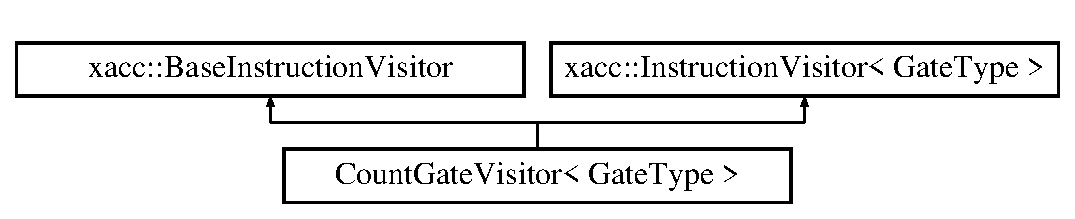
\includegraphics[height=2.000000cm]{a00067}
\end{center}
\end{figure}
\subsection*{Public Member Functions}
\begin{DoxyCompactItemize}
\item 
\hyperlink{a00067_afeb610fbd0c761caa15136e77260ba48}{Simulated\+Qubits} (const std\+::string \&str)
\item 
\hyperlink{a00067_a3d0f465d821565c582c37b6b4d7e4f79}{Simulated\+Qubits} (const std\+::string \&str, const int N)
\item 
{\footnotesize template$<$typename... Indices$>$ }\\{\bfseries Simulated\+Qubits} (const std\+::string \&str, int first\+Index, Indices...\+indices)\hypertarget{a00067_a9366eb77384fb1e9f34a693b9a7ea1b8}{}\label{a00067_a9366eb77384fb1e9f34a693b9a7ea1b8}

\item 
void \hyperlink{a00067_a97ecaaf5aab14bc017726fe9cfd41c46}{apply\+Unitary} (fire\+::\+Tensor$<$ 2, fire\+::\+Eigen\+Provider, std\+::complex$<$ double $>$$>$ \&U)
\item 
void \hyperlink{a00067_aea8a0358100e815a7c70eee7f8ba9d45}{normalize} ()
\item 
Qubit\+State \& \hyperlink{a00067_a75b8fde8e812931fe087cb078108c00d}{get\+State} ()
\item 
void \hyperlink{a00067_a2a0e202f943d3ec8d848c7e25062c6e1}{set\+State} (Qubit\+State \&st)
\item 
virtual bool \hyperlink{a00067_ac689b60b0218bf8d0c11ef2f151e7272}{is\+Valid\+Buffer\+Size} (const int N)
\item 
virtual void \hyperlink{a00067_ad9a39b44161fa0309167b9791ed10945}{print} (std\+::ostream \&stream)
\item 
virtual void {\bfseries print} ()\hypertarget{a00067_a7cda9427b5a0d3eaa9573eb9d992f51c}{}\label{a00067_a7cda9427b5a0d3eaa9573eb9d992f51c}

\end{DoxyCompactItemize}
\subsection*{Protected Attributes}
\begin{DoxyCompactItemize}
\item 
Qubit\+State \hyperlink{a00067_ade9f334823890b3c0553800188ac3ef9}{buffer\+State}
\end{DoxyCompactItemize}


\subsection{Detailed Description}
\subsubsection*{template$<$const int Total\+Number\+Of\+Qubits$>$\\*
class xacc\+::quantum\+::\+Simulated\+Qubits$<$ Total\+Number\+Of\+Qubits $>$}

\hyperlink{a00067}{Simulated\+Qubits} is an \hyperlink{a00013}{Accelerator\+Buffer} that models simulated qubits. As such, it keeps track of the state of the qubit buffer using a Rank 1 Fire Tensor.

It provides an interface for applying unitary operations on the qubit buffer state. 

\subsection{Constructor \& Destructor Documentation}
\index{xacc\+::quantum\+::\+Simulated\+Qubits@{xacc\+::quantum\+::\+Simulated\+Qubits}!Simulated\+Qubits@{Simulated\+Qubits}}
\index{Simulated\+Qubits@{Simulated\+Qubits}!xacc\+::quantum\+::\+Simulated\+Qubits@{xacc\+::quantum\+::\+Simulated\+Qubits}}
\subsubsection[{\texorpdfstring{Simulated\+Qubits(const std\+::string \&str)}{SimulatedQubits(const std::string \&str)}}]{\setlength{\rightskip}{0pt plus 5cm}template$<$const int Total\+Number\+Of\+Qubits$>$ {\bf xacc\+::quantum\+::\+Simulated\+Qubits}$<$ Total\+Number\+Of\+Qubits $>$\+::{\bf Simulated\+Qubits} (
\begin{DoxyParamCaption}
\item[{const std\+::string \&}]{str}
\end{DoxyParamCaption}
)\hspace{0.3cm}{\ttfamily [inline]}}\hypertarget{a00067_afeb610fbd0c761caa15136e77260ba48}{}\label{a00067_afeb610fbd0c761caa15136e77260ba48}
The Constructor, creates a state of size 2$^\wedge$\+Total\+Number\+Of\+Qubits.


\begin{DoxyParams}{Parameters}
{\em str} & \\
\hline
\end{DoxyParams}
\index{xacc\+::quantum\+::\+Simulated\+Qubits@{xacc\+::quantum\+::\+Simulated\+Qubits}!Simulated\+Qubits@{Simulated\+Qubits}}
\index{Simulated\+Qubits@{Simulated\+Qubits}!xacc\+::quantum\+::\+Simulated\+Qubits@{xacc\+::quantum\+::\+Simulated\+Qubits}}
\subsubsection[{\texorpdfstring{Simulated\+Qubits(const std\+::string \&str, const int N)}{SimulatedQubits(const std::string \&str, const int N)}}]{\setlength{\rightskip}{0pt plus 5cm}template$<$const int Total\+Number\+Of\+Qubits$>$ {\bf xacc\+::quantum\+::\+Simulated\+Qubits}$<$ Total\+Number\+Of\+Qubits $>$\+::{\bf Simulated\+Qubits} (
\begin{DoxyParamCaption}
\item[{const std\+::string \&}]{str, }
\item[{const int}]{N}
\end{DoxyParamCaption}
)\hspace{0.3cm}{\ttfamily [inline]}}\hypertarget{a00067_a3d0f465d821565c582c37b6b4d7e4f79}{}\label{a00067_a3d0f465d821565c582c37b6b4d7e4f79}
The Constructor, creates a state with given size N. 
\begin{DoxyParams}{Parameters}
{\em str} & \\
\hline
{\em N} & \\
\hline
\end{DoxyParams}


\subsection{Member Function Documentation}
\index{xacc\+::quantum\+::\+Simulated\+Qubits@{xacc\+::quantum\+::\+Simulated\+Qubits}!apply\+Unitary@{apply\+Unitary}}
\index{apply\+Unitary@{apply\+Unitary}!xacc\+::quantum\+::\+Simulated\+Qubits@{xacc\+::quantum\+::\+Simulated\+Qubits}}
\subsubsection[{\texorpdfstring{apply\+Unitary(fire\+::\+Tensor$<$ 2, fire\+::\+Eigen\+Provider, std\+::complex$<$ double $>$$>$ \&\+U)}{applyUnitary(fire::Tensor< 2, fire::EigenProvider, std::complex< double >> \&U)}}]{\setlength{\rightskip}{0pt plus 5cm}template$<$const int Total\+Number\+Of\+Qubits$>$ void {\bf xacc\+::quantum\+::\+Simulated\+Qubits}$<$ Total\+Number\+Of\+Qubits $>$\+::apply\+Unitary (
\begin{DoxyParamCaption}
\item[{fire\+::\+Tensor$<$ 2, fire\+::\+Eigen\+Provider, std\+::complex$<$ double $>$$>$ \&}]{U}
\end{DoxyParamCaption}
)\hspace{0.3cm}{\ttfamily [inline]}}\hypertarget{a00067_a97ecaaf5aab14bc017726fe9cfd41c46}{}\label{a00067_a97ecaaf5aab14bc017726fe9cfd41c46}
Apply the given unitary matrix to this qubit buffer state.


\begin{DoxyParams}{Parameters}
{\em U} & \\
\hline
\end{DoxyParams}
\index{xacc\+::quantum\+::\+Simulated\+Qubits@{xacc\+::quantum\+::\+Simulated\+Qubits}!get\+State@{get\+State}}
\index{get\+State@{get\+State}!xacc\+::quantum\+::\+Simulated\+Qubits@{xacc\+::quantum\+::\+Simulated\+Qubits}}
\subsubsection[{\texorpdfstring{get\+State()}{getState()}}]{\setlength{\rightskip}{0pt plus 5cm}template$<$const int Total\+Number\+Of\+Qubits$>$ Qubit\+State\& {\bf xacc\+::quantum\+::\+Simulated\+Qubits}$<$ Total\+Number\+Of\+Qubits $>$\+::get\+State (
\begin{DoxyParamCaption}
{}
\end{DoxyParamCaption}
)\hspace{0.3cm}{\ttfamily [inline]}}\hypertarget{a00067_a75b8fde8e812931fe087cb078108c00d}{}\label{a00067_a75b8fde8e812931fe087cb078108c00d}
Return the current state

\begin{DoxyReturn}{Returns}

\end{DoxyReturn}
\index{xacc\+::quantum\+::\+Simulated\+Qubits@{xacc\+::quantum\+::\+Simulated\+Qubits}!is\+Valid\+Buffer\+Size@{is\+Valid\+Buffer\+Size}}
\index{is\+Valid\+Buffer\+Size@{is\+Valid\+Buffer\+Size}!xacc\+::quantum\+::\+Simulated\+Qubits@{xacc\+::quantum\+::\+Simulated\+Qubits}}
\subsubsection[{\texorpdfstring{is\+Valid\+Buffer\+Size(const int N)}{isValidBufferSize(const int N)}}]{\setlength{\rightskip}{0pt plus 5cm}template$<$const int Total\+Number\+Of\+Qubits$>$ virtual bool {\bf xacc\+::quantum\+::\+Simulated\+Qubits}$<$ Total\+Number\+Of\+Qubits $>$\+::is\+Valid\+Buffer\+Size (
\begin{DoxyParamCaption}
\item[{const int}]{N}
\end{DoxyParamCaption}
)\hspace{0.3cm}{\ttfamily [inline]}, {\ttfamily [virtual]}}\hypertarget{a00067_ac689b60b0218bf8d0c11ef2f151e7272}{}\label{a00067_ac689b60b0218bf8d0c11ef2f151e7272}
Allocating this buffer type is only valid if N $<$= Total\+Number\+Of\+Qubits. 
\begin{DoxyParams}{Parameters}
{\em N} & \\
\hline
\end{DoxyParams}
\begin{DoxyReturn}{Returns}

\end{DoxyReturn}
\index{xacc\+::quantum\+::\+Simulated\+Qubits@{xacc\+::quantum\+::\+Simulated\+Qubits}!normalize@{normalize}}
\index{normalize@{normalize}!xacc\+::quantum\+::\+Simulated\+Qubits@{xacc\+::quantum\+::\+Simulated\+Qubits}}
\subsubsection[{\texorpdfstring{normalize()}{normalize()}}]{\setlength{\rightskip}{0pt plus 5cm}template$<$const int Total\+Number\+Of\+Qubits$>$ void {\bf xacc\+::quantum\+::\+Simulated\+Qubits}$<$ Total\+Number\+Of\+Qubits $>$\+::normalize (
\begin{DoxyParamCaption}
{}
\end{DoxyParamCaption}
)\hspace{0.3cm}{\ttfamily [inline]}}\hypertarget{a00067_aea8a0358100e815a7c70eee7f8ba9d45}{}\label{a00067_aea8a0358100e815a7c70eee7f8ba9d45}
Normalize the state. \index{xacc\+::quantum\+::\+Simulated\+Qubits@{xacc\+::quantum\+::\+Simulated\+Qubits}!print@{print}}
\index{print@{print}!xacc\+::quantum\+::\+Simulated\+Qubits@{xacc\+::quantum\+::\+Simulated\+Qubits}}
\subsubsection[{\texorpdfstring{print(std\+::ostream \&stream)}{print(std::ostream \&stream)}}]{\setlength{\rightskip}{0pt plus 5cm}template$<$const int Total\+Number\+Of\+Qubits$>$ virtual void {\bf xacc\+::quantum\+::\+Simulated\+Qubits}$<$ Total\+Number\+Of\+Qubits $>$\+::print (
\begin{DoxyParamCaption}
\item[{std\+::ostream \&}]{stream}
\end{DoxyParamCaption}
)\hspace{0.3cm}{\ttfamily [inline]}, {\ttfamily [virtual]}}\hypertarget{a00067_ad9a39b44161fa0309167b9791ed10945}{}\label{a00067_ad9a39b44161fa0309167b9791ed10945}
Print the state to the provided output stream.


\begin{DoxyParams}{Parameters}
{\em stream} & \\
\hline
\end{DoxyParams}


Reimplemented from \hyperlink{a00013}{Accelerator\+Buffer}.

\index{xacc\+::quantum\+::\+Simulated\+Qubits@{xacc\+::quantum\+::\+Simulated\+Qubits}!set\+State@{set\+State}}
\index{set\+State@{set\+State}!xacc\+::quantum\+::\+Simulated\+Qubits@{xacc\+::quantum\+::\+Simulated\+Qubits}}
\subsubsection[{\texorpdfstring{set\+State(\+Qubit\+State \&st)}{setState(QubitState \&st)}}]{\setlength{\rightskip}{0pt plus 5cm}template$<$const int Total\+Number\+Of\+Qubits$>$ void {\bf xacc\+::quantum\+::\+Simulated\+Qubits}$<$ Total\+Number\+Of\+Qubits $>$\+::set\+State (
\begin{DoxyParamCaption}
\item[{Qubit\+State \&}]{st}
\end{DoxyParamCaption}
)\hspace{0.3cm}{\ttfamily [inline]}}\hypertarget{a00067_a2a0e202f943d3ec8d848c7e25062c6e1}{}\label{a00067_a2a0e202f943d3ec8d848c7e25062c6e1}
Set the state. 
\begin{DoxyParams}{Parameters}
{\em st} & \\
\hline
\end{DoxyParams}


\subsection{Member Data Documentation}
\index{xacc\+::quantum\+::\+Simulated\+Qubits@{xacc\+::quantum\+::\+Simulated\+Qubits}!buffer\+State@{buffer\+State}}
\index{buffer\+State@{buffer\+State}!xacc\+::quantum\+::\+Simulated\+Qubits@{xacc\+::quantum\+::\+Simulated\+Qubits}}
\subsubsection[{\texorpdfstring{buffer\+State}{bufferState}}]{\setlength{\rightskip}{0pt plus 5cm}template$<$const int Total\+Number\+Of\+Qubits$>$ Qubit\+State {\bf xacc\+::quantum\+::\+Simulated\+Qubits}$<$ Total\+Number\+Of\+Qubits $>$\+::buffer\+State\hspace{0.3cm}{\ttfamily [protected]}}\hypertarget{a00067_ade9f334823890b3c0553800188ac3ef9}{}\label{a00067_ade9f334823890b3c0553800188ac3ef9}
The qubit buffer state. 

The documentation for this class was generated from the following file\+:\begin{DoxyCompactItemize}
\item 
Simulated\+Qubits.\+hpp\end{DoxyCompactItemize}

\hypertarget{a00068}{}\section{Crt\+Allocator Class Reference}
\label{a00068}\index{Crt\+Allocator@{Crt\+Allocator}}


C-\/runtime library allocator.  




{\ttfamily \#include $<$allocators.\+h$>$}

\subsection*{Public Member Functions}
\begin{DoxyCompactItemize}
\item 
void $\ast$ {\bfseries Malloc} (size\+\_\+t size)\hypertarget{a00068_acd720631f8c094041afa6c7951f0d935}{}\label{a00068_acd720631f8c094041afa6c7951f0d935}

\item 
void $\ast$ {\bfseries Realloc} (void $\ast$original\+Ptr, size\+\_\+t original\+Size, size\+\_\+t new\+Size)\hypertarget{a00068_a646bb6f68afe773a62a22f7f14f83e97}{}\label{a00068_a646bb6f68afe773a62a22f7f14f83e97}

\end{DoxyCompactItemize}
\subsection*{Static Public Member Functions}
\begin{DoxyCompactItemize}
\item 
static void {\bfseries Free} (void $\ast$ptr)\hypertarget{a00068_a5043907058d906dcb1291e9491560373}{}\label{a00068_a5043907058d906dcb1291e9491560373}

\end{DoxyCompactItemize}
\subsection*{Static Public Attributes}
\begin{DoxyCompactItemize}
\item 
static const bool {\bfseries k\+Need\+Free} = true\hypertarget{a00068_ac7df8398c529290f0cd5950d9492f524}{}\label{a00068_ac7df8398c529290f0cd5950d9492f524}

\end{DoxyCompactItemize}


\subsection{Detailed Description}
C-\/runtime library allocator. 

This class is just wrapper for standard C library memory routines. \begin{DoxyNote}{Note}
implements Allocator concept 
\end{DoxyNote}


The documentation for this class was generated from the following file\+:\begin{DoxyCompactItemize}
\item 
allocators.\+h\end{DoxyCompactItemize}

\hypertarget{a00069}{}\section{xacc\+:\+:Register\+Preprocessor$<$ T $>$ Class Template Reference}
\label{a00069}\index{xacc\+::\+Register\+Preprocessor$<$ T $>$@{xacc\+::\+Register\+Preprocessor$<$ T $>$}}


{\ttfamily \#include $<$Preprocessor.\+hpp$>$}

\subsection*{Public Member Functions}
\begin{DoxyCompactItemize}
\item 
{\bfseries Register\+Preprocessor} (const std\+::string \&name)\hypertarget{a00069_a360d5ffa16ef3a96c3bc61fa897ffe3c}{}\label{a00069_a360d5ffa16ef3a96c3bc61fa897ffe3c}

\end{DoxyCompactItemize}


\subsection{Detailed Description}
\subsubsection*{template$<$typename T$>$\\*
class xacc\+::\+Register\+Preprocessor$<$ T $>$}

\hyperlink{a00069}{Register\+Preprocessor} is a convenience class for registering custom derived \hyperlink{a00057}{Preprocessor} classes.

Creators of \hyperlink{a00057}{Preprocessor} subclasses create an instance of this class with their \hyperlink{a00057}{Preprocessor} subclass as the template parameter to register their \hyperlink{a00057}{Preprocessor} with X\+A\+CC. This instance must be created in the C\+PP implementation file for the \hyperlink{a00057}{Preprocessor} and at global scope. 

The documentation for this class was generated from the following file\+:\begin{DoxyCompactItemize}
\item 
Preprocessor.\+hpp\end{DoxyCompactItemize}

\hypertarget{a00070}{}\section{xacc\+:\+:quantum\+:\+:X Class Reference}
\label{a00070}\index{xacc\+::quantum\+::X@{xacc\+::quantum\+::X}}
Inheritance diagram for xacc\+:\+:quantum\+:\+:X\+:\begin{figure}[H]
\begin{center}
\leavevmode
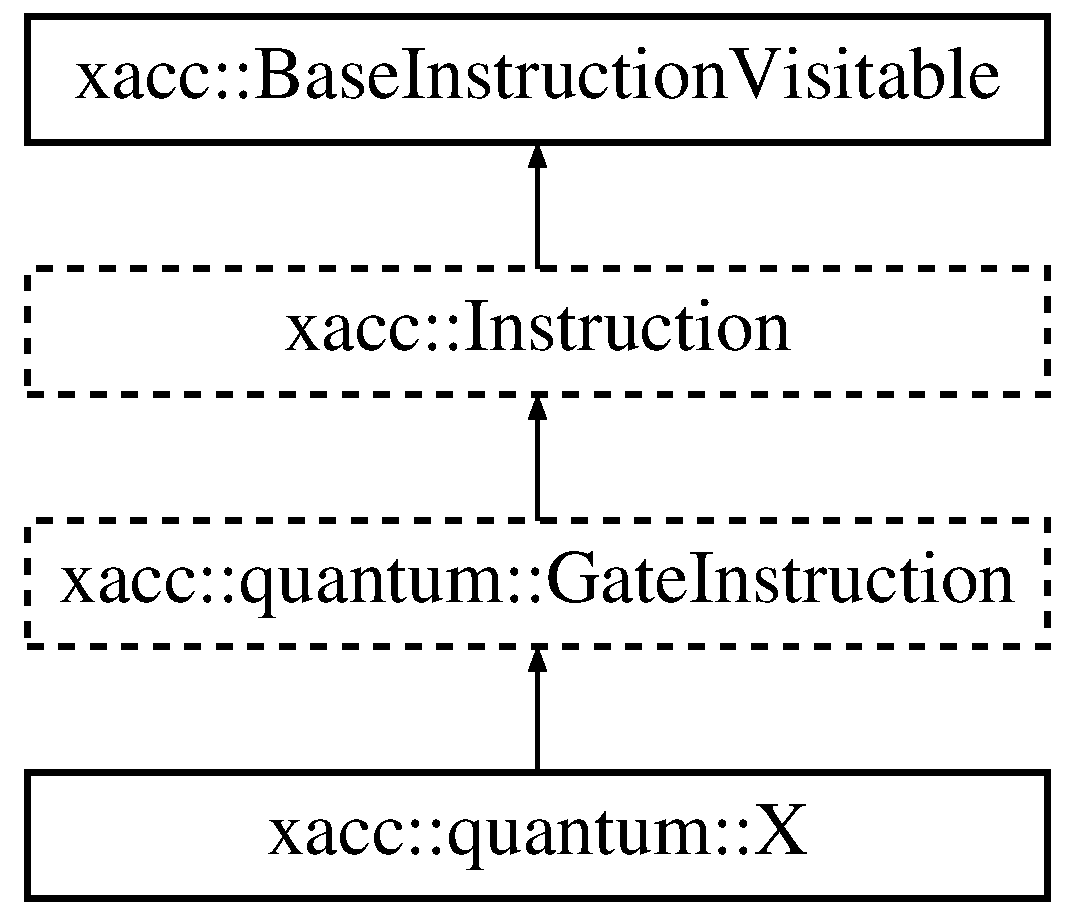
\includegraphics[height=4.000000cm]{a00070}
\end{center}
\end{figure}
\subsection*{Public Member Functions}
\begin{DoxyCompactItemize}
\item 
{\bfseries X} (std\+::vector$<$ int $>$ qbit)\hypertarget{a00070_aedc541a302602154847118f73b040510}{}\label{a00070_aedc541a302602154847118f73b040510}

\item 
{\bfseries X} (int qbit)\hypertarget{a00070_a1159bd01929b59277b4524ccfcfd7440}{}\label{a00070_a1159bd01929b59277b4524ccfcfd7440}

\end{DoxyCompactItemize}
\subsection*{Additional Inherited Members}


The documentation for this class was generated from the following files\+:\begin{DoxyCompactItemize}
\item 
X.\+hpp\item 
X.\+cpp\end{DoxyCompactItemize}

\hypertarget{a00071}{}\section{Generic\+Value$<$ Encoding, Allocator $>$\+:\+:Data Union Reference}
\label{a00071}\index{Generic\+Value$<$ Encoding, Allocator $>$\+::\+Data@{Generic\+Value$<$ Encoding, Allocator $>$\+::\+Data}}
\subsection*{Public Attributes}
\begin{DoxyCompactItemize}
\item 
\hyperlink{a00291}{String} {\bfseries s}\hypertarget{a00071_a6872a4b93763944063b425e6c001ed2b}{}\label{a00071_a6872a4b93763944063b425e6c001ed2b}

\item 
\hyperlink{a00273}{Short\+String} {\bfseries ss}\hypertarget{a00071_a410e39a5dc296eb3b152b54193740e4c}{}\label{a00071_a410e39a5dc296eb3b152b54193740e4c}

\item 
\hyperlink{a00226}{Number} {\bfseries n}\hypertarget{a00071_a243007cce2f4b75bea3e3c1ee4c3c239}{}\label{a00071_a243007cce2f4b75bea3e3c1ee4c3c239}

\item 
\hyperlink{a00227}{Object\+Data} {\bfseries o}\hypertarget{a00071_af6417eca530fba0d8bd65d309628eb11}{}\label{a00071_af6417eca530fba0d8bd65d309628eb11}

\item 
\hyperlink{a00037}{Array\+Data} {\bfseries a}\hypertarget{a00071_aeac31cf55bf5a024cead5ecb63e4fd48}{}\label{a00071_aeac31cf55bf5a024cead5ecb63e4fd48}

\item 
\hyperlink{a00104}{Flag} {\bfseries f}\hypertarget{a00071_ad8572112da083c775ce21bcbca96b2ab}{}\label{a00071_ad8572112da083c775ce21bcbca96b2ab}

\end{DoxyCompactItemize}


The documentation for this union was generated from the following file\+:\begin{DoxyCompactItemize}
\item 
\hyperlink{a00473}{document.\+h}\end{DoxyCompactItemize}

\hypertarget{a00072}{}\section{xacc\+:\+:X\+A\+C\+C\+InfoT Class Reference}
\label{a00072}\index{xacc\+::\+X\+A\+C\+C\+InfoT@{xacc\+::\+X\+A\+C\+C\+InfoT}}
\subsection*{Static Public Member Functions}
\begin{DoxyCompactItemize}
\item 
static void {\bfseries print\+Info} (const std\+::string \&msg)\hypertarget{a00072_afa78299617677d0be1b721600b48a8fa}{}\label{a00072_afa78299617677d0be1b721600b48a8fa}

\end{DoxyCompactItemize}


The documentation for this class was generated from the following file\+:\begin{DoxyCompactItemize}
\item 
Utils.\+hpp\end{DoxyCompactItemize}

\hypertarget{a00073}{}\section{xacc\+:\+:quantum\+:\+:Rx Class Reference}
\label{a00073}\index{xacc\+::quantum\+::\+Rx@{xacc\+::quantum\+::\+Rx}}
Inheritance diagram for xacc\+:\+:quantum\+:\+:Rx\+:\begin{figure}[H]
\begin{center}
\leavevmode
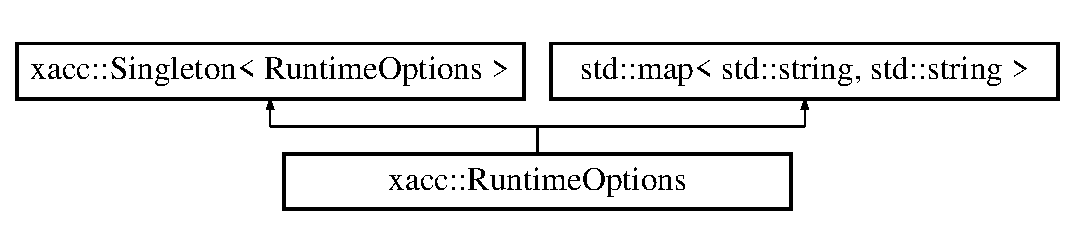
\includegraphics[height=4.000000cm]{a00073}
\end{center}
\end{figure}
\subsection*{Public Member Functions}
\begin{DoxyCompactItemize}
\item 
{\bfseries Rx} (std\+::vector$<$ int $>$ \hyperlink{a00041_a2a56be6c2519ea65df4d06f4abae1393}{qbits})\hypertarget{a00073_a03babfe938a6cbf7f744fcd31a52d92d}{}\label{a00073_a03babfe938a6cbf7f744fcd31a52d92d}

\item 
{\bfseries Rx} (int qbit, double theta)\hypertarget{a00073_a01667b11d34d5621b98ebff9a07d9bbf}{}\label{a00073_a01667b11d34d5621b98ebff9a07d9bbf}

\end{DoxyCompactItemize}
\subsection*{Additional Inherited Members}


The documentation for this class was generated from the following files\+:\begin{DoxyCompactItemize}
\item 
Rx.\+hpp\item 
Rx.\+cpp\end{DoxyCompactItemize}

\hypertarget{a00074}{}\section{xacc\+:\+:quantum\+:\+:Ry Class Reference}
\label{a00074}\index{xacc\+::quantum\+::\+Ry@{xacc\+::quantum\+::\+Ry}}
Inheritance diagram for xacc\+:\+:quantum\+:\+:Ry\+:\begin{figure}[H]
\begin{center}
\leavevmode
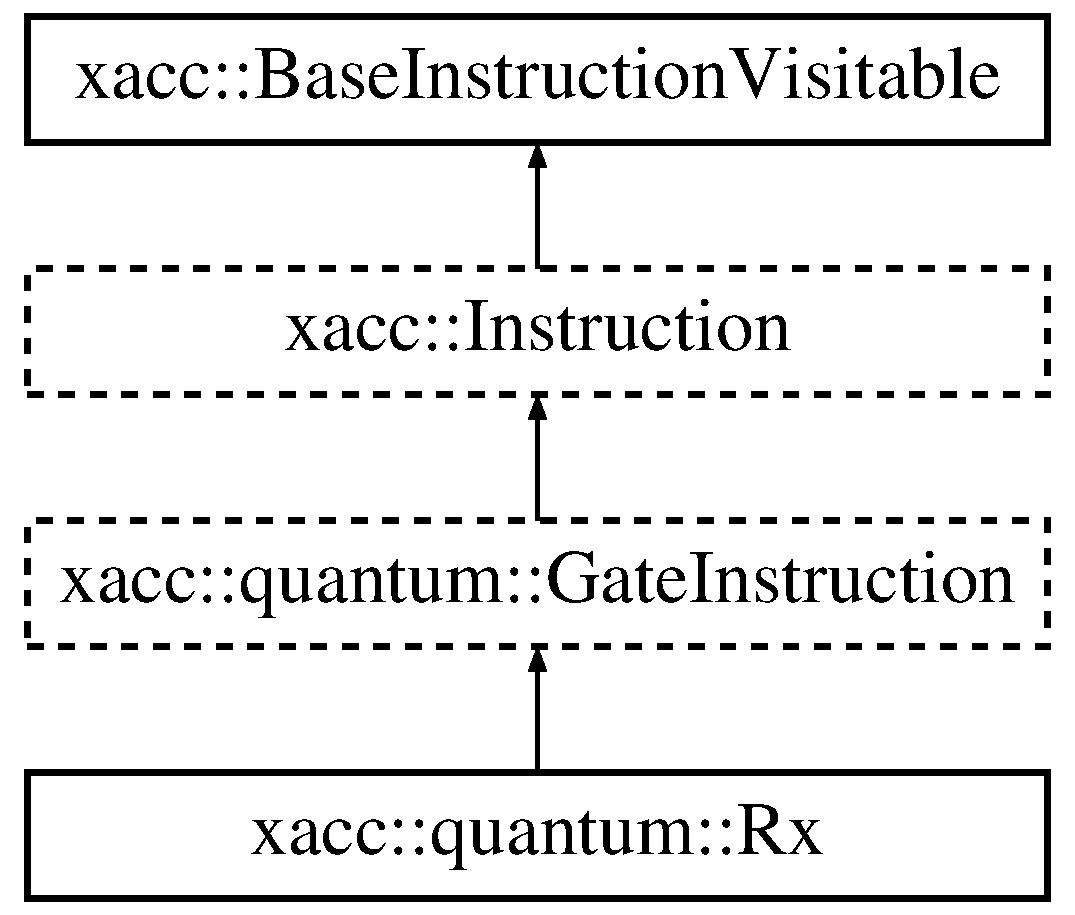
\includegraphics[height=4.000000cm]{a00074}
\end{center}
\end{figure}
\subsection*{Public Member Functions}
\begin{DoxyCompactItemize}
\item 
{\bfseries Ry} (std\+::vector$<$ int $>$ \hyperlink{a00041_a2a56be6c2519ea65df4d06f4abae1393}{qbits})\hypertarget{a00074_a542e1c0576a8e784f6cece4c77598486}{}\label{a00074_a542e1c0576a8e784f6cece4c77598486}

\item 
{\bfseries Ry} (int qbit, double theta)\hypertarget{a00074_a1cb81fe622168ba8d79fa2a78b5b0006}{}\label{a00074_a1cb81fe622168ba8d79fa2a78b5b0006}

\end{DoxyCompactItemize}
\subsection*{Additional Inherited Members}


The documentation for this class was generated from the following files\+:\begin{DoxyCompactItemize}
\item 
Ry.\+hpp\item 
Ry.\+cpp\end{DoxyCompactItemize}

\hypertarget{a00075}{}\section{xacc\+:\+:quantum\+:\+:Inverse\+Q\+FT Class Reference}
\label{a00075}\index{xacc\+::quantum\+::\+Inverse\+Q\+FT@{xacc\+::quantum\+::\+Inverse\+Q\+FT}}


{\ttfamily \#include $<$Inverse\+Q\+F\+T.\+hpp$>$}

Inheritance diagram for xacc\+:\+:quantum\+:\+:Inverse\+Q\+FT\+:\begin{figure}[H]
\begin{center}
\leavevmode
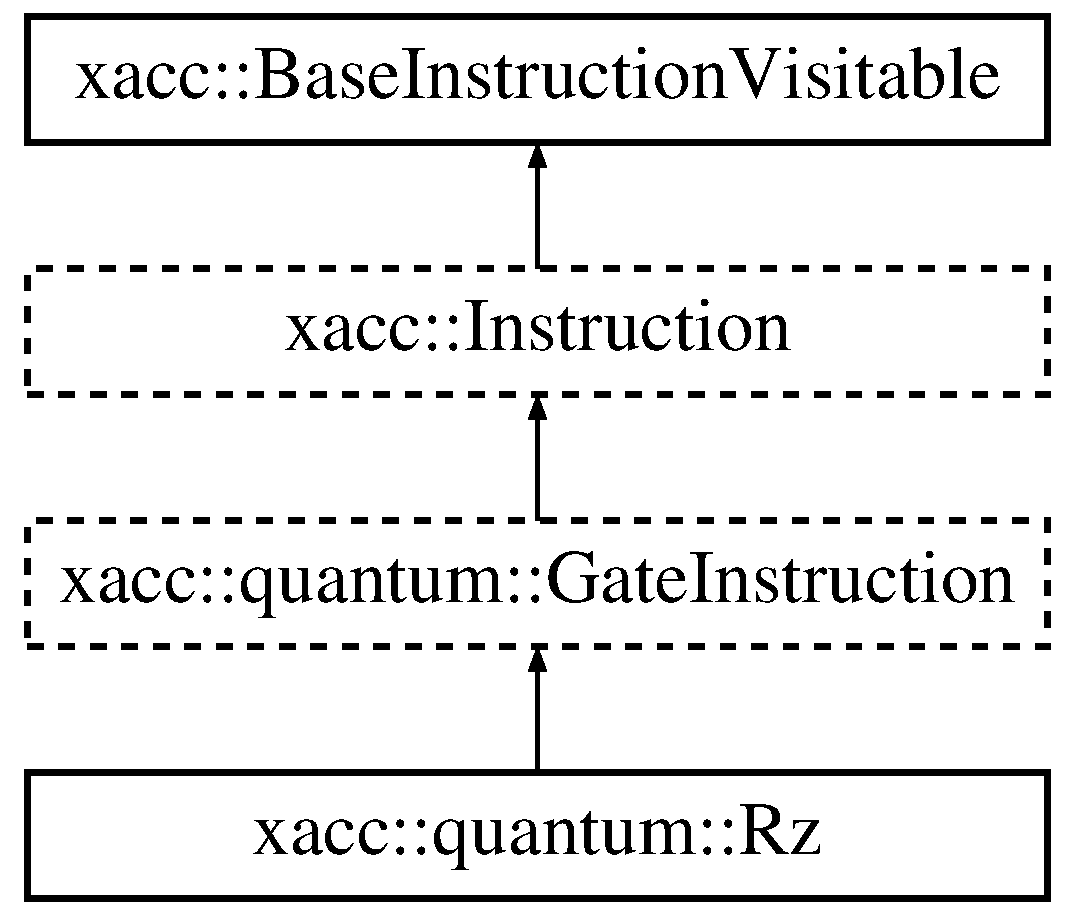
\includegraphics[height=2.000000cm]{a00075}
\end{center}
\end{figure}
\subsection*{Public Member Functions}
\begin{DoxyCompactItemize}
\item 
virtual std\+::shared\+\_\+ptr$<$ \hyperlink{a00059}{Function} $>$ \hyperlink{a00075_af42e466bf02dbd60670d20aa55cfb08d}{generate\+Algorithm} (std\+::vector$<$ int $>$ qubits)
\item 
virtual \hyperlink{a00075_a731c10d28046424be74e4c0daa31d016}{$\sim$\+Inverse\+Q\+FT} ()
\end{DoxyCompactItemize}


\subsection{Detailed Description}
\hyperlink{a00075}{Inverse\+Q\+FT} is a realization of the \hyperlink{a00020}{Algorithm\+Generator} interface that produces an X\+A\+CC \hyperlink{a00077}{IR} representation of the Inverse Quantum Fourier Transform. 

\subsection{Constructor \& Destructor Documentation}
\index{xacc\+::quantum\+::\+Inverse\+Q\+FT@{xacc\+::quantum\+::\+Inverse\+Q\+FT}!````~Inverse\+Q\+FT@{$\sim$\+Inverse\+Q\+FT}}
\index{````~Inverse\+Q\+FT@{$\sim$\+Inverse\+Q\+FT}!xacc\+::quantum\+::\+Inverse\+Q\+FT@{xacc\+::quantum\+::\+Inverse\+Q\+FT}}
\subsubsection[{\texorpdfstring{$\sim$\+Inverse\+Q\+F\+T()}{~InverseQFT()}}]{\setlength{\rightskip}{0pt plus 5cm}virtual xacc\+::quantum\+::\+Inverse\+Q\+F\+T\+::$\sim$\+Inverse\+Q\+FT (
\begin{DoxyParamCaption}
{}
\end{DoxyParamCaption}
)\hspace{0.3cm}{\ttfamily [inline]}, {\ttfamily [virtual]}}\hypertarget{a00075_a731c10d28046424be74e4c0daa31d016}{}\label{a00075_a731c10d28046424be74e4c0daa31d016}
The destructor 

\subsection{Member Function Documentation}
\index{xacc\+::quantum\+::\+Inverse\+Q\+FT@{xacc\+::quantum\+::\+Inverse\+Q\+FT}!generate\+Algorithm@{generate\+Algorithm}}
\index{generate\+Algorithm@{generate\+Algorithm}!xacc\+::quantum\+::\+Inverse\+Q\+FT@{xacc\+::quantum\+::\+Inverse\+Q\+FT}}
\subsubsection[{\texorpdfstring{generate\+Algorithm(std\+::vector$<$ int $>$ qubits)}{generateAlgorithm(std::vector< int > qubits)}}]{\setlength{\rightskip}{0pt plus 5cm}std\+::shared\+\_\+ptr$<$ {\bf Function} $>$ xacc\+::quantum\+::\+Inverse\+Q\+F\+T\+::generate\+Algorithm (
\begin{DoxyParamCaption}
\item[{std\+::vector$<$ int $>$}]{qubits}
\end{DoxyParamCaption}
)\hspace{0.3cm}{\ttfamily [virtual]}}\hypertarget{a00075_af42e466bf02dbd60670d20aa55cfb08d}{}\label{a00075_af42e466bf02dbd60670d20aa55cfb08d}
This implementation returns a \hyperlink{a00059}{Function} \hyperlink{a00077}{IR} representation of the inverse quantum fourier transform.


\begin{DoxyParams}{Parameters}
{\em bits} & The bits this algorithm operates on \\
\hline
\end{DoxyParams}
\begin{DoxyReturn}{Returns}
function The algorithm represented as an \hyperlink{a00077}{IR} \hyperlink{a00059}{Function} 
\end{DoxyReturn}


Implements \hyperlink{a00020_a73023c06f0f0c62ad56ab4187b18b096}{xacc\+::\+Algorithm\+Generator}.



The documentation for this class was generated from the following files\+:\begin{DoxyCompactItemize}
\item 
Inverse\+Q\+F\+T.\+hpp\item 
Inverse\+Q\+F\+T.\+cpp\end{DoxyCompactItemize}

\hypertarget{a00076}{}\section{boost\+:\+:dll\+:\+:detail\+:\+:destructor$<$ Class $>$ Struct Template Reference}
\label{a00076}\index{boost\+::dll\+::detail\+::destructor$<$ Class $>$@{boost\+::dll\+::detail\+::destructor$<$ Class $>$}}
\subsection*{Public Types}
\begin{DoxyCompactItemize}
\item 
typedef void($\ast$ {\bfseries type}) (Class $\ast$const)\hypertarget{a00076_a155dbf742e9c6499f52041d0b9f061be}{}\label{a00076_a155dbf742e9c6499f52041d0b9f061be}

\item 
typedef type {\bfseries standard\+\_\+t}\hypertarget{a00076_a6a72bebfcaef05b746a9b4cf93d66c50}{}\label{a00076_a6a72bebfcaef05b746a9b4cf93d66c50}

\item 
typedef type {\bfseries deleting\+\_\+t}\hypertarget{a00076_aff7ad402a5e8d7c8d1d086f73f3acf88}{}\label{a00076_aff7ad402a5e8d7c8d1d086f73f3acf88}

\end{DoxyCompactItemize}
\subsection*{Public Member Functions}
\begin{DoxyCompactItemize}
\item 
void \hyperlink{a00076_a95d55018849080c7d4c771b564e9b04e}{call\+\_\+standard} (Class $\ast$const ptr)\hypertarget{a00076_a95d55018849080c7d4c771b564e9b04e}{}\label{a00076_a95d55018849080c7d4c771b564e9b04e}

\begin{DoxyCompactList}\small\item\em Call the standard contructor. \end{DoxyCompactList}\item 
void \hyperlink{a00076_aabc107ff82b8a6f7e5aed5bd84080b1f}{call\+\_\+deleting} (Class $\ast$const ptr)\hypertarget{a00076_aabc107ff82b8a6f7e5aed5bd84080b1f}{}\label{a00076_aabc107ff82b8a6f7e5aed5bd84080b1f}

\begin{DoxyCompactList}\small\item\em Call the deleting destructor. \end{DoxyCompactList}\item 
bool \hyperlink{a00076_a294eee52606f8fdfbff528adbc50c3ea}{has\+\_\+deleting} () const \hypertarget{a00076_a294eee52606f8fdfbff528adbc50c3ea}{}\label{a00076_a294eee52606f8fdfbff528adbc50c3ea}

\begin{DoxyCompactList}\small\item\em True if a deleting destructor could be loaded. \end{DoxyCompactList}\item 
bool \hyperlink{a00076_a3efe4b3476a9157740a5a8840ae39186}{has\+\_\+standard} () const \hypertarget{a00076_a3efe4b3476a9157740a5a8840ae39186}{}\label{a00076_a3efe4b3476a9157740a5a8840ae39186}

\begin{DoxyCompactList}\small\item\em True if a standard destructor could be loaded. \end{DoxyCompactList}\item 
bool \hyperlink{a00076_adf4ce5f7e9d65a0ec22abf8109f0a5c3}{is\+\_\+empty} () const \hypertarget{a00076_adf4ce5f7e9d65a0ec22abf8109f0a5c3}{}\label{a00076_adf4ce5f7e9d65a0ec22abf8109f0a5c3}

\begin{DoxyCompactList}\small\item\em False if neither the deleting nor the standard destructor is available. \end{DoxyCompactList}\item 
\hyperlink{a00076_a45248a911612597c871150e12ad3208b}{destructor} (const \hyperlink{a00076}{destructor} \&)=default\hypertarget{a00076_a45248a911612597c871150e12ad3208b}{}\label{a00076_a45248a911612597c871150e12ad3208b}

\begin{DoxyCompactList}\small\item\em Copy destructor. \end{DoxyCompactList}\item 
\hyperlink{a00076_abc1f0cdcc708f43049b7d11727e24f24}{destructor} (const standard\+\_\+t \&\hyperlink{a00076_a5c588780f2142ca3492ea78c62fe472c}{standard}, const deleting\+\_\+t \&\hyperlink{a00076_a96ad279626c7f9b845d47582f9f88dc0}{deleting}=nullptr)\hypertarget{a00076_abc1f0cdcc708f43049b7d11727e24f24}{}\label{a00076_abc1f0cdcc708f43049b7d11727e24f24}

\begin{DoxyCompactList}\small\item\em Construct it from both the standard destructor and the allocating destructor. \end{DoxyCompactList}\end{DoxyCompactItemize}
\subsection*{Public Attributes}
\begin{DoxyCompactItemize}
\item 
standard\+\_\+t \hyperlink{a00076_a5c588780f2142ca3492ea78c62fe472c}{standard}
\begin{DoxyCompactList}\small\item\em The standard, i.\+e. not deleting destructor. \end{DoxyCompactList}\item 
deleting\+\_\+t \hyperlink{a00076_a96ad279626c7f9b845d47582f9f88dc0}{deleting}
\begin{DoxyCompactList}\small\item\em The deleting destructor. \end{DoxyCompactList}\end{DoxyCompactItemize}


\subsection{Member Data Documentation}
\index{boost\+::dll\+::detail\+::destructor@{boost\+::dll\+::detail\+::destructor}!deleting@{deleting}}
\index{deleting@{deleting}!boost\+::dll\+::detail\+::destructor@{boost\+::dll\+::detail\+::destructor}}
\subsubsection[{\texorpdfstring{deleting}{deleting}}]{\setlength{\rightskip}{0pt plus 5cm}template$<$typename Class$>$ deleting\+\_\+t {\bf boost\+::dll\+::detail\+::destructor}$<$ Class $>$\+::deleting}\hypertarget{a00076_a96ad279626c7f9b845d47582f9f88dc0}{}\label{a00076_a96ad279626c7f9b845d47582f9f88dc0}


The deleting destructor. 

\begin{DoxyWarning}{Warning}
May differ with the compiler. Use destructor\+::call\+\_\+deallocating instead. 
\end{DoxyWarning}
\index{boost\+::dll\+::detail\+::destructor@{boost\+::dll\+::detail\+::destructor}!standard@{standard}}
\index{standard@{standard}!boost\+::dll\+::detail\+::destructor@{boost\+::dll\+::detail\+::destructor}}
\subsubsection[{\texorpdfstring{standard}{standard}}]{\setlength{\rightskip}{0pt plus 5cm}template$<$typename Class$>$ standard\+\_\+t {\bf boost\+::dll\+::detail\+::destructor}$<$ Class $>$\+::standard}\hypertarget{a00076_a5c588780f2142ca3492ea78c62fe472c}{}\label{a00076_a5c588780f2142ca3492ea78c62fe472c}


The standard, i.\+e. not deleting destructor. 

\begin{DoxyWarning}{Warning}
May differ with the compiler. Use \hyperlink{a00076_a95d55018849080c7d4c771b564e9b04e}{destructor\+::call\+\_\+standard} instead. 
\end{DoxyWarning}


The documentation for this struct was generated from the following file\+:\begin{DoxyCompactItemize}
\item 
ctor\+\_\+dtor.\+hpp\end{DoxyCompactItemize}

\hypertarget{a00077}{}\section{xacc\+:\+:IR Class Reference}
\label{a00077}\index{xacc\+::\+IR@{xacc\+::\+IR}}


{\ttfamily \#include $<$I\+R.\+hpp$>$}

Inheritance diagram for xacc\+:\+:IR\+:\begin{figure}[H]
\begin{center}
\leavevmode
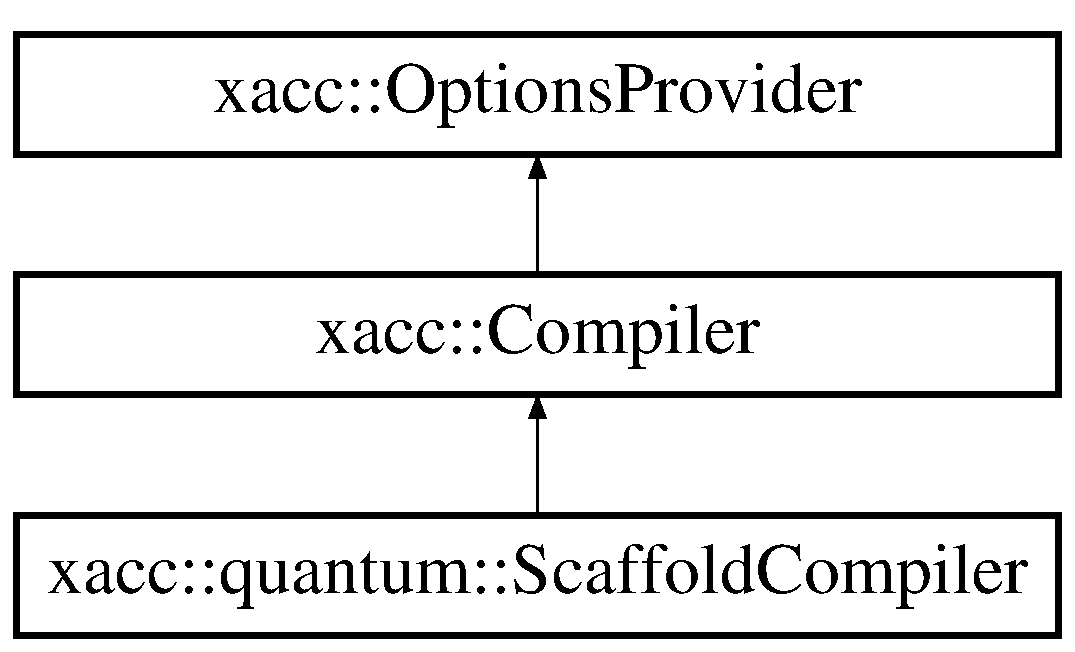
\includegraphics[height=2.000000cm]{a00077}
\end{center}
\end{figure}
\subsection*{Public Member Functions}
\begin{DoxyCompactItemize}
\item 
virtual std\+::string \hyperlink{a00077_a8356cdff1919b88eabeb84fd7450cdb6}{to\+Assembly\+String} (const std\+::string \&kernel\+Name, const std\+::string \&acc\+Buffer\+Var\+Name)=0
\item 
virtual void \hyperlink{a00077_a414b72224d88473ad6190bb88102a3ea}{persist} (std\+::ostream \&out\+Stream)=0
\item 
virtual void \hyperlink{a00077_a444c2e4dc0faac500fb70fa93997e9bc}{load} (std\+::istream \&in\+Stream)=0
\item 
virtual void \hyperlink{a00077_abbbf8e6993c518597de32cd05d49d737}{add\+Kernel} (std\+::shared\+\_\+ptr$<$ \hyperlink{a00059}{Function} $>$ kernel)=0
\item 
virtual bool \hyperlink{a00077_afc9ccf5126f3fed19c2e879133b2f6d8}{kernel\+Exists} (const std\+::string \&name)=0
\item 
virtual std\+::shared\+\_\+ptr$<$ \hyperlink{a00059}{Function} $>$ \hyperlink{a00077_a6f49b4ba4b3a15142b04873284885f0d}{get\+Kernel} (const std\+::string \&name)=0
\item 
virtual std\+::vector$<$ std\+::shared\+\_\+ptr$<$ \hyperlink{a00059}{Function} $>$ $>$ \hyperlink{a00077_a88c50bfc5b279145360ddc0c3a703b9b}{get\+Kernels} ()=0
\item 
virtual \hyperlink{a00077_a09a76d71092254acae07e19fa2f34921}{$\sim$\+IR} ()
\end{DoxyCompactItemize}


\subsection{Detailed Description}
The \hyperlink{a00077}{IR} interface is the base interface for derived accelerator-\/specific intermediate representations. At this level, an intermediate representation can be persisted to an assembly-\/like string, can be read in from file, and can be persisted to file. Since all X\+A\+CC intermediate representations operate on an \hyperlink{a00017}{Accelerator} Buffer, the \hyperlink{a00077}{IR} interface also provides a setter for such a buffer. 

\subsection{Constructor \& Destructor Documentation}
\index{xacc\+::\+IR@{xacc\+::\+IR}!````~IR@{$\sim$\+IR}}
\index{````~IR@{$\sim$\+IR}!xacc\+::\+IR@{xacc\+::\+IR}}
\subsubsection[{\texorpdfstring{$\sim$\+I\+R()}{~IR()}}]{\setlength{\rightskip}{0pt plus 5cm}virtual xacc\+::\+I\+R\+::$\sim$\+IR (
\begin{DoxyParamCaption}
{}
\end{DoxyParamCaption}
)\hspace{0.3cm}{\ttfamily [inline]}, {\ttfamily [virtual]}}\hypertarget{a00077_a09a76d71092254acae07e19fa2f34921}{}\label{a00077_a09a76d71092254acae07e19fa2f34921}
The destructor 

\subsection{Member Function Documentation}
\index{xacc\+::\+IR@{xacc\+::\+IR}!add\+Kernel@{add\+Kernel}}
\index{add\+Kernel@{add\+Kernel}!xacc\+::\+IR@{xacc\+::\+IR}}
\subsubsection[{\texorpdfstring{add\+Kernel(std\+::shared\+\_\+ptr$<$ Function $>$ kernel)=0}{addKernel(std::shared\_ptr< Function > kernel)=0}}]{\setlength{\rightskip}{0pt plus 5cm}virtual void xacc\+::\+I\+R\+::add\+Kernel (
\begin{DoxyParamCaption}
\item[{std\+::shared\+\_\+ptr$<$ {\bf Function} $>$}]{kernel}
\end{DoxyParamCaption}
)\hspace{0.3cm}{\ttfamily [pure virtual]}}\hypertarget{a00077_abbbf8e6993c518597de32cd05d49d737}{}\label{a00077_abbbf8e6993c518597de32cd05d49d737}
Add a new kernel to this \hyperlink{a00077}{IR} instance.


\begin{DoxyParams}{Parameters}
{\em kernel} & The \hyperlink{a00059}{Function} instance to add as a new kernel \\
\hline
\end{DoxyParams}


Implemented in \hyperlink{a00063_aa6ed2cf2cbcfec8105c327a4fa95346f}{xacc\+::quantum\+::\+Gate\+Q\+IR}, and \hyperlink{a00044_af1bef18e1e9568d1313b03149aab8c1b}{xacc\+::quantum\+::\+D\+W\+IR}.

\index{xacc\+::\+IR@{xacc\+::\+IR}!get\+Kernel@{get\+Kernel}}
\index{get\+Kernel@{get\+Kernel}!xacc\+::\+IR@{xacc\+::\+IR}}
\subsubsection[{\texorpdfstring{get\+Kernel(const std\+::string \&name)=0}{getKernel(const std::string \&name)=0}}]{\setlength{\rightskip}{0pt plus 5cm}virtual std\+::shared\+\_\+ptr$<${\bf Function}$>$ xacc\+::\+I\+R\+::get\+Kernel (
\begin{DoxyParamCaption}
\item[{const std\+::string \&}]{name}
\end{DoxyParamCaption}
)\hspace{0.3cm}{\ttfamily [pure virtual]}}\hypertarget{a00077_a6f49b4ba4b3a15142b04873284885f0d}{}\label{a00077_a6f49b4ba4b3a15142b04873284885f0d}
Return the kernel with the given name.


\begin{DoxyParams}{Parameters}
{\em name} & The name of the kernel to return. \\
\hline
\end{DoxyParams}
\begin{DoxyReturn}{Returns}
kernel The kernel with given name. 
\end{DoxyReturn}


Implemented in \hyperlink{a00063_a194758b6edcc3ae0c7fe8004f9bfe690}{xacc\+::quantum\+::\+Gate\+Q\+IR}, and \hyperlink{a00044_a38d8bdd24250749bc38ad31f8512fcfc}{xacc\+::quantum\+::\+D\+W\+IR}.

\index{xacc\+::\+IR@{xacc\+::\+IR}!get\+Kernels@{get\+Kernels}}
\index{get\+Kernels@{get\+Kernels}!xacc\+::\+IR@{xacc\+::\+IR}}
\subsubsection[{\texorpdfstring{get\+Kernels()=0}{getKernels()=0}}]{\setlength{\rightskip}{0pt plus 5cm}virtual std\+::vector$<$std\+::shared\+\_\+ptr$<${\bf Function}$>$ $>$ xacc\+::\+I\+R\+::get\+Kernels (
\begin{DoxyParamCaption}
{}
\end{DoxyParamCaption}
)\hspace{0.3cm}{\ttfamily [pure virtual]}}\hypertarget{a00077_a88c50bfc5b279145360ddc0c3a703b9b}{}\label{a00077_a88c50bfc5b279145360ddc0c3a703b9b}
Return all of this \hyperlink{a00077}{IR} instance\textquotesingle{}s kernels.

\begin{DoxyReturn}{Returns}
kernels The kernels this \hyperlink{a00077}{IR} contains. 
\end{DoxyReturn}


Implemented in \hyperlink{a00063_a4ace7ee5ebef84b1f39aaf5ed12c6cc6}{xacc\+::quantum\+::\+Gate\+Q\+IR}, and \hyperlink{a00044_a66e22c5dc95ec46045476864012ad08f}{xacc\+::quantum\+::\+D\+W\+IR}.

\index{xacc\+::\+IR@{xacc\+::\+IR}!kernel\+Exists@{kernel\+Exists}}
\index{kernel\+Exists@{kernel\+Exists}!xacc\+::\+IR@{xacc\+::\+IR}}
\subsubsection[{\texorpdfstring{kernel\+Exists(const std\+::string \&name)=0}{kernelExists(const std::string \&name)=0}}]{\setlength{\rightskip}{0pt plus 5cm}virtual bool xacc\+::\+I\+R\+::kernel\+Exists (
\begin{DoxyParamCaption}
\item[{const std\+::string \&}]{name}
\end{DoxyParamCaption}
)\hspace{0.3cm}{\ttfamily [pure virtual]}}\hypertarget{a00077_afc9ccf5126f3fed19c2e879133b2f6d8}{}\label{a00077_afc9ccf5126f3fed19c2e879133b2f6d8}
Return true if the kernel with given name exists in this \hyperlink{a00077}{IR}.


\begin{DoxyParams}{Parameters}
{\em name} & The name of the kernel to return. \\
\hline
\end{DoxyParams}
\begin{DoxyReturn}{Returns}
exists True if kernel exists. 
\end{DoxyReturn}


Implemented in \hyperlink{a00063_a692f95099caa7c024110a3f035941dca}{xacc\+::quantum\+::\+Gate\+Q\+IR}, and \hyperlink{a00044_ab5e8861d3bc0845bb015af6208f5f396}{xacc\+::quantum\+::\+D\+W\+IR}.

\index{xacc\+::\+IR@{xacc\+::\+IR}!load@{load}}
\index{load@{load}!xacc\+::\+IR@{xacc\+::\+IR}}
\subsubsection[{\texorpdfstring{load(std\+::istream \&in\+Stream)=0}{load(std::istream \&inStream)=0}}]{\setlength{\rightskip}{0pt plus 5cm}virtual void xacc\+::\+I\+R\+::load (
\begin{DoxyParamCaption}
\item[{std\+::istream \&}]{in\+Stream}
\end{DoxyParamCaption}
)\hspace{0.3cm}{\ttfamily [pure virtual]}}\hypertarget{a00077_a444c2e4dc0faac500fb70fa93997e9bc}{}\label{a00077_a444c2e4dc0faac500fb70fa93997e9bc}
Create this \hyperlink{a00077}{IR} instance from the given input stream.


\begin{DoxyParams}{Parameters}
{\em in\+Stream} & The input stream to read from. \\
\hline
\end{DoxyParams}


Implemented in \hyperlink{a00063_a07f26eeb362ac480d20da6cdc8c8fb39}{xacc\+::quantum\+::\+Gate\+Q\+IR}, and \hyperlink{a00044_a8b388d719d565bb902c979807d3d0d47}{xacc\+::quantum\+::\+D\+W\+IR}.

\index{xacc\+::\+IR@{xacc\+::\+IR}!persist@{persist}}
\index{persist@{persist}!xacc\+::\+IR@{xacc\+::\+IR}}
\subsubsection[{\texorpdfstring{persist(std\+::ostream \&out\+Stream)=0}{persist(std::ostream \&outStream)=0}}]{\setlength{\rightskip}{0pt plus 5cm}virtual void xacc\+::\+I\+R\+::persist (
\begin{DoxyParamCaption}
\item[{std\+::ostream \&}]{out\+Stream}
\end{DoxyParamCaption}
)\hspace{0.3cm}{\ttfamily [pure virtual]}}\hypertarget{a00077_a414b72224d88473ad6190bb88102a3ea}{}\label{a00077_a414b72224d88473ad6190bb88102a3ea}
Persist this \hyperlink{a00077}{IR} instance to the given output stream.


\begin{DoxyParams}{Parameters}
{\em out\+Stream} & The output stream to persist to. \\
\hline
\end{DoxyParams}


Implemented in \hyperlink{a00063_a40e1d07e4dfd3794ef53fca3cdbdca61}{xacc\+::quantum\+::\+Gate\+Q\+IR}, and \hyperlink{a00044_abcbfd0a4cf697843391c65cbd9a82080}{xacc\+::quantum\+::\+D\+W\+IR}.

\index{xacc\+::\+IR@{xacc\+::\+IR}!to\+Assembly\+String@{to\+Assembly\+String}}
\index{to\+Assembly\+String@{to\+Assembly\+String}!xacc\+::\+IR@{xacc\+::\+IR}}
\subsubsection[{\texorpdfstring{to\+Assembly\+String(const std\+::string \&kernel\+Name, const std\+::string \&acc\+Buffer\+Var\+Name)=0}{toAssemblyString(const std::string \&kernelName, const std::string \&accBufferVarName)=0}}]{\setlength{\rightskip}{0pt plus 5cm}virtual std\+::string xacc\+::\+I\+R\+::to\+Assembly\+String (
\begin{DoxyParamCaption}
\item[{const std\+::string \&}]{kernel\+Name, }
\item[{const std\+::string \&}]{acc\+Buffer\+Var\+Name}
\end{DoxyParamCaption}
)\hspace{0.3cm}{\ttfamily [pure virtual]}}\hypertarget{a00077_a8356cdff1919b88eabeb84fd7450cdb6}{}\label{a00077_a8356cdff1919b88eabeb84fd7450cdb6}
Return a assembly-\/like string representation of this intermediate representation


\begin{DoxyParams}{Parameters}
{\em kernel\+Name} & The name of hte kernel to persist to string \\
\hline
{\em acc\+Buffer\+Var\+Name} & The name of the \hyperlink{a00019}{Accelerator\+Buffer} \\
\hline
\end{DoxyParams}
\begin{DoxyReturn}{Returns}

\end{DoxyReturn}


Implemented in \hyperlink{a00063_a7153f7e9f516d43af3d5d4f95d60bd86}{xacc\+::quantum\+::\+Gate\+Q\+IR}, and \hyperlink{a00044_a880cb60197577ea31115331e3a030e3e}{xacc\+::quantum\+::\+D\+W\+IR}.



The documentation for this class was generated from the following file\+:\begin{DoxyCompactItemize}
\item 
I\+R.\+hpp\end{DoxyCompactItemize}

\hypertarget{a00078}{}\section{xacc\+:\+:quantum\+:\+:Scaffold\+Compiler Class Reference}
\label{a00078}\index{xacc\+::quantum\+::\+Scaffold\+Compiler@{xacc\+::quantum\+::\+Scaffold\+Compiler}}


{\ttfamily \#include $<$Scaffold\+Compiler.\+hpp$>$}

Inheritance diagram for xacc\+:\+:quantum\+:\+:Scaffold\+Compiler\+:\begin{figure}[H]
\begin{center}
\leavevmode
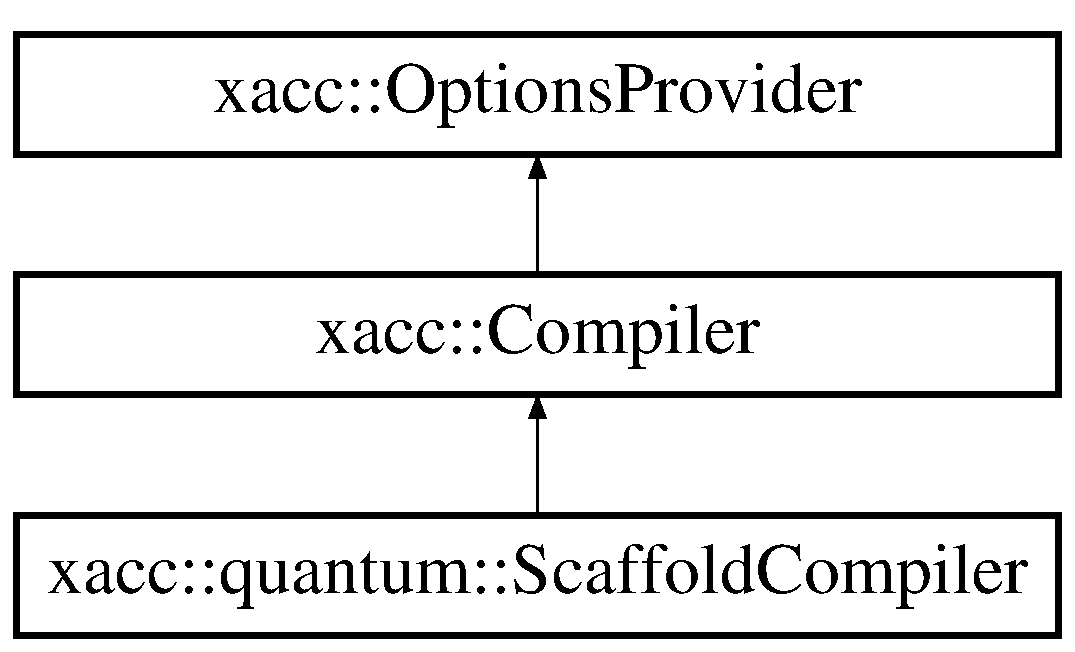
\includegraphics[height=3.000000cm]{a00078}
\end{center}
\end{figure}
\subsection*{Public Member Functions}
\begin{DoxyCompactItemize}
\item 
virtual std\+::shared\+\_\+ptr$<$ \hyperlink{a00051}{xacc\+::\+IR} $>$ \hyperlink{a00078_a7caede75bb2304ba405966651b115543}{compile} (const std\+::string \&src, std\+::shared\+\_\+ptr$<$ \hyperlink{a00011}{Accelerator} $>$ acc)
\item 
virtual std\+::shared\+\_\+ptr$<$ \hyperlink{a00051}{xacc\+::\+IR} $>$ \hyperlink{a00078_a3736ecc229fe6acdd4c991e85d7a1f08}{compile} (const std\+::string \&src)
\item 
virtual const std\+::string \hyperlink{a00078_ac7ca2941e987ba579c6f50cfbd7fb0dc}{translate} (const std\+::string \&buffer\+Variable, std\+::shared\+\_\+ptr$<$ \hyperlink{a00039}{Function} $>$ function)
\item 
virtual const std\+::string \hyperlink{a00078_a3f537054a3924a1d14f4ceb0f0181161}{get\+Name} ()
\item 
virtual \hyperlink{a00078_afb26398b07377ab9ddebc43a9376a6dd}{$\sim$\+Scaffold\+Compiler} ()
\end{DoxyCompactItemize}
\subsection*{Static Public Member Functions}
\begin{DoxyCompactItemize}
\item 
static void \hyperlink{a00078_aed16dda1e919e5af6de9953a656f62ce}{register\+Compiler} ()
\end{DoxyCompactItemize}
\subsection*{Protected Attributes}
\begin{DoxyCompactItemize}
\item 
std\+::shared\+\_\+ptr$<$ clang\+::\+Compiler\+Instance $>$ \hyperlink{a00078_af7a3a73eaab025a0ea72cc9335d8fbb4}{CI}
\item 
std\+::shared\+\_\+ptr$<$ \hyperlink{a00077}{Scaffold\+A\+S\+T\+Consumer} $>$ \hyperlink{a00078_ab1c4d36e58b97de50208e74a92d8ceb1}{consumer}
\end{DoxyCompactItemize}


\subsection{Detailed Description}
The Scaffold compiler is a subclass of the X\+A\+CC \hyperlink{a00023}{Compiler} that implements the \hyperlink{a00078_a7caede75bb2304ba405966651b115543}{compile()} and modify\+Source() methods to handle generation of quantum assembly language (or Q\+A\+SM) using an installed Scaffold compiler. 

\subsection{Constructor \& Destructor Documentation}
\index{xacc\+::quantum\+::\+Scaffold\+Compiler@{xacc\+::quantum\+::\+Scaffold\+Compiler}!````~Scaffold\+Compiler@{$\sim$\+Scaffold\+Compiler}}
\index{````~Scaffold\+Compiler@{$\sim$\+Scaffold\+Compiler}!xacc\+::quantum\+::\+Scaffold\+Compiler@{xacc\+::quantum\+::\+Scaffold\+Compiler}}
\subsubsection[{\texorpdfstring{$\sim$\+Scaffold\+Compiler()}{~ScaffoldCompiler()}}]{\setlength{\rightskip}{0pt plus 5cm}virtual xacc\+::quantum\+::\+Scaffold\+Compiler\+::$\sim$\+Scaffold\+Compiler (
\begin{DoxyParamCaption}
{}
\end{DoxyParamCaption}
)\hspace{0.3cm}{\ttfamily [inline]}, {\ttfamily [virtual]}}\hypertarget{a00078_afb26398b07377ab9ddebc43a9376a6dd}{}\label{a00078_afb26398b07377ab9ddebc43a9376a6dd}
The destructor 

\subsection{Member Function Documentation}
\index{xacc\+::quantum\+::\+Scaffold\+Compiler@{xacc\+::quantum\+::\+Scaffold\+Compiler}!compile@{compile}}
\index{compile@{compile}!xacc\+::quantum\+::\+Scaffold\+Compiler@{xacc\+::quantum\+::\+Scaffold\+Compiler}}
\subsubsection[{\texorpdfstring{compile(const std\+::string \&src, std\+::shared\+\_\+ptr$<$ Accelerator $>$ acc)}{compile(const std::string \&src, std::shared\_ptr< Accelerator > acc)}}]{\setlength{\rightskip}{0pt plus 5cm}std\+::shared\+\_\+ptr$<$ {\bf IR} $>$ xacc\+::quantum\+::\+Scaffold\+Compiler\+::compile (
\begin{DoxyParamCaption}
\item[{const std\+::string \&}]{src, }
\item[{std\+::shared\+\_\+ptr$<$ {\bf Accelerator} $>$}]{acc}
\end{DoxyParamCaption}
)\hspace{0.3cm}{\ttfamily [virtual]}}\hypertarget{a00078_a7caede75bb2304ba405966651b115543}{}\label{a00078_a7caede75bb2304ba405966651b115543}
Execute the Scaffold compiler to generate an X\+A\+CC intermediate representation instance. \begin{DoxyReturn}{Returns}
ir X\+A\+CC intermediate representation 
\end{DoxyReturn}


Implements \hyperlink{a00023_a546a40c95bb93af6a0c0ac48dbeaffc8}{xacc\+::\+Compiler}.

\index{xacc\+::quantum\+::\+Scaffold\+Compiler@{xacc\+::quantum\+::\+Scaffold\+Compiler}!compile@{compile}}
\index{compile@{compile}!xacc\+::quantum\+::\+Scaffold\+Compiler@{xacc\+::quantum\+::\+Scaffold\+Compiler}}
\subsubsection[{\texorpdfstring{compile(const std\+::string \&src)}{compile(const std::string \&src)}}]{\setlength{\rightskip}{0pt plus 5cm}std\+::shared\+\_\+ptr$<$ {\bf IR} $>$ xacc\+::quantum\+::\+Scaffold\+Compiler\+::compile (
\begin{DoxyParamCaption}
\item[{const std\+::string \&}]{src}
\end{DoxyParamCaption}
)\hspace{0.3cm}{\ttfamily [virtual]}}\hypertarget{a00078_a3736ecc229fe6acdd4c991e85d7a1f08}{}\label{a00078_a3736ecc229fe6acdd4c991e85d7a1f08}

\begin{DoxyParams}{Parameters}
{\em src} & \\
\hline
\end{DoxyParams}
\begin{DoxyReturn}{Returns}

\end{DoxyReturn}


Implements \hyperlink{a00023_a9092f5f779b570c91569b59621280c04}{xacc\+::\+Compiler}.

\index{xacc\+::quantum\+::\+Scaffold\+Compiler@{xacc\+::quantum\+::\+Scaffold\+Compiler}!get\+Name@{get\+Name}}
\index{get\+Name@{get\+Name}!xacc\+::quantum\+::\+Scaffold\+Compiler@{xacc\+::quantum\+::\+Scaffold\+Compiler}}
\subsubsection[{\texorpdfstring{get\+Name()}{getName()}}]{\setlength{\rightskip}{0pt plus 5cm}virtual const std\+::string xacc\+::quantum\+::\+Scaffold\+Compiler\+::get\+Name (
\begin{DoxyParamCaption}
{}
\end{DoxyParamCaption}
)\hspace{0.3cm}{\ttfamily [inline]}, {\ttfamily [virtual]}}\hypertarget{a00078_a3f537054a3924a1d14f4ceb0f0181161}{}\label{a00078_a3f537054a3924a1d14f4ceb0f0181161}
Return the name of this \hyperlink{a00023}{Compiler} \begin{DoxyReturn}{Returns}
name \hyperlink{a00023}{Compiler} name 
\end{DoxyReturn}


Implements \hyperlink{a00023_a87fca9100e6462122f5b687c3a0fb3fb}{xacc\+::\+Compiler}.

\index{xacc\+::quantum\+::\+Scaffold\+Compiler@{xacc\+::quantum\+::\+Scaffold\+Compiler}!register\+Compiler@{register\+Compiler}}
\index{register\+Compiler@{register\+Compiler}!xacc\+::quantum\+::\+Scaffold\+Compiler@{xacc\+::quantum\+::\+Scaffold\+Compiler}}
\subsubsection[{\texorpdfstring{register\+Compiler()}{registerCompiler()}}]{\setlength{\rightskip}{0pt plus 5cm}static void xacc\+::quantum\+::\+Scaffold\+Compiler\+::register\+Compiler (
\begin{DoxyParamCaption}
{}
\end{DoxyParamCaption}
)\hspace{0.3cm}{\ttfamily [inline]}, {\ttfamily [static]}}\hypertarget{a00078_aed16dda1e919e5af6de9953a656f62ce}{}\label{a00078_aed16dda1e919e5af6de9953a656f62ce}
Register this \hyperlink{a00023}{Compiler} with the framework. \index{xacc\+::quantum\+::\+Scaffold\+Compiler@{xacc\+::quantum\+::\+Scaffold\+Compiler}!translate@{translate}}
\index{translate@{translate}!xacc\+::quantum\+::\+Scaffold\+Compiler@{xacc\+::quantum\+::\+Scaffold\+Compiler}}
\subsubsection[{\texorpdfstring{translate(const std\+::string \&buffer\+Variable, std\+::shared\+\_\+ptr$<$ Function $>$ function)}{translate(const std::string \&bufferVariable, std::shared\_ptr< Function > function)}}]{\setlength{\rightskip}{0pt plus 5cm}const std\+::string xacc\+::quantum\+::\+Scaffold\+Compiler\+::translate (
\begin{DoxyParamCaption}
\item[{const std\+::string \&}]{buffer\+Variable, }
\item[{std\+::shared\+\_\+ptr$<$ {\bf Function} $>$}]{function}
\end{DoxyParamCaption}
)\hspace{0.3cm}{\ttfamily [virtual]}}\hypertarget{a00078_ac7ca2941e987ba579c6f50cfbd7fb0dc}{}\label{a00078_ac7ca2941e987ba579c6f50cfbd7fb0dc}
This produces a Scaffold source code representation of the given \hyperlink{a00051}{IR} \hyperlink{a00039}{Function}


\begin{DoxyParams}{Parameters}
{\em function} & The X\+A\+CC \hyperlink{a00051}{IR} \hyperlink{a00039}{Function} to translate \\
\hline
\end{DoxyParams}
\begin{DoxyReturn}{Returns}
src The source code as a string 
\end{DoxyReturn}


Implements \hyperlink{a00023_aeedbe58a33fed29e4d7694ae743e25e7}{xacc\+::\+Compiler}.



\subsection{Member Data Documentation}
\index{xacc\+::quantum\+::\+Scaffold\+Compiler@{xacc\+::quantum\+::\+Scaffold\+Compiler}!CI@{CI}}
\index{CI@{CI}!xacc\+::quantum\+::\+Scaffold\+Compiler@{xacc\+::quantum\+::\+Scaffold\+Compiler}}
\subsubsection[{\texorpdfstring{CI}{CI}}]{\setlength{\rightskip}{0pt plus 5cm}std\+::shared\+\_\+ptr$<$clang\+::\+Compiler\+Instance$>$ xacc\+::quantum\+::\+Scaffold\+Compiler\+::\+CI\hspace{0.3cm}{\ttfamily [protected]}}\hypertarget{a00078_af7a3a73eaab025a0ea72cc9335d8fbb4}{}\label{a00078_af7a3a73eaab025a0ea72cc9335d8fbb4}
Reference to the Scaffold Clang \hyperlink{a00023}{Compiler} \index{xacc\+::quantum\+::\+Scaffold\+Compiler@{xacc\+::quantum\+::\+Scaffold\+Compiler}!consumer@{consumer}}
\index{consumer@{consumer}!xacc\+::quantum\+::\+Scaffold\+Compiler@{xacc\+::quantum\+::\+Scaffold\+Compiler}}
\subsubsection[{\texorpdfstring{consumer}{consumer}}]{\setlength{\rightskip}{0pt plus 5cm}std\+::shared\+\_\+ptr$<${\bf Scaffold\+A\+S\+T\+Consumer}$>$ xacc\+::quantum\+::\+Scaffold\+Compiler\+::consumer\hspace{0.3cm}{\ttfamily [protected]}}\hypertarget{a00078_ab1c4d36e58b97de50208e74a92d8ceb1}{}\label{a00078_ab1c4d36e58b97de50208e74a92d8ceb1}
Reference to our A\+ST Consumer, this gives us the compiled \hyperlink{a00051}{IR} \hyperlink{a00039}{Function} and the Qubit Variable Name 

The documentation for this class was generated from the following files\+:\begin{DoxyCompactItemize}
\item 
Scaffold\+Compiler.\+hpp\item 
Scaffold\+Compiler.\+cpp\end{DoxyCompactItemize}

\hypertarget{a00079}{}\section{xacc\+:\+:quantum\+:\+:Scaffold\+I\+R\+To\+Src\+Visitor Class Reference}
\label{a00079}\index{xacc\+::quantum\+::\+Scaffold\+I\+R\+To\+Src\+Visitor@{xacc\+::quantum\+::\+Scaffold\+I\+R\+To\+Src\+Visitor}}


{\ttfamily \#include $<$Scaffold\+I\+R\+To\+Src\+Visitor.\+hpp$>$}

Inheritance diagram for xacc\+:\+:quantum\+:\+:Scaffold\+I\+R\+To\+Src\+Visitor\+:\begin{figure}[H]
\begin{center}
\leavevmode
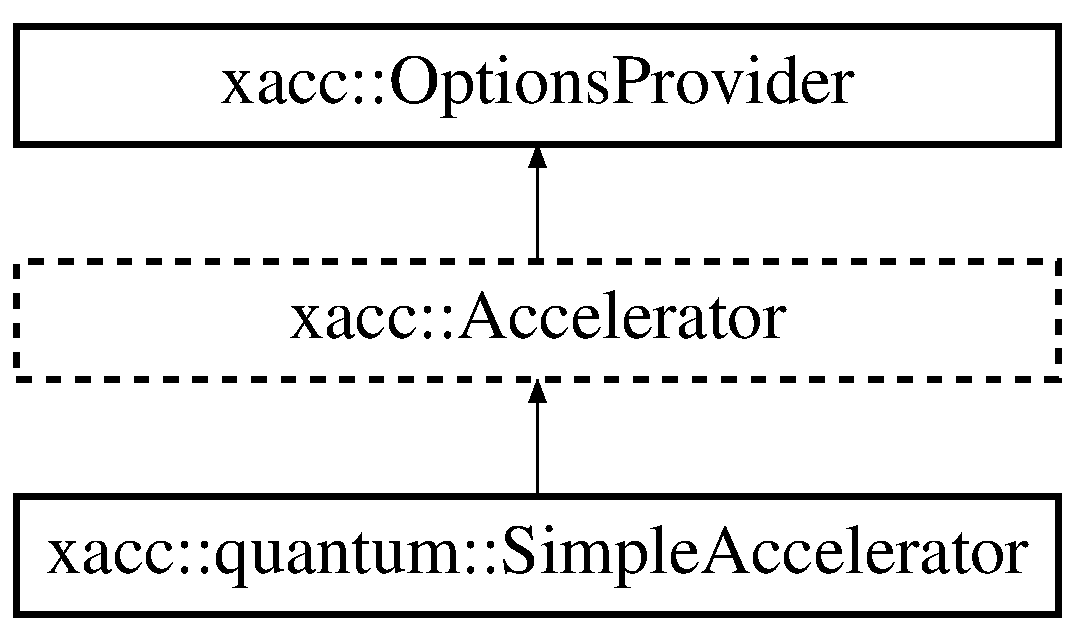
\includegraphics[height=12.000000cm]{a00079}
\end{center}
\end{figure}
\subsection*{Public Member Functions}
\begin{DoxyCompactItemize}
\item 
{\bfseries Scaffold\+I\+R\+To\+Src\+Visitor} (std\+::string var)\hypertarget{a00079_a38e9a5775397847973f78856e4b0031e}{}\label{a00079_a38e9a5775397847973f78856e4b0031e}

\item 
void \hyperlink{a00079_af66cbe08e183c8b53817cda5251d0498}{visit} (\hyperlink{a00045}{Hadamard} \&h)
\item 
void \hyperlink{a00079_a81b16c7a7da2c84174796ef4cc39b312}{visit} (\hyperlink{a00022}{C\+N\+OT} \&cn)
\item 
void \hyperlink{a00079_a1a414fa079f0e3ba8cd0f97c7928e88f}{visit} (\hyperlink{a00085}{X} \&x)
\item 
void {\bfseries visit} (\hyperlink{a00088}{Y} \&y)\hypertarget{a00079_a9130f70ceaa42bdc3c29c8b0bbdcc3b5}{}\label{a00079_a9130f70ceaa42bdc3c29c8b0bbdcc3b5}

\item 
void \hyperlink{a00079_a444936ec9134a0ea400cd2f1b145ba4d}{visit} (\hyperlink{a00089}{Z} \&z)
\item 
void \hyperlink{a00079_a99e7176144810f5d6e38d98d2725afff}{visit} (\hyperlink{a00056}{Measure} \&m)
\item 
void \hyperlink{a00079_a1646dbfaf919432c2c3d8eb86e9f81e4}{visit} (\hyperlink{a00025}{Conditional\+Function} \&c)
\item 
void {\bfseries visit} (\hyperlink{a00074}{Rx} \&rx)\hypertarget{a00079_afc1ace9f5cb4783117a68b173c069d15}{}\label{a00079_afc1ace9f5cb4783117a68b173c069d15}

\item 
void {\bfseries visit} (\hyperlink{a00075}{Ry} \&ry)\hypertarget{a00079_a08539d478a1b496244288477ccee8011}{}\label{a00079_a08539d478a1b496244288477ccee8011}

\item 
void {\bfseries visit} (\hyperlink{a00076}{Rz} \&rz)\hypertarget{a00079_a855cbf9e83b050ae65e95c4a36f02de9}{}\label{a00079_a855cbf9e83b050ae65e95c4a36f02de9}

\item 
void {\bfseries visit} (\hyperlink{a00027}{C\+Phase} \&cp)\hypertarget{a00079_a4d8e2c6d867d812aeca192ebc65a45ce}{}\label{a00079_a4d8e2c6d867d812aeca192ebc65a45ce}

\item 
void {\bfseries visit} (\hyperlink{a00083}{Swap} \&s)\hypertarget{a00079_a502e0145245e4aa00af4f76e1b201e7a}{}\label{a00079_a502e0145245e4aa00af4f76e1b201e7a}

\item 
void {\bfseries visit} (\hyperlink{a00041}{Gate\+Function} \&f)\hypertarget{a00079_adf65b4117c2dfd3242c5c214eef608c5}{}\label{a00079_adf65b4117c2dfd3242c5c214eef608c5}

\item 
std\+::string \hyperlink{a00079_ad721b67dae6360ce210d6c73feec7920}{get\+Scaffold\+String} ()
\item 
virtual \hyperlink{a00079_a366cddf574488b3bf0df1fe991806753}{$\sim$\+Scaffold\+I\+R\+To\+Src\+Visitor} ()
\end{DoxyCompactItemize}
\subsection*{Protected Member Functions}
\begin{DoxyCompactItemize}
\item 
void {\bfseries base\+Instruction} (std\+::string gate\+Name, std\+::vector$<$ int $>$ qubits)\hypertarget{a00079_afa951f637b70233cfded3c05177e2b56}{}\label{a00079_afa951f637b70233cfded3c05177e2b56}

\item 
void {\bfseries base\+Parameterized\+Instruction} (std\+::string gate\+Name, std\+::vector$<$ int $>$ qubits, std\+::vector$<$ Instruction\+Parameter $>$ params)\hypertarget{a00079_a23d8435f4696290c32afdae1abfbff30}{}\label{a00079_a23d8435f4696290c32afdae1abfbff30}

\end{DoxyCompactItemize}
\subsection*{Protected Attributes}
\begin{DoxyCompactItemize}
\item 
std\+::string \hyperlink{a00079_a4b4c3b769a275d544beb26b1894e476a}{scaffold\+Str}
\item 
std\+::string {\bfseries qubit\+Var\+Name}\hypertarget{a00079_ab538cf6fe8606e9832310a8195b67dce}{}\label{a00079_ab538cf6fe8606e9832310a8195b67dce}

\item 
int {\bfseries n\+Measurements} = 0\hypertarget{a00079_ae7d177fa9830942f63ef86fd2f69f715}{}\label{a00079_ae7d177fa9830942f63ef86fd2f69f715}

\item 
std\+::map$<$ int, int $>$ {\bfseries qubit\+To\+Classical\+Bit\+Index}\hypertarget{a00079_a76945624d8d67487d410a11a91e97681}{}\label{a00079_a76945624d8d67487d410a11a91e97681}

\end{DoxyCompactItemize}


\subsection{Detailed Description}
The \hyperlink{a00064}{Quil\+Visitor} is an \hyperlink{a00049}{Instruction\+Visitor} that visits quantum gate instructions and creates an equivalent Quil string that can be executed by the Rigetti superconducting quantum computer. 

\subsection{Constructor \& Destructor Documentation}
\index{xacc\+::quantum\+::\+Scaffold\+I\+R\+To\+Src\+Visitor@{xacc\+::quantum\+::\+Scaffold\+I\+R\+To\+Src\+Visitor}!````~Scaffold\+I\+R\+To\+Src\+Visitor@{$\sim$\+Scaffold\+I\+R\+To\+Src\+Visitor}}
\index{````~Scaffold\+I\+R\+To\+Src\+Visitor@{$\sim$\+Scaffold\+I\+R\+To\+Src\+Visitor}!xacc\+::quantum\+::\+Scaffold\+I\+R\+To\+Src\+Visitor@{xacc\+::quantum\+::\+Scaffold\+I\+R\+To\+Src\+Visitor}}
\subsubsection[{\texorpdfstring{$\sim$\+Scaffold\+I\+R\+To\+Src\+Visitor()}{~ScaffoldIRToSrcVisitor()}}]{\setlength{\rightskip}{0pt plus 5cm}virtual xacc\+::quantum\+::\+Scaffold\+I\+R\+To\+Src\+Visitor\+::$\sim$\+Scaffold\+I\+R\+To\+Src\+Visitor (
\begin{DoxyParamCaption}
{}
\end{DoxyParamCaption}
)\hspace{0.3cm}{\ttfamily [inline]}, {\ttfamily [virtual]}}\hypertarget{a00079_a366cddf574488b3bf0df1fe991806753}{}\label{a00079_a366cddf574488b3bf0df1fe991806753}
The destructor 

\subsection{Member Function Documentation}
\index{xacc\+::quantum\+::\+Scaffold\+I\+R\+To\+Src\+Visitor@{xacc\+::quantum\+::\+Scaffold\+I\+R\+To\+Src\+Visitor}!get\+Scaffold\+String@{get\+Scaffold\+String}}
\index{get\+Scaffold\+String@{get\+Scaffold\+String}!xacc\+::quantum\+::\+Scaffold\+I\+R\+To\+Src\+Visitor@{xacc\+::quantum\+::\+Scaffold\+I\+R\+To\+Src\+Visitor}}
\subsubsection[{\texorpdfstring{get\+Scaffold\+String()}{getScaffoldString()}}]{\setlength{\rightskip}{0pt plus 5cm}std\+::string xacc\+::quantum\+::\+Scaffold\+I\+R\+To\+Src\+Visitor\+::get\+Scaffold\+String (
\begin{DoxyParamCaption}
{}
\end{DoxyParamCaption}
)\hspace{0.3cm}{\ttfamily [inline]}}\hypertarget{a00079_ad721b67dae6360ce210d6c73feec7920}{}\label{a00079_ad721b67dae6360ce210d6c73feec7920}
Return the quil string \index{xacc\+::quantum\+::\+Scaffold\+I\+R\+To\+Src\+Visitor@{xacc\+::quantum\+::\+Scaffold\+I\+R\+To\+Src\+Visitor}!visit@{visit}}
\index{visit@{visit}!xacc\+::quantum\+::\+Scaffold\+I\+R\+To\+Src\+Visitor@{xacc\+::quantum\+::\+Scaffold\+I\+R\+To\+Src\+Visitor}}
\subsubsection[{\texorpdfstring{visit(\+Hadamard \&h)}{visit(Hadamard \&h)}}]{\setlength{\rightskip}{0pt plus 5cm}void xacc\+::quantum\+::\+Scaffold\+I\+R\+To\+Src\+Visitor\+::visit (
\begin{DoxyParamCaption}
\item[{{\bf Hadamard} \&}]{h}
\end{DoxyParamCaption}
)\hspace{0.3cm}{\ttfamily [inline]}}\hypertarget{a00079_af66cbe08e183c8b53817cda5251d0498}{}\label{a00079_af66cbe08e183c8b53817cda5251d0498}
Visit hadamard gates \index{xacc\+::quantum\+::\+Scaffold\+I\+R\+To\+Src\+Visitor@{xacc\+::quantum\+::\+Scaffold\+I\+R\+To\+Src\+Visitor}!visit@{visit}}
\index{visit@{visit}!xacc\+::quantum\+::\+Scaffold\+I\+R\+To\+Src\+Visitor@{xacc\+::quantum\+::\+Scaffold\+I\+R\+To\+Src\+Visitor}}
\subsubsection[{\texorpdfstring{visit(\+C\+N\+O\+T \&cn)}{visit(CNOT \&cn)}}]{\setlength{\rightskip}{0pt plus 5cm}void xacc\+::quantum\+::\+Scaffold\+I\+R\+To\+Src\+Visitor\+::visit (
\begin{DoxyParamCaption}
\item[{{\bf C\+N\+OT} \&}]{cn}
\end{DoxyParamCaption}
)\hspace{0.3cm}{\ttfamily [inline]}}\hypertarget{a00079_a81b16c7a7da2c84174796ef4cc39b312}{}\label{a00079_a81b16c7a7da2c84174796ef4cc39b312}
Visit \hyperlink{a00022}{C\+N\+OT} gates \index{xacc\+::quantum\+::\+Scaffold\+I\+R\+To\+Src\+Visitor@{xacc\+::quantum\+::\+Scaffold\+I\+R\+To\+Src\+Visitor}!visit@{visit}}
\index{visit@{visit}!xacc\+::quantum\+::\+Scaffold\+I\+R\+To\+Src\+Visitor@{xacc\+::quantum\+::\+Scaffold\+I\+R\+To\+Src\+Visitor}}
\subsubsection[{\texorpdfstring{visit(\+X \&x)}{visit(X \&x)}}]{\setlength{\rightskip}{0pt plus 5cm}void xacc\+::quantum\+::\+Scaffold\+I\+R\+To\+Src\+Visitor\+::visit (
\begin{DoxyParamCaption}
\item[{{\bf X} \&}]{x}
\end{DoxyParamCaption}
)\hspace{0.3cm}{\ttfamily [inline]}}\hypertarget{a00079_a1a414fa079f0e3ba8cd0f97c7928e88f}{}\label{a00079_a1a414fa079f0e3ba8cd0f97c7928e88f}
Visit \hyperlink{a00085}{X} gates \index{xacc\+::quantum\+::\+Scaffold\+I\+R\+To\+Src\+Visitor@{xacc\+::quantum\+::\+Scaffold\+I\+R\+To\+Src\+Visitor}!visit@{visit}}
\index{visit@{visit}!xacc\+::quantum\+::\+Scaffold\+I\+R\+To\+Src\+Visitor@{xacc\+::quantum\+::\+Scaffold\+I\+R\+To\+Src\+Visitor}}
\subsubsection[{\texorpdfstring{visit(\+Z \&z)}{visit(Z \&z)}}]{\setlength{\rightskip}{0pt plus 5cm}void xacc\+::quantum\+::\+Scaffold\+I\+R\+To\+Src\+Visitor\+::visit (
\begin{DoxyParamCaption}
\item[{{\bf Z} \&}]{z}
\end{DoxyParamCaption}
)\hspace{0.3cm}{\ttfamily [inline]}}\hypertarget{a00079_a444936ec9134a0ea400cd2f1b145ba4d}{}\label{a00079_a444936ec9134a0ea400cd2f1b145ba4d}
Visit \hyperlink{a00089}{Z} gates \index{xacc\+::quantum\+::\+Scaffold\+I\+R\+To\+Src\+Visitor@{xacc\+::quantum\+::\+Scaffold\+I\+R\+To\+Src\+Visitor}!visit@{visit}}
\index{visit@{visit}!xacc\+::quantum\+::\+Scaffold\+I\+R\+To\+Src\+Visitor@{xacc\+::quantum\+::\+Scaffold\+I\+R\+To\+Src\+Visitor}}
\subsubsection[{\texorpdfstring{visit(\+Measure \&m)}{visit(Measure \&m)}}]{\setlength{\rightskip}{0pt plus 5cm}void xacc\+::quantum\+::\+Scaffold\+I\+R\+To\+Src\+Visitor\+::visit (
\begin{DoxyParamCaption}
\item[{{\bf Measure} \&}]{m}
\end{DoxyParamCaption}
)\hspace{0.3cm}{\ttfamily [inline]}}\hypertarget{a00079_a99e7176144810f5d6e38d98d2725afff}{}\label{a00079_a99e7176144810f5d6e38d98d2725afff}
Visit Measurement gates \index{xacc\+::quantum\+::\+Scaffold\+I\+R\+To\+Src\+Visitor@{xacc\+::quantum\+::\+Scaffold\+I\+R\+To\+Src\+Visitor}!visit@{visit}}
\index{visit@{visit}!xacc\+::quantum\+::\+Scaffold\+I\+R\+To\+Src\+Visitor@{xacc\+::quantum\+::\+Scaffold\+I\+R\+To\+Src\+Visitor}}
\subsubsection[{\texorpdfstring{visit(\+Conditional\+Function \&c)}{visit(ConditionalFunction \&c)}}]{\setlength{\rightskip}{0pt plus 5cm}void xacc\+::quantum\+::\+Scaffold\+I\+R\+To\+Src\+Visitor\+::visit (
\begin{DoxyParamCaption}
\item[{{\bf Conditional\+Function} \&}]{c}
\end{DoxyParamCaption}
)\hspace{0.3cm}{\ttfamily [inline]}}\hypertarget{a00079_a1646dbfaf919432c2c3d8eb86e9f81e4}{}\label{a00079_a1646dbfaf919432c2c3d8eb86e9f81e4}
Visit Conditional functions 

\subsection{Member Data Documentation}
\index{xacc\+::quantum\+::\+Scaffold\+I\+R\+To\+Src\+Visitor@{xacc\+::quantum\+::\+Scaffold\+I\+R\+To\+Src\+Visitor}!scaffold\+Str@{scaffold\+Str}}
\index{scaffold\+Str@{scaffold\+Str}!xacc\+::quantum\+::\+Scaffold\+I\+R\+To\+Src\+Visitor@{xacc\+::quantum\+::\+Scaffold\+I\+R\+To\+Src\+Visitor}}
\subsubsection[{\texorpdfstring{scaffold\+Str}{scaffoldStr}}]{\setlength{\rightskip}{0pt plus 5cm}std\+::string xacc\+::quantum\+::\+Scaffold\+I\+R\+To\+Src\+Visitor\+::scaffold\+Str\hspace{0.3cm}{\ttfamily [protected]}}\hypertarget{a00079_a4b4c3b769a275d544beb26b1894e476a}{}\label{a00079_a4b4c3b769a275d544beb26b1894e476a}
Reference to the Quil string this visitor is trying to construct 

The documentation for this class was generated from the following file\+:\begin{DoxyCompactItemize}
\item 
Scaffold\+I\+R\+To\+Src\+Visitor.\+hpp\end{DoxyCompactItemize}

\hypertarget{a00080}{}\section{xacc\+:\+:quantum\+:\+:D\+Wave\+Compiler Class Reference}
\label{a00080}\index{xacc\+::quantum\+::\+D\+Wave\+Compiler@{xacc\+::quantum\+::\+D\+Wave\+Compiler}}
Inheritance diagram for xacc\+:\+:quantum\+:\+:D\+Wave\+Compiler\+:\begin{figure}[H]
\begin{center}
\leavevmode
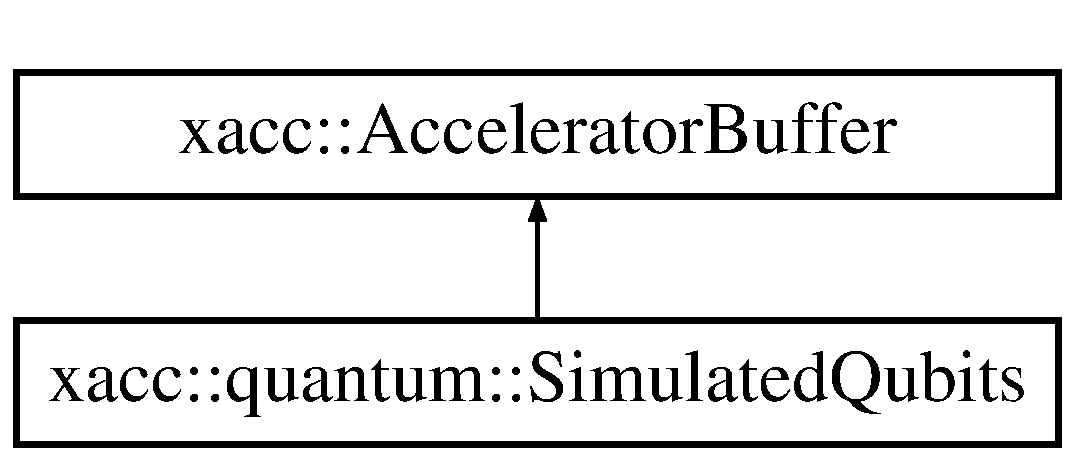
\includegraphics[height=3.000000cm]{a00080}
\end{center}
\end{figure}
\subsection*{Public Member Functions}
\begin{DoxyCompactItemize}
\item 
virtual std\+::shared\+\_\+ptr$<$ \hyperlink{a00167}{xacc\+::\+IR} $>$ \hyperlink{a00080_a0f7f6b10b4a881cb27b36eaa6d39e7b1}{compile} (const std\+::string \&src, std\+::shared\+\_\+ptr$<$ \hyperlink{a00030}{Accelerator} $>$ acc)
\item 
virtual std\+::shared\+\_\+ptr$<$ \hyperlink{a00167}{xacc\+::\+IR} $>$ \hyperlink{a00080_a893e1d1c81a8aaf6e2435c9bceab575e}{compile} (const std\+::string \&src)
\item 
virtual const std\+::string \hyperlink{a00080_a8a180031ae563e1a9aac611e8066c181}{get\+Name} ()
\item 
virtual \hyperlink{a00080_acc0ab28f787b8f4cbeb63c594a247e50}{$\sim$\+D\+Wave\+Compiler} ()
\end{DoxyCompactItemize}
\subsection*{Static Public Member Functions}
\begin{DoxyCompactItemize}
\item 
static void \hyperlink{a00080_a5b221649f22a9bb4d4a304a6522d071f}{register\+Compiler} ()
\end{DoxyCompactItemize}
\subsection*{Additional Inherited Members}


\subsection{Constructor \& Destructor Documentation}
\index{xacc\+::quantum\+::\+D\+Wave\+Compiler@{xacc\+::quantum\+::\+D\+Wave\+Compiler}!````~D\+Wave\+Compiler@{$\sim$\+D\+Wave\+Compiler}}
\index{````~D\+Wave\+Compiler@{$\sim$\+D\+Wave\+Compiler}!xacc\+::quantum\+::\+D\+Wave\+Compiler@{xacc\+::quantum\+::\+D\+Wave\+Compiler}}
\subsubsection[{\texorpdfstring{$\sim$\+D\+Wave\+Compiler()}{~DWaveCompiler()}}]{\setlength{\rightskip}{0pt plus 5cm}virtual xacc\+::quantum\+::\+D\+Wave\+Compiler\+::$\sim$\+D\+Wave\+Compiler (
\begin{DoxyParamCaption}
{}
\end{DoxyParamCaption}
)\hspace{0.3cm}{\ttfamily [inline]}, {\ttfamily [virtual]}}\hypertarget{a00080_acc0ab28f787b8f4cbeb63c594a247e50}{}\label{a00080_acc0ab28f787b8f4cbeb63c594a247e50}
The destructor 

\subsection{Member Function Documentation}
\index{xacc\+::quantum\+::\+D\+Wave\+Compiler@{xacc\+::quantum\+::\+D\+Wave\+Compiler}!compile@{compile}}
\index{compile@{compile}!xacc\+::quantum\+::\+D\+Wave\+Compiler@{xacc\+::quantum\+::\+D\+Wave\+Compiler}}
\subsubsection[{\texorpdfstring{compile(const std\+::string \&src, std\+::shared\+\_\+ptr$<$ Accelerator $>$ acc)}{compile(const std::string \&src, std::shared\_ptr< Accelerator > acc)}}]{\setlength{\rightskip}{0pt plus 5cm}std\+::shared\+\_\+ptr$<$ {\bf IR} $>$ xacc\+::quantum\+::\+D\+Wave\+Compiler\+::compile (
\begin{DoxyParamCaption}
\item[{const std\+::string \&}]{src, }
\item[{std\+::shared\+\_\+ptr$<$ {\bf Accelerator} $>$}]{acc}
\end{DoxyParamCaption}
)\hspace{0.3cm}{\ttfamily [virtual]}}\hypertarget{a00080_a0f7f6b10b4a881cb27b36eaa6d39e7b1}{}\label{a00080_a0f7f6b10b4a881cb27b36eaa6d39e7b1}
This method is to be implemented by derived Compilers and is in charge of executing the compilation mechanism on the provided source string. Implementations also are given access to the \hyperlink{a00030}{Accelerator} that this source code is intended for.


\begin{DoxyParams}{Parameters}
{\em src} & The kernel source string. \\
\hline
{\em acc} & The \hyperlink{a00030}{Accelerator} this code will be executed on \\
\hline
\end{DoxyParams}
\begin{DoxyReturn}{Returns}
ir Intermediate representation for provided source kernel code. 
\end{DoxyReturn}


Implements \hyperlink{a00059_a546a40c95bb93af6a0c0ac48dbeaffc8}{xacc\+::\+Compiler}.

\index{xacc\+::quantum\+::\+D\+Wave\+Compiler@{xacc\+::quantum\+::\+D\+Wave\+Compiler}!compile@{compile}}
\index{compile@{compile}!xacc\+::quantum\+::\+D\+Wave\+Compiler@{xacc\+::quantum\+::\+D\+Wave\+Compiler}}
\subsubsection[{\texorpdfstring{compile(const std\+::string \&src)}{compile(const std::string \&src)}}]{\setlength{\rightskip}{0pt plus 5cm}std\+::shared\+\_\+ptr$<$ {\bf IR} $>$ xacc\+::quantum\+::\+D\+Wave\+Compiler\+::compile (
\begin{DoxyParamCaption}
\item[{const std\+::string \&}]{src}
\end{DoxyParamCaption}
)\hspace{0.3cm}{\ttfamily [virtual]}}\hypertarget{a00080_a893e1d1c81a8aaf6e2435c9bceab575e}{}\label{a00080_a893e1d1c81a8aaf6e2435c9bceab575e}
\begin{DoxyReturn}{Returns}

\end{DoxyReturn}


Implements \hyperlink{a00059_a9092f5f779b570c91569b59621280c04}{xacc\+::\+Compiler}.

\index{xacc\+::quantum\+::\+D\+Wave\+Compiler@{xacc\+::quantum\+::\+D\+Wave\+Compiler}!get\+Name@{get\+Name}}
\index{get\+Name@{get\+Name}!xacc\+::quantum\+::\+D\+Wave\+Compiler@{xacc\+::quantum\+::\+D\+Wave\+Compiler}}
\subsubsection[{\texorpdfstring{get\+Name()}{getName()}}]{\setlength{\rightskip}{0pt plus 5cm}virtual const std\+::string xacc\+::quantum\+::\+D\+Wave\+Compiler\+::get\+Name (
\begin{DoxyParamCaption}
{}
\end{DoxyParamCaption}
)\hspace{0.3cm}{\ttfamily [inline]}, {\ttfamily [virtual]}}\hypertarget{a00080_a8a180031ae563e1a9aac611e8066c181}{}\label{a00080_a8a180031ae563e1a9aac611e8066c181}
Return the name of this \hyperlink{a00059}{Compiler} \begin{DoxyReturn}{Returns}
name \hyperlink{a00059}{Compiler} name 
\end{DoxyReturn}


Implements \hyperlink{a00059_a87fca9100e6462122f5b687c3a0fb3fb}{xacc\+::\+Compiler}.

\index{xacc\+::quantum\+::\+D\+Wave\+Compiler@{xacc\+::quantum\+::\+D\+Wave\+Compiler}!register\+Compiler@{register\+Compiler}}
\index{register\+Compiler@{register\+Compiler}!xacc\+::quantum\+::\+D\+Wave\+Compiler@{xacc\+::quantum\+::\+D\+Wave\+Compiler}}
\subsubsection[{\texorpdfstring{register\+Compiler()}{registerCompiler()}}]{\setlength{\rightskip}{0pt plus 5cm}static void xacc\+::quantum\+::\+D\+Wave\+Compiler\+::register\+Compiler (
\begin{DoxyParamCaption}
{}
\end{DoxyParamCaption}
)\hspace{0.3cm}{\ttfamily [inline]}, {\ttfamily [static]}}\hypertarget{a00080_a5b221649f22a9bb4d4a304a6522d071f}{}\label{a00080_a5b221649f22a9bb4d4a304a6522d071f}
Register this \hyperlink{a00059}{Compiler} with the framework. 

The documentation for this class was generated from the following files\+:\begin{DoxyCompactItemize}
\item 
D\+Wave\+Compiler.\+hpp\item 
D\+Wave\+Compiler.\+cpp\end{DoxyCompactItemize}

\hypertarget{a00081}{}\section{xacc\+:\+:quantum\+:\+:Simulated\+Qubits Class Reference}
\label{a00081}\index{xacc\+::quantum\+::\+Simulated\+Qubits@{xacc\+::quantum\+::\+Simulated\+Qubits}}


{\ttfamily \#include $<$Simulated\+Qubits.\+hpp$>$}

Inheritance diagram for xacc\+:\+:quantum\+:\+:Simulated\+Qubits\+:\begin{figure}[H]
\begin{center}
\leavevmode
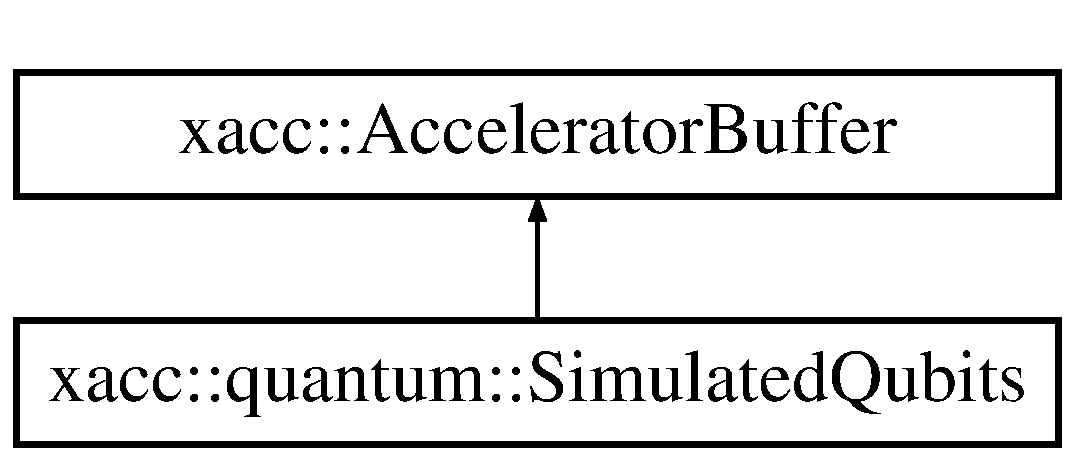
\includegraphics[height=2.000000cm]{a00081}
\end{center}
\end{figure}
\subsection*{Public Member Functions}
\begin{DoxyCompactItemize}
\item 
\hyperlink{a00081_abb0419229628210a1c187b76be6edc30}{Simulated\+Qubits} (const std\+::string \&str, const int N)
\item 
{\footnotesize template$<$typename... Indices$>$ }\\\hyperlink{a00081_ae11d09c17316adb09b93cc866969dba8}{Simulated\+Qubits} (const std\+::string \&str, int first\+Index, Indices...\+indices)
\item 
void \hyperlink{a00081_a3f4518d0135101141bf92d7e31f4fddc}{apply\+Unitary} (fire\+::\+Tensor$<$ 2, fire\+::\+Eigen\+Provider, std\+::complex$<$ double $>$$>$ \&U)
\item 
void \hyperlink{a00081_a09ee499769bb1eedaf08d6b5c29f9791}{normalize} ()
\item 
Qubit\+State \& \hyperlink{a00081_a405577717ca200ed9e524c04209e0216}{get\+State} ()
\item 
void \hyperlink{a00081_a8cd74c239c1fcecb3d03d6989732d5fe}{set\+State} (Qubit\+State \&st)
\item 
virtual void \hyperlink{a00081_a9252d30be0563f36bf1ff839c7104cd7}{print} (std\+::ostream \&stream)
\item 
virtual void \hyperlink{a00081_a32922bd2ccc64bba601c07a3c136cc3d}{print} ()
\item 
virtual \hyperlink{a00081_aebf6f30a6d8c84971091d87908680e7e}{$\sim$\+Simulated\+Qubits} ()
\end{DoxyCompactItemize}
\subsection*{Protected Attributes}
\begin{DoxyCompactItemize}
\item 
Qubit\+State \hyperlink{a00081_a630bea50ee06fd59f74450f01f95e489}{buffer\+State}
\end{DoxyCompactItemize}


\subsection{Detailed Description}
\hyperlink{a00081}{Simulated\+Qubits} is an \hyperlink{a00013}{Accelerator\+Buffer} that models simulated qubits. As such, it keeps track of the state of the qubit buffer using a Rank 1 Fire Tensor.

It provides an interface for applying unitary operations on the qubit buffer state. 

\subsection{Constructor \& Destructor Documentation}
\index{xacc\+::quantum\+::\+Simulated\+Qubits@{xacc\+::quantum\+::\+Simulated\+Qubits}!Simulated\+Qubits@{Simulated\+Qubits}}
\index{Simulated\+Qubits@{Simulated\+Qubits}!xacc\+::quantum\+::\+Simulated\+Qubits@{xacc\+::quantum\+::\+Simulated\+Qubits}}
\subsubsection[{\texorpdfstring{Simulated\+Qubits(const std\+::string \&str, const int N)}{SimulatedQubits(const std::string \&str, const int N)}}]{\setlength{\rightskip}{0pt plus 5cm}xacc\+::quantum\+::\+Simulated\+Qubits\+::\+Simulated\+Qubits (
\begin{DoxyParamCaption}
\item[{const std\+::string \&}]{str, }
\item[{const int}]{N}
\end{DoxyParamCaption}
)\hspace{0.3cm}{\ttfamily [inline]}}\hypertarget{a00081_abb0419229628210a1c187b76be6edc30}{}\label{a00081_abb0419229628210a1c187b76be6edc30}
The Constructor, creates a state with given size N. 
\begin{DoxyParams}{Parameters}
{\em str} & Variable name of this buffer \\
\hline
{\em N} & The number of qubits to model \\
\hline
\end{DoxyParams}
\index{xacc\+::quantum\+::\+Simulated\+Qubits@{xacc\+::quantum\+::\+Simulated\+Qubits}!Simulated\+Qubits@{Simulated\+Qubits}}
\index{Simulated\+Qubits@{Simulated\+Qubits}!xacc\+::quantum\+::\+Simulated\+Qubits@{xacc\+::quantum\+::\+Simulated\+Qubits}}
\subsubsection[{\texorpdfstring{Simulated\+Qubits(const std\+::string \&str, int first\+Index, Indices...\+indices)}{SimulatedQubits(const std::string \&str, int firstIndex, Indices...indices)}}]{\setlength{\rightskip}{0pt plus 5cm}template$<$typename... Indices$>$ xacc\+::quantum\+::\+Simulated\+Qubits\+::\+Simulated\+Qubits (
\begin{DoxyParamCaption}
\item[{const std\+::string \&}]{str, }
\item[{int}]{first\+Index, }
\item[{Indices...}]{indices}
\end{DoxyParamCaption}
)\hspace{0.3cm}{\ttfamily [inline]}}\hypertarget{a00081_ae11d09c17316adb09b93cc866969dba8}{}\label{a00081_ae11d09c17316adb09b93cc866969dba8}
The constructor \index{xacc\+::quantum\+::\+Simulated\+Qubits@{xacc\+::quantum\+::\+Simulated\+Qubits}!````~Simulated\+Qubits@{$\sim$\+Simulated\+Qubits}}
\index{````~Simulated\+Qubits@{$\sim$\+Simulated\+Qubits}!xacc\+::quantum\+::\+Simulated\+Qubits@{xacc\+::quantum\+::\+Simulated\+Qubits}}
\subsubsection[{\texorpdfstring{$\sim$\+Simulated\+Qubits()}{~SimulatedQubits()}}]{\setlength{\rightskip}{0pt plus 5cm}virtual xacc\+::quantum\+::\+Simulated\+Qubits\+::$\sim$\+Simulated\+Qubits (
\begin{DoxyParamCaption}
{}
\end{DoxyParamCaption}
)\hspace{0.3cm}{\ttfamily [inline]}, {\ttfamily [virtual]}}\hypertarget{a00081_aebf6f30a6d8c84971091d87908680e7e}{}\label{a00081_aebf6f30a6d8c84971091d87908680e7e}
The destructor 

\subsection{Member Function Documentation}
\index{xacc\+::quantum\+::\+Simulated\+Qubits@{xacc\+::quantum\+::\+Simulated\+Qubits}!apply\+Unitary@{apply\+Unitary}}
\index{apply\+Unitary@{apply\+Unitary}!xacc\+::quantum\+::\+Simulated\+Qubits@{xacc\+::quantum\+::\+Simulated\+Qubits}}
\subsubsection[{\texorpdfstring{apply\+Unitary(fire\+::\+Tensor$<$ 2, fire\+::\+Eigen\+Provider, std\+::complex$<$ double $>$$>$ \&\+U)}{applyUnitary(fire::Tensor< 2, fire::EigenProvider, std::complex< double >> \&U)}}]{\setlength{\rightskip}{0pt plus 5cm}void xacc\+::quantum\+::\+Simulated\+Qubits\+::apply\+Unitary (
\begin{DoxyParamCaption}
\item[{fire\+::\+Tensor$<$ 2, fire\+::\+Eigen\+Provider, std\+::complex$<$ double $>$$>$ \&}]{U}
\end{DoxyParamCaption}
)\hspace{0.3cm}{\ttfamily [inline]}}\hypertarget{a00081_a3f4518d0135101141bf92d7e31f4fddc}{}\label{a00081_a3f4518d0135101141bf92d7e31f4fddc}
Apply the given unitary matrix to this qubit buffer state.


\begin{DoxyParams}{Parameters}
{\em U} & The unitary matrix to apply to this state \\
\hline
\end{DoxyParams}
\index{xacc\+::quantum\+::\+Simulated\+Qubits@{xacc\+::quantum\+::\+Simulated\+Qubits}!get\+State@{get\+State}}
\index{get\+State@{get\+State}!xacc\+::quantum\+::\+Simulated\+Qubits@{xacc\+::quantum\+::\+Simulated\+Qubits}}
\subsubsection[{\texorpdfstring{get\+State()}{getState()}}]{\setlength{\rightskip}{0pt plus 5cm}Qubit\+State\& xacc\+::quantum\+::\+Simulated\+Qubits\+::get\+State (
\begin{DoxyParamCaption}
{}
\end{DoxyParamCaption}
)\hspace{0.3cm}{\ttfamily [inline]}}\hypertarget{a00081_a405577717ca200ed9e524c04209e0216}{}\label{a00081_a405577717ca200ed9e524c04209e0216}
Return the current state

\begin{DoxyReturn}{Returns}
state This state vector 
\end{DoxyReturn}
\index{xacc\+::quantum\+::\+Simulated\+Qubits@{xacc\+::quantum\+::\+Simulated\+Qubits}!normalize@{normalize}}
\index{normalize@{normalize}!xacc\+::quantum\+::\+Simulated\+Qubits@{xacc\+::quantum\+::\+Simulated\+Qubits}}
\subsubsection[{\texorpdfstring{normalize()}{normalize()}}]{\setlength{\rightskip}{0pt plus 5cm}void xacc\+::quantum\+::\+Simulated\+Qubits\+::normalize (
\begin{DoxyParamCaption}
{}
\end{DoxyParamCaption}
)\hspace{0.3cm}{\ttfamily [inline]}}\hypertarget{a00081_a09ee499769bb1eedaf08d6b5c29f9791}{}\label{a00081_a09ee499769bb1eedaf08d6b5c29f9791}
Normalize the state. \index{xacc\+::quantum\+::\+Simulated\+Qubits@{xacc\+::quantum\+::\+Simulated\+Qubits}!print@{print}}
\index{print@{print}!xacc\+::quantum\+::\+Simulated\+Qubits@{xacc\+::quantum\+::\+Simulated\+Qubits}}
\subsubsection[{\texorpdfstring{print(std\+::ostream \&stream)}{print(std::ostream \&stream)}}]{\setlength{\rightskip}{0pt plus 5cm}virtual void xacc\+::quantum\+::\+Simulated\+Qubits\+::print (
\begin{DoxyParamCaption}
\item[{std\+::ostream \&}]{stream}
\end{DoxyParamCaption}
)\hspace{0.3cm}{\ttfamily [inline]}, {\ttfamily [virtual]}}\hypertarget{a00081_a9252d30be0563f36bf1ff839c7104cd7}{}\label{a00081_a9252d30be0563f36bf1ff839c7104cd7}
Print the state to the provided output stream.


\begin{DoxyParams}{Parameters}
{\em stream} & The output stream to print to \\
\hline
\end{DoxyParams}


Reimplemented from \hyperlink{a00013}{xacc\+::\+Accelerator\+Buffer}.

\index{xacc\+::quantum\+::\+Simulated\+Qubits@{xacc\+::quantum\+::\+Simulated\+Qubits}!print@{print}}
\index{print@{print}!xacc\+::quantum\+::\+Simulated\+Qubits@{xacc\+::quantum\+::\+Simulated\+Qubits}}
\subsubsection[{\texorpdfstring{print()}{print()}}]{\setlength{\rightskip}{0pt plus 5cm}virtual void xacc\+::quantum\+::\+Simulated\+Qubits\+::print (
\begin{DoxyParamCaption}
{}
\end{DoxyParamCaption}
)\hspace{0.3cm}{\ttfamily [inline]}, {\ttfamily [virtual]}}\hypertarget{a00081_a32922bd2ccc64bba601c07a3c136cc3d}{}\label{a00081_a32922bd2ccc64bba601c07a3c136cc3d}
Print to X\+A\+CC Info 

Reimplemented from \hyperlink{a00013}{xacc\+::\+Accelerator\+Buffer}.

\index{xacc\+::quantum\+::\+Simulated\+Qubits@{xacc\+::quantum\+::\+Simulated\+Qubits}!set\+State@{set\+State}}
\index{set\+State@{set\+State}!xacc\+::quantum\+::\+Simulated\+Qubits@{xacc\+::quantum\+::\+Simulated\+Qubits}}
\subsubsection[{\texorpdfstring{set\+State(\+Qubit\+State \&st)}{setState(QubitState \&st)}}]{\setlength{\rightskip}{0pt plus 5cm}void xacc\+::quantum\+::\+Simulated\+Qubits\+::set\+State (
\begin{DoxyParamCaption}
\item[{Qubit\+State \&}]{st}
\end{DoxyParamCaption}
)\hspace{0.3cm}{\ttfamily [inline]}}\hypertarget{a00081_a8cd74c239c1fcecb3d03d6989732d5fe}{}\label{a00081_a8cd74c239c1fcecb3d03d6989732d5fe}
Set the state. 
\begin{DoxyParams}{Parameters}
{\em st} & The state to set on this buffer. \\
\hline
\end{DoxyParams}


\subsection{Member Data Documentation}
\index{xacc\+::quantum\+::\+Simulated\+Qubits@{xacc\+::quantum\+::\+Simulated\+Qubits}!buffer\+State@{buffer\+State}}
\index{buffer\+State@{buffer\+State}!xacc\+::quantum\+::\+Simulated\+Qubits@{xacc\+::quantum\+::\+Simulated\+Qubits}}
\subsubsection[{\texorpdfstring{buffer\+State}{bufferState}}]{\setlength{\rightskip}{0pt plus 5cm}Qubit\+State xacc\+::quantum\+::\+Simulated\+Qubits\+::buffer\+State\hspace{0.3cm}{\ttfamily [protected]}}\hypertarget{a00081_a630bea50ee06fd59f74450f01f95e489}{}\label{a00081_a630bea50ee06fd59f74450f01f95e489}
The qubit buffer state. 

The documentation for this class was generated from the following file\+:\begin{DoxyCompactItemize}
\item 
Simulated\+Qubits.\+hpp\end{DoxyCompactItemize}

\hypertarget{a00082}{}\section{xacc\+:\+:Singleton$<$ T $>$ Class Template Reference}
\label{a00082}\index{xacc\+::\+Singleton$<$ T $>$@{xacc\+::\+Singleton$<$ T $>$}}


{\ttfamily \#include $<$Singleton.\+hpp$>$}

\subsection*{Static Public Member Functions}
\begin{DoxyCompactItemize}
\item 
static T $\ast$ \hyperlink{a00082_ae4c30f303439e702389c9d088abb3f23}{instance} ()
\item 
static void \hyperlink{a00082_abbc654f5f90a2abc85f0010496335942}{destroy} ()
\end{DoxyCompactItemize}
\subsection*{Protected Member Functions}
\begin{DoxyCompactItemize}
\item 
\hyperlink{a00082_afd62caabc41babdd98ab9af2253ec371}{Singleton} ()
\item 
virtual \hyperlink{a00082_a75a032ec71f88d6986461b47f3fb2600}{$\sim$\+Singleton} ()
\end{DoxyCompactItemize}
\subsection*{Static Protected Attributes}
\begin{DoxyCompactItemize}
\item 
static T $\ast$ \hyperlink{a00082_a863885efab9990f06f699567648dfa26}{instance\+\_\+} = nullptr
\end{DoxyCompactItemize}


\subsection{Detailed Description}
\subsubsection*{template$<$class T$>$\\*
class xacc\+::\+Singleton$<$ T $>$}

\hyperlink{a00082}{Singleton} provides a templated implementation of the \hyperlink{a00082}{Singleton} Design Pattern. This class takes a template parameter and provides behviour around that template that models a singleton -\/ ie there is only one instance available during runtime. 

\subsection{Constructor \& Destructor Documentation}
\index{xacc\+::\+Singleton@{xacc\+::\+Singleton}!Singleton@{Singleton}}
\index{Singleton@{Singleton}!xacc\+::\+Singleton@{xacc\+::\+Singleton}}
\subsubsection[{\texorpdfstring{Singleton()}{Singleton()}}]{\setlength{\rightskip}{0pt plus 5cm}template$<$class T$>$ {\bf xacc\+::\+Singleton}$<$ T $>$\+::{\bf Singleton} (
\begin{DoxyParamCaption}
{}
\end{DoxyParamCaption}
)\hspace{0.3cm}{\ttfamily [inline]}, {\ttfamily [explicit]}, {\ttfamily [protected]}}\hypertarget{a00082_afd62caabc41babdd98ab9af2253ec371}{}\label{a00082_afd62caabc41babdd98ab9af2253ec371}
constructor \index{xacc\+::\+Singleton@{xacc\+::\+Singleton}!````~Singleton@{$\sim$\+Singleton}}
\index{````~Singleton@{$\sim$\+Singleton}!xacc\+::\+Singleton@{xacc\+::\+Singleton}}
\subsubsection[{\texorpdfstring{$\sim$\+Singleton()}{~Singleton()}}]{\setlength{\rightskip}{0pt plus 5cm}template$<$class T$>$ virtual {\bf xacc\+::\+Singleton}$<$ T $>$\+::$\sim${\bf Singleton} (
\begin{DoxyParamCaption}
{}
\end{DoxyParamCaption}
)\hspace{0.3cm}{\ttfamily [inline]}, {\ttfamily [protected]}, {\ttfamily [virtual]}}\hypertarget{a00082_a75a032ec71f88d6986461b47f3fb2600}{}\label{a00082_a75a032ec71f88d6986461b47f3fb2600}
destructor 

\subsection{Member Function Documentation}
\index{xacc\+::\+Singleton@{xacc\+::\+Singleton}!destroy@{destroy}}
\index{destroy@{destroy}!xacc\+::\+Singleton@{xacc\+::\+Singleton}}
\subsubsection[{\texorpdfstring{destroy()}{destroy()}}]{\setlength{\rightskip}{0pt plus 5cm}template$<$class T$>$ static void {\bf xacc\+::\+Singleton}$<$ T $>$\+::destroy (
\begin{DoxyParamCaption}
{}
\end{DoxyParamCaption}
)\hspace{0.3cm}{\ttfamily [inline]}, {\ttfamily [static]}}\hypertarget{a00082_abbc654f5f90a2abc85f0010496335942}{}\label{a00082_abbc654f5f90a2abc85f0010496335942}
Destroy the single instance of T \index{xacc\+::\+Singleton@{xacc\+::\+Singleton}!instance@{instance}}
\index{instance@{instance}!xacc\+::\+Singleton@{xacc\+::\+Singleton}}
\subsubsection[{\texorpdfstring{instance()}{instance()}}]{\setlength{\rightskip}{0pt plus 5cm}template$<$class T$>$ static T$\ast$ {\bf xacc\+::\+Singleton}$<$ T $>$\+::instance (
\begin{DoxyParamCaption}
{}
\end{DoxyParamCaption}
)\hspace{0.3cm}{\ttfamily [inline]}, {\ttfamily [static]}}\hypertarget{a00082_ae4c30f303439e702389c9d088abb3f23}{}\label{a00082_ae4c30f303439e702389c9d088abb3f23}
Return the single instance of T \begin{DoxyReturn}{Returns}
instance The singleton instance 
\end{DoxyReturn}


\subsection{Member Data Documentation}
\index{xacc\+::\+Singleton@{xacc\+::\+Singleton}!instance\+\_\+@{instance\+\_\+}}
\index{instance\+\_\+@{instance\+\_\+}!xacc\+::\+Singleton@{xacc\+::\+Singleton}}
\subsubsection[{\texorpdfstring{instance\+\_\+}{instance\_}}]{\setlength{\rightskip}{0pt plus 5cm}template$<$class T$>$ T $\ast$ {\bf xacc\+::\+Singleton}$<$ T $>$\+::instance\+\_\+ = nullptr\hspace{0.3cm}{\ttfamily [static]}, {\ttfamily [protected]}}\hypertarget{a00082_a863885efab9990f06f699567648dfa26}{}\label{a00082_a863885efab9990f06f699567648dfa26}
Reference to the single T instance 

The documentation for this class was generated from the following file\+:\begin{DoxyCompactItemize}
\item 
Singleton.\+hpp\end{DoxyCompactItemize}

\hypertarget{a00083}{}\section{xacc\+:\+:quantum\+:\+:Swap Class Reference}
\label{a00083}\index{xacc\+::quantum\+::\+Swap@{xacc\+::quantum\+::\+Swap}}
Inheritance diagram for xacc\+:\+:quantum\+:\+:Swap\+:\begin{figure}[H]
\begin{center}
\leavevmode
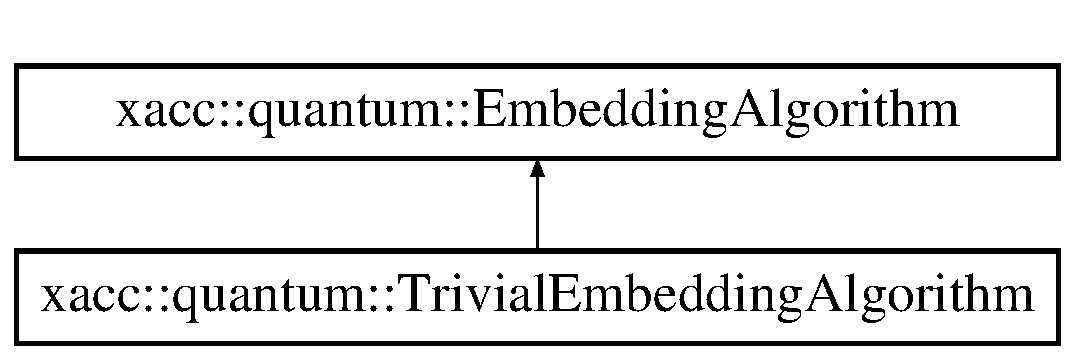
\includegraphics[height=4.000000cm]{a00083}
\end{center}
\end{figure}
\subsection*{Public Member Functions}
\begin{DoxyCompactItemize}
\item 
{\bfseries Swap} (std\+::vector$<$ int $>$ \hyperlink{a00042_a2a56be6c2519ea65df4d06f4abae1393}{qbits})\hypertarget{a00083_a5c35a23a635f235a5615be65e769c121}{}\label{a00083_a5c35a23a635f235a5615be65e769c121}

\item 
{\bfseries Swap} (int control\+Qubit, int target\+Qubit)\hypertarget{a00083_ac19efe303b798e14441a2c235b5ba7f3}{}\label{a00083_ac19efe303b798e14441a2c235b5ba7f3}

\end{DoxyCompactItemize}
\subsection*{Additional Inherited Members}


The documentation for this class was generated from the following files\+:\begin{DoxyCompactItemize}
\item 
Swap.\+hpp\item 
Swap.\+cpp\end{DoxyCompactItemize}

\hypertarget{a00084}{}\section{fire\+:\+:Eigen\+Tensor\+Provider$<$ Rank, Scalar $>$ Class Template Reference}
\label{a00084}\index{fire\+::\+Eigen\+Tensor\+Provider$<$ Rank, Scalar $>$@{fire\+::\+Eigen\+Tensor\+Provider$<$ Rank, Scalar $>$}}


{\ttfamily \#include $<$Eigen\+Tensor\+Provider.\+hpp$>$}

Inheritance diagram for fire\+:\+:Eigen\+Tensor\+Provider$<$ Rank, Scalar $>$\+:\begin{figure}[H]
\begin{center}
\leavevmode
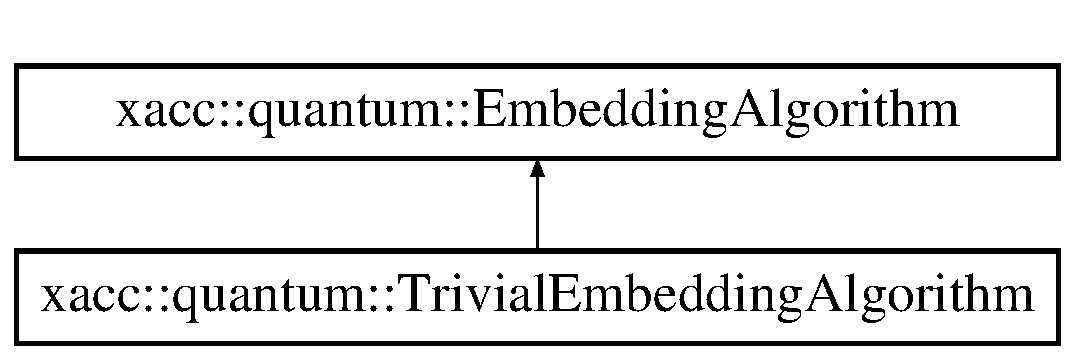
\includegraphics[height=2.000000cm]{a00084}
\end{center}
\end{figure}
\subsection*{Public Member Functions}
\begin{DoxyCompactItemize}
\item 
\hyperlink{a00084_a666937cbdec96978bdd47132a95ab9e6}{Eigen\+Tensor\+Provider} ()
\item 
{\footnotesize template$<$typename... Dimensions$>$ }\\void \hyperlink{a00084_a2d624402c063c0398f018417aae2fe28}{initialize\+Tensor\+Backend} (int first\+Dim, Dimensions...\+other\+Dims)
\item 
void \hyperlink{a00084_a284d6bb6a8539c5776e00d2a377d188e}{initialize\+Tensor\+Backend\+With\+Reference} (\hyperlink{a00822_a1bf491fd1c876e2808648b2fd291e3dd}{Tensor\+Reference}$<$ Scalar $>$ \&reference)
\item 
{\footnotesize template$<$typename... Indices$>$ }\\Scalar \& \hyperlink{a00084_abc61cda0193bc5f5d7fcf17ff8e96d82}{tensor\+Coefficient} (Indices...\+indices)
\item 
bool \hyperlink{a00084_a3e15190363627f4c6b373dc56dd2b4f3}{check\+Equality} (\hyperlink{a00822_a1bf491fd1c876e2808648b2fd291e3dd}{Tensor\+Reference}$<$ Scalar $>$ \&other)
\item 
{\footnotesize template$<$typename Other\+Derived , typename Contraction\+Dims $>$ }\\\hyperlink{a00822_a1bf491fd1c876e2808648b2fd291e3dd}{Tensor\+Reference}$<$ Scalar $>$ \hyperlink{a00084_acd9f39dacb5fd6c35f3f840ed22194e9}{execute\+Contraction} (Other\+Derived \&t2, Contraction\+Dims \&c\+Indices)
\item 
Scalar $\ast$ \hyperlink{a00084_aff5626be9e55f593f0a6b71174ecbd8a}{data} ()
\item 
\hyperlink{a00822_a1bf491fd1c876e2808648b2fd291e3dd}{Tensor\+Reference}$<$ Scalar $>$ \hyperlink{a00084_a957d54e0259b1ea798a47389af4b8379}{add} (\hyperlink{a00822_a1bf491fd1c876e2808648b2fd291e3dd}{Tensor\+Reference}$<$ Scalar $>$ \&other)
\item 
{\footnotesize template$<$typename Init\+List $>$ }\\void \hyperlink{a00084_a3d02dbf7e2d255a1378084aa6459cf25}{set\+Tensor\+Values} (Init\+List \&vals)
\item 
void \hyperlink{a00084_a607ad28d9f0b8b7f639dc1b0693dfd03}{print\+Tensor} (std\+::ostream \&stream)
\item 
void \hyperlink{a00084_a461c3348c66ae011167d8c194c79dce9}{fill\+With\+Random\+Values} ()
\item 
\hyperlink{a00822_a1bf491fd1c876e2808648b2fd291e3dd}{Tensor\+Reference}$<$ Scalar $>$ \hyperlink{a00084_ae526f2376663adc8788ba8f4c04eb6cb}{scalar\+Product} (Scalar \&val)
\item 
{\footnotesize template$<$typename Dim\+Array $>$ }\\\hyperlink{a00822_a1bf491fd1c876e2808648b2fd291e3dd}{Tensor\+Reference}$<$ Scalar $>$ \hyperlink{a00084_a5ffd64a2a2a7b5886b2175d21a46dccf}{reshape\+Tensor} (Dim\+Array \&array)
\item 
{\footnotesize template$<$typename Dim\+Array $>$ }\\\hyperlink{a00822_a1bf491fd1c876e2808648b2fd291e3dd}{Tensor\+Reference}$<$ Scalar $>$ {\bfseries shuffle\+Tensor} (Dim\+Array \&array)\hypertarget{a00084_ac4d85c2ce0bfb666ddb7284241b74dcb}{}\label{a00084_ac4d85c2ce0bfb666ddb7284241b74dcb}

\item 
std\+::tuple$<$ \hyperlink{a00822_a1bf491fd1c876e2808648b2fd291e3dd}{Tensor\+Reference}$<$ Scalar $>$, \hyperlink{a00822_a1bf491fd1c876e2808648b2fd291e3dd}{Tensor\+Reference}$<$ Scalar $>$, \hyperlink{a00822_a1bf491fd1c876e2808648b2fd291e3dd}{Tensor\+Reference}$<$ Scalar $>$ $>$ {\bfseries compute\+Svd} (\hyperlink{a00822_a1bf491fd1c876e2808648b2fd291e3dd}{Tensor\+Reference}$<$ Scalar $>$ \&ref, double cutoff)\hypertarget{a00084_aa1ba881990a0af6e0a68f8927f94c89d}{}\label{a00084_aa1ba881990a0af6e0a68f8927f94c89d}

\item 
\hyperlink{a00822_a1bf491fd1c876e2808648b2fd291e3dd}{Tensor\+Reference}$<$ Scalar $>$ {\bfseries kron\+Prod} (\hyperlink{a00822_a1bf491fd1c876e2808648b2fd291e3dd}{Tensor\+Reference}$<$ Scalar $>$ \&other)\hypertarget{a00084_ade4eea42a36aaa42cb8ea85ae3dee711}{}\label{a00084_ade4eea42a36aaa42cb8ea85ae3dee711}

\end{DoxyCompactItemize}
\subsection*{Static Public Member Functions}
\begin{DoxyCompactItemize}
\item 
static constexpr int \hyperlink{a00084_a68f0ad7ead91dec2ea56f173981465c8}{get\+Rank} ()
\end{DoxyCompactItemize}
\subsection*{Static Public Attributes}
\begin{DoxyCompactItemize}
\item 
static const int \hyperlink{a00084_ae8f0217985d78dba31d7bdb95ace1e43}{rank} = Rank
\end{DoxyCompactItemize}


\subsection{Detailed Description}
\subsubsection*{template$<$const int Rank, typename Scalar = double$>$\\*
class fire\+::\+Eigen\+Tensor\+Provider$<$ Rank, Scalar $>$}

The \hyperlink{a00084}{Eigen\+Tensor\+Provider} is a \hyperlink{a00300}{Tensor\+Provider} that provides tensor data and operations using the Eigen C++ tensor module. 

\subsection{Constructor \& Destructor Documentation}
\index{fire\+::\+Eigen\+Tensor\+Provider@{fire\+::\+Eigen\+Tensor\+Provider}!Eigen\+Tensor\+Provider@{Eigen\+Tensor\+Provider}}
\index{Eigen\+Tensor\+Provider@{Eigen\+Tensor\+Provider}!fire\+::\+Eigen\+Tensor\+Provider@{fire\+::\+Eigen\+Tensor\+Provider}}
\subsubsection[{\texorpdfstring{Eigen\+Tensor\+Provider()}{EigenTensorProvider()}}]{\setlength{\rightskip}{0pt plus 5cm}template$<$const int Rank, typename Scalar = double$>$ {\bf fire\+::\+Eigen\+Tensor\+Provider}$<$ Rank, Scalar $>$\+::{\bf Eigen\+Tensor\+Provider} (
\begin{DoxyParamCaption}
{}
\end{DoxyParamCaption}
)\hspace{0.3cm}{\ttfamily [inline]}}\hypertarget{a00084_a666937cbdec96978bdd47132a95ab9e6}{}\label{a00084_a666937cbdec96978bdd47132a95ab9e6}
The Constructor 

\subsection{Member Function Documentation}
\index{fire\+::\+Eigen\+Tensor\+Provider@{fire\+::\+Eigen\+Tensor\+Provider}!add@{add}}
\index{add@{add}!fire\+::\+Eigen\+Tensor\+Provider@{fire\+::\+Eigen\+Tensor\+Provider}}
\subsubsection[{\texorpdfstring{add(\+Tensor\+Reference$<$ Scalar $>$ \&other)}{add(TensorReference< Scalar > \&other)}}]{\setlength{\rightskip}{0pt plus 5cm}template$<$const int Rank, typename Scalar = double$>$ {\bf Tensor\+Reference}$<$Scalar$>$ {\bf fire\+::\+Eigen\+Tensor\+Provider}$<$ Rank, Scalar $>$\+::add (
\begin{DoxyParamCaption}
\item[{{\bf Tensor\+Reference}$<$ Scalar $>$ \&}]{other}
\end{DoxyParamCaption}
)\hspace{0.3cm}{\ttfamily [inline]}}\hypertarget{a00084_a957d54e0259b1ea798a47389af4b8379}{}\label{a00084_a957d54e0259b1ea798a47389af4b8379}
Return a Tensor\+Reference representing the sum of this Eigen \hyperlink{a00299}{Tensor} and an Eigen \hyperlink{a00299}{Tensor} represented by the other Tensor\+Reference.


\begin{DoxyParams}{Parameters}
{\em other} & Tensor\+Reference view of the other \hyperlink{a00299}{Tensor} \\
\hline
\end{DoxyParams}
\begin{DoxyReturn}{Returns}
result A new Tensor\+Reference representing the sum of this and other. 
\end{DoxyReturn}
\index{fire\+::\+Eigen\+Tensor\+Provider@{fire\+::\+Eigen\+Tensor\+Provider}!check\+Equality@{check\+Equality}}
\index{check\+Equality@{check\+Equality}!fire\+::\+Eigen\+Tensor\+Provider@{fire\+::\+Eigen\+Tensor\+Provider}}
\subsubsection[{\texorpdfstring{check\+Equality(\+Tensor\+Reference$<$ Scalar $>$ \&other)}{checkEquality(TensorReference< Scalar > \&other)}}]{\setlength{\rightskip}{0pt plus 5cm}template$<$const int Rank, typename Scalar = double$>$ bool {\bf fire\+::\+Eigen\+Tensor\+Provider}$<$ Rank, Scalar $>$\+::check\+Equality (
\begin{DoxyParamCaption}
\item[{{\bf Tensor\+Reference}$<$ Scalar $>$ \&}]{other}
\end{DoxyParamCaption}
)\hspace{0.3cm}{\ttfamily [inline]}}\hypertarget{a00084_a3e15190363627f4c6b373dc56dd2b4f3}{}\label{a00084_a3e15190363627f4c6b373dc56dd2b4f3}
Return true if the provided Tensor\+Reference as a tensor is equal to this tensor.


\begin{DoxyParams}{Parameters}
{\em other} & Tensor\+Reference view of the other \hyperlink{a00299}{Tensor} \\
\hline
\end{DoxyParams}
\begin{DoxyReturn}{Returns}
equal A boolean indicating if these Tensors are equal 
\end{DoxyReturn}
\index{fire\+::\+Eigen\+Tensor\+Provider@{fire\+::\+Eigen\+Tensor\+Provider}!data@{data}}
\index{data@{data}!fire\+::\+Eigen\+Tensor\+Provider@{fire\+::\+Eigen\+Tensor\+Provider}}
\subsubsection[{\texorpdfstring{data()}{data()}}]{\setlength{\rightskip}{0pt plus 5cm}template$<$const int Rank, typename Scalar = double$>$ Scalar$\ast$ {\bf fire\+::\+Eigen\+Tensor\+Provider}$<$ Rank, Scalar $>$\+::data (
\begin{DoxyParamCaption}
{}
\end{DoxyParamCaption}
)\hspace{0.3cm}{\ttfamily [inline]}}\hypertarget{a00084_aff5626be9e55f593f0a6b71174ecbd8a}{}\label{a00084_aff5626be9e55f593f0a6b71174ecbd8a}
Return the 1-\/D array wrapped by this Eigen \hyperlink{a00299}{Tensor}

\begin{DoxyReturn}{Returns}
data 1-\/D array of data representing the tensor in this \hyperlink{a00300}{Tensor\+Provider} 
\end{DoxyReturn}
\index{fire\+::\+Eigen\+Tensor\+Provider@{fire\+::\+Eigen\+Tensor\+Provider}!execute\+Contraction@{execute\+Contraction}}
\index{execute\+Contraction@{execute\+Contraction}!fire\+::\+Eigen\+Tensor\+Provider@{fire\+::\+Eigen\+Tensor\+Provider}}
\subsubsection[{\texorpdfstring{execute\+Contraction(\+Other\+Derived \&t2, Contraction\+Dims \&c\+Indices)}{executeContraction(OtherDerived \&t2, ContractionDims \&cIndices)}}]{\setlength{\rightskip}{0pt plus 5cm}template$<$const int Rank, typename Scalar = double$>$ template$<$typename Other\+Derived , typename Contraction\+Dims $>$ {\bf Tensor\+Reference}$<$Scalar$>$ {\bf fire\+::\+Eigen\+Tensor\+Provider}$<$ Rank, Scalar $>$\+::execute\+Contraction (
\begin{DoxyParamCaption}
\item[{Other\+Derived \&}]{t2, }
\item[{Contraction\+Dims \&}]{c\+Indices}
\end{DoxyParamCaption}
)\hspace{0.3cm}{\ttfamily [inline]}}\hypertarget{a00084_acd9f39dacb5fd6c35f3f840ed22194e9}{}\label{a00084_acd9f39dacb5fd6c35f3f840ed22194e9}
Compute the tensor contraction of this Eigen \hyperlink{a00299}{Tensor} with the provided Other \hyperlink{a00299}{Tensor}.


\begin{DoxyParams}{Parameters}
{\em t2} & The other \hyperlink{a00299}{Tensor} \\
\hline
{\em indices} & The contraction indices. \\
\hline
\end{DoxyParams}
\begin{DoxyReturn}{Returns}
result The contraction result as a Tensor\+Reference 
\end{DoxyReturn}
\index{fire\+::\+Eigen\+Tensor\+Provider@{fire\+::\+Eigen\+Tensor\+Provider}!fill\+With\+Random\+Values@{fill\+With\+Random\+Values}}
\index{fill\+With\+Random\+Values@{fill\+With\+Random\+Values}!fire\+::\+Eigen\+Tensor\+Provider@{fire\+::\+Eigen\+Tensor\+Provider}}
\subsubsection[{\texorpdfstring{fill\+With\+Random\+Values()}{fillWithRandomValues()}}]{\setlength{\rightskip}{0pt plus 5cm}template$<$const int Rank, typename Scalar = double$>$ void {\bf fire\+::\+Eigen\+Tensor\+Provider}$<$ Rank, Scalar $>$\+::fill\+With\+Random\+Values (
\begin{DoxyParamCaption}
{}
\end{DoxyParamCaption}
)\hspace{0.3cm}{\ttfamily [inline]}}\hypertarget{a00084_a461c3348c66ae011167d8c194c79dce9}{}\label{a00084_a461c3348c66ae011167d8c194c79dce9}
Set the Eigen \hyperlink{a00299}{Tensor} values to random values. \index{fire\+::\+Eigen\+Tensor\+Provider@{fire\+::\+Eigen\+Tensor\+Provider}!get\+Rank@{get\+Rank}}
\index{get\+Rank@{get\+Rank}!fire\+::\+Eigen\+Tensor\+Provider@{fire\+::\+Eigen\+Tensor\+Provider}}
\subsubsection[{\texorpdfstring{get\+Rank()}{getRank()}}]{\setlength{\rightskip}{0pt plus 5cm}template$<$const int Rank, typename Scalar = double$>$ static constexpr int {\bf fire\+::\+Eigen\+Tensor\+Provider}$<$ Rank, Scalar $>$\+::get\+Rank (
\begin{DoxyParamCaption}
{}
\end{DoxyParamCaption}
)\hspace{0.3cm}{\ttfamily [inline]}, {\ttfamily [static]}}\hypertarget{a00084_a68f0ad7ead91dec2ea56f173981465c8}{}\label{a00084_a68f0ad7ead91dec2ea56f173981465c8}
Return the rank of this Eigen \hyperlink{a00299}{Tensor}

\begin{DoxyReturn}{Returns}
rank The rank of this \hyperlink{a00299}{Tensor} 
\end{DoxyReturn}
\index{fire\+::\+Eigen\+Tensor\+Provider@{fire\+::\+Eigen\+Tensor\+Provider}!initialize\+Tensor\+Backend@{initialize\+Tensor\+Backend}}
\index{initialize\+Tensor\+Backend@{initialize\+Tensor\+Backend}!fire\+::\+Eigen\+Tensor\+Provider@{fire\+::\+Eigen\+Tensor\+Provider}}
\subsubsection[{\texorpdfstring{initialize\+Tensor\+Backend(int first\+Dim, Dimensions...\+other\+Dims)}{initializeTensorBackend(int firstDim, Dimensions...otherDims)}}]{\setlength{\rightskip}{0pt plus 5cm}template$<$const int Rank, typename Scalar = double$>$ template$<$typename... Dimensions$>$ void {\bf fire\+::\+Eigen\+Tensor\+Provider}$<$ Rank, Scalar $>$\+::initialize\+Tensor\+Backend (
\begin{DoxyParamCaption}
\item[{int}]{first\+Dim, }
\item[{Dimensions...}]{other\+Dims}
\end{DoxyParamCaption}
)\hspace{0.3cm}{\ttfamily [inline]}}\hypertarget{a00084_a2d624402c063c0398f018417aae2fe28}{}\label{a00084_a2d624402c063c0398f018417aae2fe28}
Initialize the Eigen \hyperlink{a00299}{Tensor} with all zeros. 
\begin{DoxyParams}{Parameters}
{\em first\+Dim} & \\
\hline
{\em other\+Dims} & \\
\hline
\end{DoxyParams}
\index{fire\+::\+Eigen\+Tensor\+Provider@{fire\+::\+Eigen\+Tensor\+Provider}!initialize\+Tensor\+Backend\+With\+Reference@{initialize\+Tensor\+Backend\+With\+Reference}}
\index{initialize\+Tensor\+Backend\+With\+Reference@{initialize\+Tensor\+Backend\+With\+Reference}!fire\+::\+Eigen\+Tensor\+Provider@{fire\+::\+Eigen\+Tensor\+Provider}}
\subsubsection[{\texorpdfstring{initialize\+Tensor\+Backend\+With\+Reference(\+Tensor\+Reference$<$ Scalar $>$ \&reference)}{initializeTensorBackendWithReference(TensorReference< Scalar > \&reference)}}]{\setlength{\rightskip}{0pt plus 5cm}template$<$const int Rank, typename Scalar = double$>$ void {\bf fire\+::\+Eigen\+Tensor\+Provider}$<$ Rank, Scalar $>$\+::initialize\+Tensor\+Backend\+With\+Reference (
\begin{DoxyParamCaption}
\item[{{\bf Tensor\+Reference}$<$ Scalar $>$ \&}]{reference}
\end{DoxyParamCaption}
)\hspace{0.3cm}{\ttfamily [inline]}}\hypertarget{a00084_a284d6bb6a8539c5776e00d2a377d188e}{}\label{a00084_a284d6bb6a8539c5776e00d2a377d188e}
Initialize the Eigen \hyperlink{a00299}{Tensor} from an existing Tensor\+Reference 
\begin{DoxyParams}{Parameters}
{\em reference} & \\
\hline
\end{DoxyParams}
\index{fire\+::\+Eigen\+Tensor\+Provider@{fire\+::\+Eigen\+Tensor\+Provider}!print\+Tensor@{print\+Tensor}}
\index{print\+Tensor@{print\+Tensor}!fire\+::\+Eigen\+Tensor\+Provider@{fire\+::\+Eigen\+Tensor\+Provider}}
\subsubsection[{\texorpdfstring{print\+Tensor(std\+::ostream \&stream)}{printTensor(std::ostream \&stream)}}]{\setlength{\rightskip}{0pt plus 5cm}template$<$const int Rank, typename Scalar = double$>$ void {\bf fire\+::\+Eigen\+Tensor\+Provider}$<$ Rank, Scalar $>$\+::print\+Tensor (
\begin{DoxyParamCaption}
\item[{std\+::ostream \&}]{stream}
\end{DoxyParamCaption}
)\hspace{0.3cm}{\ttfamily [inline]}}\hypertarget{a00084_a607ad28d9f0b8b7f639dc1b0693dfd03}{}\label{a00084_a607ad28d9f0b8b7f639dc1b0693dfd03}
Output this Eigen \hyperlink{a00299}{Tensor} to the provided output stream.


\begin{DoxyParams}{Parameters}
{\em output\+Stream} & The output stream to write the tensor to. \\
\hline
\end{DoxyParams}
\index{fire\+::\+Eigen\+Tensor\+Provider@{fire\+::\+Eigen\+Tensor\+Provider}!reshape\+Tensor@{reshape\+Tensor}}
\index{reshape\+Tensor@{reshape\+Tensor}!fire\+::\+Eigen\+Tensor\+Provider@{fire\+::\+Eigen\+Tensor\+Provider}}
\subsubsection[{\texorpdfstring{reshape\+Tensor(\+Dim\+Array \&array)}{reshapeTensor(DimArray \&array)}}]{\setlength{\rightskip}{0pt plus 5cm}template$<$const int Rank, typename Scalar = double$>$ template$<$typename Dim\+Array $>$ {\bf Tensor\+Reference}$<$Scalar$>$ {\bf fire\+::\+Eigen\+Tensor\+Provider}$<$ Rank, Scalar $>$\+::reshape\+Tensor (
\begin{DoxyParamCaption}
\item[{Dim\+Array \&}]{array}
\end{DoxyParamCaption}
)\hspace{0.3cm}{\ttfamily [inline]}}\hypertarget{a00084_a5ffd64a2a2a7b5886b2175d21a46dccf}{}\label{a00084_a5ffd64a2a2a7b5886b2175d21a46dccf}
Reshape the Eigen \hyperlink{a00299}{Tensor} with a new array of dimensions


\begin{DoxyParams}{Parameters}
{\em array} & Array of new dimensions for each rank index \\
\hline
\end{DoxyParams}
\begin{DoxyReturn}{Returns}
reshaped\+Tensor A Tensor\+Reference representing new reshaped tensor. 
\end{DoxyReturn}
\index{fire\+::\+Eigen\+Tensor\+Provider@{fire\+::\+Eigen\+Tensor\+Provider}!scalar\+Product@{scalar\+Product}}
\index{scalar\+Product@{scalar\+Product}!fire\+::\+Eigen\+Tensor\+Provider@{fire\+::\+Eigen\+Tensor\+Provider}}
\subsubsection[{\texorpdfstring{scalar\+Product(\+Scalar \&val)}{scalarProduct(Scalar \&val)}}]{\setlength{\rightskip}{0pt plus 5cm}template$<$const int Rank, typename Scalar = double$>$ {\bf Tensor\+Reference}$<$Scalar$>$ {\bf fire\+::\+Eigen\+Tensor\+Provider}$<$ Rank, Scalar $>$\+::scalar\+Product (
\begin{DoxyParamCaption}
\item[{Scalar \&}]{val}
\end{DoxyParamCaption}
)\hspace{0.3cm}{\ttfamily [inline]}}\hypertarget{a00084_ae526f2376663adc8788ba8f4c04eb6cb}{}\label{a00084_ae526f2376663adc8788ba8f4c04eb6cb}
Multiply all elements of this Eigen \hyperlink{a00299}{Tensor} by the provided Scalar.


\begin{DoxyParams}{Parameters}
{\em val} & Scalar to multiply this tensor by. \\
\hline
\end{DoxyParams}
\begin{DoxyReturn}{Returns}
result A Tensor\+Reference representing the result 
\end{DoxyReturn}
\index{fire\+::\+Eigen\+Tensor\+Provider@{fire\+::\+Eigen\+Tensor\+Provider}!set\+Tensor\+Values@{set\+Tensor\+Values}}
\index{set\+Tensor\+Values@{set\+Tensor\+Values}!fire\+::\+Eigen\+Tensor\+Provider@{fire\+::\+Eigen\+Tensor\+Provider}}
\subsubsection[{\texorpdfstring{set\+Tensor\+Values(\+Init\+List \&vals)}{setTensorValues(InitList \&vals)}}]{\setlength{\rightskip}{0pt plus 5cm}template$<$const int Rank, typename Scalar = double$>$ template$<$typename Init\+List $>$ void {\bf fire\+::\+Eigen\+Tensor\+Provider}$<$ Rank, Scalar $>$\+::set\+Tensor\+Values (
\begin{DoxyParamCaption}
\item[{Init\+List \&}]{vals}
\end{DoxyParamCaption}
)\hspace{0.3cm}{\ttfamily [inline]}}\hypertarget{a00084_a3d02dbf7e2d255a1378084aa6459cf25}{}\label{a00084_a3d02dbf7e2d255a1378084aa6459cf25}
Set the Eigen \hyperlink{a00299}{Tensor} values using nested initializer\+\_\+list


\begin{DoxyParams}{Parameters}
{\em vals} & The values as a nest std\+::initializer\+\_\+lists \\
\hline
\end{DoxyParams}
\index{fire\+::\+Eigen\+Tensor\+Provider@{fire\+::\+Eigen\+Tensor\+Provider}!tensor\+Coefficient@{tensor\+Coefficient}}
\index{tensor\+Coefficient@{tensor\+Coefficient}!fire\+::\+Eigen\+Tensor\+Provider@{fire\+::\+Eigen\+Tensor\+Provider}}
\subsubsection[{\texorpdfstring{tensor\+Coefficient(\+Indices...\+indices)}{tensorCoefficient(Indices...indices)}}]{\setlength{\rightskip}{0pt plus 5cm}template$<$const int Rank, typename Scalar = double$>$ template$<$typename... Indices$>$ Scalar\& {\bf fire\+::\+Eigen\+Tensor\+Provider}$<$ Rank, Scalar $>$\+::tensor\+Coefficient (
\begin{DoxyParamCaption}
\item[{Indices...}]{indices}
\end{DoxyParamCaption}
)\hspace{0.3cm}{\ttfamily [inline]}}\hypertarget{a00084_abc61cda0193bc5f5d7fcf17ff8e96d82}{}\label{a00084_abc61cda0193bc5f5d7fcf17ff8e96d82}
Return the coefficient at the given tensor indices.


\begin{DoxyParams}{Parameters}
{\em indices} & The indices for the desired value \\
\hline
\end{DoxyParams}
\begin{DoxyReturn}{Returns}
val The value at the indices. 
\end{DoxyReturn}


\subsection{Member Data Documentation}
\index{fire\+::\+Eigen\+Tensor\+Provider@{fire\+::\+Eigen\+Tensor\+Provider}!rank@{rank}}
\index{rank@{rank}!fire\+::\+Eigen\+Tensor\+Provider@{fire\+::\+Eigen\+Tensor\+Provider}}
\subsubsection[{\texorpdfstring{rank}{rank}}]{\setlength{\rightskip}{0pt plus 5cm}template$<$const int Rank, typename Scalar = double$>$ const int {\bf fire\+::\+Eigen\+Tensor\+Provider}$<$ Rank, Scalar $>$\+::rank = Rank\hspace{0.3cm}{\ttfamily [static]}}\hypertarget{a00084_ae8f0217985d78dba31d7bdb95ace1e43}{}\label{a00084_ae8f0217985d78dba31d7bdb95ace1e43}
Static reference to the rank of the tensor wrapped by this provider 

The documentation for this class was generated from the following file\+:\begin{DoxyCompactItemize}
\item 
Eigen\+Tensor\+Provider.\+hpp\end{DoxyCompactItemize}

\hypertarget{a00085}{}\section{xacc\+:\+:X\+A\+C\+C\+Vertex$<$ Properties $>$ Class Template Reference}
\label{a00085}\index{xacc\+::\+X\+A\+C\+C\+Vertex$<$ Properties $>$@{xacc\+::\+X\+A\+C\+C\+Vertex$<$ Properties $>$}}


{\ttfamily \#include $<$Graph.\+hpp$>$}

\subsection*{Public Member Functions}
\begin{DoxyCompactItemize}
\item 
std\+::string {\bfseries get\+Property\+Name} (const int index)\hypertarget{a00085_a7a7c4d60a277c3c0998f3911d128eaa5}{}\label{a00085_a7a7c4d60a277c3c0998f3911d128eaa5}

\end{DoxyCompactItemize}
\subsection*{Public Attributes}
\begin{DoxyCompactItemize}
\item 
std\+::tuple$<$ Properties... $>$ {\bfseries properties}\hypertarget{a00085_ad97a32f3cfcceef3eb0725a1a185025b}{}\label{a00085_ad97a32f3cfcceef3eb0725a1a185025b}

\item 
std\+::vector$<$ std\+::string $>$ {\bfseries property\+Names}\hypertarget{a00085_a9107342e37aaa5d7936d7e457051f461}{}\label{a00085_a9107342e37aaa5d7936d7e457051f461}

\end{DoxyCompactItemize}


\subsection{Detailed Description}
\subsubsection*{template$<$typename... Properties$>$\\*
class xacc\+::\+X\+A\+C\+C\+Vertex$<$ Properties $>$}

The base class of all Q\+CI Vertices for the Q\+CI Common \hyperlink{a00043}{Graph} class. All Vertices must keep track of a set of properties, stored as a tuple. 

The documentation for this class was generated from the following file\+:\begin{DoxyCompactItemize}
\item 
Graph.\+hpp\end{DoxyCompactItemize}

\hypertarget{a00086}{}\section{xacc\+:\+:Graph$<$ Vertex, type $>$\+:\+:X\+A\+C\+C\+Vertex\+Properties\+Writer Class Reference}
\label{a00086}\index{xacc\+::\+Graph$<$ Vertex, type $>$\+::\+X\+A\+C\+C\+Vertex\+Properties\+Writer@{xacc\+::\+Graph$<$ Vertex, type $>$\+::\+X\+A\+C\+C\+Vertex\+Properties\+Writer}}


{\ttfamily \#include $<$Graph.\+hpp$>$}

\subsection*{Public Member Functions}
\begin{DoxyCompactItemize}
\item 
{\bfseries X\+A\+C\+C\+Vertex\+Properties\+Writer} (adj\+\_\+list \&list)\hypertarget{a00086_a5f8d68a2293a5b545d5a3eb0220e25ef}{}\label{a00086_a5f8d68a2293a5b545d5a3eb0220e25ef}

\item 
{\footnotesize template$<$class Boost\+Vertex $>$ }\\void {\bfseries operator()} (std\+::ostream \&out, const Boost\+Vertex \&v) const \hypertarget{a00086_abafd279805601c438fe608f620b149a3}{}\label{a00086_abafd279805601c438fe608f620b149a3}

\end{DoxyCompactItemize}
\subsection*{Protected Attributes}
\begin{DoxyCompactItemize}
\item 
adj\+\_\+list {\bfseries graph}\hypertarget{a00086_ac74a285698deb2e93f028474c5c92085}{}\label{a00086_ac74a285698deb2e93f028474c5c92085}

\end{DoxyCompactItemize}


\subsection{Detailed Description}
\subsubsection*{template$<$typename Vertex, Graph\+Type type = Undirected$>$\\*
class xacc\+::\+Graph$<$ Vertex, type $>$\+::\+X\+A\+C\+C\+Vertex\+Properties\+Writer}

This is a custom utility class for writing X\+A\+C\+C\+Vertices with user-\/defined properties. 

The documentation for this class was generated from the following file\+:\begin{DoxyCompactItemize}
\item 
Graph.\+hpp\end{DoxyCompactItemize}

\hypertarget{a00087}{}\section{boost\+:\+:dll\+:\+:detail\+:\+:Elf\+\_\+\+Shdr\+\_\+template$<$ Address\+OffsetT $>$ Struct Template Reference}
\label{a00087}\index{boost\+::dll\+::detail\+::\+Elf\+\_\+\+Shdr\+\_\+template$<$ Address\+Offset\+T $>$@{boost\+::dll\+::detail\+::\+Elf\+\_\+\+Shdr\+\_\+template$<$ Address\+Offset\+T $>$}}
\subsection*{Public Attributes}
\begin{DoxyCompactItemize}
\item 
boost\+::uint32\+\_\+t {\bfseries sh\+\_\+name}\hypertarget{a00087_af74b85fd375874942acab42fb236938b}{}\label{a00087_af74b85fd375874942acab42fb236938b}

\item 
boost\+::uint32\+\_\+t {\bfseries sh\+\_\+type}\hypertarget{a00087_aef81ee9415e932f037457039ecb6062a}{}\label{a00087_aef81ee9415e932f037457039ecb6062a}

\item 
Address\+OffsetT {\bfseries sh\+\_\+flags}\hypertarget{a00087_a0cf665258d1353d703dbe5f03b06377c}{}\label{a00087_a0cf665258d1353d703dbe5f03b06377c}

\item 
Address\+OffsetT {\bfseries sh\+\_\+addr}\hypertarget{a00087_a96484407d371204d2cdf512c946a3035}{}\label{a00087_a96484407d371204d2cdf512c946a3035}

\item 
Address\+OffsetT {\bfseries sh\+\_\+offset}\hypertarget{a00087_a218d431d671c785239cbe32d5f566329}{}\label{a00087_a218d431d671c785239cbe32d5f566329}

\item 
Address\+OffsetT {\bfseries sh\+\_\+size}\hypertarget{a00087_a0e8fbbadfb65a2c456951a632a114b0f}{}\label{a00087_a0e8fbbadfb65a2c456951a632a114b0f}

\item 
boost\+::uint32\+\_\+t {\bfseries sh\+\_\+link}\hypertarget{a00087_a0f3c4d6a3f6db4ce3debe84bfab65aa4}{}\label{a00087_a0f3c4d6a3f6db4ce3debe84bfab65aa4}

\item 
boost\+::uint32\+\_\+t {\bfseries sh\+\_\+info}\hypertarget{a00087_ab2ae82258ef53873e52f5711efd46f69}{}\label{a00087_ab2ae82258ef53873e52f5711efd46f69}

\item 
Address\+OffsetT {\bfseries sh\+\_\+addralign}\hypertarget{a00087_a8b78c53bdbdd717f69a20f53427d99d5}{}\label{a00087_a8b78c53bdbdd717f69a20f53427d99d5}

\item 
Address\+OffsetT {\bfseries sh\+\_\+entsize}\hypertarget{a00087_a736b1d41e2034475f8dcf3119614e88d}{}\label{a00087_a736b1d41e2034475f8dcf3119614e88d}

\end{DoxyCompactItemize}


The documentation for this struct was generated from the following file\+:\begin{DoxyCompactItemize}
\item 
elf\+\_\+info.\+hpp\end{DoxyCompactItemize}

\hypertarget{a00088}{}\section{M\+S\+C\+Embedding Class Reference}
\label{a00088}\index{M\+S\+C\+Embedding@{M\+S\+C\+Embedding}}
Inheritance diagram for M\+S\+C\+Embedding\+:\begin{figure}[H]
\begin{center}
\leavevmode
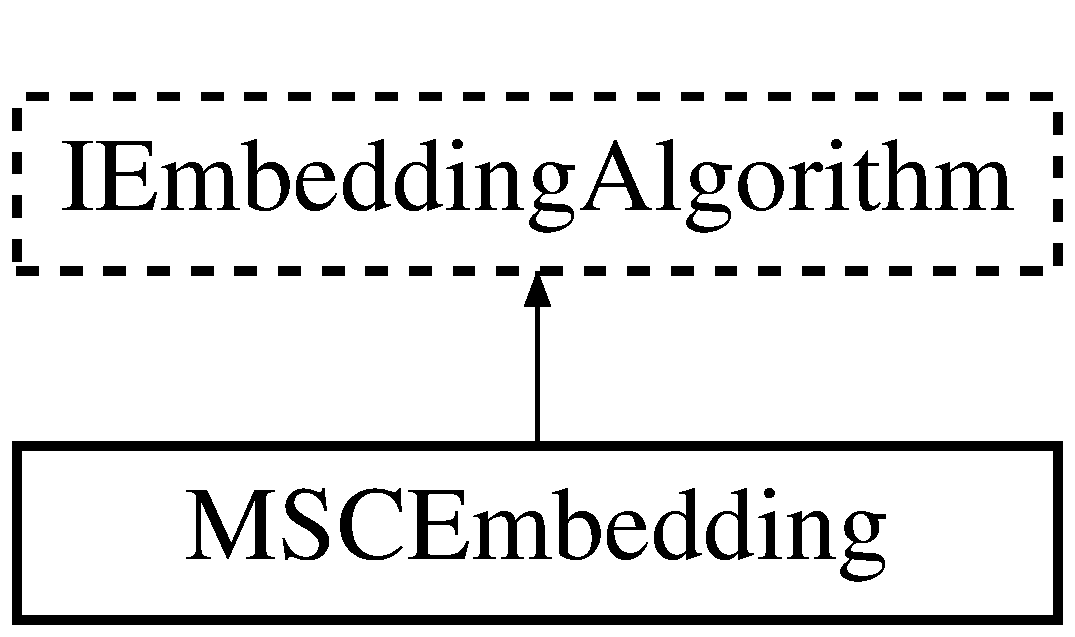
\includegraphics[height=2.000000cm]{a00088}
\end{center}
\end{figure}
\subsection*{Public Member Functions}
\begin{DoxyCompactItemize}
\item 
\hyperlink{a00088_a121cd4bb6ed8a7f520070482a2954c46}{M\+S\+C\+Embedding} (\hyperlink{a00076}{I\+Quell\+E\+Graph} \&prob, \hyperlink{a00076}{I\+Quell\+E\+Graph} \&\hyperlink{a00071_aacf081e6ad5824b339b212844eb61b63}{hardware})
\item 
virtual std\+::shared\+\_\+ptr$<$ \hyperlink{a00050}{Embedding} $>$ \hyperlink{a00088_ad1d4dd78521d916ce370ab4b109c5222}{compute\+Embedding} (std\+::map$<$ std\+::string, std\+::string $>$ parameters=std\+::map$<$ std\+::string, std\+::string $>$())
\item 
virtual std\+::string \hyperlink{a00088_a584852f9b912480086b27c1f1f14274e}{get\+Algorithm\+Name} ()
\end{DoxyCompactItemize}
\subsection*{Additional Inherited Members}


\subsection{Constructor \& Destructor Documentation}
\index{M\+S\+C\+Embedding@{M\+S\+C\+Embedding}!M\+S\+C\+Embedding@{M\+S\+C\+Embedding}}
\index{M\+S\+C\+Embedding@{M\+S\+C\+Embedding}!M\+S\+C\+Embedding@{M\+S\+C\+Embedding}}
\subsubsection[{\texorpdfstring{M\+S\+C\+Embedding(\+I\+Quell\+E\+Graph \&prob, I\+Quell\+E\+Graph \&hardware)}{MSCEmbedding(IQuellEGraph \&prob, IQuellEGraph \&hardware)}}]{\setlength{\rightskip}{0pt plus 5cm}M\+S\+C\+Embedding\+::\+M\+S\+C\+Embedding (
\begin{DoxyParamCaption}
\item[{{\bf I\+Quell\+E\+Graph} \&}]{prob, }
\item[{{\bf I\+Quell\+E\+Graph} \&}]{hardware}
\end{DoxyParamCaption}
)}\hypertarget{a00088_a121cd4bb6ed8a7f520070482a2954c46}{}\label{a00088_a121cd4bb6ed8a7f520070482a2954c46}
The Constructor, takes the problem and hardware used in this minor graph embedding.


\begin{DoxyParams}{Parameters}
{\em prob} & \\
\hline
{\em hardware} & \\
\hline
\end{DoxyParams}


\subsection{Member Function Documentation}
\index{M\+S\+C\+Embedding@{M\+S\+C\+Embedding}!compute\+Embedding@{compute\+Embedding}}
\index{compute\+Embedding@{compute\+Embedding}!M\+S\+C\+Embedding@{M\+S\+C\+Embedding}}
\subsubsection[{\texorpdfstring{compute\+Embedding(std\+::map$<$ std\+::string, std\+::string $>$ parameters=std\+::map$<$ std\+::string, std\+::string $>$())}{computeEmbedding(std::map< std::string, std::string > parameters=std::map< std::string, std::string >())}}]{\setlength{\rightskip}{0pt plus 5cm}std\+::shared\+\_\+ptr$<$ {\bf Embedding} $>$ M\+S\+C\+Embedding\+::compute\+Embedding (
\begin{DoxyParamCaption}
\item[{std\+::map$<$ std\+::string, std\+::string $>$}]{parameters = {\ttfamily std\+:\+:map$<$~std\+:\+:string,~std\+:\+:string$>$()}}
\end{DoxyParamCaption}
)\hspace{0.3cm}{\ttfamily [virtual]}}\hypertarget{a00088_ad1d4dd78521d916ce370ab4b109c5222}{}\label{a00088_ad1d4dd78521d916ce370ab4b109c5222}
Compute this embedding.


\begin{DoxyParams}{Parameters}
{\em parameters} & \\
\hline
\end{DoxyParams}


Implements \hyperlink{a00071_a0a56d5731381551efcb4c088bca6c817}{I\+Embedding\+Algorithm}.

\index{M\+S\+C\+Embedding@{M\+S\+C\+Embedding}!get\+Algorithm\+Name@{get\+Algorithm\+Name}}
\index{get\+Algorithm\+Name@{get\+Algorithm\+Name}!M\+S\+C\+Embedding@{M\+S\+C\+Embedding}}
\subsubsection[{\texorpdfstring{get\+Algorithm\+Name()}{getAlgorithmName()}}]{\setlength{\rightskip}{0pt plus 5cm}virtual std\+::string M\+S\+C\+Embedding\+::get\+Algorithm\+Name (
\begin{DoxyParamCaption}
{}
\end{DoxyParamCaption}
)\hspace{0.3cm}{\ttfamily [inline]}, {\ttfamily [virtual]}}\hypertarget{a00088_a584852f9b912480086b27c1f1f14274e}{}\label{a00088_a584852f9b912480086b27c1f1f14274e}
Return the name of this \hyperlink{a00050}{Embedding} Algorithm.

\begin{DoxyReturn}{Returns}

\end{DoxyReturn}


Implements \hyperlink{a00071_aac9fc812fb7e84b8a379ab5f60167f2c}{I\+Embedding\+Algorithm}.



The documentation for this class was generated from the following files\+:\begin{DoxyCompactItemize}
\item 
M\+S\+C\+Embedding.\+hpp\item 
M\+S\+C\+Embedding.\+cpp\end{DoxyCompactItemize}

\hypertarget{a00089}{}\section{xacc\+:\+:quantum\+:\+:Z Class Reference}
\label{a00089}\index{xacc\+::quantum\+::Z@{xacc\+::quantum\+::Z}}
Inheritance diagram for xacc\+:\+:quantum\+:\+:Z\+:\begin{figure}[H]
\begin{center}
\leavevmode
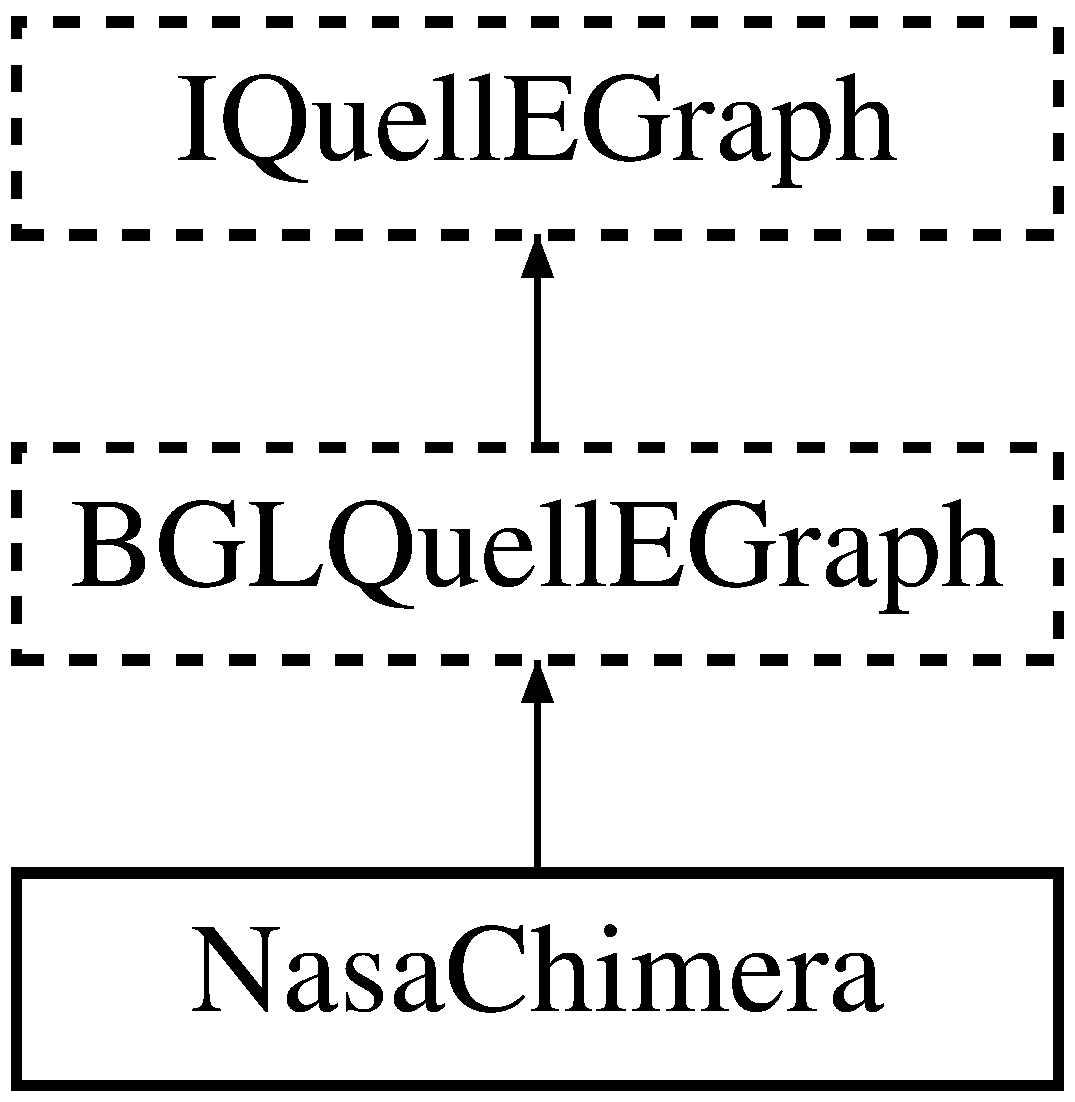
\includegraphics[height=4.000000cm]{a00089}
\end{center}
\end{figure}
\subsection*{Public Member Functions}
\begin{DoxyCompactItemize}
\item 
{\bfseries Z} (std\+::vector$<$ int $>$ qbit)\hypertarget{a00089_a5f1d311b357faed8c2665fe20cf24aeb}{}\label{a00089_a5f1d311b357faed8c2665fe20cf24aeb}

\item 
{\bfseries Z} (int qbit)\hypertarget{a00089_aa1bb7e533e7595e9ecd06879a2f8d2de}{}\label{a00089_aa1bb7e533e7595e9ecd06879a2f8d2de}

\end{DoxyCompactItemize}
\subsection*{Additional Inherited Members}


The documentation for this class was generated from the following files\+:\begin{DoxyCompactItemize}
\item 
Z.\+hpp\item 
Z.\+cpp\end{DoxyCompactItemize}

%--- End generated contents ---

% Index
\backmatter
\newpage
\phantomsection
\clearemptydoublepage
\addcontentsline{toc}{chapter}{Index}
\printindex

\end{document}
